\documentclass[12pt]{report}
\renewcommand{\baselinestretch}{1.1} 


% Define margins
\setlength{\topmargin}{-1.0cm}
\setlength{\oddsidemargin}{0.2cm}
\setlength{\textwidth}{16cm}
\setlength{\textheight}{23.0cm}






% Numbering
\makeatletter

\newcommand\frontmatter{%
	\cleardoublepage
	%\@mainmatterfalse
	\pagenumbering{roman}}

\newcommand\mainmatter{%
	\cleardoublepage
	% \@mainmattertrue
	\pagenumbering{arabic}}

\newcommand\backmatter{%
	\if@openright
	\cleardoublepage
	\else
	\clearpage
	\fi
	% \@mainmatterfalse
}

\makeatother


% Define header and footer
%\usepackage{lastpage}
%\usepackage{fancyhdr}
%\pagestyle{fancy}
%\fancyhf{}
%\lhead{{
\includegraphics[height=.8cm]{figures/nus.png}}}
%%\rhead{\textbf{\textit{Interpretable and Fair Machine Learning}} }
%\rfoot{\thepage}
%\renewcommand{\footrulewidth}{0.7pt}
%\renewcommand{\headrulewidth}{0.7pt}

% Abstract
\renewcommand\abstractname{\textsc{Abstract}}



% Packages
\usepackage{enumerate}
\usepackage{amsmath}
\usepackage{amsthm,amssymb}
\usepackage{dsfont}
\newtheorem{comment}{Comment}
\usepackage[utf8]{inputenc} 
\usepackage{graphicx}
\usepackage{multirow}
\usepackage{color}
\usepackage{comment}
\usepackage{microtype}
\usepackage{wrapfig}
\usepackage{hyperref}
\usepackage{url}
\usepackage{subfig}
\usepackage{booktabs}
\usepackage{caption}
\usepackage{enumitem,kantlipsum}
\usepackage{algorithm}
\usepackage[noend]{algpseudocode}
\usepackage{blkarray}
\usepackage{adjustbox}
\usepackage{rotating}

%Hyperlink
\hypersetup{%
	colorlinks=true,% hyperlinks will be coloured
	linkcolor=blue,% hyperlink text will be green
%	linkbordercolor=red,% hyperlink border will be red
}


% Todo packages
\usepackage{xargs}
\usepackage[pdftex,dvipsnames]{xcolor}
\usepackage[colorinlistoftodos,prependcaption,textsize=tiny]{todonotes}
\newcommandx{\unsure}[2][1=]{\todo[linecolor=red,backgroundcolor=red!25,bordercolor=red,#1]{#2}}
\newcommandx{\change}[2][1=]{\todo[linecolor=blue,backgroundcolor=blue!25,bordercolor=blue,#1]{#2}}
\newcommandx{\info}[2][1=]{\todo[linecolor=OliveGreen,backgroundcolor=OliveGreen!25,bordercolor=OliveGreen,#1]{#2}}
\newcommandx{\improvement}[2][1=]{\todo[linecolor=Plum,backgroundcolor=Plum!25,bordercolor=Plum,#1]{#2}}
\newcommandx{\thiswillnotshow}[2][1=]{\todo[disable,#1]{#2}}



% Theorem
\newtheorem{theorem}{Theorem}
\newtheorem{definition}{Definition}
\newtheorem{axiom}{Axiom}
\newtheorem{property}[theorem]{Property}
\newtheorem*{remark}{Remark}
\newtheorem{lemma}[theorem]{Lemma}
\newtheorem{lemmarep}{Lemma}
\newtheorem{proposition}[theorem]{Proposition}
\newtheorem{example}{Example}[section]
\newtheorem{corollary}{Corollary}
\newtheorem{construction}[theorem]{Construction}
\usepackage{pgfplots}


% Tikz
\usepackage{tikz}
\usetikzlibrary{automata}
\usetikzlibrary{bayesnet,arrows}
\usetikzlibrary{shapes,fit,calc,positioning}
\tikzset{box/.style={draw, diamond, thick, text centered, minimum height=0.5cm, minimum width=1cm, text width=0.9cm}}
\tikzset{line/.style={draw, thick, -latex'}}


% References
\usepackage{cite}
\usepackage[nameinlink,capitalize]{cleveref}  % easy referencing




% Macros
\newcommand{\red}[1]{\textcolor{red}{#1}}
\newcommand{\blue}[1]{\textcolor{blue}{#1}}
\newcommand{\green}[1]{\textcolor{green}{#1}}


% Fairness 
%	Justicia
			\newcommand{\justicia}{\ensuremath{\mathsf{Justicia}}}
			\newcommand{\nonsensitive}{\ensuremath{\mathbf{X}}}
			\newcommand{\sensitive}{\ensuremath{\mathbf{A}}}
			\newcommand{\bool}{\ensuremath{B}}
			\newcommand{\boolset}{\ensuremath{\mathbf{B}}}
			\newcommand{\alg}{\mathcal{M}}
			\newcommand{\R}{\ensuremath{\raisebox{\depth}{\rotatebox{180}{R}}}}
			\newcommand{\justiciaenum}{\ensuremath{\mathsf{Justicia\_enum}}}
			\newcommand{\justicialearn}{\ensuremath{\mathsf{Justicia\_infer}}}
			\newcommand{\justiciacond}{\ensuremath{\mathsf{Justicia\_cond}}}
			\newcommand{\numnonsensitive}{\ensuremath{k}}
			\newcommand{\numsensitive}{\ensuremath{m}}
			\newcommand{\abs}[1]{\ensuremath{\mid #1 \mid}}
			
	
%	FVGM
			\newcommand{\fvgm}{\ensuremath{\mathsf{FVGM}}}
			\newcommand{\mediator}{\ensuremath{\mathbf{Z}}}
			\newcommand{\stochastic}{\ensuremath{\mathsf{S3P}}}
			\DeclareMathOperator*{\argmax}{arg\,max}
			\DeclareMathOperator*{\argmin}{arg\,min}
			\newcommand{\graph}{\ensuremath{G}}
			\newcommand{\factors}{\ensuremath{\theta}}
			\newcommand{\parent}{\ensuremath{\mathrm{Pa}}}
			\newcommand{\BN}{\ensuremath{\mathsf{BN}}}
			
%	FairXplainer
			\newcommand{\fairXplainer}{\ensuremath{\mathsf{FairXplainer}}}
			\newcommand{\function}{\ensuremath{g}}
			
			
%			color
			\definecolor{terminate}{gray}{0.8}
			\definecolor{collision}{rgb}{0.2,1,0.3}
			\definecolor{existential}{rgb}{0.9,0.9, 0.1}
			\definecolor{affirmative}{rgb}{0.2,1,0.3}
			

% Interpretability
%		Relaxed CNF
			\newcommand{\Rule}{\ensuremath{{\mathcal{R}}}}
			\newcommand{\clauseweight}[1]{\ensuremath{W \! \left( #1 \right)}}
%			\newcommand{\X}{{\mathbf{X}}}
			\newcommand{\MaxSAT}{\ensuremath{\textsc{MaxSAT}}}
			\newcommand{\noise}{\xi}
			\newcommand{\card}{\eta}
			\newcommand{\noclause}{k}
			\newcommand{\crr}{\ensuremath{\mathsf{CRR}}}
			\newcommand{\CNF}{\ensuremath{\mathsf{Card2CNF}}}
%			\newcommand{\B}{\mathbf{b}}
			\newcommand{\clause}{\ensuremath{\mathsf{clause}}}
			\newcommand{\MLIC}{\ensuremath{\mathsf{MLIC}}}
			\newcommand{\IMLI}{\ensuremath{\mathsf{IMLI}}}
			\newcommand{\ILP}{\ensuremath{\textsc{ILP}}}
			
			
%		Logic
			\newcommand{\propformula}{\phi}
			\newcommand{\propclause}{C}
			\newcommand{\literal}{V}
			\newcommand{\varquantifier}{Q}
			\newcommand{\varweight}{W}
			\newcommand{\ssatformula}{\Phi}
			
%		Bayesian Network
			\newcommand{\graphvertices}{\mathbf{V}}
			\newcommand{\graphvertex}{V}
			\newcommand{\graphedges}{\mathbf{E}}
			\newcommand{\graphedge}{E}
			\newcommand{\bncomplexity}{C}
			\newcommand{\bnnumdiscrete}{\mathsf{Card}}
			
%		Dataset
			\newcommand{\dataset}{\mathbf{D}}
			\newcommand{\datadistribution}{\mathcal{D}}
			
			
			
			
			
			
			
%	    IMLI
			\newcommand{\imli}{\ensuremath{\mathsf{IMLI}}}
			
		

			
			
			
			
\title{Interpretability and Fairness in Machine Learning: A Formal Methods Approach}
\author{Bishwamittra Ghosh}
\date{}		
			


\begin{document}
	\begin{titlepage}
	\begin{center}
	\large
	Response Letter
\end{center}
We thank the reviewers for their useful comments and feedback on improving the manuscript and the presentation. In the following, we summarize changes reflected in the revised manuscript.


\paragraph{Distribution shifts in life-long learning.} We propose Hamming distance heuristics in {\imli} with the assumption that distribution remains same. One way to account for distribution shift is to consider last $ p $ batches instead of the (single) previous batch in the objective function in mini-batch learning. For a feature variable $ B^i_j $, we consider its majority assignment in last $ p $ classification rules and encode as a soft clause to retain the majority assignment in the current batch. Moreover, we can reweigh the soft clause by prioritizing assignments of $ B^i_j $ in recent batches.
%When distribution changes, the classifier $ \mathcal{R}_{i} $ for the $ i^ $ 
\red{[Add page number]}

\paragraph{Discussions of related works in experiments.}{\imli} scales well than existing interpretable rule-based classifiers because of the incremental solving approach. Most existing works rely on rule-mining of potential classification rules followed by an optimization algorithm such as Bayesian optimization and branch and bound algorithm. We observe incrementality of learning to be more effective. We elaborate this in Section~\ref{interpretability_imli_sec:experiments_scalability}, page 39.


\paragraph{How does {\justicia} outperform a direct approach by learning a Bayesian Network on limited samples?} We agree with the reviewer that learning a Bayesian Network on limited samples does not always result in a better robustness (e.g., less standard deviation of fairness metrics estimation) of {\justicia} than the direct approach estimating fairness on a dataset. 

Elaborately, in Chapter~\ref{chapter:justicia} Figure~\ref{fairness_justicia_fig:sample-size}, {\justicia} demonstrates higher robustness than the direct approach, where we consider the distribution in two ways: (i) non-sensitive features are independent and (ii) they are dependent on sensitive features only. Thus, Figure~\ref{fairness_justicia_fig:sample-size} does not involve experiments with Bayesian Network, which we introduce later in Chapter~\ref{chapter:fvgm}. In our revised experiment, we observe that {\justicia} with learning Bayesian network on a dataset, called {\fvgm}, exhibits less robustness due to network learning.


\paragraph{Clarification on Fairness Influence Function (FIF).} We consider an axiom that FIFs are additive where the sum of FIFs of all subsets of non-sensitive features is equal \textit{to the resultant unfairness of the classifier}. Here the unfairness of the classifier is a real value in $ [0,1] $, such as statistical parity, equalized odds, and predictive parity. While one may choose a different axiom, such as multiplicative FIFs, our choice is motivated by the explainability literature for machine learning, such as in SHAP~\cite{begley2020explainability,lundberg2020explaining}. In particular, additivity of FIFs is based on the idea of decomposing the bias/unfairness as the sum of the contribution of different subsets of features on the unfairness of the classifier.




	\maketitle
	\thispagestyle{empty}
	\end{titlepage}
	
	
	\frontmatter
	\pagebreak
	\hspace{0pt}
	\vfill
	\begin{center}
		To my parents
	\end{center}
	\vfill
	\hspace{0pt}
	\pagebreak
	
	
	\begin{abstract}
	
	The significant success of machine learning in past decades has led to a host of applications of algorithmic decision-making in different safety-critical domains. The high-stake predictions of machine learning in medical, law, education, transportation and so on have far-reaching consequences on the end-users. Consequently, there has been a call for the regulation of machine learning by defining and improving the interpretability, fairness, robustness, and privacy of predictions.  In this thesis, we focus on the interpretability and fairness aspects of machine learning, particularly on \emph{learning interpretable rule-based classifiers}, \emph{verifying fairness}, and \emph{interpreting sources of unfairness.} Prior studies aimed for these problems are limited by either scalability or  accuracy or both. To alleviate these limitations, we integrate formal methods and automated reasoning with interpretability and fairness in machine learning and provide scalable and accurate solutions to the underlying problems.
	
	
	In interpretable machine learning, rule-based classifiers are particularly effective in representing the decision boundary using a set of rules. The interpretability of rule-based classifiers is generally related to the size of the rules, where smaller rules with higher accuracy are preferable in practice. As such, interpretable classification learning becomes a combinatorial optimization problem suffering from poor scalability in large datasets. To this end, we discuss an incremental learning framework, called {\imli}, which applies an iterative solving of  maximum satisfiability (MaxSAT) queries in mini-batch learning and enables classification on million-size datasets. Although being interpretable, rule-based classifiers often suffer from limited expressiveness, for example,  classifiers based on propositional logic. To learn more expressible yet interpretable classification rules, we discuss a relaxation of classifiers based on logical formulas. For learning relaxed rule-based classifiers, we discuss an efficient learning framework, called {\crr},  building on incremental learning and mixed integer linear programming (MILP). {\crr} obtains higher accuracy yet less rule-size than existing interpretable classifiers.
	
	
	Fairness in machine learning centers on quantifying and mitigating the bias or unfairness of machine learning classifiers. In the presence of multiple fairness metrics for quantifying bias, we discuss a probabilistic fairness verifier, called {\justicia}, with the goal of formally verifying the bias of a classifier given the probability distribution of features. Building on  stochastic satisfiability (SSAT), {\justicia} improves the scalability of verification; and unlike prior approaches, {\justicia} verifies compound sensitive groups combining multiple sensitive features. For a more accurate fairness verification, we extend {\justicia} to consider feature correlations represented as a Bayesian Network, resulting in an accurate  verification of fairness. 
	
	Fairness metrics globally quantify bias, but do not detect or interpret its sources. To interpret group-based fairness metrics, we discuss fairness influence function (FIF) with an aim of quantifying the influence of individual features and the intersection of multiple features  on the bias of a classifier. FIF  interprets fairness by revealing potential individual or intersectional features attributing highly to the bias. Building on global sensitivity analysis, we discuss an algorithm, called {\fairXplainer}, for estimating the FIFs of features, resulting in a better approximation of bias based on FIFs and a higher correlation of FIFs with fairness interventions.
	
	

\end{abstract}
	%\clearpage
%\begin{center}
%	\large\textbf{List of Publications}
%	\normalsize
%\end{center}

\clearpage
\section*{List of Publications}
\addcontentsline{toc}{chapter}{List of Publications}
This thesis is based on the following publications.

\begin{enumerate}
	
	\item \href{https://arxiv.org/pdf/2206.00667.pdf}{``How Biased are Your Features?": Computing Fairness Influence Functions with Global Sensitivity Analysis}\\
	\underline{Bishwamittra Ghosh}, Debabrota Basu, Kuldeep S. Meel\\
	In Proceedings of FAccT, 2023
	
	\item \href{https://arxiv.org/pdf/2205.06936.pdf}{Efficient Learning of Interpretable Classification Rules} \\
	\underline{Bishwamittra Ghosh}, Dmitry Malioutov, Kuldeep S. Meel\\
	In Proceedings of JAIR, 2022
	
	\item \href{https://arxiv.org/pdf/2109.09447.pdf}{Algorithmic Fairness Verification with Graphical Models} \\
	\underline{Bishwamittra Ghosh}, Debabrota Basu, Kuldeep S. Meel\\
	In Proceedings of AAAI, 2022
		
	\item \href{https://arxiv.org/pdf/2009.06516.pdf}{Justicia: A Stochastic SAT Approach to Formally Verify Fairness} \\
	\underline{Bishwamittra Ghosh}, Debabrota Basu, Kuldeep S. Meel\\
	In Proceedings of AAAI, 2021
	
	
	\item \href{https://bishwamittra.github.io/publication/ecai_2020/paper.pdf}{Classification Rules in Relaxed Logical Form
	} \\
	\underline{Bishwamittra Ghosh}, Dmitry Malioutov, Kuldeep S. Meel\\
	In Proceedings of ECAI, 2020
	
	\item \href{https://bishwamittra.github.io/publication/imli-ghosh.pdf}{IMLI: An Incremental Framework for MaxSAT-Based Learning of Interpretable Classification Rules}\\
	\underline{Bishwamittra Ghosh}, Kuldeep S. Meel\\
	In Proceedings of AIES, 2019
	
	
\end{enumerate}
\clearpage

	
	\pagebreak
	\begin{center}
		\huge Acknowledgment
	\end{center}
	\normalsize
	\pagebreak
	
	
	
	\tableofcontents
	\listofalgorithms
	\addcontentsline{toc}{chapter}{List of Algorithms}
	\listoffigures
	\addcontentsline{toc}{chapter}{List of Figures}
	\listoftables
	\addcontentsline{toc}{chapter}{List of Tables}
	
	
	
	\mainmatter
	\part{Prologue}
	\chapter{Introduction}
The last decades have witnessed significant progress in machine learning with a host of applications of algorithmic decision-making in different safety-critical domains, such as medical~\cite{erickson2017machine,kaissis2020secure,kononenko2001machine}, law~\cite{kumar2018law,surden2014machine}, education~\cite{luckin2018machine}, and transportation~\cite{peled2019model,zantalis2019review}. In high-stake domains,  machine learning predictions have far-reaching consequences on the end-users~\cite{eshete2021making}. With the aim of applying machine learning for societal goods, there have been increasing efforts to regulate machine learning by imposing interpretability~\cite{rudin2019stop}, fairness~\cite{barocas2017fairness}, robustness~\cite{rauber2017foolbox}, and privacy~\cite{papernot2016towards} in predictions. In this thesis, we focus on the interpretability and fairness aspects of machine learning. The thesis establishes a close integration of formal methods and automated reasoning with machine learning and proposes efficient algorithmic solutions for problems arising in interpretability and fairness in machine learning.

Towards responsible and trustworthy machine learning, we propose two research themes in this thesis: interpretability and fairness of machine learning classifiers. \emph{In interpretable machine learning}, rule-based classifiers effectively represent the decision boundary using a set of rules comprising input features. Interpretable rule-based classifiers not only interpret the decision function but also are applied to explain the prediction of black-box classifiers~\cite{gill2020responsible,lundberg2017unified,moradi2021post,ribeiro2016should,slack2020fooling}, a fundamental research question in explainable artificial intelligence (XAI). In this thesis, we propose efficient algorithms based on incremental learning for interpretable rule-based classifiers. In another research theme of \emph{fairness in machine learning}, unregulated classifiers tend to exhibit bias/unfairness to certain demographic groups in the data unless classifiers are trained with a fairness objective. Consequently, research on fairness centers on quantifying bias using multiple fairness definitions and mitigating bias based on multiple fairness algorithms. In this thesis, we study probabilistic fairness verification problem, where we formally verify the bias of a classifier given the probability distribution of input features. Finally, we explain the sources of bias by formalizing and computing fairness influence functions, a way to quantify the influence of individual and the intersection of multiple features on the bias of a classifier. To summarize our thesis on interpretability and fairness in machine learning, we prioritize on improving the \emph{scalability} and the \emph{accuracy} of solutions\textemdash either or both of which are absent in prior works. 




\section{Interpretable Machine Learning}
The problem in interpretable machine learning is to learn a classifier making interpretable predictions to the end-users. To achieve the interpretability of predictions, decision functions in the form of classification rules such as decision trees,  decision lists, decision sets, etc.\ are particularly effective~\cite{bessiere2009minimising,dash2021lprules,ignatiev2021reasoning,izza2020explaining,lakkaraju2017interpretable,lakkaraju2016interpretable,letham2015interpretable,narodytska2018learning,rivest1987learning,wang2015falling,yu2020optimal}.  At this point, it is important to acknowledge that interpretability is an informal notion, and formalizing it in full generality is challenging. In our context of rule-based classifiers, we use \emph{sparsity of rules} (that is, fewer rules each having fewer Boolean literals), which has been considered a proxy of interpretability in various domains, specifically in the medical domain~\cite{gage2001validation,lakkaraju2019faithful,letham2015interpretable,malioutov2013exact,myers1962myers}.





In the thesis, we study two interpretable rule-based classifiers, characterized by their expressiveness. At first, we study classifiers represented as formulas in propositional logic. In propositional logic, Conjunctive Formal Form (CNF) and Disjunctive Normal Form (DNF) are useful representations of Boolean formulas. Popular interpretable rule-based classifiers such as decision tree, decision lists, and decision sets share the logical structure of CNF/DNF in their representation of the decision function. Thereby, we propose to learn an interpretable CNF classifier, wherein its interpretability is defined by the number of Boolean literals that the formula contains. Compared to CNF, Boolean cardinality constraints are more expressive as they allow numerical bounds on Boolean literals~\cite{sinz2005towards}. Relying on the concept of cardinality constraints to increase expressiveness, our second interpretable rule-based classifier is a logical relaxation of CNF/DNF classifiers, namely \emph{relaxed-}CNF. 


The problem of learning rule-based classifiers is known to be computationally intractable. The earliest tractable approaches for classifiers such as decision trees and decision lists relied on heuristically chosen objective functions and greedy algorithmic techniques~\cite{ClarkN1989,CohenS1999,quinlan2014}. In these approaches, the size of rules is controlled by early stopping,  ad-hoc rule pruning, etc. In recent approaches, the interpretable classification problem is reduced to an optimization problem, where the accuracy and sparsity of rules are optimized jointly~\cite{lakkaraju2016interpretable,narodytska2018learning}. Different optimization solvers such as linear programming~\cite{malioutov2013exact}, sub-modular optimizations~\cite{lakkaraju2016interpretable}, Bayesian optimizations~\cite{letham2015interpretable}, and MaxSAT~\cite{malioutov2018mlic} are then deployed to find the best classifier with maximum accuracy and minimum rule-size. The discrete combinatorial nature of learning rule-based classifiers leads to the intractability of the problem and suffers from scalability issues in large datasets. Therefore, we propose an incremental learning approach by wrapping traditional optimization solvers such as MaxSAT and MILP to efficiently learn rule-based classifiers in a mini-batch learning setting.  Here we summarize the contributions of the thesis on interpretable rule-based machine learning.

\subsection*{Scalability via Incremental Learning}
We propose an incremental learning framework, called $ \imli $~\cite{GMM2022,GM2019},  based on MaxSAT for learning interpretable classification rules expressed in CNF. $ \mathsf{IMLI} $ considers a joint objective function to optimize the accuracy and sparsity of classification rules and learns a rule-based classifier by solving an appropriately designed MaxSAT query. Despite the progress of MaxSAT solving in the last decade, the straightforward MaxSAT-based solution cannot scale to real-world classification datasets of thousands to millions of samples. Therefore, we incorporate an efficient incremental learning technique inside the MaxSAT formulation by integrating mini-batch learning and iterative rule-learning. The resulting framework learns a classifier by iteratively covering the training data, wherein in each iteration, it solves a sequence of smaller MaxSAT queries corresponding to each mini-batch. In our experiments, $ \mathsf{IMLI} $ achieves the best balance among prediction accuracy, interpretability, and scalability. For instance, $ \mathsf{IMLI} $ attains a competitive prediction accuracy and interpretability with respect to existing interpretable classifiers and demonstrates impressive scalability on large datasets where both interpretable and non-interpretable classifiers fail. As an application, we deploy $ \mathsf{IMLI} $ in learning other interpretable representations: DNF classifiers, decision lists, and decision sets.
	
\subsection*{Expressiveness via Logical Relaxation}
We extend our incremental learning framework to learn a more relaxed representation of classification rules with higher expressiveness. Elaborately, we consider relaxed definitions of standard OR/AND operators in propositional logic by allowing exceptions in the construction of a clause and also in the selection of clauses in a rule. Building on these relaxed definitions, we introduce relaxed-CNF classification rules motivated by the popular usage of checklists in the medical domain and the higher expressiveness of Boolean cardinality constraints. Relaxed-CNF generalizes widely employed rule representations including CNF, DNF, and decision sets. While the combinatorial structure of relaxed-CNF rules offers exponential succinctness, the na\"ive learning techniques are computationally expensive. To this end, we propose an incremental mini-batch learning procedure, called $ \mathsf{CRR} $, that employs advances in MILP solvers to efficiently learn relaxed-CNF rules. Our experimental analysis demonstrates that $ \mathsf{CRR} $ can generate relaxed-CNF rules, which are more accurate and sparser compared to the alternative rule-based models.







\section{Fairness in Machine Learning}
As a technology machine learning is oblivious to societal good or bad. The success of machine learning as an accurate predictor, however, finds applications in high-stake decision-making, such as college admission~\cite{martinez2021using}, recidivism prediction~\cite{tollenaar2013method}, job applications~\cite{ajunwa2016hiring} etc. In such applications, the deployed  classifier often demonstrates bias towards certain \emph{sensitive demographic groups} involved in the data~\cite{dwork2012fairness}. For example, a classifier deciding the eligibility of college admission may offer more admission to White-male candidates than to Black-female candidates\textemdash possibly because of the historical bias in the admission data, or the accuracy-centric learning objective of the classifier, or a combination of both~\cite{berk2019accuracy,landy1978correlates,zliobaite2015relation}. Following such phenomena, multiple fairness metrics, such as \textit{statistical parity}, \textit{equalized odds}, \textit{predictive parity} etc, have been proposed to quantify the bias of the classifier. For example, if the classifier in college admission demonstrates a {statistical parity} of $ 0.6 $, it means that White-male candidates are offered admission $ 60\% $ more frequently than Black-female candidates~\cite{besse2021survey,feldman2015certifying,garg2020fairness}. To this end, different fairness enhancing algorithms have been devised to improve fairness with respect to one or multiple fairness metrics. These algorithms try to rectify and mitigate bias in three ways: \textit{pre-processing} the data~\cite{kamiran2012data,zemel2013learning,calmon2017optimized}, \textit{in-processing} the classifier~\cite{zhang2018mitigating}, and \textit{post-processing} the outcomes of a classifier~\cite{kamiran2012decision,hardt2016equality}. Researchers also study fairness attack algorithms to worsen the fairness of a classifier, such as by adding poisoned data samples~\cite{solans2020poisoning}. In the presence of multiple fairness metrics and algorithms, in this thesis, we contribute to two fundamental problems in fairness: (i) probabilistic verification of fairness and (ii) interpreting or explaining of sources of unfairness.


\subsection*{Probabilistic Fairness Verification} The problem in probabilistic fairness verification is to verify the bias of a classifier given the distribution of input features. The early works on fairness verification focused on measuring fairness metrics of a classifier for a given dataset~\cite{aif360-oct-2018}. Naturally, such techniques were limited in enhancing confidence of users for wide deployment. Consequently, recent verifiers seek to achieve verification beyond  finite dataset and in turn focus on the  probability distribution of features~\cite{albarghouthi2017fairsquare, bastani2019probabilistic}.  More specifically, the input to the verifier is a classifier and  the probability distribution of features, and the output is an estimate of fairness metrics that the classifier obtains given the distribution.


In order to solve the fairness verification problem, existing works have proposed two principled approaches.	Firstly,~\cite{albarghouthi2017fairsquare} propose a formal method approach to reduce the verification problem into the weighted volume computation of an SMT formula. Secondly,~\cite{bastani2019probabilistic} propose a sampling approach that relies on extensively enumerating the conditional probabilities of prediction given different sensitive features and thus, incurs high computational cost. Additionally, existing works assume feature independence of non-sensitive features and consider correlated features within a limited scope, such as conditional probabilities of non-sensitive features w.r.t.\ sensitive features and ignore correlations among non-sensitive features. As a result, the \textit{scalability} and \textit{accuracy} of existing  verifiers remain major challenges.


In this thesis, we propose an efficient fairness verification framework, starting with a general approach for finite classifiers by encoding them as Boolean formulas, and later a special case of linear classifiers. Based on stochastic satisfiability (SSAT)\cite{littman2001stochastic}, our proposed verifier {\justicia} verifies the fairness of Boolean classifiers such as decision tree by solving appropriately designed SSAT formulas. {\justicia} also extends verification to compound sensitive groups, which are a combination of multiple categorical sensitive features such as race $ \in $ \{White, Black\} and gender $ \in $ \{male, female\}. SSAT encoding, by construction, allows separate quantification to each sensitive feature without any restriction on the number of features, thereby it is natural in SSAT-based formulation to extend the verification problem to multiple sensitive features unlike earlier methods. In experiments, {\justicia} is more scalable than the existing probabilistic verifiers~\cite{albarghouthi2017fairsquare,bastani2019probabilistic} because of the efficient SSAT encoding.
%, and more robust than the sample-based empirical verifiers~\cite{aif360-oct-2018}. 
%We also prove a finite-sample error bound on estimated fairness metrics, which is stronger than the existing asymptotic guarantees.


Linear classifiers have attracted significant attention from researchers in the context of designing and testing prototype fairness enhancing and attack algorithms~\cite{pleiss2017fairness,zafar2017fairness,dressel2018accuracy, john2020verifying}. In the context of verifying the bias of linear classifiers, existing fairness verifiers suffer from two-fold limitations: (i) poor scalability due to applying SSAT/SMT or sampling based techniques and (ii) inaccuracy due to ignoring feature correlations. To alleviate these limitations, we propose a fairness verification framework for linear classifiers, namely {\fvgm}, for an accurate and scalable fairness verification. {\fvgm} proposes a novel \textit{stochastic subset-sum} encoding for linear classifiers with an efficient pseudo-polynomial solution using dynamic programming. To address feature-correlations, {\fvgm} considers a graphical model, particularly a Bayesian Network to represent the conditional dependence (and independence) among features in the form of a Directed Acyclic Graph (DAG). Experimentally,  {\fvgm} is more accurate and scalable than existing fairness verifiers; {\fvgm} can verify group and causal fairness metrics. We also demonstrate two novel applications of {\fvgm} as a fairness verifier: (a) detecting fairness attacks, and (b) computing fairness influences of a subset of features on shifting the incurred bias of the classifiers from the original bias.
%, which we study in detail in the following contribution of the thesis.






\subsection*{Explaining Fairness Metrics: Identifying Sources of Bias}
Fairness metrics measure global bias, but do not detect or explain its sources~\cite{begley2020explainability,lundberg2020explaining,pan2021explaining}.
In order to diagnose the emergence of bias in the predictions of classifier, it is important to compute explanations, such as how different features attribute to the global bias. Motivated by the GDPR's ``right to explanation", research on explaining model predictions~\cite{ribeiro2016should,lundberg2017unified,lundberg2020local2global} has surged, but explaining prediction bias has received less attention~\cite{begley2020explainability,lundberg2020explaining}. In order to identify and explain the sources of bias and also the impact of affirmative/punitive actions to alleviate/deteriorate bias, it is important to understand \textit{which features contribute how much to the bias of a classifier} applied on a dataset. To this end, we follow a global feature-attribution approach to explain the sources of bias, where we relate the \emph{influences} of input features towards the resulting bias of the classifier. In this context, existing bias attributing methods~\cite{begley2020explainability,lundberg2020explaining} are variants of local function approximation~\cite{sliwinski2019axiomatic}, whereas bias is a global statistical property of a classifier. Thus, \textit{we aim to design a bias attribution method that is global by construction}. In addition, existing methods only attribute the individual influence of features on bias while neglecting the \textit{intersectionality} among features. Quantifying intersectionality allows us to explain bias induced by the higher-order interactions among features; hence accounting for intersectionality is important to understand bias as suggested by recent literature~\cite{buolamwini2018gender,wang2022towards}.  In our contribution, we propose an algorithm, called {\fairXplainer}, based on global sensitivity analysis to estimate the fairness influence function (FIF) of individual and intersectional features. In experiments, {\fairXplainer} approximates bias based on FIFs more accurately than existing methods. We also demonstrate higher correlation of FIFs with fairness interventions, thereby demonstrating the importance of FIFs in designing improved fairness algorithms in future.

\section{Tools}
	We develop following open-source tools for interpretable and fair machine learning.
	\begin{itemize}
		\item \href{https://github.com/meelgroup/MLIC}{{\imli}} for learning interpretable rule-based classification rules in a supervised learning setting.
		\item  \href{https://github.com/meelgroup/justicia}{\justicia} for probabilistic fairness verification.
		\item \href{https://github.com/ReAILe/bias-explainer}{\fairXplainer} for explaining group-based fairness metrics in machine learning.
	\end{itemize}
\section{Outline}
We organize the thesis in the following way. We discuss preliminaries in Chapter~\ref{chapter:preliminaries}. In the first part of the thesis on interpretable machine learning, we discuss an incremental learning framework based on MaxSAT for learning interpretable rule-based classifiers. We conclude this part by applying incremental learning on a more expressible yet interpretable rule-based classifier in Chapter~\ref{chapter:crr}. In the second part of the thesis on fairness in machine learning, we discuss probabilistic fairness verification for classifiers represented as Boolean formulas in Chapter~\ref{chapter:justicia} and linear classifiers in Chapter~\ref{chapter:fvgm}. We conclude this part by explaining group fairness metrics in Chapter~\ref{chapter:fif}. Finally, we conclude our thesis in Chapter~\ref{chapter:conclusion}.


\begin{comment}

The tremendous success of machine learning in recent years has found its applications in different high-stake and  safety-critical domains, such as medical, law, education, and transportation. In such domains, the interpretability and fairness of machine learning classifiers are of paramount importance. In this work, we focus on improving the interpretability and fairness in machine learning. 

There are two-fold objectives in interpretable machine learning: (i) designing classifiers that are interpretable by design and (ii) leveraging already interpretable models to explain the prediction of black-box classifiers. In this work, we propose an efficient learning framework~\cite{ghosh19incremental} for a rule-based classifier\textemdash a popular interpretable model because of expressing the decision function in terms of rules corresponding to input features.  Our framework allows us to learn classification rules expressible in propositional logic, for example, CNF (Conjunctive Normal Form) and DNF (Disjunctive formal form) formulas.  The benefit of learning CNF classifiers is that this is the fundamental block for learning other popular interpretable representations: decision lists and decision sets. Learning rule-based classifiers is an intractable problem because of solving a combinatorial optimization problem. To efficiently learn these classifiers, we propose a MaxSAT-based formulation and scale it by combining incremental learning. The result is an efficient learning framework that can classify datasets even with 1 million samples while also balancing between high accuracy and small rule size. As an application of incremental learning, we propose to learn more relaxed logical rules~\cite{ghosh20classification} which demonstrate higher succinctness in their representation while achieving better accuracy. Furthermore, as an application of MaxSAT, we solve group testing problems based on compressed sensing~\cite{ciampiconi20maxsat}. Our MaxSAT-based formulation for group testing has impressive scalability than state-of-the-art approaches. 



We study the application of interpretable machine learning models in explaining the prediction of black-box models such as neural networks. To this end, we propose a PAC-based (Probably Approximately Correct) local explanations of feed-forward and recurrent neural networks using rule-based classifiers and their variants~\cite{neider2020probably,ghosh2020formal}. To explain feed-forward neural networks, we learn flexible classification rules using SyGuS~\cite{neider2020probably}. Such rules have the theoretical property that they are PAC approximate to the neural network within the locality of a query of interest. Similarly, to explain recurrent neural networks, we propose learning explanations in LTL formulas (Linear Temporal Logic)~\cite{ghosh2020formal}. 


Machine learning models may become biased in their decisions towards certain demographic populations. One important question in fairness in machine learning is to verify whether the model is unfair or not with respect to multiple definitions of fairness studied in the literature. To this end, we propose a scalable fairness verification framework based on formal methods, particularly stochastic satisfiability (SSAT)~\cite{ghosh2020justicia} and stochastic subset-sum problem (S3P)~\cite{ghosh2021algorithmic}. The input to the fairness verifier is a machine learning model and the distribution of input features and the output is an assessment of different fairness metrics that the model obtains given the distribution. Our fairness verifier has the following advantages over existing verifiers. We can efficiently verify the fairness of compound sensitive groups\textemdash such as, white-male and black-female\textemdash by combining multiple sensitive features, unlike existing works that only consider a single binary sensitive feature. We also consider feature-correlation represented as a Bayesian network whereas existing methods consider limited correlation among features. As a result, the proposed verifier has higher accuracy than existing verifiers. Finally, our verifier is more scalable than existing verifiers because of the efficient formulation based on SSAT and S3P. 


As future work, we aim to combine the interpretability and fairness of machine learning in a single framework. In particular, we explain the unfairness of models by combining explanation methods in machine learning. Our hypothesis is that such a combination would be effective in identifying the bias of a model and also mitigate the bias through imperative actions.

\end{comment}


	\chapter{Preliminaries}
\label{chapter:preliminaries}
We represent sets/vectors by bold letters, and the corresponding distributions by calligraphic letters. We express random variables in uppercase, and the valuation or an assignment of a random variable in lowercase. For example, $ \mathbf{X} = \{X_i\} $ is a set of random variables. The distribution of a random variable is $ X \in \mathcal{X} $ and its valuation  is $ X = x $. 


%In this chapter, we discuss preliminaries for learning interpretable rule-based classifiers. Throughout this part of the thesis, we use capital  boldface letters such as $\mathbf{X}$ to denote matrices while lower boldface letters such as $\mathbf{x}$ are reserved for vectors/sets. 


\section{Formal Methods}

\subsection{Propositional Satisfiability}

Let $\propformula$ be a Boolean formula defined over a set of Boolean variables $\boolset = \{\bool_1,\bool_2,\dots ,\bool_m \}$. A literal $ \literal $ is a variable $ \bool $ or its complement $\neg \bool$, and a clause $ \propclause $ is a disjunction ($ \vee $) or a conjunction ($ \wedge $) of literals.\footnote{While \emph{term} is reserved to denote disjunction of literals, we use clause for both disjunction and conjunction.}  $\propformula$ is in Conjunctive Normal Form (CNF) if $\propformula \triangleq  \bigwedge_i \propclause_i$ is a conjunction of clauses where each clause $\propclause_i \triangleq  \bigvee_j \literal_j $  is a disjunction of literals. In contrast, $ \propformula $ is in Disjunctive Normal Form (DNF) if $\propformula \triangleq  \bigvee_i \propclause_i$ is a disjunction of clauses where each clause $\propclause_i \triangleq  \bigwedge_j \literal_j $ is a conjunction of literals. We use $\sigma$ to denote an assignment of variables in  $\boolset$ where $ \sigma(\bool_i) \in $ \{true, false\}. A \emph{satisfying assignment} $ \sigma^* $ of $\propformula$ is an assignment  that evaluates $\propformula$  to true and is denoted by $ \sigma^* \models \propformula $. The propositional satisfiability (SAT) problem finds a satisfying assignment $ \sigma^* $ to a CNF formula $ \propformula $  such that $ \forall i, \sigma^* \models \propclause_i $, wherein $ \sigma^*\models \propclause_i $ if and only if $ \exists \literal_j \in \propclause_i, \sigma^*(\literal_j) = \text{true} $. Informally, $ \sigma^* $ satisfies at least one literal in each clause of a CNF. 




\subsection{Relaxation of Logical Formulas}

A hard-OR or a soft-AND clause is a tuple $ (\propclause,\card) $ with an extra parameter $ \card $, where $ \card $ is the threshold on the literals in $ C $. Let $ \mathds{1}[\text{true}]=1 $ and $ \mathds{1}[\text{false}]=0 $. Motivated by Boolean cardinality constraints, we propose relaxed-CNF formulas, where in addition to $\propformula$, we have two more parameters $\card_c$ and $\card_l$. We say that $(\propformula,\card_c, \card_l)$ is in relaxed-CNF and $ \sigma^* $ is its satisfying assignment if and only if $\sigma^* \models (\propformula,\card_c, \card_l)$ whenever $\sum_{i=1}^k \mathds{1}[\sigma^* \models (\propclause_i,\card_l)] \ge \card_c$, where $\sigma^* \models (\propclause_i, \card_l)$ if and only if $\sum_{V \in \propclause_i} \mathds{1}[\sigma^* \models V] \geq \card_l$. Informally,  $\sigma^*$ satisfies a clause $(\propclause_i, \card_l)$ if  at least $\card_l$ literals in $\propclause_i$ are set to true by $\sigma^*$ and $\sigma^*$ satisfies $(\propformula,\card_c, \card_l)$ if at least $\card_c$  clauses out of all $\{(\propclause_i,\card_l)\}_{i=1}^k$ clauses are true. 


\begin{theorem}[\cite{benhamou1994two}]
	\label{interpretability_crr_thm:succinctness}	
	Let $ (\propclause,\card) $ be a clause in a relaxed-CNF where  $ C $ has $ m  $ literals and $ \card \in \{1,\dots,m\} $ is the threshold on literals.  An equivalent compact encoding of $ (\propclause,\card) $  into a CNF formula $ \propformula= \bigwedge_i \propclause_i $ requires $ {\binom{m}{m-\card+1}} $  clauses where each clause is distinct and has $ m-\card+1 $ literals of $ (\propclause,\card) $. Therefore,  the total number of literals in $ \propformula $ is $ (m-\card+1){\binom{m}{m-\card+1}} = m $ (equal succinctness) when $ \card=1 $, otherwise $ (m-\card+1){\binom{m}{m-\card+1}} > m $ (exponential succinctness).
\end{theorem}


\subsection{Inner Product}
In the thesis, we use true as $ 1 $ and false as $ 0 $ interchangeably. Between two vectors  $\mathbf{U}$ and $\mathbf{V}$ of the same length defined over Boolean variables or constants (such as  $ 0 $ and $ 1 $), we define $\mathbf{U} \circ \mathbf{V} $  to refer to  their inner product. Formally, $\mathbf{U} \circ \mathbf{V} \triangleq \bigvee_{i} (U_{i} \wedge V_{i})$ is a disjunction of element-wise conjunction where $U_{i}$ and $V_{i}$ denote the $ i^\text{th} $ variable/constant of $\mathbf{U}$ and $\mathbf{V}$, respectively. In this context, the conjunction ``$\wedge$'' between a variable and a constant follows the standard interpretation: $\bool \wedge 0 = 0$ and $\bool \wedge 1 = \bool$.  

For example, let us consider a vector of variables $ \mathbf{U} = [U_1, U_2, U_3] $ and a vector of constants of the same length $ \mathbf{v} = [0,1,1] $. Then, $ \mathbf{U} \circ \mathbf{v} = U_2 \vee U_3 $. Applying numerical interpretation, the inner product can also be expressed as $\mathbf{U} \circ \mathbf{V} \triangleq \sum_{i} (U_{i} \cdot V_{i}) $. Hence, for the running example $ \mathbf{U} = [U_1, U_2, U_3] $ and $ \mathbf{v} = [0,1,1] $, we derive $ \mathbf{U} \circ \mathbf{v} = u_2  + u_3 $. In the thesis, we use Boolean interpretation of the inner product for learning CNF classification rules in Chapter~\ref{chapter:imli} and numerical interpretation for learning relaxed-CNF classification rules in Chapter~\ref{chapter:crr}.




\subsection{MaxSAT}


The MaxSAT problem is an optimization analog to the satisfiability (SAT) problem, which is complete for the class $ \mathrm{FP}^{\mathrm{NP}} $. Although the MaxSAT problem is NP-hard, dramatic progress has been made in designing solvers that can handle large-scale problems arising in practice. This has encouraged researchers to reduce several optimization problems into MaxSAT such as  optimal planning~\cite{robinson2010partial}, automotive configuration~\cite{walter2013applications}, group-testing~\cite{CGSM2020}, data analysis in machine learning~\cite{berg2019applications}, and automatic test pattern generation for cancer therapy~\cite{lin2012application}. 


The MaxSAT problem finds an optimal assignment satisfying the maximum number of clauses in a CNF. In interpretable machine learning, we consider a \emph{weighted} variant of the MaxSAT problem\textemdash more specifically, a weighted-partial MaxSAT problem\textemdash that optimizes over a set of hard and soft constraints in the form of a weighted-CNF formula. In a weighted-CNF formula, a weight $ {\clauseweight{\propclause_i}} \in \mathbb{R}^+ \cup \{\infty\} $ is defined over each clause $ \propclause_i $, wherein $\propclause_i$ is called a \emph{hard} clause if $\clauseweight{\propclause_i} = \infty$, and  $\propclause_i$ is  a \emph{soft} clause, otherwise.  To avoid notational clutter, we overload {\clauseweight{\cdot}} to denote the weight of an assignment $ \sigma $. In particular, we define $\clauseweight{\sigma}$ as the sum of the weights of \emph{unsatisfied clauses} in a CNF, formally, $$\clauseweight{\sigma} = \sum_{i | \sigma \not \models \propclause_i} \clauseweight{\propclause_i}.$$


Given a weighted-CNF formula $\propformula \triangleq \bigvee_i \propclause_i$ with weight $ \clauseweight{\propclause_i} $, the weighted-partial MaxSAT problems finds an optimal assignment $\sigma^*$ that achieves the minimum weight. Formally,  $\sigma^* = \MaxSAT(\propformula,\clauseweight{\cdot})$ if $\forall \sigma \neq \sigma^*, \clauseweight{\sigma^*} \leq \clauseweight{\sigma}$. The optimal weight of the MaxSAT problem $  \clauseweight{\sigma^*} $ is infinity ($ \infty $) when at least one hard clause becomes unsatisfied.  Therefore,  the weighted-partial MaxSAT problem finds $ \sigma^* $ that satisfies all hard clauses\footnote{In our formulation, we assume that there is a satisfying assignment to a CNF formula containing all hard clauses.} and as many soft clauses as possible such that the total weight of unsatisfied soft clauses is minimum. In Chapter~\ref{chapter:imli}, we reduce the classification problem  to the solution of a weighted-partial MaxSAT problem. The knowledge of the inner workings of {MaxSAT} solvers is  not required for this chapter.  




\subsection{Stochastic Boolean Satisfiability (SSAT)}\label{fairness_justicia_sec:ssat}
%Let $\boolset  = \{\bool_1, \dots, \bool_m\}  $ be a set of Boolean variables. A \textit{literal} is a variable $ \bool_i $ or its complement $ \neg \bool_i $. 
%A propositional formula $\propformula$ defined over $\boolset$ is in \textit{Conjunctive Normal Form} (CNF) if $\propformula$   is  a conjunction of clauses and each clause is a disjunction of literals. 
%\red{DNF (disjunctive normal form) is the  complement of CNF where  the formula is a disjunction of clauses and each clause is  a conjunction of literals.} 
%Let $ \sigma $ be a assignment to the  variables $ \bool_i \in \boolset $  such that $ \sigma(\bool_i) \in \{1, 0\} $. The propositional  \textit{satisfiability} problem (SAT) finds a satisfying assignment $ \sigma^* $ to all $ \bool_i \in  \boolset $ such that the formula $ \propformula $ is evaluated to be $1$ (equivalently, true). 
%In contrast to the SAT problem, 
Stochastic Boolean satisfiability (SSAT) was originally introduced by ~\cite{papadimitriou1985games} to model {\em games against nature}.  SSAT is a conceptual framework that has been employed to capture several fundamental problems in artificial intelligence such as the computation of maximum a posteriori (MAP) hypothesis~\cite{fremont2017maximum},  propositional probabilistic planning~\cite{majercik2007appssat},  and circuit verification~\cite{lee2018towards}. 


SSAT problem~\cite{littman2001stochastic} is a counting analog of the SAT problem concerning with the probability of satisfaction of the formula. SSAT problem computes the  probability of satisfaction of a CNF formula $\propformula$ defined on the ordered set of \textit{quantified} Boolean variables $ \boolset $. 
An SSAT formula is of the form
\begin{equation}\label{fairness_justicia_eq:ssat}
	\ssatformula = \varquantifier_1\bool_1, \dots, \varquantifier_m \bool_m,\; \propformula, 
\end{equation}
where $ \varquantifier_i \in \{\exists, \forall, \R^{p_i}\} $ is either of the existential ($\exists$), universal ($\forall$), or randomized ($\R^{p_i}$) quantifiers on $\bool_i$ and $\propformula$ is a quantifier-free CNF formula. In case of a randomized quantifier $ \R^{p_i} $, $ p_i \triangleq \Pr[\bool_i = 1] \in [0,1] $ is the probability of $ \bool_i $ being assigned to $ 1 $. In the SSAT formula $ \ssatformula $, the quantifier part $ \varquantifier_1\bool_1, \dots, \varquantifier_m \bool_m $ is known as the \textit{prefix} of the formula $ \propformula $.  Let $ \bool $ be the outermost variable in the prefix. The semantics of SSAT formulas are defined recursively in the following.

\begin{enumerate}
	\item $ \Pr[\text{true}] = 1 $,  $ \Pr[\text{false}] = 0 $, 
	\item $ \Pr [\ssatformula] = \max_{\bool} \{\Pr[\ssatformula|_{\bool}], \Pr[\ssatformula|_{\neg \bool}]\}$ if $ \bool $ is existentially quantified ($ \exists $), 
	\item $ \Pr [\ssatformula] = \min_{\bool} \{\Pr[\ssatformula|_{\bool}], \Pr[\ssatformula|_{\neg \bool}]\} $ if $ \bool $ is universally quantified ($ \forall $), 
	\item $ \Pr [\ssatformula] = p\Pr[\ssatformula|_{\bool}] + (1-p) \Pr[\ssatformula|_{\neg \bool}] $ if $ \bool $ is randomized quantified ($\R^{p}$) with probability $p$ of being $\text{true}$,
\end{enumerate}

where $ \ssatformula|_{\bool} $ and $ \ssatformula|_{\neg \bool} $ denote the SSAT formulas derived by eliminating the outermost quantifier of $ \bool $  by substituting the value of $ \bool $ in the CNF $ \propformula $ with $ 1 $ and $ 0 $, respectively. In this thesis, we focus on two specific types of SSAT formulas:  \textit{random-exist} (RE) SSAT and \textit{exist-random} (ER) SSAT. In the ER-SSAT (resp.\ RE-SSAT) formula, all existentially (resp.\ randomized) quantified variables are followed by randomized (resp.\ existentially) quantified variables in the prefix.


\begin{remark}
	The decision problem of ER-SSAT is $\mathrm{NP}^{\mathrm{PP}}$ whereas RE-SSAT problem is $\mathrm{PP}^{\mathrm{NP}}$-complete~\cite{littman2001stochastic}.
\end{remark}



The problem of SSAT and its variants have been pursued by theoreticians and practitioners for over three decades~\cite{majercik2005dc,fremont2017maximum,huang2006combining}. We refer the reader to~\cite{lee2017solving,lee2018solving} for a detailed survey. It is worth remarking that the past decade has witnessed a significant performance improvements of SSAT solving, thanks to the close integration of techniques from SAT solving with advances in weighted model counting~\cite{sang2004combining,chakraborty2013scalable,chakraborty2014distribution}. 


\subsection{Stochastic Subset Sum Problem} 
Let $ \boolset \triangleq \{\bool_i\}_{i=1}^{|\boolset|}$ be a set of Boolean variables and $ \varweight_i \in \mathbb{Z} $ be the weight of $ \bool_i $. Given a constraint of the form  $\sum_{i = 1}^ {|\boolset|} \varweight_i \bool_i = \tau $, for a constant threshold $ \tau \in \mathbb{Z} $, the subset-sum problem seeks to compute an assignment $\boolset \in \{0,1\}^{|\boolset|}$ such that the constraint evaluates to true when $\boolset$ is substituted with $ \mathbf{b} $. Subset sum problem is known to be a $ \mathrm{NP} $-complete problem and well-studied in theoretical computer science~\cite{kleinberg2006algorithm}. The \textit{counting} version of the subset-sum problem counts all $  \mathbf{b}  $'s for which the above constraint holds. In this thesis, we consider the constraint $\sum_{i = 1}^ {|\boolset|} \varweight_i \bool_i \ge \tau $ where variables $ \bool_i $'s are stochastic. While the counting problem of $ \sum_{i = 1}^ {|\boolset|} \varweight_i \bool_i =  \tau $ is NP-hard to approximate, there is a FPRAS solution for approximately counting the solutions of $ \sum_{i = 1}^ {|\boolset|} \varweight_i \bool_i \ge  \tau $~\cite{dyer2003approximate}. We, in particular, are interested in computing the probability  $ \Pr[\sum_{i = 1}^ {|\boolset|} \varweight_i\bool_i \ge \tau] $, referred to as \textit{stochastic subset-sum}  problem ({\stochastic}).    Details of {\stochastic} are in Chapter~\ref{fvgm_sec:stochastic_sum_set_sum}.



\section{Interpretable Machine Learning}
\label{chapter_interpretability_preliminaries}
We consider a standard binary classification problem where the dataset $ \dataset $ is a collection of $ n $ samples  $\{(\mathbf{x}^{(i)}, y^{(i)})\}_{i=1}^n$ generated from an underlying distribution $\mathcal{D}$.  Here, the feature valuation vector $ \mathbf{x} = [x_1, \dots, x_{m}] \in \{0, 1\}^m $ is a vector of $ m $ Boolean features with $ y \in \{0,1\} $ being the binary class label. Thus, $ (\mathbf{x}, y) $ is called a positive sample if $ y = 1 $, and a negative sample otherwise.  We use $ (\nonsensitive, Y) $ to denote the random variables corresponding to $ (\mathbf{x}, y) $. Hence, each feature $ X_j \in \nonsensitive $ is sampled from a Bernoulli distribution $ \mathcal{X}_j $, and $ \mathcal{D} = \prod_{j=1}^m \mathcal{X}_j  $ is the product distribution of all features. 





%$ \mathbf{X} \in \{0,1\}^{n\times m} $ is a binary feature matrix\footnote{Our framework allows learning on real-valued and categorical features, as discussed in Section~\ref{interpretability_imli_sec:non-binary}.} defined over Boolean features $\mathbf{x} = \{x_1, x_2, \dots, x_m\}$ and $ \mathbf{y} \in \{0,1\}^n $ is a vector of binary class labels.  The $ i^\text{th} $ row of $ \mathbf{X} $, denoted by $ \mathbf{X}_i \in \mathcal{X} $, is called a sample generated from a product distribution of all features $ \mathcal{X} $. Thus, $ \mathbf{X}_i $ is the valuation of features in $ \mathbf{x} $ and $ y_i $ is its class label.  $ \mathbf{X}_i $ is called a positive sample if $ y_i = 1 $, and a negative sample otherwise.

\subsection{Rule-based Classification}
A classifier $ \Rule: \mathbf{X} \rightarrow \widehat{Y} \in  \{0,1\} $ is a  function that takes a feature vector as input and outputs the predicted class label $\widehat{Y}$.  %We define two rules  $ \R_1 $ and $ \R_2 $ to be  equivalent  if $ \forall i,\R_1(\X_i)=\R_2(\X_i) $. 
In a rule-based classifier such as a CNF formula, we view $ \mathcal{R} $ as a propositional formula defined over Boolean features $ \mathbf{X} $ such that, if $ \Rule $ becomes true for an input, the prediction $ \widehat{Y} = 1 $ and $ \widehat{Y} = 0 $, otherwise.  The goal is to design $\Rule$ not only to approximate the training data, but also to generalize to unseen samples arising from the same distribution. Additionally, we prefer to learn a \emph{sparse} $ \Rule $ in order to favor interpretability. We define the structural complexity of $ \Rule $, referred to as \emph{rule-size}, in terms of the number of literals it contains. Let $\clause(\Rule,i)$ denote  the  $i^\text{th}$ clause of $\Rule$ and $ |\clause(\Rule,i)| $ be  the number of literals in $\clause(\Rule,i)$. Thus, the size of the classifier is $|\Rule| =  \Sigma_i |\clause(\Rule,i)| $, which is the sum of literals in all clauses in $ \Rule $. 

\begin{example}
	\normalfont
	Let $ \Rule \triangleq (X_1 \vee X_3) \wedge (\neg X_2 \vee X_3) $ be a CNF classifier defined over three Boolean features $ [X_1, X_2, X_3] $. For an input $ [0, 1, 1] $, the prediction of $ \Rule  $ is $ 1 $, whereas for an input $ [1, 1, 0] $, the prediction is $ 0 $ because $ \Rule $ is true and false in these two cases, respectively. Moreover, $ |\Rule| = 2 + 2 = 4 $ is the size of $ \Rule $. 
\end{example}

\subsection{Decision Lists} A decision list is a rule-based classifier consisting of ``if-then-else'' rules. Formally, a decision list~\cite{rivest1987learning} is an ordered list $ \Rule_L $ pairs $ (C_1, V_1), \dots, (C_k, V_k) $ where the  rule $ C_i $ is a conjunction of literals (alternately, a single clause in a DNF formula) and $ V_i \in \{0,1\} $ is  a Boolean class label\footnote{In a more practical setting, $ V_i \in \{0, \dots, N\} $  can be multi-class for $ N \ge 1 $.}. Additionally, the last clause $ C_k \triangleq  $ true, thereby $ V_k $ is the default class. A decision list is defined as a classifier with the following interpretation: for an input feature vector $ \mathbf{x} $,  $ \Rule_L(\mathbf{x}) $ is equal to $ V_i $ where $ i $ is the least index such that the feature vector satisfies the rule, $ \mathbf{x} \models C_i $. Since the last clause is true, $ \Rule_L(\mathbf{x}) $ always exists. Intuitively, whichever clause (starting from the first) in $ \Rule_L $ is satisfied for an input, the associated class-label is considered as its prediction.

\subsection{Decision sets} A decision set is a set of \textit{independent} ``if-then'' rules. Formally,  a decision set $ \Rule_S $ is a set of pairs $ \{(C_1, V_1), \dots, (C_{k-1}, V_{k-1})\}  $ and a  default pair $ (C_k, V_k) $, where $ C_i $ is\textemdash similar to a decision list\textemdash a conjunction of literals and $ V_i \in \{0,1\} $ is a Boolean class label. In addition, the last clause $ C_k \triangleq  $ true and $ V_k $ is the default class. For a  decision set, if an input $ \mathbf{x} $ satisfies one clause, say $ C_i $, then the prediction is $ V_i $. If $ \mathbf{x} $ satisfies no clause, then the prediction is the default class $ V_k $. Finally, if $ \mathbf{x} $ satisfies  $ \ge 2 $ clauses, $ \mathbf{x} $ is assigned a class using a tie-breaking~\cite{lakkaraju2016interpretable}. 



\section{Fairness in Machine Learning}
\label{chapter_fairness_preliminaries}
In this section, we discuss preliminaries in fairness in machine learning, followed by methods to verify fairness and interpret unfairness. 

\subsection{Dataset and Distribution} In the fairness literature, features are categorized into two types: non-sensitive and sensitive features. Hence,
we consider a dataset $ \mathbf{D} $ as a collection of $n$ triples  $\{(\mathbf{x}^{(i)}, \mathbf{a}^{(i)}, y^{(i)})\}_{i=1}^n$  generated from an underlying distribution $\mathcal{D}$. The feature vector $\mathbf{z}^{(i)} \triangleq (\mathbf{x}^{(i)}, \mathbf{a}^{(i)}) $ is a concatenation of non-sensitive features $ \mathbf{x}^{(i)} $ and sensitive features $ \mathbf{a}^{(i)} $. Each non-sensitive data point $\mathbf{x}^{(i)}$ consists of $\numnonsensitive$ features $[x^{(i)}_1, \dots, x^{(i)}_{\numnonsensitive}] \in \mathbb{R}^{\numnonsensitive} $. Each sensitive data point $\mathbf{a}^{(i)}$ consists of $\numsensitive$ categorical features $[a^{(i)}_1, \dots, a^{(i)}_{\numsensitive}] \in \mathbb{N}^{\numsensitive} $. Thus, the cardinality of feature vector $ \mathbf{z}^{(i)} $ is denoted by $ m $, formally $ |\mathbf{z}^{(i)}| \triangleq \numfeatures = \numnonsensitive + \numsensitive $. The binary class corresponding to $(\mathbf{x}^{(i)}, \mathbf{a}^{(i)})$ is $y^{(i)} \in \{0,1\}$. We refer to $y^{(i)}$ as the true class. 

We denote the random variables corresponding to $ (\mathbf{z}, \mathbf{x}, \mathbf{a},  y) $ with $ (\feature, \nonsensitive, \sensitive, Y) $. Each non-sensitive feature $ X_i \in \nonsensitive $ is sampled from a continuous probability distribution {$ \mathcal{X}_i $}, and each categorical sensitive feature $ A_j \in \sensitive $ is sampled from a discrete probability distribution {$ \mathcal{A}_j $}. Thus, $ \mathcal{D} $ is the product distribution of all features, $ \mathcal{D} \triangleq \prod_{i=1}^{\numnonsensitive}\mathcal{X}_i \prod_{j=1}^{\numsensitive} \mathcal{A}_j $. For sensitive features, a valuation vector $ \mathbf{a} = [a_1, .., a_{\numsensitive}] $ is called a \textit{compound sensitive group}. For example, consider $ \sensitive = $ [race, sex] where race $ \in $ \{Asian, Color, White\} and sex $ \in $ \{female, male\}. Thus $ \mathbf{a} = $ [Asian, female]  is a compound sensitive group. We represent a binary classifier trained on the dataset $\dataset$ as $\alg: (\nonsensitive, \sensitive) \rightarrow \widehat{Y} $. Here, $\widehat{Y} \in \{0,1\}$ is the class predicted for $ (\nonsensitive, \sensitive) $. Given this setup, we discuss different fairness metrics to compute the bias in the prediction of a classifier~\cite{feldman2015certifying,hardt2016equality,nabi2018fair}.


\subsection{Fairness Metrics}

A classifier $\alg$ that solely optimizes accuracy, i.e. the average number of times $\widehat{Y} = Y$, may discriminate certain compound sensitive groups over others~\cite{chouldechova2020snapshot}. In the following, we describe two well-known fairness definitions: group fairness and causal fairness. To this end, we denote $ f(\alg, \mathcal{D}) $ to quantify the fairness of the classifier $ \alg $ given the distribution of features $ \mathcal{D} $. Alternatively, a fairness metric can be computed on a finite dataset instead of on the distribution. In that case, we use the notation $ f(\alg, \dataset) $, which is the bias of the classifier $ \alg $ on a dataset $ \dataset $. 

\paragraph{Statistical Parity ($ \mathsf{SP} $).} Statistical parity belongs to \textit{independence} measuring group fairness metrics, where the prediction $ \widehat{Y} $ is statistically independent of sensitive features $ \sensitive $~\cite{feldman2015certifying}.  The statistical parity of  a classifier is measured as 
\[ f_{\mathsf{SP}}(\alg, \mathcal{D}) \triangleq \max_{\mathbf{a}}\Pr[\widehat{Y} =1 | \mathbf{A} = \mathbf{a}] - \min_{\mathbf{a}}\Pr[\widehat{Y} =1 | \mathbf{A} = \mathbf{a}], \] which is the difference between the maximum and minimum conditional probability of positive prediction the classifier for different sensitive groups.


\paragraph{Disparate impact ($ \mathsf{DI} $).} Disparate impact also belongs to independence measuring group fairness metrics. Disparate impact measures the ratio between the minimum and the maximum conditional probability of positive prediction of the classifier over all sensitive groups, and prescribe the ratio to be close to $1$~\cite{feldman2015certifying}.  Formally, the disparate impact of a classifier is 
\[
f_{\mathsf{DI}}(\alg, \mathcal{D}) \triangleq \frac{\min_{\mathbf{a}} \Pr[\widehat{Y} =1 | \mathbf{A} =  \mathbf{a}]}{\max_{\mathbf{a}} \Pr[\widehat{Y} =1 | \mathbf{A} =  \mathbf{a}]}.
\]



\paragraph{Equalized Odds ($ \mathsf{EO} $).} \textit{Separation} measuring group fairness metrics such as equalized odds~\cite{hardt2016equality} constrain that the predicted class $ \widehat{Y} $ is independent of $ \sensitive $ given the true class $ Y $.  Formally, for $ Y \in \{0,1\} $, equalized odds is defined as
\[ f_{\mathsf{EO}}(\alg, \mathbf{D}) \triangleq  \max_{y} \Big(\max_{\mathbf{a}}\Pr[\widehat{Y} =1 \mid \mathbf{A} = \mathbf{a}, Y = y] - \min_{\mathbf{a}}\Pr[\widehat{Y} =1 \mid \mathbf{A} = \mathbf{a}, Y = y]\Big).
\] 

Equalized odds intuitively implies the maximum statistical parity conditioned on $ Y $.

\paragraph{Predictive Parity ($ \mathsf{PP} $).}
\textit{Sufficiency} measuring group fairness metrics such as Predictive Parity ($ \mathsf{PP} $) constrain that the ground class $ Y $ is independent of $ \sensitive $ given the prediction $ \widehat{Y} $. Formally, 
\begin{align*}
	f_{\mathsf{PP}}(\alg, \mathbf{D})  
	\triangleq \max_{y} \Big(\max_{\mathbf{a}}\Pr[Y =1 \mid \mathbf{A} = \mathbf{a}, \widehat{Y} = y] - \min_{\mathbf{a}}\Pr[Y =1 \mid \mathbf{A} = \mathbf{a}, \widehat{Y} = y]\Big).
\end{align*} 


\paragraph{Path-specific Causal Fairness ($ \mathsf{PCF} $).}
Let $ \mathbf{a}_{\max}  \triangleq \argmax_{ \mathbf{a}} \Pr[\widehat{Y} =1 |\mathbf{A}=  \mathbf{a}] $. We consider mediator features $ \mediator \subseteq \nonsensitive $ sampled from the conditional distribution $ {\mathcal{Z}_{|\mathbf{A} = \mathbf{a}_{\max}}} $. This emulates the fact that mediator variables have the same sensitive features $ \mathbf{a}_{\max} $.   To this end, the path-specific causal fairness, abbreviated as $ \mathsf{PCF} $, of a classifier is \[
f_{\mathsf{PCF}}(\alg, \mathcal{D}) \triangleq \max_{\mathbf{a}}\Pr[\widehat{Y} = 1 | \sensitive =  \mathbf{a}, \mediator] - \min_{\mathbf{a}} \Pr[\widehat{Y} = 1 | \sensitive = \mathbf{a}, \mediator ].
\]



Therefore, path-specific causal fairness constrains that the prediction $ \widehat{Y} $ is not directly dependent of sensitive features $ \sensitive $ while $ \sensitive $ may indirectly affects $ \widehat{Y} $ only through mediator features $ \mediator $. Hence, path-specific causal fairness is a variation of counterfactual fairness and causal fairness without mediator features~\cite{bastani2019probabilistic}. 




\begin{example}
	\normalfont
	Following~\cite{bastani2019probabilistic}, we consider a classifier that decides the hiring of employees based on three features: gender (sensitive), years of experience (non-sensitive), and college-participation (mediator). It is practical to consider that gender $ \in $ \{male, female\} can affect the college-participation of individuals, and all three features are determining factors for the hiring process. Let `male' be the most favored group by the classifier, for instance. Path-specific causal fairness ensures that a female candidate should be given a job offer with similar probability as a male candidate. She,  however,  went to (participated in) college as if she were a male candidate while other non-mediator features such as  `years of experience' are the same.  Therefore, path-specific causal fairness measures the effect of gender on job offer, but ignores the effect of gender on whether candidates went to college.
\end{example}	



\paragraph{Fairness Verification.} We verify the fairness of a classifier by comparing $ f(\alg, \mathcal{D}) $ with a fairness threshold, denoted by $ \epsilon \in [0,1] $, that quantifies the desired level of fairness. In particular, a classifier is $ \epsilon $-fair with respect to statistical parity, equalized odds, predictive parity, and path-specific causal fairness if and only if $ f(\alg, \mathcal{D}) \le \epsilon $. In contrast, a classifier achieves $(1 - \epsilon)$-disparate impact  if and only if $ f(\alg, \mathcal{D}) \ge 1 - \epsilon $. In all above fairness metrics, a lower value of $ \epsilon $ refers to higher fairness of the classifier.


\subsection{Bayesian Network}
\label{chapter_fairness_preliminaries_BN}
In general, a Probabilistic Graphical Model~\cite{koller2009probabilistic}, and specifically a \textit{Bayesian network}~\cite{pearl1985bayesian,chavira2008probabilistic}, encodes the dependencies and conditional independence between a set of random variables. In fairness verification with correlated features, we leverage an access to a Bayesian network on sensitive and non-sensitive features $ \nonsensitive \cup \sensitive $ that represents the joint distribution on them. A Bayesian network is denoted by a pair $ (\graph, \theta)$, where $ \graph \triangleq (\graphvertices, \graphedges) $ is a DAG (Directed Acyclic Graph), and $\theta$ is a set of parameters encoding the conditional probabilities induced by the joint distribution under investigation. Each vertex $\graphvertex_i \in \graphvertices$ corresponds to a random variable. Edges $ \graphedges \in \graphvertices \times \graphvertices $ imply conditional dependencies among variables. For each variable $ \graphvertex_i \in \graphvertices $, let $ \parent(\graphvertex_i) \subseteq \graphvertices \setminus \{\graphvertex_i\} $ denote the set of parents of $ \graphvertex_i $. Given $\parent(\graphvertex_i)$ and parameters $\theta$, $ \graphvertex_i $ is independent of its other non-descendant variables in $\graph$. Thus, for the assignment $ v_i $ of $ \graphvertex_i $ and $ \mathbf{u} $ of $ \parent(\graphvertex_i) $, the aforementioned semantics of a Bayesian network encodes the joint distribution of $\graphvertices$ as:

\begin{equation}
	\begin{split}
		\Pr[\graphvertex_1=v_1, \dots, &\graphvertex_{|\graphvertices|}=v_{|\graphvertices|}] = \prod_{i=1}^{|\graphvertices|} \Pr[\graphvertex_i = v_i | \parent(\graphvertex_i) = \mathbf{u}; \theta].
	\end{split}
	\label{fvgm_eq:BN}
\end{equation}


The complexity $ \bncomplexity(\graph) $ of a Bayesian network $ (\graph, \theta) $ with discrete random variables $ \graphvertices $ is defined as the number of independent parameters used to define the probability distribution of $ \graphvertices $~\cite{murakonda2021quantifying}. Let $ \bnnumdiscrete(\graphvertex) $ denote the number of distinct values that a random variable $ \graphvertex $ can take. As such, for each conditional probability $ \Pr[\graphvertex_i = v_i | \parent(\graphvertex_i) = \mathbf{u}; \theta] $, we need $ \bnnumdiscrete(\parent(\graphvertex_i))(\bnnumdiscrete(\graphvertex_i) - 1) $ independent parameters. Thus, the total complexity of a Bayesian network is:

\begin{align}
	\bncomplexity(\graph) = \sum_{i=1}^{|\graphvertices|} \bnnumdiscrete(\parent(\graphvertex_i))(\bnnumdiscrete(\graphvertex_i) - 1)
\end{align}


\subsection{Global Sensitivity Analysis (GSA): Variance Decomposition}
Global sensitivity analysis is an active field of research that studies how the global uncertainty in the output of a function can be attributed to the different sources of uncertainties in the input variables~\cite{saltelli2008global}.
Sensitivity analysis is an essential component for quality assurance and impact assessment of models in EU~\cite{eu}, USA~\cite{usepa}, and research communities~\cite{saltelli2020five}.
%\paragraph{Sensitivity Analysis:}
\emph{Variance-based sensitivity analysis} is a form of global sensitivity analysis, where variance is considered as the measure of uncertainty~\cite{sobol1990sensitivity,sobol2001global}. To illustrate, let us consider a real-valued function $  \fiffunc(\feature) $, where $ \feature $ is a vector of $ \numfeatures $ input variables $ \{Z_1, \dots, Z_\numfeatures\} $.
% and $ Y $ is a univariate output. 
%\blue{In sensitivity analysis, assumptions are made on the independence and uniform distribution of $ X_i $'s within the unit hypercube}, that is, $ X_i \in [0,1] $ for $ i = \{ 1, \dots, k\} $.\footnote{In our experiments, we have not considered this yet.} Let $ [\numnonsensitive] \triangleq \{1,2,\dots, \numnonsensitive\} $. Then, 
Now, we decompose $ \fiffunc(\feature) $ among the subsets of inputs, such that:
\begin{align}
	\fiffunc(\feature) &= \fiffunc_0 + \sum_{i=1}^{\numfeatures} \fiffunc_{\{i\}}(Z_i) +  \sum_{i < j}^{\numfeatures} \fiffunc_{\{i,j\}}(Z_i, Z_j)  + \cdots\notag + \fiffunc_{\{1, 2, \dots, \numfeatures\}} (Z_1, Z_2, \dots, Z_{\numfeatures})\\
	&= \fiffunc_0 +  \sum_{\mathbf{S} \subseteq [\numfeatures]} \fiffunc_{\mathbf{S}}(\feature_{\mathbf{S}})\label{fairness_fairXplainer_eq:functional_decomposition_set_notation}
\end{align}
%	$S_> = \{{S_0}, \ldots, {S_{|s|}}\}$ i.e. a monotonically increasing ordering of $|S|$ features for a given starting feature $Z_{S_0}$ such that $S_0 <S_1 <\ldots <S_{|S|}$.
The standard condition of this decomposition is the orthogonality of each term in the right-hand side of Eq.~\eqref{fairness_fairXplainer_eq:functional_decomposition_set_notation}~\cite{sobol1990sensitivity}. In this decomposition, $ \fiffunc_0 $ is a constant, $ \fiffunc_{\{i\}} $ is a function of $ Z_i $, $ \fiffunc_{\{i,j\}} $ is a function of $ Z_i $ and $ Z_j $, and so on. Adhering to the set-based notations, we denote by $ g_{\mathbf{S}} $ a function of a non-empty subset of variables $ \feature_{\mathbf{S}}  \triangleq \{Z_i \mid i \in \mathbf{S}\} \subseteq \feature $, where $ \mathbf{S} = \{S_i \mid 1 \le |S_i| \le \numfeatures\} \subseteq [\numfeatures] $ is a non-empty subset of indices with $ [\numfeatures] \triangleq \{1,2,\dots, \numfeatures\}  $.  Here, $|\mathbf{S}|=1$ quantifies an individual variable's effect while $|\mathbf{S}|>1$ quantifies the higher-order intersectional effect of variables.


Considering $ \fiffunc $ as square integrable, we obtain the decomposition of the variance of $ \fiffunc(\feature) $ expressed as the sum of variances of $\fiffunc_{\mathbf{S}}$'s~\cite{sobol1990sensitivity}.
\begin{align}\label{fairness_fairXplainer_eq:variance_decomposition_set_notation}
	\mathsf{Var}[g(\feature)] &= \sum_{i=1}^{\numfeatures}V_{\{i\}} +  \sum_{i<j}^{\numfeatures} V_{\{i,j\}}  + \dots +  V_{\{1, 2\dots, \numfeatures\}}= \sum_{\mathbf{S} \subseteq [\numnonsensitive]} V_{\mathbf{S}} 
\end{align}
where $ V_{\{i\}} $ is the variance of $ \fiffunc_{\{i\}} $, $ V_{\{i,j\}} $ is the variance of $ \fiffunc_{\{i,j\}} $ and so on. Formally,   
\begin{equation}
	\label{eq:decomposed_variance}
	V_{\mathbf{S}} \triangleq \mathsf{Var} _{\feature_{\mathbf{S}}}\left[\mathbb{E}_{{\textbf {Z}}\setminus\feature_{\mathbf{S}}}[g(\feature)\mid \feature_{\mathbf{S}}]\right]- \sum_{\mathbf{S}' \subset \mathbf{S}}{V} _{\mathbf{S}'}.
\end{equation} 
Here, $\mathbf{S}'$ denotes all the non-empty and ordered proper subsets of $\mathbf{S}$. Thus, $ V_{\mathbf{S}} $ is the variance w.r.t.\ $ \feature_{\mathbf{S}} $ by subtracting the variances of all non-empty proper subsets of $ \feature_{\mathbf{S}} $. As a result, Eq.~\eqref{fairness_fairXplainer_eq:variance_decomposition_set_notation} demonstrates how the variance of $\fiffunc(\feature) $ can be decomposed into terms attributable to each input feature, as well as the intersectional effects among them. Conversely, together all terms sum to the total variance of the model output. 

	\part{Interpretable Machine Learning}
	
	
	In this part of the thesis, we discuss  an incremental learning framework for interpretable classification rules in Chapter~\ref{chapter:imli}, and extend incremental learning to more expressible classification rules in Chapter~\ref{chapter:crr}. 
%	\part{Interpretable Machine Learning}


In this part of the thesis, we discuss preliminaries in interpretable machine learning in Chapter~\ref{chapter_interpretability_preliminaries}, an incremental learning framework for interpretable classification rules in Chapter~\ref{chapter:imli}, and extend incremental learning to more expressible classification rules in Chapter~\ref{chapter:crr}. 

\chapter{Preliminaries}
\label{chapter_interpretability_preliminaries}
%\section{Preliminaries}
%\label{interpretability_imli_sec:preliminaries}

In this chapter, we discuss preliminaries for learning interpretable rule-based classifiers. Throughout this part of the thesis, we use capital  boldface letters such as $\mathbf{X}$ to denote matrices while lower boldface letters such as $\mathbf{x}$ are reserved for vectors/sets. 

\subsection{Propositional Satisfiability}

Let $F$ be a Boolean formula defined over Boolean variables $\mathbf{b} = \{b_1,b_2,\dots ,b_m \}$. A literal $ v $ is a variable $b$ or its complement $\neg b$, and a clause $ C $ is a disjunction ($ \vee $) or a conjunction ($ \wedge $) of literals.\footnote{While \emph{term} is reserved to denote disjunction of literals in the literature, we use clause for both disjunction and conjunction.}  $F$ is in Conjunctive Normal Form (CNF) if $F \triangleq  \bigwedge_i C_i$ is a conjunction of clauses where each clause $C_i \triangleq  \bigvee_j v_j $  is a disjunction of literals. In contrast, $ F $ is in Disjunctive Normal Form (DNF) if $F \triangleq  \bigvee_i C_i$ is a disjunction of clauses where each clause $C_i \triangleq  \bigwedge_j v_j $ is a conjunction of literals. We use $\sigma$ to denote an assignment of variables in  $\mathbf{b}$ where $ \sigma(b_i) \in $ \{true, false\}. A \emph{satisfying assignment} $ \sigma^* $ of $F$ is an assignment  that evaluates $F$  to true and is denoted by $ \sigma^* \models F $. The propositional satisfiability (SAT) problem finds a satisfying assignment $ \sigma^* $ to a CNF formula $ F $  such that $ \forall i, \sigma^* \models C_i $, wherein $ \sigma^*\models C_i $ if and only if $ \exists v_j \in C_i, \sigma^*(v_j) = \text{true} $. Informally, $ \sigma^* $ satisfies at least one literal in each clause of a CNF. 


\subsection{Relaxation of Logical Formulas}

A hard-OR or a soft-AND clause is a tuple $ (C,\eta) $ with an extra parameter $ \eta $, where $ \eta $ is the threshold on the literals in $ C $. Let $ \mathds{1}[\text{true}]=1 $ and $ \mathds{1}[\text{false}]=0 $. Motivated by Boolean cardinality constraints, we propose relaxed-CNF formulas, where in addition to $F$, we have two more parameters $\eta_c$ and $\eta_l$. We say that $(F,\eta_c, \eta_l)$ is in relaxed-CNF and $ \sigma^* $ is its satisfying assignment if and only if $\sigma^* \models (F,\eta_c, \eta_l)$ whenever $\sum_{i=1}^k \mathds{1}[\sigma^* \models (C_i,\eta_l)] \ge \eta_c$, where $\sigma^* \models (C_i, \eta_l)$ if and only if $\sum_{v \in C_i} \mathds{1}[\sigma^* \models v] \geq \eta_l$. Informally,  $\sigma^*$ satisfies a clause $(C_i, \eta_l)$ if  at least $\eta_l$ literals in $C_i$ are set to true by $\sigma^*$ and $\sigma^*$ satisfies $(F,\eta_c, \eta_l)$ if at least $\eta_c$  clauses out of all $\{(C_i,\eta_l)\}$ clauses are true. 


\begin{theorem}[\cite{benhamou1994two}]
	\label{interpretability_crr_thm:succinctness}	
	Let $ (C,\eta) $ be a clause in relaxed-CNF where  $ C $ has $ m  $ literals and $ \eta \in \{1,\dots,m\} $ is the threshold on literals.  An equivalent compact encoding of $ (C,\eta) $  into a CNF formula $ F= \bigwedge_i C_i $ requires $ {m \choose{m-\eta+1}} $  clauses where each clause is distinct and has $ m-\eta+1 $ literals of $ (C,\eta) $. Therefore,  the total number of literals in $ F $ is $ (m-\eta+1){m\choose{m-\eta+1}} = m $ when $ \eta=1 $, otherwise $ (m-\eta+1){m\choose{m-\eta+1}} > m $.
\end{theorem}


\subsection{Inner Product}
In this part of the thesis, we use true as $ 1 $ and false as $ 0 $ interchangeably. Between two vectors  $\mathbf{u}$ and $\mathbf{v}$ of the same length defined over Boolean variables or constants (such as  $ 0 $ and $ 1 $), we define $\mathbf{u} \circ \mathbf{v} $  to refer to  their inner product. Formally, $\mathbf{u} \circ \mathbf{v} \triangleq \bigvee_{i} (u_{i} \wedge v_{i})$ is a disjunction of element-wise conjunction where $u_{i}$ and $v_{i}$ denote the $ i^\text{th} $ variable/constant of $\mathbf{u}$ and $\mathbf{v}$, respectively. In this context, the conjunction ``$\wedge$'' between a variable and a constant follows the standard interpretation: $b \wedge 0 = 0$ and $b \wedge 1 = b$.  For example, if $ \mathbf{u} = [u_1, u_2, u_3] $ and $ \mathbf{v} = [0,1,1] $, then $ \mathbf{u} \circ \mathbf{v} = u_2 \vee u_3 $. Applying numerical interpretation, the inner product can also be expressed as $\mathbf{u} \circ \mathbf{v} \triangleq \sum_{i} (u_{i} \cdot v_{i}) $. Hence, for the running example $ \mathbf{u} = [u_1, u_2, u_3] $ and $ \mathbf{v} = [0,1,1] $, we derive $ \mathbf{u} \circ \mathbf{v} = u_2  + u_3 $. In this part of the thesis, we use Boolean interpretation of the inner product for learning CNF classification rules in Chapter~\ref{chapter:imli} and numerical interpretation for learning relaxed-CNF classification rules in Chapter~\ref{chapter:crr}.




\subsection{MaxSAT}

The MaxSAT problem is an optimization analog to the SAT problem that finds an optimal assignment satisfying the maximum number of clauses in a CNF. In interpretable machine learning, we consider a \emph{weighted} variant of the MaxSAT problem\textemdash more specifically, a weighted-partial MaxSAT problem\textemdash that optimizes over a set of hard and soft constraints in the form of a weighted-CNF formula. In a weighted-CNF formula, a weight $ {\clauseweight{C_i}} \in \mathbb{R}^+ \cup \{\infty\} $ is defined over each clause $ C_i $, wherein $C_i$ is called a \emph{hard} clause if $\clauseweight{C_i} = \infty$, and  $C_i$ is  a \emph{soft} clause, otherwise.  To avoid notational clutter, we overload {\clauseweight{\cdot}} to denote the weight of an assignment $ \sigma $. In particular, we define $\clauseweight{\sigma}$ as the sum of the weights of \emph{unsatisfied clauses} in a CNF, formally, $$\clauseweight{\sigma} = \sum_{i | \sigma \not \models C_i} \clauseweight{C_i}.$$


Given a weighted-CNF formula $F \triangleq \bigvee_i C_i$ with weight $ \clauseweight{C_i} $, the weighted-partial MaxSAT problems finds an optimal assignment $\sigma^*$ that achieves the minimum weight. Formally,  $\sigma^* = \MaxSAT(F,\clauseweight{\cdot})$ if $\forall \sigma \neq \sigma^*, \clauseweight{\sigma^*} \leq \clauseweight{\sigma}$. The optimal weight of the MaxSAT problem $  \clauseweight{\sigma^*} $ is infinity ($ \infty $) when at least one hard clause becomes unsatisfied.  Therefore,  the weighted-partial MaxSAT problem finds $ \sigma^* $ that satisfies all hard clauses\footnote{In our formulation, we assume that there is a satisfying assignment to a CNF formula containing all hard clauses.} and as many soft clauses as possible such that the total weight of unsatisfied soft clauses is minimum. In Chapter~\ref{chapter:imli}, we reduce the classification problem  to the solution of a weighted-partial MaxSAT problem. The knowledge of the inner workings of {MaxSAT} solvers is  not required for this chapter.  

%
%\subsection{\red{Mixed Integer Linear Programming (MILP)}}
%\red{[Not required]}The MILP problem is an optimization problem operating on both integer and real-valued variables. Given an objective function and a set of constraints, a (minimization) MILP finds an optimal assignment of variables that minimizes the objective function.


\subsection{Rule-based Classification}

We consider a standard binary classification problem where $ \mathbf{X} \in \{0,1\}^{n\times m} $ is a binary feature matrix\footnote{Our framework allows learning on real-valued and categorical features, as discussed in Section~\ref{interpretability_imli_sec:non-binary}.} defined over Boolean features $\mathbf{x} = \{x_1, x_2, \dots, x_m\}$ and $ \mathbf{y} \in \{0,1\}^n $ is a vector of binary class labels.  The $ i^\text{th} $ row of $ \mathbf{X} $, denoted by $ \mathbf{X}_i \in \mathcal{X} $, is called a sample generated from a product distribution of all features $ \mathcal{X} $. Thus, $ \mathbf{X}_i $ is the valuation of features in $ \mathbf{x} $ and $ y_i $ is its class label.  $ \mathbf{X}_i $ is called a positive sample if $ y_i = 1 $, and a negative sample otherwise.


A classifier $ \Rule: \mathbf{x} \rightarrow \widehat{y} \in  \{0,1\} $ is a  function that takes a Boolean vector as input and outputs the predicted class label $\widehat{y}$.  %We define two rules  $ \R_1 $ and $ \R_2 $ to be  equivalent  if $ \forall i,\R_1(\X_i)=\R_2(\X_i) $. 
In a rule-based classifier, we view $ \mathcal{R} $ as a propositional formula defined over Boolean features $ \mathbf{x} $ such that, if $ \Rule $ becomes true for an input (or an assignment), the prediction $ \widehat{y} = 1 $ and $ \widehat{y} = 0 $, otherwise.  The goal is to design $\Rule$ not only to approximate the training data, but also to generalize to unseen samples arising from the same distribution. Additionally, we prefer to learn a \emph{sparse} $ \Rule $ in order to favor interpretability. We define the structural complexity of $ \Rule $, referred to as \emph{rule-size}, in terms of the number of literals it contains. Let $\clause(\Rule,i)$ denote  the  $i^\text{th}$ clause of $\Rule$ and $ |\clause(\Rule,i)| $ be  the number of literals in $\clause(\Rule,i)$. Thus, the size of the classifier is $|\Rule| =  \Sigma_i |\clause(\Rule,i)| $, which is the sum of literals in all clauses in $ \Rule $. 

\begin{example}
	\normalfont
	Let $ \Rule \triangleq (x_1 \vee x_3) \wedge (\neg x_2 \vee x_3) $ be a CNF classifier defined over three Boolean features $ \{x_1, x_2, x_3\} $. For an input $ [0, 1, 1] $, the prediction of $ \Rule  $ is $ 1 $, whereas for an input $ [1, 1, 0] $, the prediction is $ 0 $ because $ \Rule $ is true and false in these two cases, respectively. Moreover, $ |\Rule| = 2 + 2 = 4 $ is the size of $ \Rule $. 
\end{example}

\paragraph{Decision Lists.} A decision list is a rule-based classifier consisting of ``if-then-else'' rules. Formally, a decision list~\cite{rivest1987learning} is an ordered list $ \Rule_L $ of pairs $ (C_1, v_1), \dots, (C_k, v_k) $ where $ C_i $ is a conjunction of literals (alternately, a single clause in a DNF formula) and $ v_i \in \{0,1\} $ is  a Boolean class label\footnote{In a more practical setting, $ v_i \in \{0, \dots, N\} $  can be multi-class for $ N \ge 1 $.}. Additionally, the last clause $ C_k \triangleq  $ true, thereby $ v_k $ is the default class. A decision list is defined as a classifier with the following interpretation: for a feature vector $ \mathbf{x} $,  $ \Rule_L(\mathbf{x}) $ is equal to $ v_i $ where $ i $ is the least index such that $ \mathbf{x} \models C_i $. Since the last clause is true, $ \Rule_L(\mathbf{x}) $ always exists. Intuitively, whichever clause (starting from the first) in $ \Rule_L $ is satisfied for an input, the associated class-label is considered as its prediction.

\paragraph{Decision sets.} A decision set is a set of \textit{independent} ``if-then'' rules. Formally,  a decision set $ \Rule_S $ is a set of pairs $ \{(C_1, v_1), \dots, (C_{k-1}, v_{k-1})\}  $ and a  default pair $ (C_k, v_k) $, where $ C_i $ is\textemdash similar to a decision list\textemdash a conjunction of literals and $ v_i \in \{0,1\} $ is a Boolean class label. In addition, the last clause $ C_k \triangleq  $ true and $ v_k $ is the default class. For a  decision set, if an input $ \mathbf{x} $ satisfies one clause, say $ C_i $, then the prediction is $ v_i $. If $ \mathbf{x} $ satisfies no clause, then the prediction is the default class $ v_k $. Finally, if $ \mathbf{x} $ satisfies  $ \ge 2 $ clauses, $ \mathbf{x} $ is assigned a class using a tie-breaking~\cite{lakkaraju2016interpretable}. 



















%\todo{End}

	
	

%% Interpretability
%%		IMLI
			\chapter{Efficient Learning of  Interpretable Classification Rules}
%				\section{abstract}
Machine learning has become omnipresent with applications in various safety-critical domains such as medical, law, and transportation. In these domains, high-stake decisions provided by machine learning necessitate researchers to design \emph{interpretable} models, where the prediction is understandable to a human. In interpretable machine learning, \emph{rule-based classifiers} are particularly effective in representing the decision boundary through a set of rules comprising input features. Examples of such classifiers include decision trees, decision lists, and decision sets. The interpretability of rule-based classifiers is in general related to the size of the rules, where smaller rules are considered more interpretable. To learn such a classifier, the brute-force direct approach is to consider an optimization problem 
that tries to learn the smallest classification rule that has close to maximum accuracy. This optimization problem is computationally intractable due to its combinatorial nature and thus, the problem is not scalable in large datasets. To this end, in this paper we study the triangular relationship among the accuracy, interpretability, and scalability of learning rule-based classifiers.

The contribution of this paper is an interpretable learning framework {\imli}, that is based on maximum satisfiability (MaxSAT) for synthesizing classification rules expressible in proposition logic. {\imli} considers a joint objective function to optimize the accuracy and the interpretability of classification rules and learns an optimal rule by solving an appropriately designed MaxSAT query. Despite the progress of MaxSAT solving in the last decade, the straightforward MaxSAT-based solution cannot scale to practical classification datasets containing thousands to millions of samples. Therefore, we incorporate an efficient incremental learning technique inside the MaxSAT formulation by integrating mini-batch learning and iterative rule-learning. The resulting framework learns a classifier by iteratively covering the training data, wherein in each iteration, it solves a sequence of smaller MaxSAT queries corresponding to each mini-batch. In our experiments, {\imli} achieves the best balance among prediction accuracy, interpretability, and scalability. For instance, {\imli} attains a competitive prediction accuracy and interpretability w.r.t.\ existing interpretable classifiers and  demonstrates impressive scalability on large datasets where both interpretable and non-interpretable classifiers fail. As an application, we deploy {\imli} in learning popular interpretable classifiers such as decision lists and decision sets.

				\label{chapter:imli}
%Machine learning models are presently deployed in safety-critical and high-stake decision-making arising in medical~\cite{erickson2017machine,kaissis2020secure,kononenko2001machine}, law~\cite{kumar2018law,surden2014machine}, and transportation~\cite{peled2019model,zantalis2019review}. In safety-critical domains, a surge of interest has been observed in designing interpretable, robust, and fair models instead of merely focusing on an accuracy-centric learning objective~\cite{bhagoji2018enhancing,doshi2017towards,du2019techniques,hancox2020robustness,holstein2019improving,mehrabi2021survey,molnar2020interpretable,murdoch2019interpretable}. 
In this chapter, we propose an efficient learning framework for interpretable rule-based classifiers with a particular emphasis on the scalability in learning. In rule-based classifiers, rules governing the prediction are explicit (by design) in contrast to black-box classifiers~\cite{rudin2019stop}. 
%In order to achieve the interpretability of predictions, decision functions in the form of classification rules such as decision trees,  decision lists, decision sets, etc.\ are particularly effective~\cite{bessiere2009minimising,dash2021lprules,ignatiev2021reasoning,izza2020explaining,lakkaraju2017interpretable,lakkaraju2016interpretable,letham2015interpretable,narodytska2018learning,rivest1987learning,wang2015falling,yu2020optimal}. Such models are used to either learn an interpretable model from the start or as proxies to provide post-hoc explanations of pre-trained black-box models~\cite{gill2020responsible,lundberg2017unified,moradi2021post,ribeiro2016should,slack2020fooling}.  In our context of rule-based classifiers, we use the sparsity of rules as a measure of interpretability, which is adopted in various domains, specifically in the medical domain~\cite{gage2001validation,lakkaraju2019faithful,letham2015interpretable,malioutov2013exact,myers1962myers}.  
In particular, we study classifiers expressed as Boolean formulas, wherein we define interpretability in terms of the number of Boolean literals that the formula contains. Here, we illustrate an interpretable classifier that decides if a tumor cell is malignant or benign based on different features of tumors.

\vspace{1em}
\boxed{
\begin{array}{rl}
	& \text{A tumor is malignant if}\\
	&[(\text{compactness SE} < 0.1) \text{\textbf{ OR }}  \neg (0.1 \le \text{concave points} < 0.2)]
	\text{\textbf{ \blue{AND} }} \\
	&[\neg (0.2 \le \text{area} < 0.3) \text{\textbf{ OR }} \neg (0.1 \le \text{largest symmetry }< 0.2)]
\end{array}
}
\vspace{1em}


\begin{example}
	We illustrate an interpretable classification rule in CNF for classifying a tumor cell. We consider WDBC (Wisconsin Diagnostic Breast Cancer) dataset~\cite{agarap2018breast} to learn a CNF formula with two \emph{clauses} and four Boolean \emph{literals}. In the formula, clauses are connected by Boolean `AND', where each clause contains \emph{literals} connected by Boolean `OR'. Informally, a tumor cell is malignant if at least one literal in each clause becomes true.
\end{example}



The problem of learning rule-based classifiers is known to be computationally intractable. The earliest tractable approaches for classifiers such as decision trees and decision lists relied on heuristically chosen objective functions and greedy algorithmic techniques~\cite{ClarkN1989,CohenS1999,quinlan2014}. In these approaches, the size of rules is controlled by early stopping,  ad-hoc rule pruning, etc. In recent approaches, the interpretable classification problem is reduced to an optimization problem, where the accuracy and the sparsity of rules are optimized jointly~\cite{lakkaraju2016interpretable,narodytska2018learning}. Different optimization solvers such as linear programming~\cite{malioutov2013exact}, sub-modular optimizations~\cite{lakkaraju2016interpretable}, and Bayesian optimizations~\cite{letham2015interpretable} are then deployed to find the best classifier with maximum accuracy and minimum rule-size. In our study, we study an alternate optimization approach that fits particularly well to rule-learning problems. Particularly,  we study and improve a \textit{maximum satisfiability} (MaxSAT)  solution for learning interpretable rule-based classifiers. Building on MaxSAT, ~\cite{malioutov2018mlic} considers a learning framework to jointly optimize the accuracy and the size of classification rules. The said approach constructs and solves a MaxSAT query of $ \mathcal{O}(kn) $  size (number of clauses) to learn a $ k $-clause CNF formula on a dataset containing $ n $ samples. Naturally, the na\"ive formulation cannot scale to large values of $ n $ and $ k $. To scale learning to large datasets, we propose an incremental learning technique along with the MaxSAT formulation.





\paragraph{Contributions.} The contribution of this chapter is a MaxSAT-based formulation, called {\imli} (\textbf{I}ncremental \textbf{M}axSAT-based \textbf{L}earning of \textbf{I}nterpretable classification rules), for learning interpretable classification rules expressible in propositional logic. For the simplicity of exposition, our initial focus is on learning classifiers expressible in CNF formulas; we later discuss how the CNF learning formulation can be extended to popular interpretable classifiers such as decision lists and decision sets. Our incremental learning is an integration of mini-batch learning and iterative rule-learning, which are studied separately in classical learning problems. In the presented incremental approach, {\imli} learns a $ k $-clause CNF formula using an iterative separate-and-conquer algorithm, where in each iteration, a single clause is learned by covering a part of the training data. Furthermore, to efficiently learn a single clause in a CNF, {\imli} relies on mini-batch learning, where it solves a sequence of smaller MaxSAT queries corresponding to each mini-batch. 



In our experimental evaluations, {\imli} demonstrates the best balance among prediction accuracy, interpretability, and scalability in learning classification rules. In particular, {\imli} achieves competitive prediction accuracy and interpretability w.r.t.\ state-of-the-art interpretable classifiers. Besides, {\imli} achieves impressive scalability by classifying datasets even with $ 1 $ million samples, wherein existing classifiers, including those of the non-interpretable ones, either fail to scale or achieve poor prediction accuracy. Finally, as an application, we deploy {\imli} in learning interpretable classifiers such as decision lists and decision sets.



%The presented framework {\imli} extends our prior chapters ~\cite{ghosh19imli,MM18} in the following aspects. \cite{MM18} presented a MaxSAT-based formulation for interpretable classification rule-learning, which jointly optimizes between the accuracy and size of rules.  \cite{ghosh19imli} improved the MaxSAT formulation by unifying mini-batch learning. This unification allows learning on moderate-size datasets (about $ 50 $ thousand samples). This chapter takes a significant step in terms of scalability by integrating both iterative learning and mini-batch learning inside the incremental technique. The result is a practical scalable learning framework that can classify datasets with $ 1 $ million samples and can potentially scale beyond that.   


%We organize the rest of the chapter as follows. We discuss related literature in Section~\ref{interpretability_imli_sec:related} and preliminaries in Section~\ref{interpretability_imli_sec:preliminaries}. In Section~\ref{interpretability_imli_sec:problem}, we formally define our learning problem and provide a MaxSAT-based solution in Section~\ref{interpretability_imli_sec:baseline}. We improve the MaxSAT-based formulation through an incremental learning technique in Section~\ref{interpretability_imli_sec:incremental_learning}. In Section~\ref{interpretability_imli_sec:application}, we apply {\imli} in learning different interpretable classifiers. We then discuss our experimental results in Section~\ref{interpretability_imli_sec:experiments} and conclude in Section~\ref{interpretability_imli_sec:conclusion}. 









				\section{Related Work}
\label{interpretability_imli_sec:related}

The progress in designing interpretable rule-based classifiers finds its root in the development of decision trees \cite{bessiere2009minimising,quinlan1986induction,quinlan1987simplifying}, decision lists \cite{rivest1987learning}, classification rules \cite{cohen1995fast} etc.  In early works, the focus was to improve the efficiency and scalability of the model rather than designing models that are interpretable. For example,  decision rule approaches such as  C4.5 rules \cite{quinlan2014}, CN2~\cite{ClarkN1989}, RIPPER \cite{cohen1995fast}, and SLIPPER  \cite{CohenS1999} 
rely on heuristic-based branch pruning and ad-hoc local criteria e.g., maximizing information gain, coverage, etc.

Recently, several optimization frameworks have been proposed for interpretable classification, where both accuracy and rule size are optimized during training. For example,~\cite{malioutov2013exact} proposed exact learning of rule-based classifiers based on Boolean compressed sensing using a linear programming formulation.~\cite{su2016learning} presented two-level Boolean rules, where the trade-off between classification accuracy and interpretability is studied. In their work, the Hamming loss is used to characterize prediction accuracy, and sparsity is used to characterize the interpretability of rules.~\cite{wang2015falling} proposed a Bayesian optimization framework for learning falling rule lists, which is an ordered list of if-then rules. Other similar approaches based on Bayesian analysis for learning classification rules are~\cite{letham2015interpretable,wang2017bayesian}. Building on custom discrete optimization techniques,~\cite{angelino2017learning} proposed an optimal learning technique for decision lists using a branch-and-bound algorithm. In a separate study,~\cite{lakkaraju2016interpretable} highlighted the importance of decision sets over decision lists in terms of interpretability and considered a sub-modular optimization problem for learning a near-optimal solution for decision sets. Our approach for interpretable classification, however, relies on the improvement in formal methods over the decades, particularly the efficient CDCL-based solution for satisfiability (SAT) problems~\cite{silva2003grasp}. 



Formal methods, particularly SAT and its variants, have been deployed in interpretable classification in recent years. In the context of learning decision trees, SAT and MaxSAT-based solutions are proposed by~\cite{alos2021learning,janota2020sat,narodytska2018learning,shati2021sat}. In addition, researchers have applied SAT for learning explainable decision sets~\cite{ignatiev2018sat,ignatiev2021scalable,schidler2021sat,yu2020computing}. In most cases, SAT/MaxSAT solutions are not sufficient in solving large-scale classification tasks because of the $ \mathrm{NP} $-hardness of the underlying problem. This observation motivates us in combining MaxSAT with more practical algorithms such as incremental learning.  


Incremental learning has been studied in improving the scalability of learning problems, where data is processed in parts and results are combined to use lower computation overhead. In case of non-interpretable classifiers such as SVM, several solutions adopting incremental learning are available~\cite{syed1999incremental,ruping2001incremental}. For example,~\cite{cauwenberghs2001incremental} proposed an online recursive algorithm for SVM that learns one support-vector at a time. Based on radial basis kernel function,~\cite{ralaivola2001incremental} proposed a local incremental learning algorithm for SVM. In the context of deep neural networks, stochastic gradient descent is a well-known convex optimization technique\textemdash a variant of which includes computing the gradient on mini-batches~\cite{hinton2012neural,li2014efficient,masters2018revisiting}.  Federated learning, on the other hand, decentralizes training on multiple local nodes based on local data samples with only exchanging learned parameters to construct a global model in a central node~\cite{konevcny2015federated,konevcny2016federated}. Another notable technique is Lagrangian relaxation that decomposes the original problem into several sub-problems, assigns Lagrangian multipliers to make sure that sub-problems agree, and iterates by solving sub-problems and adjusting weights based on disagreements~\cite{fisher1981lagrangian,johnson2007lagrangian,lemarechal2001lagrangian}. To the best of our knowledge, our method is the first method that unifies incremental learning with MaxSAT based formulation to improve the scalability of learning rule-based classifiers.


Classifiers that are interpretable by design can be applied to improve the explainability of complex black-box machine learning classifiers. There is rich literature on extracting decompositional and pedagogical rules from non-linear classifiers such as support vector machines~\cite{barakat2004learning,barakat2005eclectic,diederich2008rule,martens2008rule,nunez2002rule} and neural networks~\cite{augasta2012rule,hailesilassie2016rule,setiono1995understanding,sato2001rule,zilke2016deepred,zhou2004rule}. In recent years, local model-agnostic approaches for explaining black-box classifiers  are  proposed by learning surrogate simpler classifiers such as rule-based classifiers~\cite{guidotti2018local,pastor2019explaining,rajapaksha2020lormika,ribeiro2018anchors}. The core idea in local approaches is to use a rule-learner that can classify synthetically generated neighboring samples with class labels provided by the black-box classifier. To this end, our framework {\imli} can be directly deployed as an efficient rule-learner and can explain the inner-working of black-box classifiers by generating interpretable rules.


%				\section{Preliminaries}
\label{interpretability_imli_sec:preliminaries}

In this section, we first discuss propositional satisfiability and MaxSAT, followed by rule-based classification in machine learning. Throughout the paper, we use capital  boldface letters such as $\mathbf{X}$ to denote matrices while lower boldface letters $\mathbf{x}$ are reserved for vectors/sets. 

\subsection{Propositional Satisfiability}

Let $F$ be a Boolean formula defined over Boolean variables $\mathbf{b} = \{b_1,b_2,\dots ,b_m \}$. A literal or predicate $ v $ is a variable $b$ or its complement $\neg b$, and a clause $ C $ is a disjunction ($ \vee $) or a conjunction ($ \wedge $) of literals.\footnote{While \emph{term} is reserved to denote disjunction of literals in the literature, we use clause for both disjunction and conjunction.}  $F$ is in Conjunctive Normal Form (CNF) if $F \triangleq  \bigwedge_i C_i$ is a conjunction of clauses where each clause $C_i \triangleq  \bigvee_j v_j $  is a disjunction of literals. In contrast, $ F $ is in Disjunctive Normal Form (DNF) if $F \triangleq  \bigvee_i C_i$ is a disjunction of clauses where each clause $C_i \triangleq  \bigwedge_j v_j $ is a conjunction of literals. We use $\sigma$ to denote an assignment of variables in  $\mathbf{b}$ where $ \sigma(b_i) \in $ \{true, false\}. A \emph{satisfying assignment} $ \sigma^* $ of $F$ is an assignment  that evaluates $F$  to true and is denoted by $ \sigma^* \models F $. The propositional satisfiability (SAT) problem finds a satisfying assignment $ \sigma^* $ to a CNF formula $ F $  such that $ \forall i, \sigma^* \models C_i $, wherein $ \sigma^*\models C_i $ if and only if $ \exists v_j \in C_i, \sigma^*(v_j) = \text{true} $. Informally, $ \sigma^* $ satisfies at least one literal in each clause of a CNF. 
%\red{Moreover, $ F $ is called SAT if there exists a satisfying assignment of $ F $, and $ F $ is called UNSAT otherwise.}


In this paper, we use true as $ 1 $ and false as $ 0 $ interchangeably. Between two vectors  $\mathbf{u}$ and $\mathbf{v}$ of the same length defined over Boolean variables or constants (such as  $ 0 $ and $ 1 $), we define $\mathbf{u} \circ \mathbf{v} $  to refer to  their inner product. Formally, $\mathbf{u} \circ \mathbf{v} \triangleq \bigvee_{i} (u_{i} \wedge v_{i})$ is a disjunction of element-wise conjunction where $u_{i}$ and $v_{i}$ denote the $ i^\text{th} $ variable/constant of $\mathbf{u}$ and $\mathbf{v}$, respectively. In this context, the conjunction ``$\wedge$'' between a variable and a constant follows the standard interpretation: $b \wedge 0 = 0$ and $b \wedge 1 = b$.  For example, if $ \mathbf{u} = [u_1, u_2, u_3] $ and $ \mathbf{v} = [0,1,1] $, then $ \mathbf{u} \circ \mathbf{v} = u_2 \vee u_3 $.

\subsection{MaxSAT}

The MaxSAT problem is an optimization analog to the SAT problem that finds an optimal assignment satisfying the maximum number of clauses in a CNF. In this work, we consider a \emph{weighted} variant of the MaxSAT problem\textemdash more specifically, a weighted-partial MaxSAT problem\textemdash that optimizes over a set of hard and soft constraints in the form of a weighted-CNF formula. In a weighted-CNF formula, a weight $ {\weight{C_i}} \in \mathbb{R}^+ \cup \{\infty\} $ is defined over each clause $ C_i $, wherein $C_i$ is called a \emph{hard} clause if $\weight{C_i} = \infty$, and  $C_i$ is  a \emph{soft} clause, otherwise.  To avoid notational clutter, we overload {\weight{\cdot}} to denote the weight of an assignment $ \sigma $. In particular, we define $\weight{\sigma}$ as the sum of the weights of \emph{unsatisfied clauses} in a CNF, formally, $\weight{\sigma} = \Sigma_{i | \sigma \not \models C_i} \weight{C_i}$.


Given a weighted-CNF formula $F \triangleq \bigvee_i C_i$ with weight $ \weight{C_i} $, the weighted-partial MaxSAT problems finds an optimal assignment $\sigma^*$ that achieves the minimum weight. Formally,  $\sigma^* = \MaxSAT(F,\weight{\cdot})$ if $\forall \sigma \neq \sigma^*, \weight{\sigma^*} \leq \weight{\sigma}$. The optimal weight of the MaxSAT problem $  \weight{\sigma^*} $ is infinity ($ \infty $) when at least one hard clause becomes unsatisfied.  Therefore,  the weighted-partial MaxSAT problem finds $ \sigma^* $ that satisfies all hard clauses and as many soft clauses as possible such that the total weight of unsatisfied soft clauses is minimum. In this paper, we reduce the classification problem  to the solution of a weighted-partial MaxSAT problem. The knowledge of the inner workings of {MaxSAT} solvers is  not required for this paper.   


\subsection{Rule-based Classification}

We consider a standard binary classification problem where $ \mathbf{X} \in \{0,1\}^{n\times m} $ is a binary feature matrix\footnote{Our framework allows learning on real-valued and categorical features, as discussed in Section~\ref{interpretability_imli_sec:non-binary}.} defined over Boolean features $\mathbf{x} = \{x_1, x_2, \dots, x_m\}$ and $ \mathbf{y} \in \{0,1\}^n $ is a vector of binary class labels.  The $ i^\text{th} $ row of $ \mathbf{X} $, denoted by $ \mathbf{X}_i \in \mathcal{X} $, is called a sample, which is generated from a product distribution $ \mathcal{X} $. Thus, $ \mathbf{X}_i $ is the valuation of features in $ \mathbf{x} $ and $ y_i $ is its class label.  $ \mathbf{X}_i $ is called a positive sample if $ y_i = 1 $, otherwise a negative sample.


A classifier $ \Rule: \mathbf{x} \rightarrow \hat{y} \in  \{0,1\} $ is a  function that takes a Boolean vector as input and outputs the predicted class label $\hat{y}$.  %We define two rules  $ \R_1 $ and $ \R_2 $ to be  equivalent  if $ \forall i,\R_1(\X_i)=\R_2(\X_i) $. 
In a rule-based classifier, we view $ \mathcal{R} $ as a propositional formula defined over Boolean features $ \mathbf{x} $ such that, if $ \Rule $ becomes true for an input (or an assignment), the prediction $ \hat{y} = 1 $ and $ \hat{y} = 0 $, otherwise.  The goal is to design $\Rule$ not only to approximate the training data, but also to generalize to unseen samples arising from the same distribution. Additionally, we prefer to learn a \emph{sparse} $ \Rule $ in order to favor interpretability. We define the structural complexity of $ \Rule $, referred to as \emph{rule-size}, in terms of the number of literals it contains. Let $\clause(\Rule,i)$ denote  the  $i^\text{th}$ clause of $\Rule$ and $ |\clause(\Rule,i)| $ be  the number of literals in $\clause(\Rule,i)$. Thus, the size of the classifier is $|\Rule| =  \Sigma_i |\clause(\Rule,i)| $, which is the sum of literals in all clauses in $ \Rule $. 

For example, let $ \Rule \triangleq (x_1 \vee x_3) \wedge (\neg x_2 \vee x_3) $ be a CNF classifier defined over three Boolean features $ \{x_1, x_2, x_3\} $. For an input $ [0, 1, 1] $, the prediction of $ \Rule  $ is $ 1 $ whereas for an input $ [1, 1, 0] $, the prediction is $ 0 $ because $ \Rule $ is true and false in these two cases, respectively. Moreover, $ |\Rule| = 2 + 2 = 4 $ is the rule-size of $ \Rule $. 

\paragraph{Decision Lists.} A decision list is a rule-based classifier consisting of ``if-then-else'' rules. Formally, a decision list~\cite{rivest1987learning} is an ordered list $ \Rule_L $ of pairs $ (C_1, v_1), \dots, (C_k, v_k) $ where $ C_i $ is a conjunction of literals (alternately, a single clause in a DNF formula) and $ v_i \in \{0,1\} $ is  a Boolean class label\footnote{In a more practical setting, $ v_i \in \{0, \dots, N\} $  can be multi-class for $ N \ge 1 $.}. Additionally, the last clause $ C_k \triangleq  $ true, thereby $ v_k $ is the default class. A decision list is defined as a classifier with the following interpretation: for a feature vector $ \mathbf{x} $,  $ \Rule_L(\mathbf{x}) $ is equal to $ v_i $ where $ i $ is the least index such that $ \mathbf{x} \models C_i $. Since the last clause is true, $ \Rule_L(\mathbf{x}) $ always exists. Intuitively, whichever clause (starting from the first) in $ \Rule_L $ is satisfied for an input, the associated class-label is considered as its prediction.

\paragraph{Decision sets.} A decision set is a set of \textit{independent} ``if-then'' rules. Formally,  a decision set $ \Rule_S $ is a set of pairs $ \{(C_1, v_1), \dots, (C_{k-1}, v_{k-1})\}  $ and a  default pair $ (C_k, v_k) $, where $ C_i $ is\textemdash similar to a decision list\textemdash a conjunction of literals and $ v_i \in \{0,1\} $ is a Boolean class label. In addition, the last clause $ C_k \triangleq  $ true and $ v_k $ is the default class. For a  decision set, if an input $ \mathbf{x} $ satisfies one clause, say $ C_i $, then the prediction is $ v_i $. If $ \mathbf{x} $ satisfies no clause, then the prediction is the default class $ v_k $. Finally, if $ \mathbf{x} $ satisfies  $ \ge 2 $ clauses, $ \mathbf{x} $ is assigned a class using a tie-breaking~\cite{lakkaraju2016interpretable}. 












				

 \section{Problem Formulation}
 \label{interpretability_imli_sec:problem}
We are given 
\begin{enumerate}
	\item a dataset $ \dataset = \{(\mathbf{x}^{(i)}, y^{(i)})\}_{i=1}^n$ of $ n $ samples, where feature vector $ \mathbf{x}^{(i)} \in \{0, 1\}^m $ contains $ m $ features and class label $ y^{(i)} \in \{0,1\} $,
	\item a positive integer $ k \ge 1 $ denoting the number of clauses to be learned in the classification rule, and
	\item a regularization parameter $ \lambda \in \mathbb{R}^+ $.
\end{enumerate}
Our goal is to learn a rule-based classifier $ \Rule $ represented as a $ k $-clause CNF formula separating samples of class $ 1 $ from class $ 0 $. 
 
 

 We learn classifiers that balance two 
 goals: of  being accurate but also interpretable.  
 Various notions of interpretability have been proposed in the context of   classification problems. A common proxy for interpretability in the context of decision rules 
 is the sparsity of rule. For instance, a rule involving fewer literals is highly interpretable.  In this chapter, we minimize the total number of literals in all clauses, which motivates us to  find $ \Rule  $ with minimum  $ |\Rule| $. Let $ \Rule $ classify all samples correctly during training. Among all the classification rules that classify all samples correctly,  we choose the sparsest (most interpretable) such $ \Rule $. 
 
 

 \[
 \min\limits_{\mathcal{R}} |\mathcal{R}|\text{ such that }\forall i, y^{(i)}=\mathcal{R}(\mathbf{x}^{(i)})
 \]

 

 In practical classification tasks, perfect classification is unlikely. Hence, we need to balance interpretability with classification error.  Let $ \mathcal{E}_\dataset = \{(\mathbf{x}^{(i)},y^{(i)}) | y^{(i)} \ne \mathcal{R}(\mathbf{x}^{(i)}) \} $   be  the set of samples in $ \dataset $ that are misclassified  by $ \mathcal{R} $. Therefore, we balance between classification-accuracy and rule-sparsity and optimize the following function.\footnote{In our formulation, it is  straightforward to add class-conditional weights  (e.g., to penalize  false-alarms more than mis-detects), and to allow instance weights (per sample).}

 \begin{equation}
  \label{interpretability_imli_eq:obj}
 \min\limits_{\mathcal{R}} \;  |\mathcal{E}_\dataset| +\lambda |\mathcal{R}|
 \end{equation}
 
Higher  values of $ \lambda $ generate a rule with a smaller rule-size but of more training errors, and vice-versa. Thus, $ \lambda $ can be tuned to trade-off between accuracy and interpretability for a rule-based classifier, which we experiment extensively in Chapter~\ref{interpretability_imli_sec:experiments}.


				\section{MaxSAT-based Interpretable Classification Rule Learning}
\label{interpretability_imli_sec:baseline}
In this section, we discuss a MaxSAT-based framework for optimal learning of an interpretable rule-based classifier, particularly a CNF classifier $ \Rule $. 
We first describe the decision variables in Section~\ref{interpretability_imli_sec:variables} and present the MaxSAT encoding  in Section~\ref{interpretability_imli_sec:encoding}. Our MaxSAT formulation assumes binary features as input. We
conclude this section by learning $ \Rule $ with non-binary features in Section~\ref{interpretability_imli_sec:non-binary} and discussing more flexible interpretability constraints of $ \Rule $ in Section~\ref{interpretability_imli_sec:complex_interpretability_objectives}.  



\subsection{Description of Variables}
\label{interpretability_imli_sec:variables} 
We initially preprocess $ \mathbf{X} $  to account for the negation of  Boolean features while learning a classifier.\footnote{This preprocessing is similarly applied in  \cite{malioutov2013exact}.} In the preprocessing step, we negate each column in $ \mathbf{X} $ to a new column and append it to $ \mathbf{X} $. For example, if ``$ \text{age }\ge 25 $'' is a Boolean feature, we add another feature ``$ \text{age }< 25 $'' in  $ \mathbf{X} $ by negating the column ``$ \text{age }\ge 25 $''. Hence, in the rest of the paper, we refer $ m $ as the modified number of columns in $ \mathbf{X} $. We next discuss the variables in the MaxSAT problem. 

We consider two types of Boolean variables: (i) \emph{feature} variables $ b $ corresponding to input features and (ii) \emph{error} variables $ \eta $ corresponding to the classification error of samples. We define a Boolean variable $ b^i_j $ that becomes true if feature $ x_j $ appears in the $ i^\text{th} $ clause of $ \Rule $, thereby contributing to an increase in the rule-size of $ \Rule $, and $ b^i_j $ is assigned false, otherwise. Moreover, we define an error variable $ \eta_l $ to attribute to whether the sample $ \mathbf{X}_l $ is classified correctly or not. Specifically, $ \eta_l $ becomes true if $ \mathbf{X}_l $ is misclassified, and becomes false otherwise.  We next discuss the MaxSAT encoding to solve the classification problem.   




\subsection{MaxSAT Encoding}
\label{interpretability_imli_sec:encoding}
We consider a partial-weighted MaxSAT formula, where we encode the objective function in Eq.~\eqref{interpretability_imli_eq:obj} as soft clauses. For each sample in $ \mathbf{X} $, we construct hard clauses specifying that the sample is either  classified correctly and $ \eta_l $ is false or it is misclassified and $ \eta_l $ is true. We next discuss the MaxSAT encoding in detail.

\begin{itemize}
	\item \textbf{Soft clauses for maximizing training accuracy:} For each training sample, {\imli} constructs a soft unit\footnote{A unit clause has a single literal.} clause $ \neg \eta_l $ to account for a penalty for misclassification. Since the penalty for misclassification of a sample is $ 1 $  in Eq.~\eqref{interpretability_imli_eq:obj},  the weight of this soft clause is also $ 1 $. 
	
	\begin{equation}
		\label{interpretability_imli_soft_clause_error}
		E_l:=\neg \eta_l;  \qquad \mathsf{wt}(E_l)= 1
	\end{equation}
	Intuitively, if a sample is misclassified, the associated error variable becomes true, thereby dissatisfying the soft clause $ E_l $.
	 
	
	\item \textbf{Soft clauses for minimizing rule-sparsity:} To favor rule-sparsity, {\imli} tries to learn a classifier with as few literals as possible. Hence, for each feature variable $ b_j^i $, {\imli} constructs a unit clause as $ \neg b_j^i $. Similar to training accuracy, the weight for this clause is derived as $ \lambda $ from Eq.~\eqref{interpretability_imli_eq:obj}.
	\begin{equation}
		\label{interpretability_imli_soft_clause_feature}
		S_j^i:= \neg b_j^i; \qquad \mathsf{wt}(S_j^i)= \lambda
	\end{equation}
	

	
	\item \textbf{Hard clauses for encoding constraints:} In a MaxSAT problem, constraints that must be satisfied are encoded as hard clauses. In {\imli}, we have a constraint that, if the error variable is false, the associated sample must be correctly classified, and vice-versa. Let  $\mathbf{b}_i= \{b^i_{j} \mid j \in \{1,\dots,m \}\}$ be a vector of feature variables corresponding to the $ i^\text{th} $  clause in $ \mathcal{R} $. Then, we define the following hard clause.
	
	\begin{equation}
			\label{interpretability_imli_hard_clause_rule_consistency}
		H_l:= \neg \eta_l \rightarrow \Big(y_l\leftrightarrow \bigwedge_{i=1}^k {\mathbf{X}_l} \circ {\mathbf{b}_{i}}\Big); \qquad  \mathsf{wt}(H_l)=\infty
	\end{equation}
	
	In the hard clause, $ \bigwedge_{i=1}^k {\mathbf{X}_l} \circ {\mathbf{b}_{i}}\ $ is a CNF formula including variables $ b_j^i $ for which the associated  feature-value is $ 1 $ in  $ \mathbf{X}_l $. Since $ y_l \in \{0,1\} $ is a constant, the constraint to the right of the implication ``$ \rightarrow $'' is either  $ \bigwedge_{i=1}^k {\mathbf{X}_l} \circ {\mathbf{b}_{i}}\ $ or its complement. Therefore, the hard clause enforces that if the sample is correctly classified (using $ \neg \eta_l $), either  $ \bigwedge_{i=1}^k {\mathbf{X}_l} \circ {\mathbf{b}_{i}}\ $ or its complement is true depending on the class-label of the sample.  We highlight that according to the definition of ``$ \rightarrow $'', the left constraint $ \neg \eta_l $ can  be false while the right constraint of 	``$ \rightarrow $'' is true.  This, however, incurs unnecessarily dissatisfying the soft clause $ E_l $, which is a sub-optimal solution and hence this solution is not returned by the MaxSAT solver. Therefore, the single-implication ``$ \rightarrow $'' in the hard clause $ H_l $ acts as a double-implication ``$ \leftrightarrow $''  due to the soft clause $ E_l $. 
	

	


\end{itemize}

	  We next discuss the translation of soft and hard clauses into a CNF formula, which can be invoked by any MaxSAT solver. 

\paragraph{Translating $ E_l, S^i_j, H_l $ to a CNF formula.} 
The soft clauses $ E_l $ and $ S_j^i $ are unit clauses and hence, no translation is required for them.  In the hard clause, when $ y_l=1 $, the simplification is $ H_l:= \neg \eta_l \rightarrow \bigwedge_{i=1}^k {\mathbf{X}_l} \circ {\mathbf{b}_{i}}  $. In this case, we apply the equivalence rule in propositional logic $ (a \rightarrow b) \equiv (\neg a \vee b) $  to encode $ H_l $ into  CNF. In contrast, when $ y_i=0 $, we simplify the hard clause as $ H_l:= \neg \eta_l \rightarrow \neg (\bigwedge_{i=1}^k {\mathbf{X}_l} \circ {\mathbf{b}_{i}}) \Rightarrow  \neg \eta_l \rightarrow \bigvee_{i=1}^k \neg({\mathbf{X}_l} \circ {\mathbf{b}_{i}})$. Since $ \mathbf{X}_l \circ \mathbf{b}_{i} $ constitutes a disjunction of literals (defined in Section~\ref{interpretability_imli_sec:preliminaries}), we apply Tseytin transformation to encode  $ \neg (\mathbf{X}_l \circ \mathbf{b}_{i}) $ into CNF. More specifically, we introduce an auxiliary variable $ z_{l,i} $ corresponding to the clause $ \neg ({\mathbf{X}_l} \circ {\mathbf{b}_{i}}) $. Formally, we replace $ H_l := \neg \eta_l \rightarrow  \bigvee_{i=1}^k \neg ({\mathbf{X}_l} \circ {\mathbf{b}_{i}}) $ with   $ \bigwedge_{i=0}^k H_{l,i} $,  where $ H_{l,0}:= (\neg \eta_l \rightarrow  \bigvee_{i=1}^k  z_{l,i}) $  and  $  H_{l,i}:= z_{l,i} \rightarrow  \neg({\mathbf{X}_l} \circ {\mathbf{b}_{i}})  $ for $ i=\{1,\dots,k\} $. Finally, we  apply the equivalence of $ (a \rightarrow b) \equiv (\neg a \vee b) $ on $ H_{l,i} $ to translate them into CNF. For either value of $ y_l $, the weight of each translated hard clause in the CNF formula is $ \infty $.

% Now,  the hard clause can be simplified as $ H_l:= \neg \eta_l \rightarrow \bigwedge_{i=1}^k {\mathbf{X}_l} \circ {\mathbf{b}_{i}}  $ when $ y_l=1 $, otherwise  $ H_l:= \neg \eta_l \rightarrow \neg (\bigwedge_{i=1}^k {\mathbf{X}_l} \circ {\mathbf{b}_{i}}) \Rightarrow  \neg \eta_l \rightarrow \bigvee_{i=1}^k \neg({\mathbf{X}_l} \circ {\mathbf{b}_{i}})$. 



% In the hard clause,  $\bigwedge_{i=1}^k {\mathbf{X}_l} \circ {\mathbf{b}_{i}}  $ is already in CNF. When $ y_l=1 $, the constraint $ H_l $ can be directly encoded as CNF by using equivalence of $ (a \rightarrow b) \equiv (\neg a \vee b) $. When $ y_i=0 $, we apply 



Once we translate  all soft and hard clauses into CNF, the MaxSAT query $ Q $ is the conjunction of all clauses. 
\[
Q:= \bigwedge_{l=1}^n E_l \wedge  \bigwedge_{i=1,j=1}^{i=k,j=m} S_j^i \wedge \bigwedge_{l=1}^n H_l 
\]
		
Any off-the-shelf MaxSAT solver can output an optimal assignment $ \sigma^* $ of the MaxSAT query $ (Q, \weight{\cdot}) $. We extract $ \sigma^* $ to construct the classifier $ \Rule $ and compute training errors as follows.
\begin{construction}
	\label{interpretability_imli_construction:rule}
	Let $\sigma^* = \MaxSAT(Q,\weight{\cdot})$. Then $x_j \in {\clause(\Rule,i)}$ if and only if $\sigma^*(b_{j}^{i}) = 1$. Additionally, $ \mathbf{X}_l $ is misclassified if and only if $ \sigma^*(\eta_l) = 1 $.
\end{construction}




	
	
	 
\paragraph{Complexity of the MaxSAT query.}

We analyze the complexity of the MaxSAT query in terms of the number of Boolean variables and clauses in the CNF formula $ Q $. 

\begin{proposition}
	\label{interpretability_imli_prop:maxsat_variables}
	 To learn a $ k $-clause CNF classifier for a dataset of  $ n $ samples over $ m $ boolean features, the MaxSAT query $ Q $ defines $ km +n $ Boolean variables. Let $ n_{neg} $ be the number of negative samples in the training dataset. Then the number of auxiliary variables in $ Q $ is  $ kn_{neg}  $.
\end{proposition}


\begin{proposition}
	\label{interpretability_imli_prop:maxsat_clauses}
	The MaxSAT query $ Q $ has $ k m+n $ unit clauses corresponding to the constraints $ E_l $ and $ S_j^i $. For a positive sample, the hard clause $ H_l $ is translated into $ k $  clauses. For each negative sample, the CNF translation requires at most $ k m+1 $ clauses. Let $ n_{pos} $ and $ n_{neg} $ be the number of positive and negative samples in the training set. Therefore, the number of clauses in the MaxSAT Query $ Q $ is $ k m+n+k n_{pos}+(k m+1)n_{neg} \approx \mathcal{O}(k m  n ) $ when $ n_{pos}= n_{neg} =\frac{n}{2} $. 
\end{proposition}

\subsubsection*{Example of encoding}

We illustrate the MaxSAT encoding for a toy example consisting of four samples and two binary features. Our goal is to learn a two clause CNF classifier that can approximate the training data. 
\[ 
\mathbf{X}_\mathsf{orig} = 
\begin{blockarray}{cc}
x_1 & x_2 \\
\begin{block}{[cc]}
0 & 0 \\
0 & 1 \\
1 & 0 \\
1 & 1 \\
\end{block}
\end{blockarray} \implies 
\mathbf{X} = 
\begin{blockarray}{cccc}
x_1 & \neg x_1 & x_2  & \neg x_2\\
\begin{block}{[cccc]}
0 & 1 & 0 & 1\\
0 & 1 & 1 & 0\\
1 & 0 & 0 & 1\\
1 & 0 & 1 & 0\\
\end{block}
\end{blockarray}; \quad 
\mathbf{y} = 
\begin{bmatrix} 
1 \\ 0 \\ 0 \\ 1
\end{bmatrix}
\]
In the preprocessing step, we negate the columns in $ \mathbf{X}_\mathsf{orig} $ and add complemented features $ \{\neg x_1, \neg x_2\} $ in $ \mathbf{X} $. In the MaxSAT encoding, we define $ 8 $ feature variables ($ 4 $ features $ \times $ $ 2 $ clauses in the classifier) and $ 4 $ error variables. For example, for feature $ x_2 $, introduced feature variables are $ \{b^1_3, b^2_3\} $ and for feature $ \neg x_2 $, introduced variables are $ \{b^1_4, b^2_4\} $. For four samples, error variables are $ \{\eta_1, \eta_2, \eta_3, \eta_4\} $. We next show the soft and hard clauses in the MaxSAT encoding


\[
\begin{split}
&E_1:= (\neg \eta_1); \quad
E_2:= (\neg \eta_2); \quad E_3:= (\neg \eta_3); \quad
E_4:= (\neg \eta_4)\\
& S_1^1 := (\neg b_1^1);\quad 
 S^1_2 := (\neg b^1_2);\quad 
 S^1_3 := (\neg b^1_3);\quad
 S^1_4 := (\neg b^1_4);\quad \\ 
& S_1^2 := (\neg b_1^2);\quad 
S^2_2 := (\neg b^2_2);\quad 
S^2_3 := (\neg b^2_3);\quad 
S^2_4 := (\neg b^2_4);\quad\\ 
& H_1:= (\neg \eta_1 \rightarrow ((b_2^1 \vee b_4^1)\wedge (b_2^2 \vee b_4^2)));\\
& H_2:= (\neg \eta_2 \rightarrow (\neg(b_2^1 \vee b_3^1) \vee \neg(b_2^2 \vee b_3^2)));\\
& H_3:= (\neg \eta_3 \rightarrow (\neg (b_1^1 \vee b_4^1) \vee \neg(b_1^2 \vee b_4^2)));\\
& H_4:= (\neg \eta_4 \rightarrow ((b_1^1 \vee b_3^1) \wedge (b_1^2 \vee b_3^2)));\\
\end{split}
\]

In this example, we consider regularizer $ \lambda = 0.1 $, thereby setting the weight on accuracy as $ \weight{E_i} = 1 $ and rule-sparsity weight as $ \weight{S_j^i} = 0.1 $. Intuitively, the penalty for misclassifying a sample is $ 10 $ times more than the penalty for adding a feature in the classifier. For this MaxSAT query, the optimal solution classifies all samples correctly by assigning four feature variables $ \{b^1_1, b^1_4, b^2_2, b^2_3\} $ to true. Therefore, by applying Construction~\ref{interpretability_imli_construction:rule}, the classifier is $ (x_1 \vee \neg x_2)  \wedge (\neg x_1 \vee x_2) $.\footnote{The presented MaxSAT-based formulation does not learn a CNF classifier with both $ x_i $ and $ \neg x_i $ in the same clause. The reason is that a clause with both $ x_i $ and $ \neg x_i $ connected by OR $ (\vee) $ does not increase accuracy but increases rule-size and hence, this is not an optimal classifier.}
	
	
	
\subsection{Learning with Non-binary Features}
	\label{interpretability_imli_sec:non-binary}
	The presented MaxSAT encoding requires input samples to have binary features. Therefore, we discretize datasets with categorical and continuous features into binary features. For each continuous feature, we apply equal-width discretization that splits the feature into a fixed number of bins. For example, consider a continuous feature $ x_c \in [a,b] $. In discretization, we split the domain $ [a,b] $ into three bins with two split points $ \{a',b'\} $ such that $ a<a'<b'<b $.  Therefore, the resulting three discretized features are $ { a \le x_c < a'} $, $ {a' \le x_c < b'} $, and $ { b' \le x_c  \le b } $. An alternate to this close-interval discretization is open-interval discretization, where we consider six discretized features with each feature being compared with one threshold. In that case, the discretized features are: $ x_c \ge a, x_c \ge a', x_c \ge b', x_c < a', x_c < b', x_c \le b $. Both open-interval and close-interval discretization techniques have their use-cases where one or the other is appropriate. For simplicity, we experiment with close-interval discretization in this paper.
	
	After applying discretization on continuous features, the dataset contains categorical features only, which we convert to binary features using one-hot encoding~\cite{lakkaraju2019faithful,ghosh19imli}. In one-hot encoding, a Boolean vector of features is introduced with cardinality equal to the number of distinct categories. For example, consider a categorical feature having three categories `red', `green', and `yellow'. In one hot encoding, samples with category-value `red', `green', and `yellow' would be converted into binary features by taking values $ 100 $, $ 010 $, and $ 001 $, respectively. 
	
	
\subsection{Flexible Interpretability Objectives}
\label{interpretability_imli_sec:complex_interpretability_objectives}
{\imli} can be extended to consider more flexible interpretability objectives than the simplified one in Eq.~\eqref{interpretability_imli_eq:obj}. In Eq.~\eqref{interpretability_imli_eq:obj}, we prioritize all features equally by providing the same weight to the clause $ S_j^i $ for all  values of $ i $ and $ j $. In practice, users may prefer rules containing certain features. In {\imli}, such an extension can be achieved by modifying the weight function and/or the definition of  $ S_j^i $. For example, to constrain the classifier to never include a feature, the weight of the clause $ S_j^i := \neg b_j^i $ can be set to $ \infty $. In contrast, to always include a feature, we can define $ S_j^i := b_j^i $ with weight $ \infty $. In both cases, we treat $ S_j^i $ as a hard clause. 

Another use case may be to learn rules where clauses have disjoint set of features. To this end, we consider a pseudo-Boolean constraint $ \sum_{i=1}^k b^i_j \le 1 $, which specifies that the feature $ x_j $ appears in at-most one of the $ k $ clauses. This constraint may be soft or hard depending on the priority in the application domain. In either case, we convert this constraint to CNF using pseudo-Boolean to CNF translation~\cite{philipp2015pblib}. Thus, {\imli} allows us to consider varied interpretability constraints by only modifying the MaxSAT query without requiring changes in the MaxSAT solving. Therefore, the \emph{separation between modeling and solving} turns out to be the key strength of {\imli}.




				\section{Incremental Learning with MaxSAT-based formulation}
\label{interpretability_imli_sec:incremental_learning}
The complexity of the MaxSAT query in Section~\ref{interpretability_imli_sec:encoding} increases with the number of samples in the training dataset and the number of clauses to learn in a CNF formula. In this section, we discuss an incremental learning technique that along with MaxSAT formulation can generate classification rules efficiently. Our incremental learning is built on two concepts: (i)
mini-batch learning and (ii) iterative learning. We discuss both in detail in the following.

\subsection{Mini-batch Learning} 

Our first improvement is to implement a mini-batch learning technique tailored for rule-based classifiers. Mini-batch learning has two-fold advantages. Firstly, instead of solving a large MaxSAT query for the whole training data, this approach solves a sequence of smaller MaxSAT queries derived from mini-batches of smaller size.  Secondly, this approach extends to life-long learning~\cite{chen2018lifelong}, where the classifier can be updated incrementally with new samples while also generalizing to previously observed samples. In our context of rule-based classifiers, we consider the following heuristic in mini-batch learning.


\paragraph{A Heuristic for Mini-Batch Learning.} Let $ \Rule' $ be a classifier learned on the previous batch. In mini-batch learning, we aim to learn a new classifier $ \Rule $ that can generalize to both the current batch and previously seen samples. For that, we consider a soft constraint such that $ \Rule $ does not \emph{differ much} from $ \Rule' $ while training on the current batch. Thus, we hypothesize that by constraining $ \Rule $ to be syntactically similar to $ \Rule' $, it is possible to generalize well; because samples in all batches originate from the same distribution. Since our study focuses on rule-based classifiers, we consider the Hamming distance between two classifiers as a notion of their syntactic dissimilarity. We define the Hamming distance between two CNF classifiers $ \Rule $, $ \Rule' $ with the same number of clauses as follows.
\[
	d_{H}(\Rule, \Rule') = \sum_{i=1}^k \Big(\sum_{v\in C_i} \mathds{1}(v \not\in C'_i) +  \sum_{v\in C'_i} \mathds{1}(v \not\in C_i) \Big), 
\]
 
 where $ C_i $ and $ C'_i $ are the $ i^\text{th} $ clause in $ \Rule $ and $ \Rule' $, respectively and $ \mathds{1} $ is an indicator function that returns $ 1 $ if the input is true and returns $ 0 $ otherwise.  Intuitively, $ d_{H}(\Rule', \Rule) $ calculates the total number of different literals in each (ordered) pair of clauses in $ \Rule $  and $ \Rule' $.  For example, consider $ \Rule = (x_1 \vee x_2) \wedge (\neg x_1) $ and $ \Rule' = (\neg x_1 \vee x_2) \wedge (\neg x_1) $. Then $ 	d_{H}(\Rule, \Rule') = 2 + 0 = 2 $ because in the first clause, the  literals in $ \{x_1, \neg x_1\} $ are absent in either formulas, and the second clause is identical for both $ \Rule $ and $ \Rule' $. In the following, we discuss a modified objective function for mini-batch learning.



\paragraph{Objective Function.}
\label{interpretability_imli_sec:obj_incremental}
In mini-batch learning, we design an objective function to penalize both classification errors on the current batch and the Hamming distance between new and previous classifiers. Let $ (\mathbf{X}^b, \mathbf{y}^b) $ be the current mini-batch. The objective function in mini-batch learning is


%\red{Moreover, $ (\mathbf{X}, \mathbf{y}) $ is the training dataset, on which we measure the performance of $ \Rule $ after completing incremental learning\textemdash we will expand shortly on how we measure the performance. 
%}


\begin{align}
\label{interpretability_imli_eq:obj_incr}
\min_{\Rule} |\mathcal{E}_{\mathbf{X}_b}|+\lambda d_{H}(\Rule, \Rule').
\end{align}

In the objective function, $ \mathcal{E}_{\mathbf{X}_b} $ is the misclassified subset of samples in the current batch $ (\mathbf{X}^b, \mathbf{y}^b) $. Unlike controlling the rule-sparsity in the non-incremental approach in the earlier section, in Eq.~\eqref{interpretability_imli_eq:obj_incr}, $ \lambda $ controls the trade-off between classification errors and the syntactic differences between consecutive classifiers. We next discuss how to encode the modified objective function as a MaxSAT query. 
 

\paragraph{MaxSAT Encoding of Mini-batch Learning.}
\label{interpretability_imli_sec:encoding_incremental}
In order to account for the modified objective function, we only modify the soft clause $ S_j^i $ in the MaxSAT query $ Q $. In particular, we define $ S_j^i $ to penalize for the complemented assignment  of the feature variable $ b_j^i $ in $ \Rule $ compared to $ \Rule' $.
\[
S_j^i:=
\begin{cases}
b_j^i& \text{if }  x_j \in  \clause(\Rule',i)  \\
\neg b_j^i & \text{otherwise}
\end{cases};\qquad \mathsf{wt}(S_j^i)=\lambda
\]

$ S_j^i $ is either a unit clause $ b_j^i $ or $ \neg b_j^i $ depending on whether the associated feature $ x_j $ appears in the previous classifier $ \Rule' $ or not. In this encoding, the Hamming distance of $ \Rule $ and $ \Rule' $ is minimized while attaining minimum classification errors on the current batch (using soft clause $ E_l $ in Eq.~\eqref{interpretability_imli_soft_clause_error}) To this end,  mini-batch learning starts with an empty CNF formula as $ \Rule' $ with no feature, and thus $ S_j^i := \neg b_j^i $ for the first batch. We next analyze the complexity of the MaxSAT encoding for mini-batch learning. 


\begin{proposition}
	\label{interpretability_imli_prop:maxsat_complexity_incremental}
	Let $ n' \triangleq |\mathbf{X}_b| \ll |\mathbf{X}| $ be the size of a mini-batch, $ n'_{neg} \le n' $ be the number of negative samples in the batch, and $ m $ be the number of Boolean features. According to Proposition~\ref{interpretability_imli_prop:maxsat_variables}, to learn a $ k $-clause CNF classifier in mini-batch learning, the MaxSAT encoding for each batch has $ km + n' $ Boolean variables and $ kn'_{neg} $ auxiliary variables. Let $ n'_{pos} = n' - n'_{neg} $ be the number of positive samples in the batch. Then, according to Proposition~\ref{interpretability_imli_prop:maxsat_clauses}, the number of clauses in the MaxSAT query is $ k m+n'+k n'_{pos}+(k m+1)n'_{neg} \approx \mathcal{O}(k m  n' ) $ when $ n'_{pos}= n'_{neg} =\frac{n'}{2} $.
\end{proposition}



%
%\paragraph{Constructing Mini-batch.}
%\red{Can be put in experiments.}
%We construct mini-batches in several ways: (i) randomly sampling a fixed number of samples from the training data, and (ii) sequentially partitioning the training data into batches of fixed size. In our experiments, we have focused on the later approach. Additionally, to ignore the effect of batch-order, we repeat the mini-batch learning multiple times.

\paragraph{Assessing  the Performance of $ \Rule $.} Since we apply a heuristic objective in mini-batch learning,  $ \Rule $ may be optimized for the current batch while generalizing poorly on the full training data. To tackle this, after learning on each batch, we decide whether to keep $ \Rule $ or not by assessing the performance of $ \Rule $ on the training data and keep $ \Rule $ if it achieves higher performance. We measure the performance of $ \Rule $ on the full training data $ (\mathbf{X}, \mathbf{y}) $ using a weighted combination of classification errors and rule-size. In particular, we compute a combined loss function $ \mathsf{loss}(\Rule) \triangleq |\mathcal{E}_\mathbf{X}| +\lambda |\mathcal{R}| $ on the training data $ (\mathbf{X}, \mathbf{y}) $, which is indeed the value of the objective function that we minimize in the non-incremental learning in Section~\ref{interpretability_imli_sec:problem}. Additionally, we  discard the current classifier $ \Rule $ when the loss does not decrease ($ \mathsf{loss}(\Rule) > \mathsf{loss}(\Rule') $). 

We present the algorithm for mini-batch learning in Algorithm~\ref{interpretability_imli_algo:incremental}. 
\begin{algorithm}
	\caption{MaxSAT-based Mini-batch Learning}
	\label{interpretability_imli_algo:incremental}
	\begin{algorithmic}[1]
		\Function{$ \mathsf{MiniBatchLearning} $}{$ \mathbf{X},\mathbf{y},\lambda, k $}
		\State $\mathcal{R} = \leftarrow \bigwedge_{i=1}^k\text{false} $ \Comment{Empty CNF formula}
		\State $ \mathsf{loss}_{\max} \leftarrow \infty$ 
		\For{$ i \leftarrow 1, \dots, N $} \Comment{$ N $ is the total batch-count}
		\State $ \mathbf{X}^b, \mathbf{y}^b \leftarrow \mathsf{GetBatch}(\mathbf{X},\mathbf{y}) $
		\State $ Q, \weight{\cdot} \leftarrow \mathsf{MaxSATEncoding}(\Rule, \mathbf{X}^b, \mathbf{y}^b, \lambda, k) $ \Comment{Returns a weighted-partial CNF}
		\State $ \sigma^* \leftarrow \MaxSAT(Q,\weight{\cdot}) $
		\State $ \Rule_{\mathsf{new}} \leftarrow \mathsf{ConstructClassifier(\sigma^*)} $
		\State $ \mathsf{loss} \leftarrow  |\mathcal{E}_\mathbf{X}| +\lambda |\mathcal{R}_{\mathsf{new}}| $ \Comment{Compute loss}
		\If{$ \mathsf{loss} < \mathsf{loss}_{\max} $}
		\State $ \mathsf{loss}_{\max} \leftarrow \mathsf{loss} $
		\State $ \Rule \leftarrow \Rule_{\mathsf{new}} $
		\EndIf
		\EndFor
		\State \Return $ \Rule $
		\EndFunction
	\end{algorithmic}
\end{algorithm} 	


				\subsection{Iterative Learning}  We now discuss an iterative learning algorithm for rule-based classifiers.  The major advantage of iterative learning is that we solve a smaller MaxSAT query because of learning a \textit{partial} classifier in each iteration. Our iterative approach is motivated by the set-covering algorithm\textemdash also known as separate-and-conquer algorithm\textemdash in symbolic rule learning~\cite{furnkranz1999separate}. In this approach, the core idea is to define the \emph{coverage of a partial classifier} (for example, a clause in a CNF classifier). For a specific definition of coverage, this  algorithm separates samples covered by the partial classifier and recursively conquers remaining samples in the training data by learning another partial classifier until no sample remains. The final classifier is an aggregation of all partial classifiers\textemdash the conjunction of clauses in a CNF formula, for example. 

Iterative learning is different from mini-batch learning in several aspects. In mini-batch learning, we learn all clauses in a CNF formula together, while in iterative learning, we learn a single clause of a CNF in each iteration. Additionally, in mini-batch learning, we improve scalability by reducing the number of samples in the training data using mini-batches, while in iterative learning, we improve scalability by reducing the number of clauses to learn at once. Therefore, an efficient integration of iterative learning and mini-batch learning would benefit scalability from both worlds. In the following, we discuss this integration by first stating iterative learning for CNF classifiers.


In iterative learning, we learn one clause of a CNF classifier in each iteration, where the clause refers to a partial classifier. The coverage of a clause in a CNF formula is the set of samples that \emph{do not satisfy} the clause. The reason is that if a sample does not satisfy at least one clause in a CNF formula, the prediction of the sample by the full formula is class $ 0 $ because CNF is a conjunction of clauses. As a result, considering covered samples in the next iteration does not change their prediction regardless of whatever clause we learn in later iterations. To this end, a single clause learning can be performed efficiently by applying mini-batch learning discussed before. In Algorithm~\ref{interpretability_imli_algo:iterative_CNF_learning}, we provide an algorithm for learning a CNF classifier iteratively by leveraging mini-batch learning. This algorithm is a double-loop algorithm, where in the outer loop we apply iterative learning and in the inner loop, we apply mini-batch learning.


\begin{algorithm}
	\caption{Iterative CNF Classifier Learning}
	\label{interpretability_imli_algo:iterative_CNF_learning}
	\begin{algorithmic}[1]
		\Procedure{IterativeCNFLearning}{$ \mathbf{X},\mathbf{y},\lambda, k $}
		\State $ \mathcal{R} \leftarrow $ true \Comment{Initial formula}
		\For{$ i \leftarrow 1, \dots, k $ and $ (\mathbf{X},\mathbf{y}) \ne \emptyset $}
		\State $ C_i \leftarrow \mathsf{MiniBatchLearning}( \mathbf{X},\mathbf{y},\lambda, 1) $ \Comment{Single clause learning, $ k = 1 $}
		\label{interpretability_imli_algo:iterative_CNF_learning_incremental_learning}
		\State $ \mathbf{X}',\mathbf{y}' \leftarrow \mathsf{Coverage}(\mathbf{X}, C_i) $
		\label{interpretability_imli_algo:iterative_CNF_learning_coverage}
		\If{$ (\mathbf{X}',\mathbf{y}') = \emptyset $} \Comment{Terminating conditions}
		\State break
		\EndIf
		\State $ \mathcal{R} \leftarrow \mathcal{R}  \wedge C_i $
		\State $ \mathbf{X},\mathbf{y}  \leftarrow (\mathbf{X},\mathbf{y})  \setminus (\mathbf{X}',\mathbf{y}') $ \Comment{Removing covered samples}
		\EndFor
		\State \Return $ \Rule $
		\EndProcedure
	\end{algorithmic}
\end{algorithm}

\paragraph{Terminating conditions.} In Algorithm~\ref{interpretability_imli_algo:iterative_CNF_learning}, we terminate iterative learning based on three conditions: (i) when $ \Rule $ contains all $ k $ clauses , (ii) the training data $ (\mathbf{X},\mathbf{y}) $ is empty (that is, no sample remains uncovered), and (iii) no new sample is covered by the partial classifier. Since the first two conditions are trivial, we elaborate on the third condition. When clause $ C_i $ cannot cover any new sample from the training dataset $ (\mathbf{X},\mathbf{y}) $, the next iteration will result in the same clause $ C_i $ because the training data remains the same. In this case, we do not include clause $ C_i $ to classifier $ \Rule $ because of zero coverage. 




\section{Applying {\imli} on Learning Other Interpretable Classifiers.}
\label{interpretability_imli_sec:application}
In earlier sections, we discuss the learning of CNF classifiers using  {\imli}. {\imli} can also be applied to learning other interpretable rule-based representations. In this section, we discuss how {\imli} can be applied in learning DNF classifiers, decision lists, and decision sets.

\subsection{Learning DNF classifiers} 
\label{interpretability_imli_sec:dnf_learning}
For learning DNF classifiers, we leverage De Morgan's law where complementing a CNF formula results in a DNF formula. To learn a DNF classifier, say $ \Rule'(\mathbf{x}) $, we can trivially show that $ y = \Rule'(\mathbf{x}) \leftrightarrow \neg (y = \neg \Rule'(\mathbf{x})) $ for the feature vector $ \mathbf{x} $. Here $ \neg \Rule'(\mathbf{x}) $ is a CNF formula, by definition. Thus, we learn a DNF classifier by first complementing the class-label $ \mathbf{y} $ to $ \neg \mathbf{y}$ in the training dataset, learning a CNF classifier on $ (\mathbf{X}, \neg \mathbf{y}) $ and finally complementing the learned classifier to DNF. For example, the CNF classifier  ``(Male $ \vee $ Age $ < 50 $) $ \wedge $ (Education $ = $ Graduate $ \vee $ Income  $ \ge 1500 $)'' 	is complemented to a DNF classifier as 	 ``(not Male $ \wedge $ Age $ \ge 50 $) $ \vee $ (Education $ \ne $ Graduate $ \wedge $ Income $ \le 1500 $)''. 


To learn a DNF classifier incrementally, such as through mini-batch and iterative learning, we adopt the following procedure. For learning a DNF classifier using mini-batch learning, we first learn a CNF classifier on dataset $ (\mathbf{X}, \neg \mathbf{y}) $ and complement the classifier to a DNF classifier at the end of mini-batch learning. To learn a DNF classifier in the iterative approach, we  learn a single clause of the DNF classifier in each iteration, remove covered samples, and continue till no training sample remains. In this context, the coverage of a clause in a DNF formula is the set of samples satisfying the clause. 



\subsection{Learning Decision Lists}
In {\imli}, we apply an iterative learning approach for efficiently learning a  decision list. A decision list  $ \Rule_L $ is a list of pairs $ (C_1, v_1), \dots, (C_k, v_k) $, where we propose to learn one pair in each iteration.  We note that the clause $ C_i $ is a conjunction of literals\textemdash equivalently, a single clause DNF formula. Hence, our task is to deploy {\imli} to efficiently learn a single clause DNF formula $ C_i $. In particular, we opt to learn this clause for the majority class, say $ v_i $, in the training dataset by setting the majority samples as class $ 1 $ and all other samples as class $ 0 $. As a result, even if the MaxSAT-based learning, presented in this chapter, is targeted for binary classification, we can learn a multi-class decision list in {\imli}. 


In Algorithm~\ref{interpretability_imli_algo:iterative_decision_lists_learning}, we present the iterative algorithm for learning decision lists.  In each iteration, the algorithm learns a pair $ (C_i, v_i) $, separates the training set based on the coverage of $ (C_i, v_i) $ and conquers the remaining samples recursively. The coverage of $ (C_i, v_i) $ is the set of samples that satisfies clause $ C_i $. Finally, we add a default rule $ (C_k, v_\mathsf{default}) $ to $ \Rule_L $ where $ C_k \triangleq  $ true denoting that the clause is satisfied by all samples. We select the default class $ v_\mathsf{default} $ in the following order: (i) if any class(s) is not in the predicted classes $ \{v_i\}_{i=1}^{k-1} $ of the decision list, 
 $ v_{\mathsf{default}} $ is the majority class among missing classes, and (ii)  $ v_{\mathsf{default}} $ is the majority class of the original training set $ (\mathbf{X}, \mathbf{y}) $, otherwise. 


\begin{algorithm}
	\caption{Iterative learning of decision lists}
	\label{interpretability_imli_algo:iterative_decision_lists_learning}
	\begin{algorithmic}[1]
		\Procedure{DecisionListLearning}{$ \mathbf{X},\mathbf{y},\lambda, k $}
		\State $ \mathcal{R}_L \leftarrow \{\}$
		\For{$ i \leftarrow 1, \dots, k-1 $ and $ (\mathbf{X},\mathbf{y}) \ne \emptyset $}
		\State $ v_i \leftarrow \mathsf{MajorityClass(\mathbf{y})} $ \Comment{$ v_i $ specifies the target class}
		\State $ C_i \leftarrow \mathsf{MiniBatchDNFLearning}( \mathbf{X},\mathbf{y},\lambda, 1, v_i) $ \Comment{Ref. Section~\ref{interpretability_imli_sec:dnf_learning}}
		
%		\label{interpretability_imli_algo:iterative_CNF_learning_incremental_learning}
		\State $ \mathbf{X}',\mathbf{y}' \leftarrow \mathsf{Coverage}(\mathbf{X}, C_i) $
%		\label{interpretability_imli_algo:iterative_CNF_learning_coverage}
		\If{$ (\mathbf{X}',\mathbf{y}') = \emptyset $} 
		\State break
		\EndIf
		\State $ \mathcal{R}_L \leftarrow \mathcal{R}_L \cup \{(C_i, v_i)\} $
		\State $ \mathbf{X},\mathbf{y}  \leftarrow (\mathbf{X},\mathbf{y})  \setminus (\mathbf{X}',\mathbf{y}') $ 
		\EndFor
		\State $ \mathcal{R}_L \leftarrow \mathcal{R}_L  \cup \{(\text{true}, v_{\mathsf{default}} )\}$	\Comment{Default rule}
		\State \Return $ \Rule_L $
		\EndProcedure
	\end{algorithmic}
	
\end{algorithm}

\subsection{Learning Decision Sets}
We now describe an iterative procedure for learning decision sets. A decision set comprises of an individual clause-class  pair $ (C_i, v_i) $ where $ C_i $ denotes a single clause DNF formula similar to decision lists. In a decision set, a sample can satisfy multiple clauses simultaneously, which is attributed as an \textit{overlapping between clauses}~\cite{lakkaraju2016interpretable}. Concretely, the overlap between two clauses $ C_i $ and $ C_j $ with $ i \ne j $ is the set of samples $ \{\mathbf{X}_l | \mathbf{X}_l \models C_i \wedge \mathbf{X}_l \models C_j\} $ satisfying both clauses. One additional objective in learning a decision set is to minimize the overlap between clauses, as studied in~\cite{lakkaraju2016interpretable}. 
Therefore, along with optimizing accuracy and rule-sparsity, we propose an iterative procedure for decision sets that additionally minimizes the overlap between clauses.

\begin{algorithm}
	\caption{Iterative learning of decision sets}
	\label{interpretability_imli_algo:iterative_decision_sets_learning}
	\begin{algorithmic}[1]
		\Procedure{DecisionSetsLearning}{$ \mathbf{X},\mathbf{y},\lambda, k$}
		\State $ \mathcal{R}_S=\{\} $
		\State $ \mathbf{X}^\text{cc} = \{\}$  \Comment{Contains correctly covered samples}
		\For{$ i \leftarrow 1, \dots, k-1 $ and $ (\mathbf{X},\mathbf{y}) \ne \emptyset $}
		\State $ v_i \leftarrow \mathsf{MajorityClass(\mathbf{X},\mathbf{y})} $
		\State $ \mathbf{X}^\text{w} \leftarrow \mathbf{X} \cup \mathbf{X}^\text{cc} $ \Comment{Correctly covered samples are included}
		\State $ \mathbf{y}^\text{w} \leftarrow  \mathbf{y} \cup  \{\neg v_i\}^{|\mathbf{X}^\text{cc}|}$ \Comment{$ \mathbf{X}^\text{cc} $ have complemented class $ \neg v_i $ to minimize overlap}
		\State $ C_i \leftarrow \mathsf{MiniBatchDNFLearning}( \mathbf{X}^\text{w},\mathbf{y}^\text{w},\lambda, 1, v_i) $ 
		\State $ \mathbf{X}',\mathbf{y}' \leftarrow \mathsf{CorrectCoverage}(\mathbf{X}, \mathbf{y}, C_i, v_i) $
		\If{$ (\mathbf{X}',\mathbf{y}') = \emptyset $} 
		\State break
		\EndIf
		\State $ \mathcal{R}_S \leftarrow \mathcal{R}_S \cup \{(C_i, v_i)\} $
		\State $ \mathbf{X},\mathbf{y} \leftarrow (\mathbf{X},\mathbf{y})  \setminus (\mathbf{X}',\mathbf{y}') $
		\State $ \mathbf{X}^\text{cc} = \mathbf{X}^\text{cc} \cup \mathbf{X}'$ 
		\EndFor
		\State $ \mathcal{R}_S \leftarrow \mathcal{R}_S  \cup \{(\text{true}, v_{\mathsf{default}} )\}$
		\State \Return $ \Rule_S $
		\EndProcedure
	\end{algorithmic}
\end{algorithm} 






In Algorithm~\ref{interpretability_imli_algo:iterative_decision_sets_learning}, we present an iterative algorithm for learning a decision set. The iterative algorithm is a modification of separate-and-conquer algorithm  by additionally focusing on minimizing overlaps in a decision set.  Given a training data $ (\mathbf{X}, \mathbf{y}) $, a  regularization parameter $ \lambda $, and the number of clauses $ k $, the core idea of Algorithm~\ref{interpretability_imli_algo:iterative_decision_sets_learning} is to learn a pair $ (C_i,v_i) $ in each iteration, separate covered samples from $ (\mathbf{X}, \mathbf{y}) $, and conquer remaining samples recursively. In contrast to learning decision lists, we have following modifications in Algorithm~\ref{interpretability_imli_algo:iterative_decision_sets_learning}. 

\begin{itemize}
	\item The first modification is with respect to the definition of coverage for decision sets. Unlike decision lists, we separate samples that are \textit{correctly covered} by $ (C_i, v_i) $ in each iteration. Given  $ (\mathbf{X}, \mathbf{y}) $, the correctly covered samples of $ (C_i, v_i) $ is a set $  \{(\mathbf{X}_l, \mathbf{y}_l)| \mathbf{X}_l \models C_i \wedge \mathbf{y}_l = v_i \} \subseteq (\mathbf{X}, \mathbf{y}) $ of samples that satisfy $ C_i $ and have matching class-label as $ v_i $. 
	\item The second modification is related to the  training dataset considered in each iteration. Let $ (\mathbf{X},\mathbf{y}) $ denote the remaining training set in the current iteration and $ v_i $ be the majority class in  $ (\mathbf{X},\mathbf{y}) $. Hence, $ v_i $ is the target class in the current iteration. In Algorithm~\ref{interpretability_imli_algo:iterative_decision_sets_learning}, we learn $ C_i $ on a sample set $ (\mathbf{X}^\text{w},\mathbf{y}^\text{w}) $, where $ \mathbf{X}^\text{w} \triangleq \mathbf{X} \cup \mathbf{X}^\text{cc} $ comprises of both remaining and already covered samples. However, the vector of class labels $ \mathbf{y}^\text{w} \triangleq  \mathbf{y} \cup  \{\neg v_i\}^{|\mathbf{X}^\text{cc}|} $  comprises of remaining class-label vector $ \mathbf{y} $ and complemented class label vector $ \{\neg v_i\}^{|\mathbf{X}^\text{cc}|} $ associated with feature-matrix $ \mathbf{X}^\text{cc} $. By explicitly labeling covered samples as class $ \neg v_i $, the new clause $ C_i $ learns to falsify already covered samples. This heuristic allows us to minimize the overlap of $ C_i $ compared to previously learned clauses $ \{C_j\}_{j=1}^{i-1} $.
\end{itemize}

Finally, the default clause for decision sets is learned similarly as in decision lists. 





\newcommand{\maxsatquery}{\ensuremath{\mathsf{ConstructQuery}}}
\newcommand{\createclause}{\ensuremath{\mathsf{ConstructClause}}}
\newcommand{\iterativeClauseLearning}{\ensuremath{\mathsf{IterativeClauseLearning}}}
\let\oldReturn\Return
\renewcommand{\Return}{\State\oldReturn}
				
\section{Empirical Performance Analysis}
\label{interpretability_imli_sec:experiments}
In this section, we empirically evaluate the performance of {\imli}. We first present the experimental setup and the objective of the experiments, followed by experimental results.


\subsection{Experimental Setup}
We implement a prototype of {\imli} in Python to evaluate the performance of the proposed MaxSAT-based formulation for learning classification rules. To implement {\imli}, we deploy a state-of-the-art MaxSAT solver Open-WBO~\cite{martins2014open}, which returns the current best solution upon reaching a timeout. 

We compare {\imli} with state-of-the-art interpretable and non-interpretable classifiers. Among interpretable classifiers, we compare with RIPPER~\cite{cohen1995fast}, BRL~\cite{letham2015interpretable}, CORELS~\cite{angelino2017learning}, and BRS~\cite{wang2017bayesian}. Among non-interpretable classifiers, we compare with Random Forest (RF), Support Vector Machine with linear kernels (SVM), Logistic Regression classifier (LR), and k-Nearest Neighbors classifier (kNN). We deploy the Scikit-learn library in Python for implementing non-interpretable classifiers. 


We experiment with real-world binary classification datasets from  UCI~\cite{Dua:2019}, Open-ML~\cite{OpenML2013}, and Kaggle repository (\url{https://www.kaggle.com/datasets}), as listed in Table~\ref{interpretability_imli_table:interpretable_classifiers}. In these datasets, the number of samples vary from about $ 200 $ to $ 1,000,000 $.  The datasets contain both real-valued and categorical features. We process them to binary features by setting the maximum number of bins as $ 10 $ during discretization. For non-interpretable classifiers such as RF, SVM, LR, and kNN that take real-valued features as inputs, we only convert categorical features to one-hot encoded binary features. 



We perform ten-fold cross-validation on each dataset and evaluate the performance of different classifiers based on the median prediction accuracy on the test data. Additionally, we compare the median size of generated rules among rule-based interpretable classifiers. We consider a comparable combination ($ 100 $) of  hyper-parameters choices for all classifiers, that we fine-tune during cross-validation. For {\imli}, we vary the number of clauses $ k \in \{1, 2, \dots, 5\} $ and the regularization parameter $ \lambda $  in a logarithmic grid by choosing $ 5 $ values between $ 10^{-4} $ and $ 10^1 $. For mini-batch learning in {\imli}, we set the number of samples in each mini-batch, $ n' \in \{50, 100, 200, 400\} $. Thus, we consider $ \lceil n / n' \rceil $ mini-batches, where $ n $ denotes the size of training data. To construct mini-batches from a training dataset, we sequentially split the data into $ \lceil n / n' \rceil $  batches with each batch having $ n' $ samples. Furthermore, to ignore the effect of batch-ordering, we perform mini-batch learning in two rounds such that each batch participates twice in the training.

For BRL algorithm, we vary four hyper-parameters: the maximum cardinality of rules in $ \{2, 3, 4\} $, the minimum support of rules in $ \{0.05, 0.175, 0.3\} $, and the prior on the expected length and width of rules in $ \{2, 4, 6, 8\} $ and $ \{2, 5, 8\} $, respectively. For CORELS algorithm, we vary three hyper-parameters:  the maximum cardinality of rules in $ \{2,, 5\} $, the minimum support of rules in $ \{0.01, 0.17, 0.33, 0.5  \} $, and the regularization parameter in $ \{0.005, 0.01 , 0.015, 0.02 , 0.025, 0.03\}  $. For BRS algorithm, we vary three hyper-parameters: the number of initial rules in $ \{500, 1000, 1500, 2000, 2500, 3000\} $, the maximum length of rules in $ \{1,2,3,4\} $, and the minimum support of rules in $ \{1, 4,7, 10\} $. For RF and RIPPER classifiers, we vary the cut-off on the number of samples in the leaf node using a linear grid between $ 3 $ to $ 500 $ and $ 1 $ to $ 300 $, respectively. For SVM and LR classifiers, we discretize the regularization parameter on a logarithmic grid between  $ 10^{-3} $ and $ 10^3 $. For kNN, we vary the number of neighbors in a linear grid between $ 1 $ and $ 500 $. We conduct each experiment on an Intel Xeon E$ 7-8857 $ v$ 2 $ CPU using a single core with $ 16 $ GB of RAM running on a 64bit Linux distribution based on Debian. For all classifiers, we set the training timeout to $ 1000 $ seconds. 


\paragraph{Objectives of Experiments.} In the following, we present the objectives of our experimental study. 

\begin{enumerate}
	\item How are the accuracy and size of classification rules generated by  {\imli} compared to existing interpretable classifiers?
	\item How is the scalability of {\imli} in solving large-scale classification problems compared to existing interpretable classifiers?
	\item How does {\imli} perform in terms of accuracy and scalability compared to classifiers that are non-interpretable? 
	\item How does the incremental learning in {\imli} perform compared to non-incremental MaxSAT-based learning in terms of accuracy, rule-sparsity, and scalability?
	\item How do different interpretable classification rules learned using {\imli} perform in terms of accuracy and rule-size?
	\item What are the effects of different hyper-parameters in {\imli}?
\end{enumerate} 

\paragraph{Summary of Experimental Results.}
To summarize our experimental results, {\imli} achieves the best balance among prediction accuracy, interpretability, and scalability compared to existing interpretable rule-based classifiers. Particularly, compared to the most accurate classifier RIPPER, {\imli} demonstrates on average $ 1\% $ lower prediction accuracy, wherein the accuracy of {\imli} is higher than BRL, CORELS, and BRS in almost all datasets. In contrast, {\imli} generates significantly smaller rules than RIPPER, specifically in large datasets. Moreover, BRL, CORELS, and BRS report comparatively smaller rule-size than {\imli} on average, but with a significant decrease in accuracy.  In terms of scalability, {\imli} achieves the best performance compared to other interpretable and non-interpretable classifiers by classifying datasets with one million samples. While CORELS also scales to such large datasets,  its accuracy is lower than that of {\imli} by at least $ 2\% $ on average.  Therefore, {\imli} is not only scalable but also accurate in practical classification problems while also being interpretable by design.  We additionally analyze the comparative performance of different formulations presented in this chapter, where the  incremental approach empirically proves its efficiency than the na\"ive MaxSAT formulation.  Furthermore, we learn and compare the performance of different interpretable representations: decision lists, decision sets, CNF, and DNF formulas using {\imli} and present the efficacy of {\imli} in learning varied interpretable classifiers. Finally, we study the effect of different hyper-parameters in {\imli}, where each hyper-parameter provides a precise control among training time,  prediction accuracy, and rule-sparsity. In the following, we discuss our experimental results in detail. 




\begin{table*}[!t]
	\centering
	
	\caption[Accuracy and rule-size of interpretable classifiers]{Comparison of accuracy and rule-size among interpretable classifiers. Each cell from the fourth to the eighth column contains test accuracy (top) and rule-size (bottom). `\textemdash' represents a timeout. Numbers in bold represent the best performing results among different classifiers.}
	\label{interpretability_imli_table:interpretable_classifiers} 
	%	\setlength{\tabcolsep}{.2em}
	\small
	\begin{tabular}{lrrrrrrrrrrrr}
		
		
	\toprule
	Dataset & Size & Features & RIPPER & BRL & CORELS & BRS & IMLI \\
	
	\midrule
	\multirow{2}{*}{Parkinsons} & \multirow{2}{*}{ $ 195 $ } & \multirow{2}{*}{ $ 202 $ }  &
	$ 94.44 $  &  $ \mathbf{94.74} $  &  $ 89.74 $  &  $ 84.61 $  &  $ \mathbf{94.74} $  \\
	&&& $ 7.0 $  &  $ 11.5 $  &  $ \mathbf{2.0} $  &  $ 5.0 $  &  $ 7.5 $  \\
	\addlinespace[0.5em]
	
	\multirow{2}{*}{WDBC} & \multirow{2}{*}{ $ 569 $ } & \multirow{2}{*}{ $ 278 $ }  &
	$ \mathbf{98.08} $  &  $ 93.81 $  &  $ 92.04 $  &  $ 92.98 $  &  $ 94.74 $  \\
	&&& $ 13.0 $  &  $ 22.0 $  &  $ \mathbf{2.0} $  &  $ 7.0 $  &  $ 11.5 $  \\
	\addlinespace[0.5em]
	
	\multirow{2}{*}{Pima} & \multirow{2}{*}{ $ 768 $ } & \multirow{2}{*}{ $ 83 $ }  &
	$ 77.14 $  &  $ 68.18 $  &  $ 75.32 $  &  $ 75.32 $  &  $ \mathbf{78.43} $  \\
	&&& $ 6.0 $  &  $ 13.5 $  &  $ \mathbf{2.0} $  &  $ 3.0 $  &  $ 23.0 $  \\
	\addlinespace[0.5em]
	
	\multirow{2}{*}{Titanic} & \multirow{2}{*}{ $ 1,043 $ } & \multirow{2}{*}{ $ 38 $ }  &
	$ 78.72 $  &  $ 62.98 $  &  $ \mathbf{81.9} $  &  $ 80.86 $  &  $ 81.82 $  \\
	&&& $ 6.0 $  &  $ 15.0 $  &  $ \mathbf{4.0} $  &  $ \mathbf{4.0} $  &  $ 5.5 $  \\
	\addlinespace[0.5em]
	
	\multirow{2}{*}{MAGIC} & \multirow{2}{*}{ $ 19,020 $ } & \multirow{2}{*}{ $ 100 $ }  &
	$ \mathbf{82.68} $  &  $ 76.95 $  &  $ 78.05 $  &  $ 77.5 $  &  $ 78.26 $  \\
	&&& $ 102.0 $  &  $ 81.0 $  &  $ 4.0 $  &  $ \mathbf{3.0} $  &  $ 8.5 $  \\
	\addlinespace[0.5em]
	
	\multirow{2}{*}{Tom's HW} & \multirow{2}{*}{ $ 28,179 $ } & \multirow{2}{*}{ $ 946 $ }  &
	$ \mathbf{85.91} $  & \textemdash &  $ 83.27 $  &  $ 83.13 $  &  $ 85.24 $  \\
	&&& $ 30.0 $  & \textemdash &  $ \mathbf{4.0} $  &  $ 18.5 $  &  $ 44.5 $  \\
	\addlinespace[0.5em]
	
	\multirow{2}{*}{Credit} & \multirow{2}{*}{ $ 30,000 $ } & \multirow{2}{*}{ $ 199 $ }  &
	$ \mathbf{82.39} $  &  $ 46.12 $  &  $ 81.18 $  &  $ 80.45 $  &  $ 82.12 $  \\
	&&& $ 32.5 $  &  $ 26.5 $  &  $ \mathbf{2.0} $  &  $ 7.0 $  &  $ 17.5 $  \\
	\addlinespace[0.5em]
	
	\multirow{2}{*}{Adult} & \multirow{2}{*}{ $ 32,561 $ } & \multirow{2}{*}{ $ 94 $ }  &
	$ \mathbf{84.37} $  &  $ 72.08 $  &  $ 79.78 $  &  $ 70.75 $  &  $ 81.2 $  \\
	&&& $ 115.5 $  &  $ 46.5 $  &  $ \mathbf{4.0} $  &  $ \mathbf{4.0} $  &  $ 30.0 $  \\
	\addlinespace[0.5em]
	
	\multirow{2}{*}{Bank Marketing} & \multirow{2}{*}{ $ 45,211 $ } & \multirow{2}{*}{ $ 82 $ }  &
	$ \mathbf{90.01} $  &  $ 84.66 $  &  $ 89.62 $  &  $ 86.75 $  &  $ 89.84 $  \\
	&&& $ 36.5 $  &  $ 13.0 $  &  $ \mathbf{2.0} $  &  $ \mathbf{2.0} $  &  $ 24.5 $  \\
	\addlinespace[0.5em]
	
	\multirow{2}{*}{Connect-4} & \multirow{2}{*}{ $ 67,557 $ } & \multirow{2}{*}{ $ 126 $ }  &
	$ \mathbf{76.72} $  &  $ 65.83 $  &  $ 68.68 $  &  $ 70.49 $  &  $ 75.36 $  \\
	&&& $ 118.0 $  &  $ 18.5 $  &  $ \mathbf{4.0} $  &  $ 11.0 $  &  $ 50.5 $  \\
	\addlinespace[0.5em]
	
	\multirow{2}{*}{Weather AUS} & \multirow{2}{*}{ $ 107,696 $ } & \multirow{2}{*}{ $ 169 $ }  &
	$ \mathbf{84.22} $  &  $ 43.26 $  &  $ 83.67 $  & \textemdash &  $ 83.78 $  \\
	&&& $ 26.0 $  &  $ 22.0 $  &  $ \mathbf{2.0} $  & \textemdash &  $ 22.0 $  \\
	\addlinespace[0.5em]
	
	\multirow{2}{*}{Vote} & \multirow{2}{*}{ $ 131,072 $ } & \multirow{2}{*}{ $ 16 $ }  &
	$ \mathbf{97.12} $  &  $ 94.78 $  &  $ 95.86 $  &  $ 95.14 $  &  $ 96.69 $  \\
	&&& $ 132.0 $  &  $ 41.5 $  &  $ 3.5 $  &  $ \mathbf{1.0} $  &  $ 15.0 $  \\
	\addlinespace[0.5em]
	
	\multirow{2}{*}{Skin Seg} & \multirow{2}{*}{ $ 245,057 $ } & \multirow{2}{*}{ $ 30 $ }  &
	\textemdash &  $ 79.25 $  &  $ 91.62 $  &  $ 68.48 $  &  $ \mathbf{94.71} $  \\
	&&&\textemdash &  $ 6.0 $  &  $ 9.0 $  &  $ \mathbf{5.0} $  &  $ 30.0 $  \\
	\addlinespace[0.5em]
	
	\multirow{2}{*}{BNG(labor)} & \multirow{2}{*}{ $ 1,000,000 $ } & \multirow{2}{*}{ $ 89 $ }  &
	\textemdash & \textemdash &  $ 88.56 $  & \textemdash &  $ \mathbf{90.91} $  \\
	&&&\textemdash & \textemdash &  $ \mathbf{2.0} $  & \textemdash &  $ 24.0 $  \\
	\addlinespace[0.5em]
	
	\multirow{2}{*}{BNG(credit-g)} & \multirow{2}{*}{ $ 1,000,000 $ } & \multirow{2}{*}{ $ 97 $ }  &
	\textemdash & \textemdash &  $ 72.08 $  & \textemdash &  $ \mathbf{75.48} $  \\
	&&&\textemdash & \textemdash &  $ \mathbf{2.0} $  & \textemdash &  $ 27.5 $  \\
	\bottomrule
	
		
	\end{tabular}

\end{table*}





\subsection{Experimental Results}

\paragraph{Comparing {\imli} with interpretable classifiers.} We compare {\imli} with existing interpretable classifiers in three aspects: test accuracy, rule-size, and scalability.

\textit{Test accuracy and rule-size.}  We present the experimental  results of test accuracy and rule-size among interpretable classifiers in Table~\ref{interpretability_imli_table:interpretable_classifiers}, where the first, second, and third columns represent  the name of the dataset, the number of samples, and the number of features in the dataset, respectively. In each cell from the fourth to the eighth column in the table, the top value represents the median test accuracy and the bottom value represents the median size of rules measured through ten-fold cross-validation. 



In Table~\ref{interpretability_imli_table:interpretable_classifiers}, {\imli} and CORELS generate interpretable classification rules in all $ 15 $ datasets in our experiments. In contrast, within a timeout of $ 1000 $ seconds, RIPPER, BRL, and BRS fail to generate any classification rule in three datasets,  specifically in large datasets ($ \ge 200,000 $ samples). 



We now compare {\imli} with each interpretable classifier in detail. Compared to RIPPER, {\imli} has lower accuracy in $ 9 $ out  of $ 12 $ datasets. More specifically, the accuracy of {\imli} is $ 1\% $ lower on average than RIPPER. The improved accuracy of RIPPER, however, results in the generation of higher size classification rules than {\imli} in most datasets. In particular, {\imli} generates sparser rules than RIPPER in $ 9 $ out of $ 12 $ datasets, wherein RIPPER times out in $ 3 $ datasets. Interestingly, the difference in rule-size is more significant in larger datasets, such as in `Vote' dataset, where RIPPER learns a classifier with $ 132 $ Boolean literals compared to $ 15 $ Boolean literals by {\imli}.  Therefore, {\imli} is better than RIPPER in terms of rule-sparsity, but lags slightly in accuracy.


{\imli} performs better than BRL both in terms of accuracy and rule-sparsity. In particular, {\imli} has  higher accuracy and lower rule-size than BRL in $ 12 $ and $ 8 $ datasets, respectively, in a total of $ 12 $ datasets, wherein BRL times out in $ 3 $ datasets.  While comparing with CORELS, {\imli} achieves higher accuracy in almost all datasets ($ 14 $ out of $ 15 $ datasets). A similar trend is observed in comparison with BRS, where {\imli} achieves higher accuracy in all of $ 12 $ datasets and BRS times out in $ 3 $ datasets. CORELS and BRS, however, generates sparser rules than {\imli} in most datasets, but by costing a significant decrease in accuracy.  For example, in the largest dataset `BNG(credit-g)' with $ 1 $ Million samples, BRS times out and CORELS generates a classifier with  $ 72.08\% $ accuracy with rule-size $ 2 $. {\imli}, in contrast, learns a classifier with $ 27.5 $ Boolean literals achieving $ 75.48\% $ accuracy, which is $ 3\% $ higher than CORELS. Therefore, {\imli}  makes a good balance between accuracy and rule-size compared to existing interpretable classifiers while also being highly scalable. In the following, we discuss the results on the scalability of all interpretable classifiers in detail. 



\textit{Scalability.} We analyze the scalability among interpretable classifiers by comparing their training time. In Figure~\ref{interpretability_imli_fig:interpretable_classifiers}, we use cactus plots\footnote{Cactus plots are often used in (Max)SAT community to present the scalability of different solvers/methods~\cite{argelich2008first,balyo2017sat}.} to represent the training time (in seconds) of all classifiers in $ 1000 $ instances ($ 10 $ folds $ \times  $ $ 100 $ choices of hyper-parameters) derived for each dataset. In the cactus plot, the number of solved instances (within $ 1000 $ seconds) is on the $ X $-axis, whereas the training time is  on the $ Y $-axis. A point $ (x,y) $ on the plot implies that a classifier yields lower than or equal to $ y $ seconds of training in $ x $ many instances. 


In Figure~\ref{interpretability_imli_fig:interpretable_classifiers}, we present results in an increasing number of samples in a dataset (from left to right).
In WDBC and Adult datasets presented on the first two plots in Figure~\ref{interpretability_imli_fig:interpretable_classifiers}, CORELS solves lower than $  600 $ instances within a timeout of $ 1000 $ seconds. The scalability performance of BRS is even worse, where it solves around $ 700 $ and $ 200 $ instances in WDBC and Adult datasets, respectively. The other three classifiers: {\imli}, BRL, and RIPPER  solve all $ 1000 $ instances, where BRL takes comparatively higher training time than the other two. The performance of {\imli} and RIPPER is similar, with RIPPER being comparatively better in the two datasets. However, the efficiency of {\imli} compared to other classifiers becomes significant as the number of samples in a dataset increases. In particular, in `Weather AUS' dataset, BRS cannot solve a single instance, BRL and CORELS solves $ ~400 $ instances, and RIPPER solves around $ 600 $ instances. {\imli}, however, solves all $ 1000 $ instances in this dataset. Similarly, in `BNG(labor)' dataset, all other classifiers except {\imli} and CORELS cannot solve any instance. While {\imli} mostly takes the maximum allowable time ($ 1000 $ seconds) in solving all instances in this dataset, CORELS can solve lower than $ 400 $ instances. 
Thus, {\imli} establishes itself as the most scalable classifier compared to other state-of-the-art interpretable classifiers.


\begin{figure}[!t]
	
	\centering
	
	\subfloat{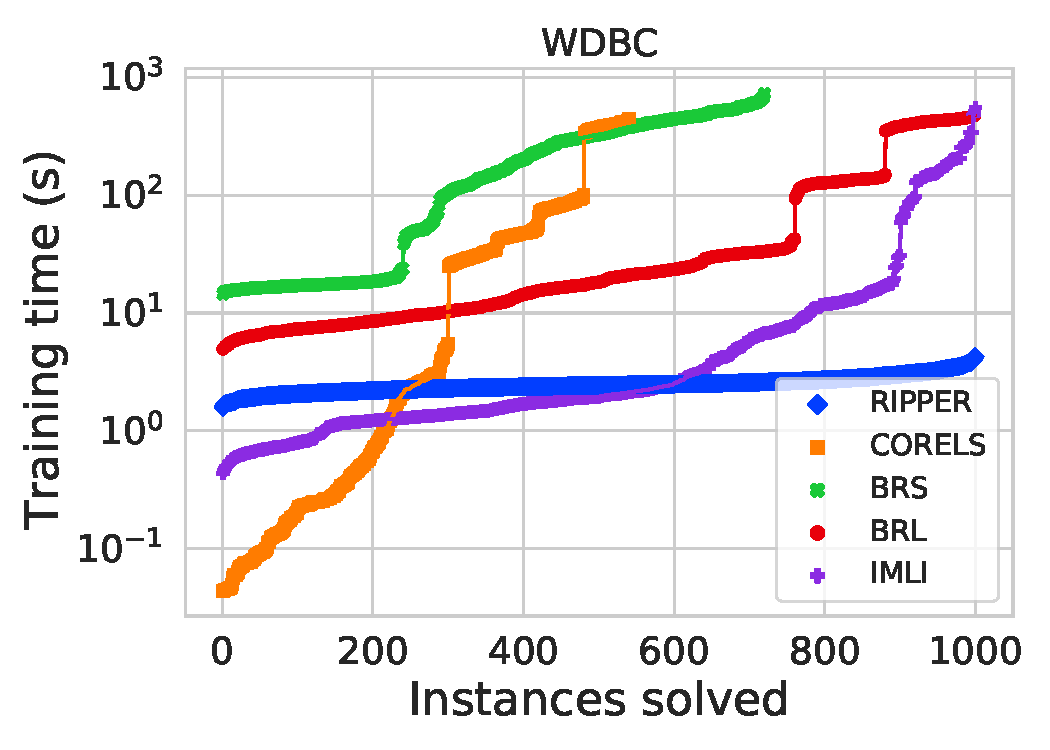
\includegraphics[scale=0.35]{figures/interpretability/imli/dataset_wdbc_cactus_train_val_fit_time}}
	\subfloat{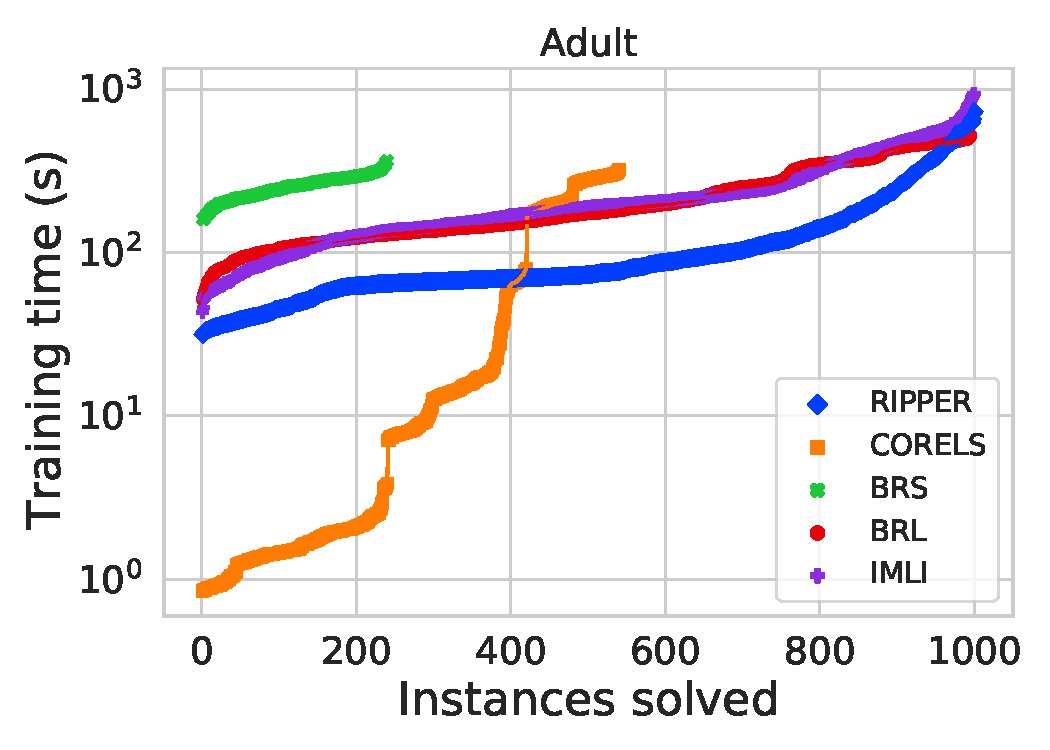
\includegraphics[scale=0.35]{figures/interpretability/imli/dataset_adult_cactus_train_val_fit_time}}\\
	\subfloat{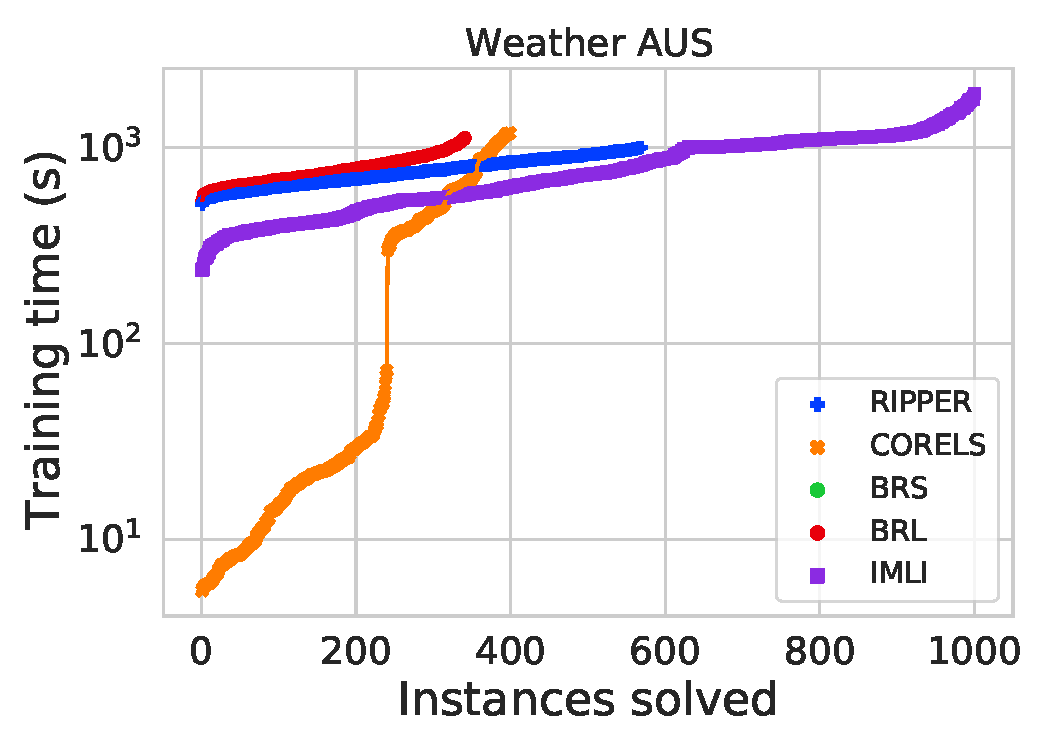
\includegraphics[scale=0.35]{figures/interpretability/imli/dataset_weatherAUS_cactus_train_val_fit_time}}
	\subfloat{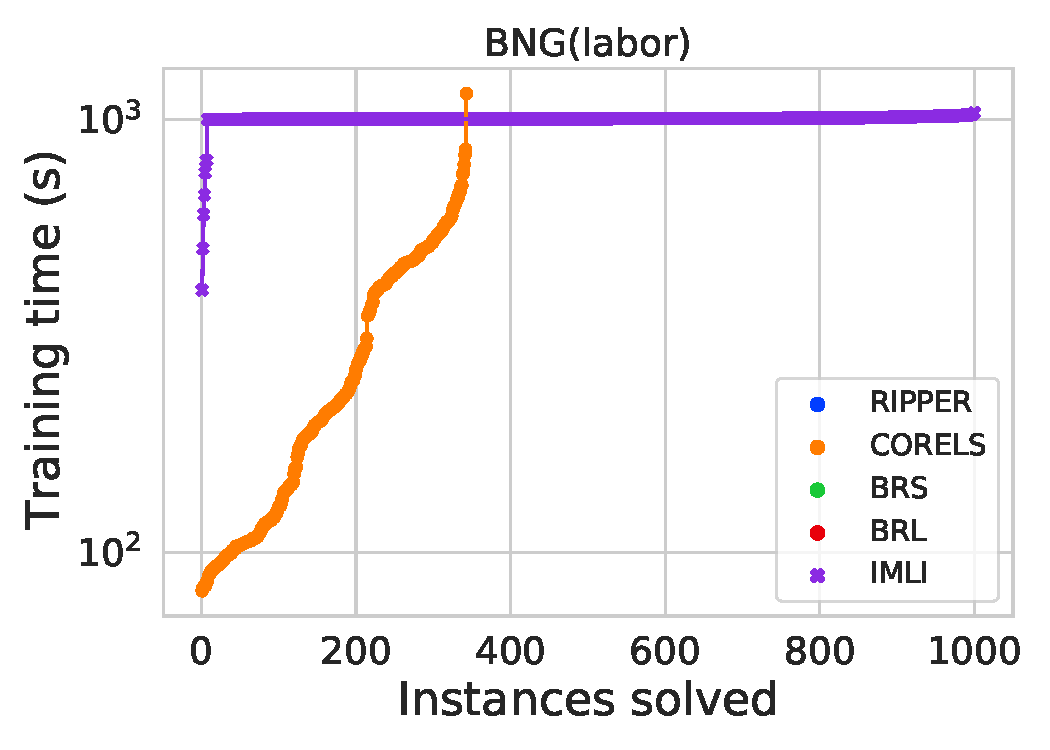
\includegraphics[scale=0.35]{figures/interpretability/imli/dataset_labor_cactus_train_val_fit_time}}
	
	\caption[Scalability of Interpretable Classifiers]{Comparison of scalability among interpretable classifiers. The plots are arranged in increasing sizes of datasets (from left to right). In each cactus plot, {\imli} solves all $ 1000 $ instances for each dataset, while competitive classifiers often fail to scale, specially in larger datasets.}
	\label{interpretability_imli_fig:interpretable_classifiers}
\end{figure}






\paragraph{Comparison with non-interpretable classifiers.} We compare {\imli} with state-of-the-art non-interpretable classifiers such as LR, SVM, kNN, and RF in terms of their median test accuracy in Table~\ref{interpretability_imli_table:non_interpretable_classifiers}. In the majority of the datasets, {\imli} achieves comparatively lower test accuracy than the best performing non-interpretable classifier. The decrease in the test accuracy of {\imli} is attributed to two factors. Firstly, while we train {\imli} on discretized data, non-interpretable classifiers are trained on non-discretized data and thus {\imli} incurs additional classification errors due to discretization. Secondly, {\imli} learns a rule-based classifier, whereas non-interpretable classifiers can learn more flexible decision boundaries and thus fit data well. In Table~\ref{interpretability_imli_table:non_interpretable_classifiers}, we also observe that {\imli} achieves impressive scalability than competing classifiers by solving datasets with $ 1, 000,000 $  samples where most of the non-interpretable classifiers fail to learn any decision boundary on such large datasets. Thus, {\imli}, being an interpretable classifier, demonstrates lower accuracy than competing non-interpretable classifiers, but higher scalability in practice. 


\begin{table*}[!t]        
	\centering
	\caption[Accuracy of {\imli} and non-interpretable classifiers]{Comparison of {\imli} with non-interpretable classifiers in terms of test accuracy. In the table, `\textemdash' represents a timeout. Numbers in bold represent the best performing results among different classifiers.}
	\label{interpretability_imli_table:non_interpretable_classifiers}
	%	\setlength{\tabcolsep}{.2em}
	\small
	\begin{tabular}{lrrrrrrrrrrrrrrr}
		
		
		
		
		\toprule
		Dataset & Size & LR & SVM & kNN & RF & IMLI \\
		
		\midrule
		\multirow{1}{*}{Parkinsons} & \multirow{1}{*}{ $ 195 $ }  &
		$ 89.74 $  &  $ 89.74 $  &  $ \mathbf{97.5} $  &  $ 90.0 $  &  $ 94.74 $  \\
		\multirow{1}{*}{WDBC} & \multirow{1}{*}{ $ 569 $ }  &
		$ \mathbf{98.25} $  &  $ \mathbf{98.25} $  &  $ 98.23 $  &  $ 96.49 $  &  $ 94.74 $  \\
		\multirow{1}{*}{Pima} & \multirow{1}{*}{ $ 768 $ }  &
		$ 78.43 $  &  $ 79.08 $  &  $ 74.5 $  &  $ \mathbf{79.22} $  &  $ 78.43 $  \\
		\multirow{1}{*}{Titanic} & \multirow{1}{*}{ $ 1,043 $ }  &
		$ 80.86 $  &  $ 80.38 $  &  $ 81.34 $  &  $ \mathbf{82.69} $  &  $ 81.82 $  \\
		\multirow{1}{*}{MAGIC} & \multirow{1}{*}{ $ 19,020 $ }  &
		$ 79.18 $  &  $ 79.34 $  &  $ 84.6 $  &  $ \mathbf{88.2} $  &  $ 78.26 $  \\
		\multirow{1}{*}{Tom's HW} & \multirow{1}{*}{ $ 28,179 $ }  &
		$ 96.2 $  &  $ 97.13 $  &  $ 88.15 $  &  $ \mathbf{97.78} $  &  $ 85.24 $  \\
		\multirow{1}{*}{Credit} & \multirow{1}{*}{ $ 30,000 $ }  &
		$ \mathbf{82.2} $  &  $ 81.9 $  &  $ 81.83 $  &  $ 82.15 $  &  $ 82.12 $  \\
		\multirow{1}{*}{Adult} & \multirow{1}{*}{ $ 32,561 $ }  &
		$ 85.26 $  &  $ 85.05 $  &  $ 83.8 $  &  $ \mathbf{86.69} $  &  $ 81.2 $  \\
		\multirow{1}{*}{Bank Marketing} & \multirow{1}{*}{ $ 45,211 $ }  &
		$ 90.09 $  &  $ 89.28 $  &  $ 89.43 $  &  $ \mathbf{90.27} $  &  $ 89.84 $  \\
		\multirow{1}{*}{Connect-4} & \multirow{1}{*}{ $ 67,557 $ }  &
		$ 79.39 $  & \textemdash &  $ 85.51 $  &  $ \mathbf{88.11} $  &  $ 75.36 $  \\
		\multirow{1}{*}{Weather AUS} & \multirow{1}{*}{ $ 107,696 $ }  &
		$ 85.64 $  & \textemdash &  $ 78.59 $  &  $ \mathbf{86.26} $  &  $ 83.78 $  \\
		\multirow{1}{*}{Vote} & \multirow{1}{*}{ $ 131,072 $ }  &
		$ 96.43 $  &  $ 96.37 $  &  $ 97.05 $  &  $ \mathbf{97.38} $  &  $ 96.69 $  \\
		\multirow{1}{*}{Skin Seg} & \multirow{1}{*}{ $ 245,057 $ }  &
		$ 91.86 $  & \textemdash &  $ \mathbf{99.96} $  &  $ \mathbf{99.96} $  &  $ 94.71 $  \\
		\multirow{1}{*}{BNG(labor)} & \multirow{1}{*}{ $ 1,000,000 $ }  &
		\textemdash & \textemdash & \textemdash & \textemdash &  $ \mathbf{90.91} $  \\
		\multirow{1}{*}{BNG(credit-g)} & \multirow{1}{*}{ $ 1,000,000 $ }  &
		\textemdash & \textemdash & \textemdash &  $ \mathbf{80.58} $  &  $ 75.48 $  \\
		\bottomrule
		
		
		
	\end{tabular}
	
\end{table*}


\begin{figure}[!t]
	
	
	\centering
	
	\subfloat{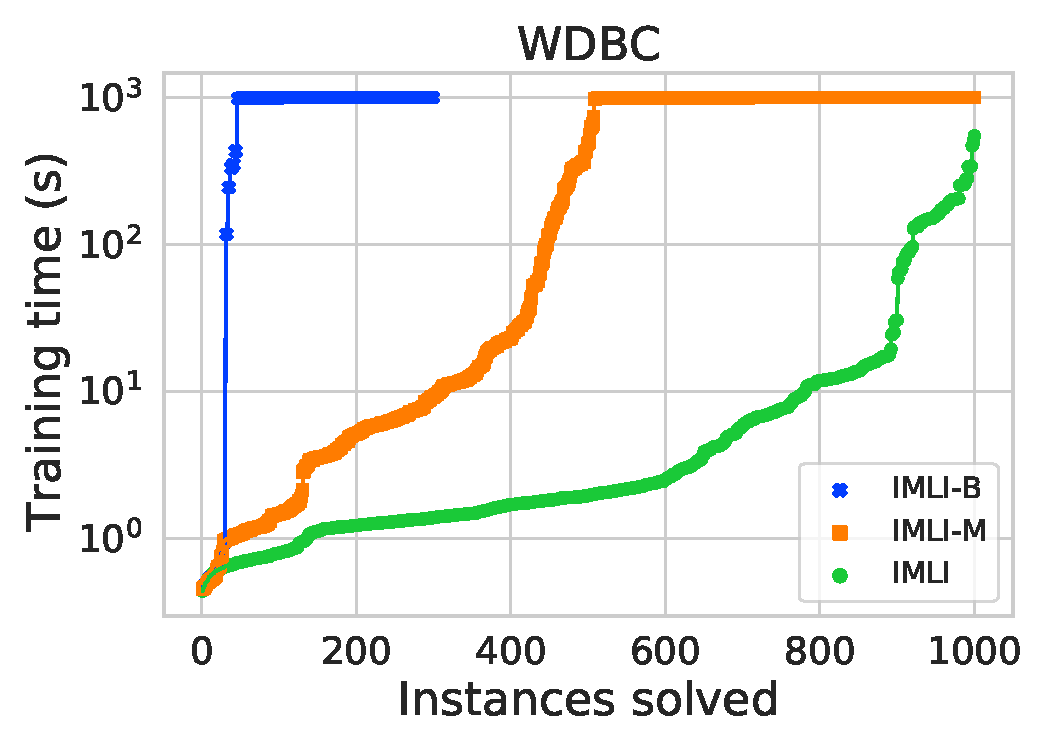
\includegraphics[scale=0.3]{figures/interpretability/imli/imli_exp_wdbc_cactus_train_val_fit_time}}	
	\subfloat{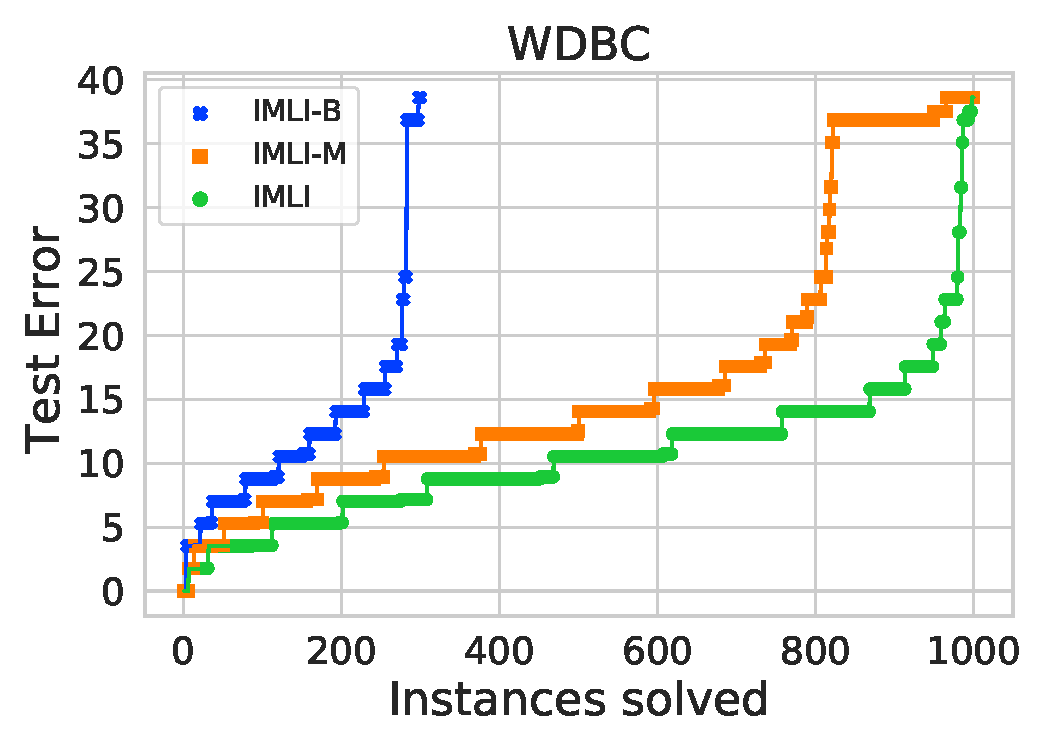
\includegraphics[scale=0.3]{figures/interpretability/imli/imli_exp_wdbc_cactus_test_accuracy}}
	\subfloat{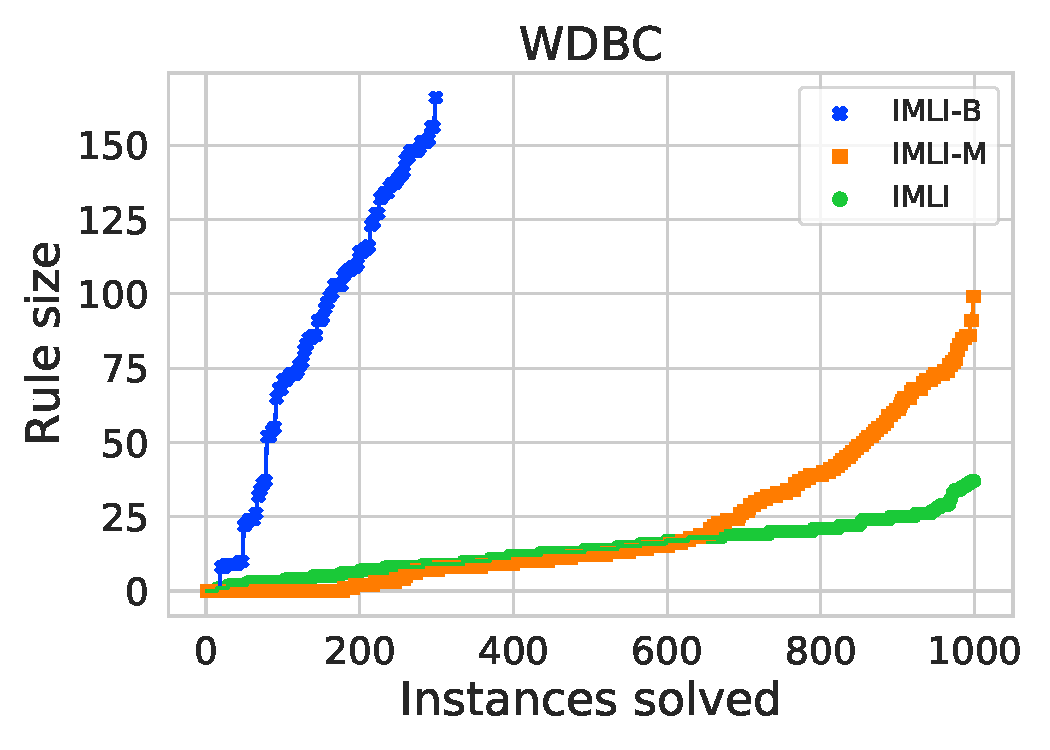
\includegraphics[scale=0.3]{figures/interpretability/imli/imli_exp_wdbc_cactus_predicate_count}}
		
	
	\subfloat{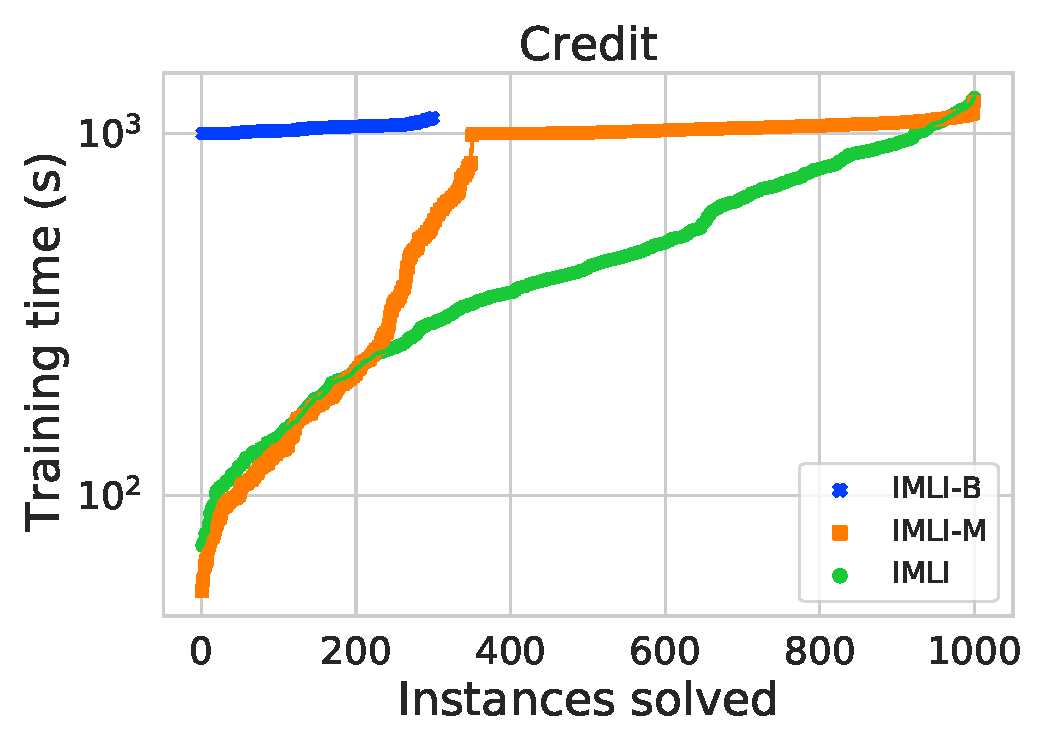
\includegraphics[scale=0.3]{figures/interpretability/imli/imli_exp_credit_cactus_train_val_fit_time}}	
	\subfloat{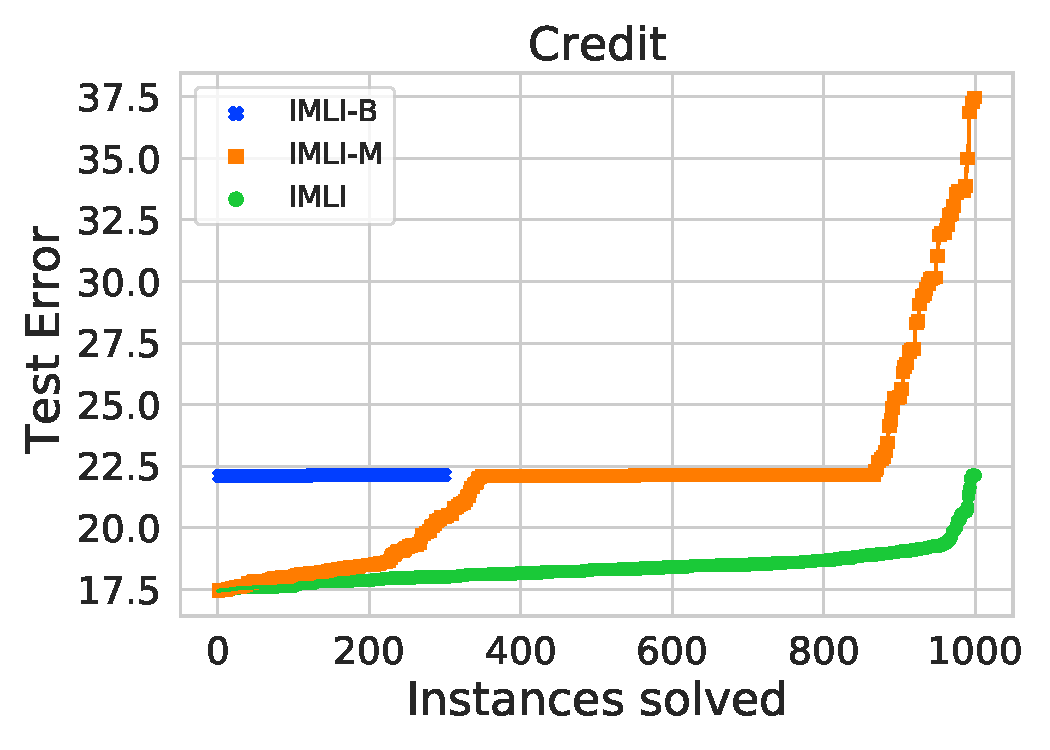
\includegraphics[scale=0.3]{figures/interpretability/imli/imli_exp_credit_cactus_test_accuracy}}
	\subfloat{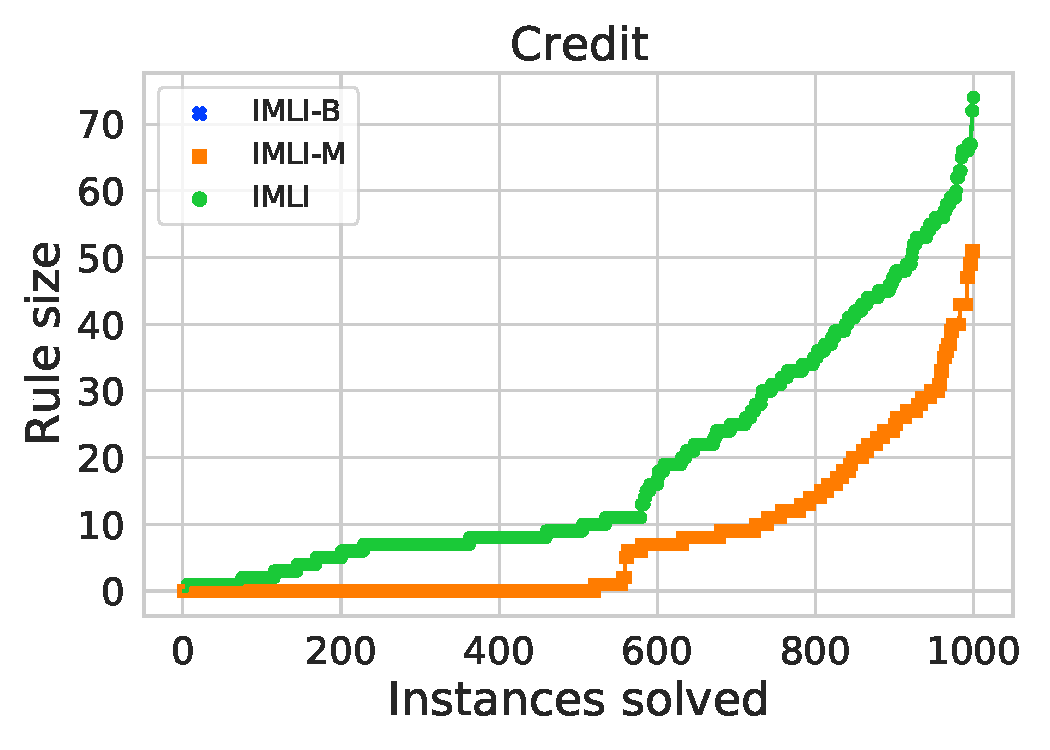
\includegraphics[scale=0.3]{figures/interpretability/imli/imli_exp_credit_cactus_predicate_count}}
	

	\subfloat{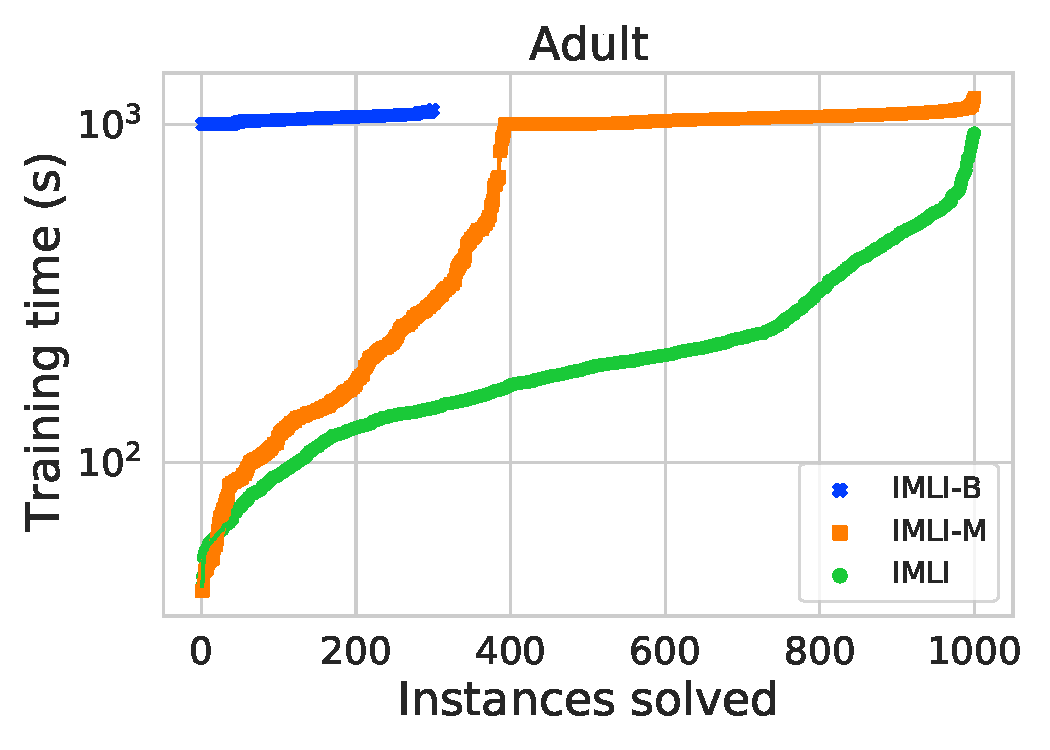
\includegraphics[scale=0.3]{figures/interpretability/imli/imli_exp_adult_cactus_train_val_fit_time}}	
	\subfloat{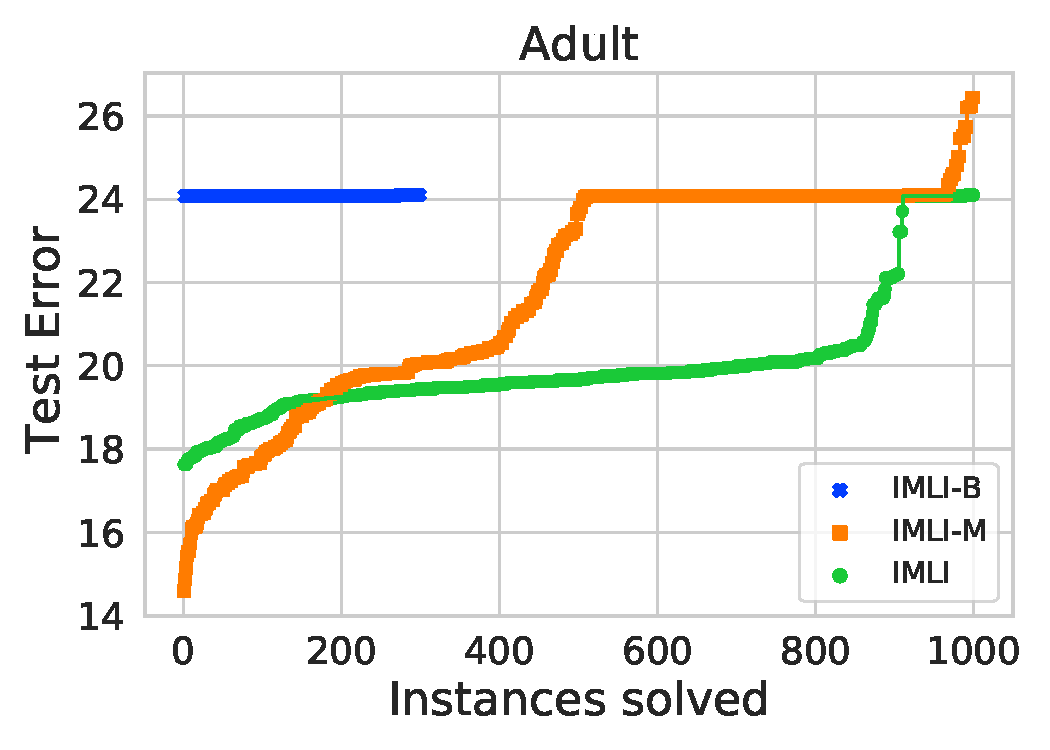
\includegraphics[scale=0.3]{figures/interpretability/imli/imli_exp_adult_cactus_test_accuracy}}
	\subfloat{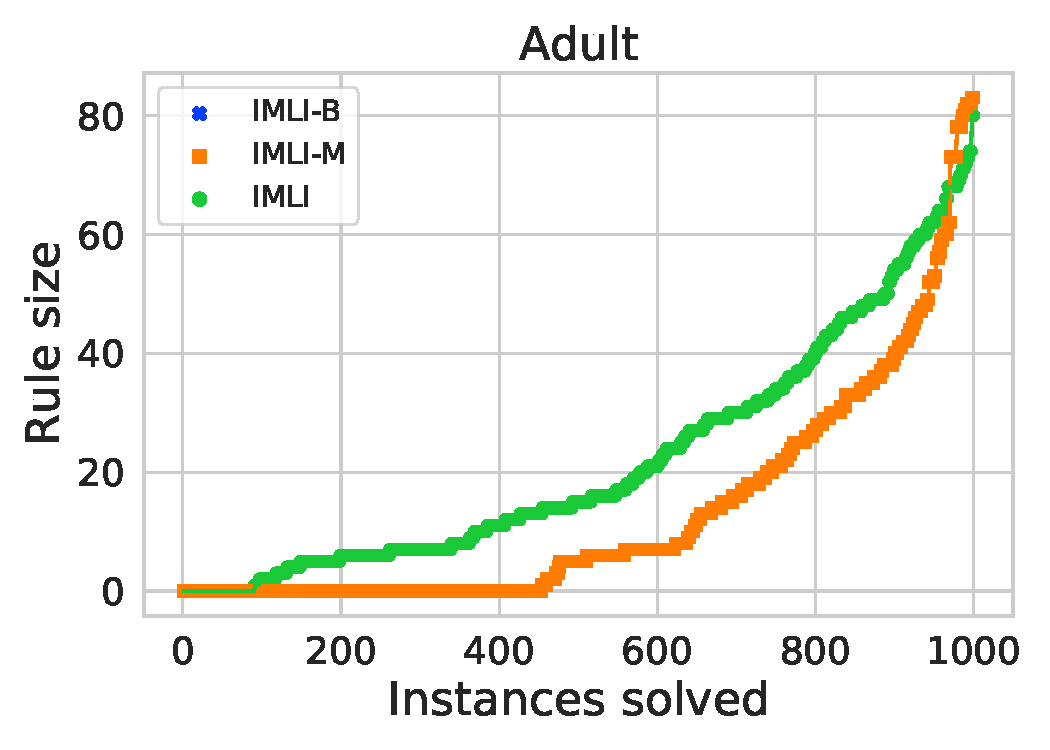
\includegraphics[scale=0.3]{figures/interpretability/imli/imli_exp_adult_cactus_predicate_count}}

	
	\caption[Training time, test error, and rule-size of different formulations in {\imli}]{Comparison of training time, test error, and rule-size among different formulations presented in the chapter. In each cactus plot, the incremental formulation {\imli} with both mini-batch and iterative learning demonstrates the best performance in training time and test error than compared two formulations: non-incremental MaxSAT formulation {\imli}-$\mathsf{B}$ and incremental formulation with only mini-batch learning {\imli}-$\mathsf{M}$. In terms of rule-size, {\imli} often generates higher size rules than {\imli}-$\mathsf{M}$.}
	\label{interpretability_imli_fig:different_formulations}
\end{figure}



\paragraph{Comparison among different formulations in {\imli}.}  We compare the performance of different formulations for learning classification rules as presented in this chapter. In Figure~\ref{interpretability_imli_fig:different_formulations}, we show cactus plots for assessing training time (in seconds), test error (in percentage), and rule-size among different formulations. In the cactus plot, a point $ (x,y) $ denotes that the formulation yields lower than or equal to $ y $ training time (similarly, test error and rule-size) in $ x $ many instances in each dataset.

In Figure~\ref{interpretability_imli_fig:different_formulations}, we denote the baseline non-incremental MaxSAT-based formulation as {\imli}-$\mathsf{B}$\footnote{Since  {\imli}-$\mathsf{B}$ is a non-incremental formulation and does not involve any mini-batch learning, we consider two hyper-parameters for {\imli}-$\mathsf{B}$: the number of clauses in $ \{1, 2, \dots, 10\} $ and the regularization parameter $ \lambda $ as $ 10 $ values chosen from a logarithmic grid between $ 10^{-4} $ and $ 10^1 $.}, incremental MaxSAT-based formulation with only mini-batch learning as {\imli}-$\mathsf{M}$, and incremental MaxSAT-based formulation with both mini-batch and iterative learning as {\imli}.  We first observe the training time of different formulations in the left-most column in Figure~\ref{interpretability_imli_fig:different_formulations}, where {\imli}-$\mathsf{B}$ soon times out and solves lower than $ 300 $ instances out of $ 1000 $ instances in each dataset. This result suggests that the non-incremental formulation cannot scale in practical classification task. Comparing between {\imli} and {\imli}-$\mathsf{M}$, both formulations solve all $ 1000 $ instances in each dataset with {\imli}-$\mathsf{M}$ undertaking significantly higher training time than $ {\imli} $.  Therefore, {\imli} achieves better scalability than {\imli}-$\mathsf{M}$ indicating that an integration of mini-batch and iterative learning achieves a significant progress in terms of scalability than mini-batch learning alone. 

We next focus on the test error of different formulations in the middle column in Figure~\ref{interpretability_imli_fig:different_formulations}. Firstly, {\imli}-$\mathsf{B}$ has a higher test error than the other two formulations since {\imli}-$\mathsf{B}$ times out in most instances and learns a sub-optimal classification rule with reduced prediction accuracy. In contrast, {\imli} has the lowest test error compared to two formulations in all datasets. This result indicates the effectiveness of integrating both iterative and mini-batch learning with MaxSAT-based formulation in generating more accurate classification rules.


Moving focus on the rule-size in the rightmost column in Figure~\ref{interpretability_imli_fig:different_formulations}, {\imli}-$\mathsf{B}$ achieves the highest rule-size in WDBC dataset. In contrast, the rule-size of {\imli}-$\mathsf{B}$  is lowest (zero) in Credit and Adult datasets. In the last two datasets, {\imli}-$\mathsf{B}$ times out during training and returns the default rule ``true'' by predicting all samples as class $ 1 $. The other two formulations {\imli} and {\imli}-$\mathsf{M}$  demonstrate a similar trend in rule-size in all datasets with {\imli}-$\mathsf{M}$ generating comparatively smaller size rules in Credit and Adult datasets. In this context,  the improvement of rule-sparsity of {\imli}-$\mathsf{M}$ is due to a comparatively higher test error (or lower accuracy) than {\imli} as observed in all three datasets. Therefore, {\imli} appears to be the best performing formulation w.r.t.\ training time, test error, and rule-size by balancing between accuracy and rule-size while being more scalable.

\begin{table*}[!t]        
	\centering
	\caption[Accuracy and rule-size of different classification rules learned using {\imli}]{Comparison of test accuracy (top value) and rule-size (bottom value) among different rule-based representations learned using {\imli}. Numbers in bold denote the best performing results among different representations.}
	\label{interpretability_imli_table:different_representations}
	%	\setlength{\tabcolsep}{.2em}
	\small
	\begin{tabular}{lrrrrrrrrrrrrrrr}
		
		
		
		


\toprule
Dataset & CNF & DNF & Decision Sets & Decision Lists \\

\midrule
\multirow{2}{*}{Parkinsons}  &
$ 94.74 $  &  $ 89.47 $  &  $ \mathbf{94.87} $  &  $ 89.74 $  \\
& $ 7.5 $  &  $ \mathbf{6.0} $  &  $ 15.0 $  &  $ 6.5 $  \\
\addlinespace[0.5em]

\multirow{2}{*}{WDBC}  &
$ 94.74 $  &  $ \mathbf{96.49} $  &  $ 95.61 $  &  $ 95.61 $  \\
& $ 11.5 $  &  $ 15.0 $  &  $ 15.5 $  &  $ \mathbf{10.0} $  \\
\addlinespace[0.5em]

\multirow{2}{*}{Pima}  &
$ \mathbf{78.43} $  &  $ 77.13 $  &  $ 76.97 $  &  $ 76.97 $  \\
& $ 23.0 $  &  $ \mathbf{9.0} $  &  $ 15.0 $  &  $ 13.5 $  \\
\addlinespace[0.5em]

\multirow{2}{*}{Titanic}  &
$ 81.82 $  &  $ 82.29 $  &  $ 81.82 $  &  $ \mathbf{82.3} $  \\
& $ \mathbf{5.5} $  &  $ 10.5 $  &  $ 8.5 $  &  $ 8.0 $  \\
\addlinespace[0.5em]

\multirow{2}{*}{MAGIC}  &
$ \mathbf{78.26} $  &  $ 77.44 $  &  $ 75.87 $  &  $ 77.79 $  \\
& $ \mathbf{8.5} $  &  $ 41.5 $  &  $ 10.0 $  &  $ 14.0 $  \\
\addlinespace[0.5em]

\multirow{2}{*}{Tom's HW}  &
$ 85.24 $  &  $ 85.15 $  &  $ 85.72 $  &  $ \mathbf{85.95} $  \\
& $ 44.5 $  &  $ \mathbf{26.5} $  &  $ 45.0 $  &  $ 59.5 $  \\
\addlinespace[0.5em]

\multirow{2}{*}{Credit}  &
$ 82.12 $  &  $ 82.15 $  &  $ 82.03 $  &  $ \mathbf{82.22} $  \\
& $ 17.5 $  &  $ 14.0 $  &  $ \mathbf{9.5} $  &  $ 21.5 $  \\
\addlinespace[0.5em]

\multirow{2}{*}{Adult}  &
$ 81.2 $  &  $ \mathbf{84.28} $  &  $ 80.07 $  &  $ 80.96 $  \\
& $ 30.0 $  &  $ 34.5 $  &  $ \mathbf{7.0} $  &  $ 24.5 $  \\
\addlinespace[0.5em]

\multirow{2}{*}{Bank Marketing}  &
$ \mathbf{89.84} $  &  $ 89.77 $  &  $ 89.67 $  &  $ 89.79 $  \\
& $ 24.5 $  &  $ 7.5 $  &  $ \mathbf{6.0} $  &  $ 10.5 $  \\
\addlinespace[0.5em]

\multirow{2}{*}{Connect-4}  &
$ \mathbf{75.36} $  &  $ 70.63 $  &  $ 68.09 $  &  $ 69.83 $  \\
& $ 50.5 $  &  $ 42.0 $  &  $ \mathbf{4.5} $  &  $ 24.0 $  \\
\addlinespace[0.5em]

\multirow{2}{*}{Weather AUS}  &
$ 83.78 $  &  $ \mathbf{84.23} $  &  $ 83.69 $  &  $ 83.85 $  \\
& $ 22.0 $  &  $ 14.0 $  &  $ \mathbf{4.0} $  &  $ 26.0 $  \\
\addlinespace[0.5em]


\multirow{2}{*}{Skin Seg}  &
$ \mathbf{94.71} $  &  $ 93.68 $  &  $ 87.92 $  &  $ 91.17 $  \\
& $ 30.0 $  &  $ 15.0 $  &  $ \mathbf{3.0} $  &  $ 7.0 $  \\
\bottomrule

	
				
	\end{tabular}
	
\end{table*}




\paragraph{Performance evaluation of different interpretable representations in {\imli}.}

We deploy {\imli} to learn different interpretable rule-based representations: CNF and DNF classifiers, decision lists, and decision sets and present their comparative performance w.r.t.\ test accuracy and rule-size in Table~\ref{interpretability_imli_table:different_representations}. In each cell in this table, the top value represents the test accuracy and the bottom value represents the size of generated rules.


We learn all four interpretable representations on twelve datasets, where the CNF classifier appears to be the most accurate representation by achieving the highest accuracy in five datasets. In contrast, both DNF and decision lists achieve the highest accuracy in three datasets each; decision sets demonstrate the least performance in test accuracy by being more accurate in one dataset. To this end, the poor accuracy of decision sets is traded off by its rule-size as decision sets generate the sparsest rules compared to other representations. More precisely, decision sets have the smallest rule-size in six datasets, while CNF, DNF, and decision lists have the smallest rule-size in two, three, and one dataset, respectively. These results suggest that CNF classifiers are more favored in applications where higher accuracy is preferred, while decision sets are preferred in applications where higher interpretability is desired. In both cases, one could deploy {\imli} for learning varied representations of classification rules. 




\begin{figure}[!t]
	
	\centering
	
	\subfloat{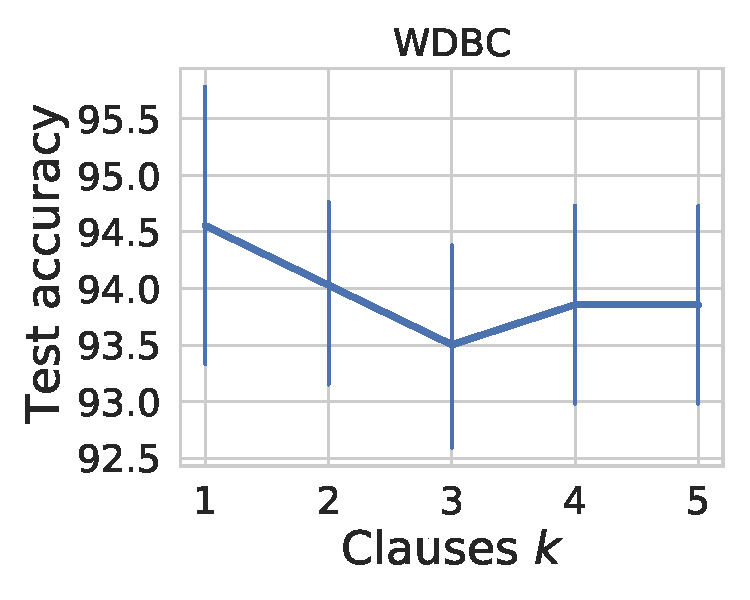
\includegraphics[scale=0.3]{figures/interpretability/imli/clauses_test_accuracy_wdbc}}
	\subfloat{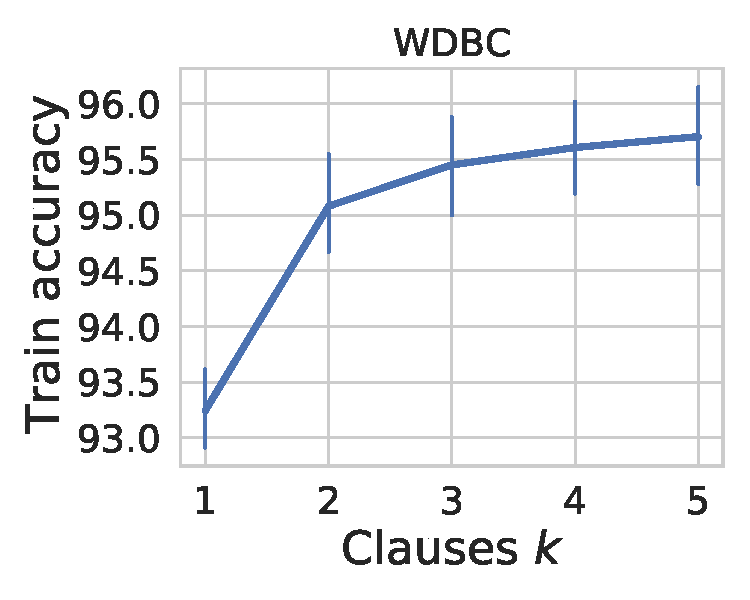
\includegraphics[scale=0.3]{figures/interpretability/imli/clauses_train_val_accuracy_wdbc}}
	\subfloat{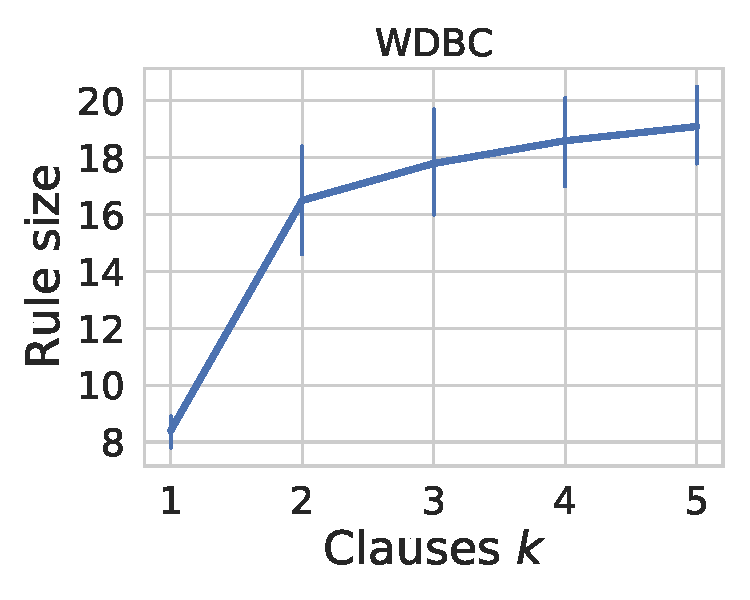
\includegraphics[scale=0.3]{figures/interpretability/imli/clauses_predicate_count_wdbc}}
	\subfloat{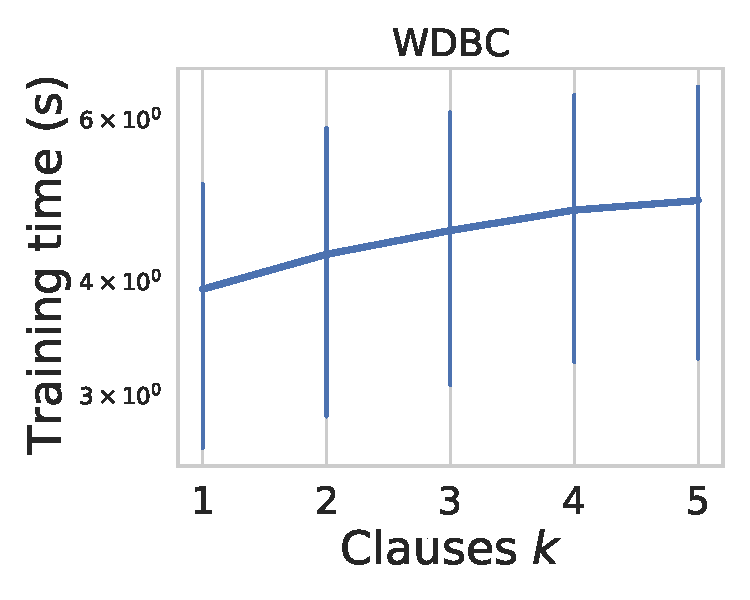
\includegraphics[scale=0.3]{figures/interpretability/imli/clauses_train_val_fit_time_wdbc}}
	
	
	\subfloat{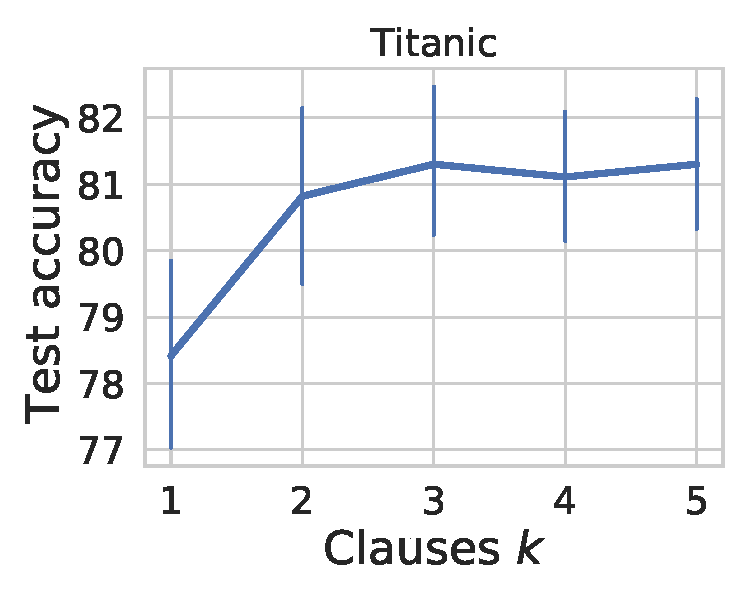
\includegraphics[scale=0.3]{figures/interpretability/imli/clauses_test_accuracy_titanic}}
	\subfloat{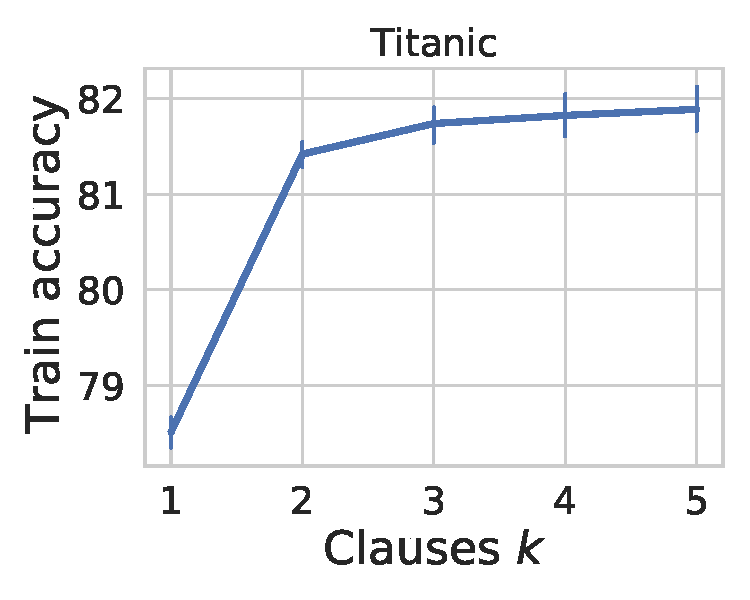
\includegraphics[scale=0.3]{figures/interpretability/imli/clauses_train_val_accuracy_titanic}}
	\subfloat{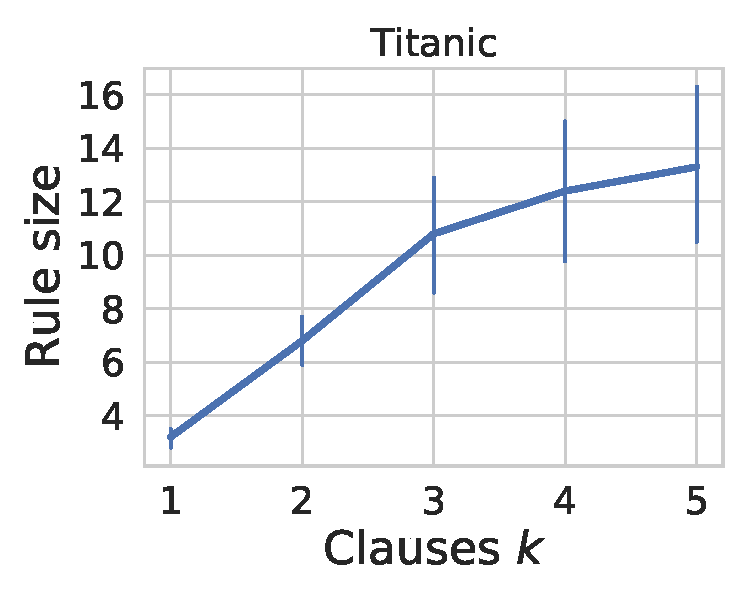
\includegraphics[scale=0.3]{figures/interpretability/imli/clauses_predicate_count_titanic}}
	\subfloat{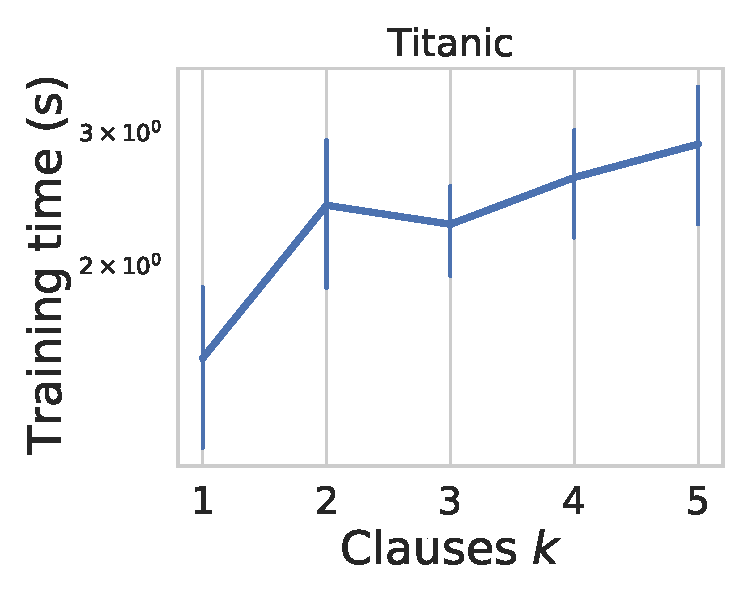
\includegraphics[scale=0.3]{figures/interpretability/imli/clauses_train_val_fit_time_titanic}}
	
	
	\subfloat{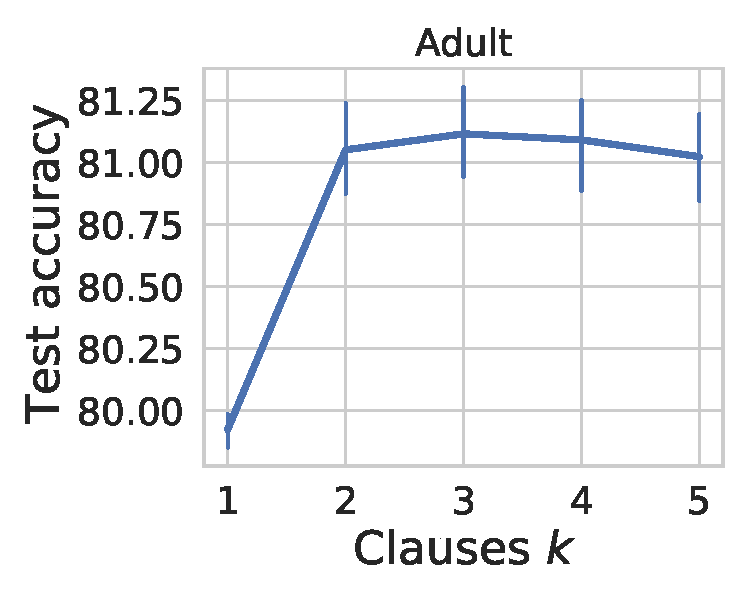
\includegraphics[scale=0.3]{figures/interpretability/imli/clauses_test_accuracy_adult}}
	\subfloat{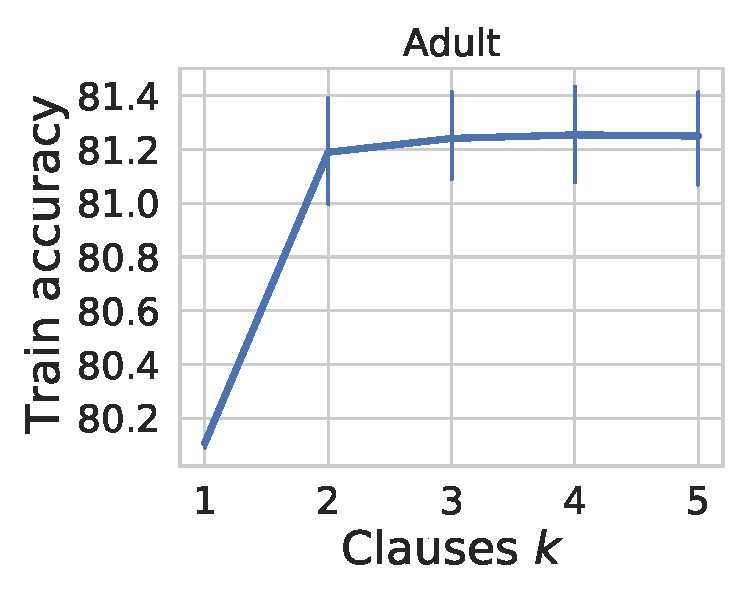
\includegraphics[scale=0.3]{figures/interpretability/imli/clauses_train_val_accuracy_adult}}
	\subfloat{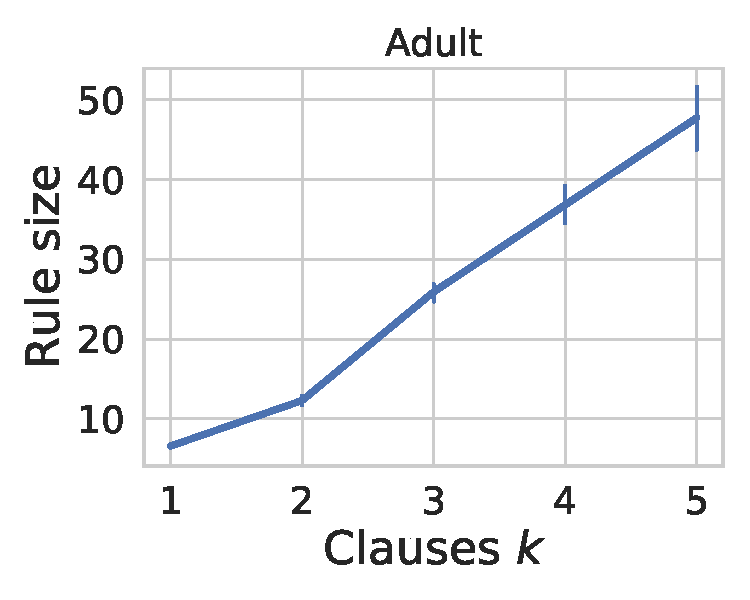
\includegraphics[scale=0.3]{figures/interpretability/imli/clauses_predicate_count_adult}}
	\subfloat{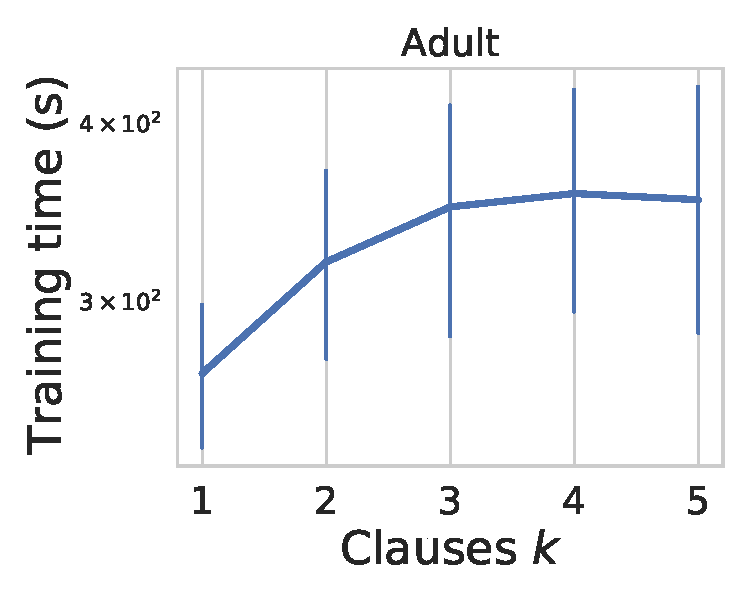
\includegraphics[scale=0.3]{figures/interpretability/imli/clauses_train_val_fit_time_adult}}
	
	
	
	
	\caption[Effect of the number of clauses in {\imli}]{Effect of the number of clauses $ k $ on accuracy (test and train), rule-size, and training time. As $ k $ increases, both train and test accuracy of {\imli} increase while generating rules with higher size by incurring higher training time. }
	\label{interpretability_imli_fig:effect_of_number_of_clauses}
\end{figure}

\paragraph{Ablation study.} We experiment the effect of different hyper-parameters in {\imli} on prediction accuracy, rule-size, and training time in different datasets. In the following, we discuss the impact of the number of clauses, regularization parameter, and size of mini-batches in {\imli}.


\textbf{Effect of the number of clauses $ k $.} In Figure~\ref{interpretability_imli_fig:effect_of_number_of_clauses}, we vary  $ k $ while learning CNF classifiers in {\imli}. As $ k $ increases, both training and test accuracy generally increase in different datasets (plots in the first and second columns). Similarly, the size of rules increases with $ k $ by incurring higher training time (plots in the third and fourth columns). The reason is that a higher value of $ k $ allows more flexibility in fitting the data well by incurring more training time and generating higher size classification rules. Therefore, the number of clauses in {\imli} provides control on training-time vs accuracy and also on accuracy vs rule-sparsity. 


\textbf{Effect of regularizer $ \lambda $.} In Figure~\ref{interpretability_imli_fig:effect_of_number_of_regularization}, we vary $ \lambda $ in a logarithmic grid between $ 10^{-4} $ and $ 10^1 $. As stated in Eq.~\eqref{interpretability_imli_eq:obj_incr}, a higher value of $ \lambda $ puts more priority on the minimal changes in rules between consecutive mini-batches in incremental learning while allowing higher mini-batch errors. Thus, in the first and second columns in Figure~\ref{interpretability_imli_fig:effect_of_number_of_regularization}, as $ \lambda $ increases, both training and test accuracy gradually decrease. In addition, the size of rules (plots in the third column) also decreases. Finally, we observe that the training time generally decreases with $ \lambda $. This observation indicates that higher $ \lambda $ puts lower computational load to the MaxSAT solver as a fraction of training examples is allowed to be misclassified. Thus, similar to the number of clauses, regularization parameter $ \lambda $ in {\imli} allows to trade-off between accuracy and rule-size in a precise manner.

\textbf{Effect of the size of mini-batch.} In Figure~\ref{interpretability_imli_fig:effect_of_batch_size}, we present the effect of mini-batch size in {\imli}. As we consider more samples in a batch, both test and training accuracy increase in general as presented in the first and second columns in Figure~\ref{interpretability_imli_fig:effect_of_batch_size}. Similarly, the size of generated rules also increases with the number of samples. Due to solving higher size MaxSAT queries, the training time also increases in general with an increase in mini-batch size. Therefore, by varying the size of mini-batches, {\imli} allows controlling on training time vs the prediction accuracy (and rule-size) of generated rules. 


\begin{figure}[!t]
	
	\centering
	
	
	\subfloat{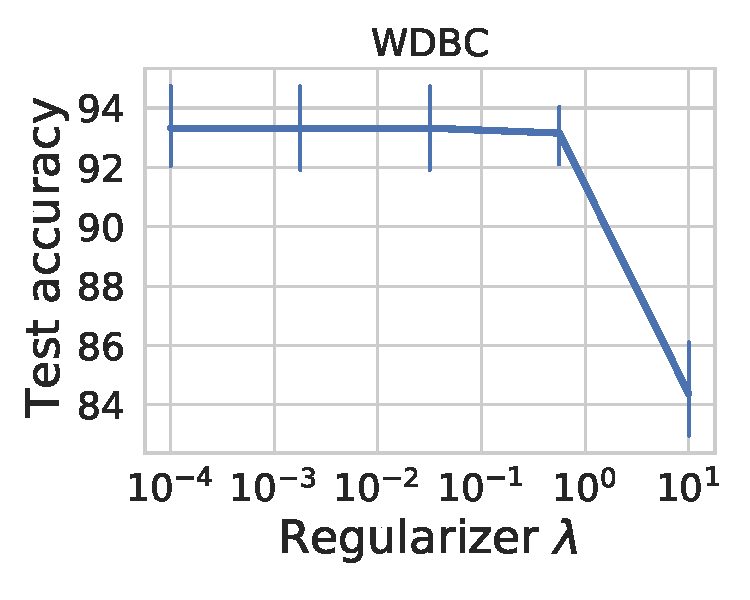
\includegraphics[scale=0.3]{figures/interpretability/imli/lambda__test_accuracy_wdbc}}
	\subfloat{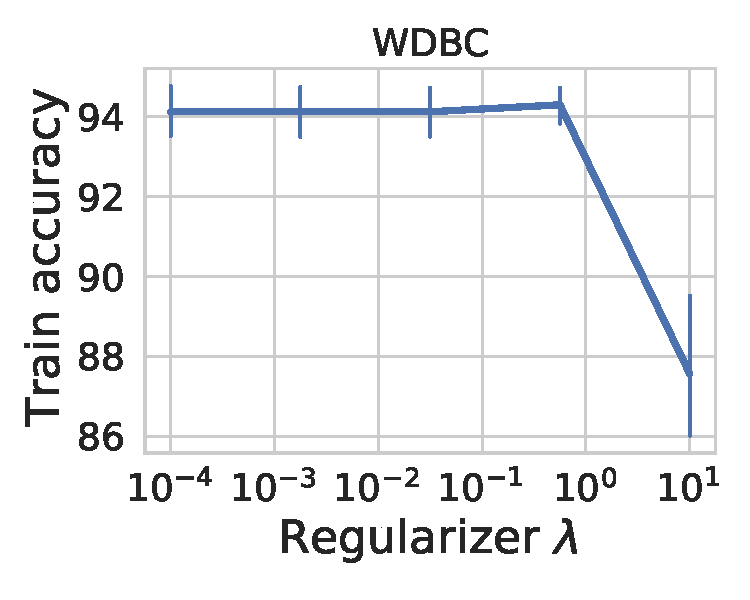
\includegraphics[scale=0.3]{figures/interpretability/imli/lambda__train_val_accuracy_wdbc}}
	\subfloat{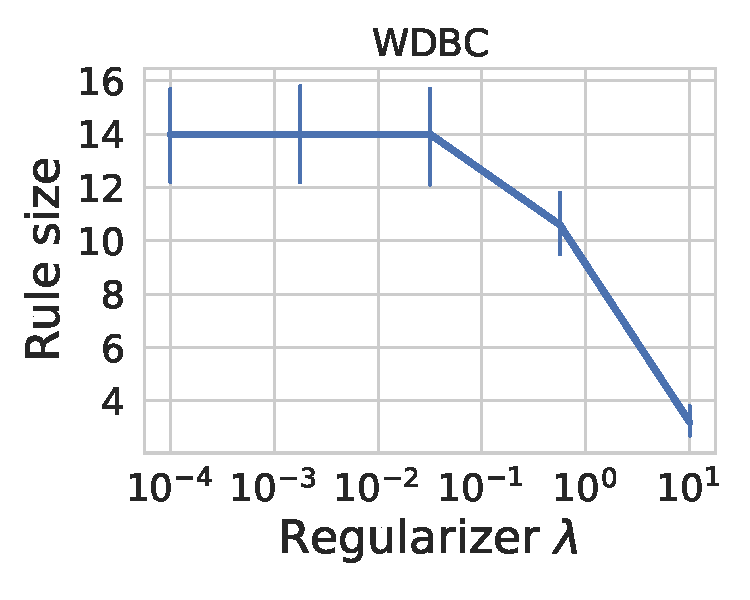
\includegraphics[scale=0.3]{figures/interpretability/imli/lambda__predicate_count_wdbc}}
	\subfloat{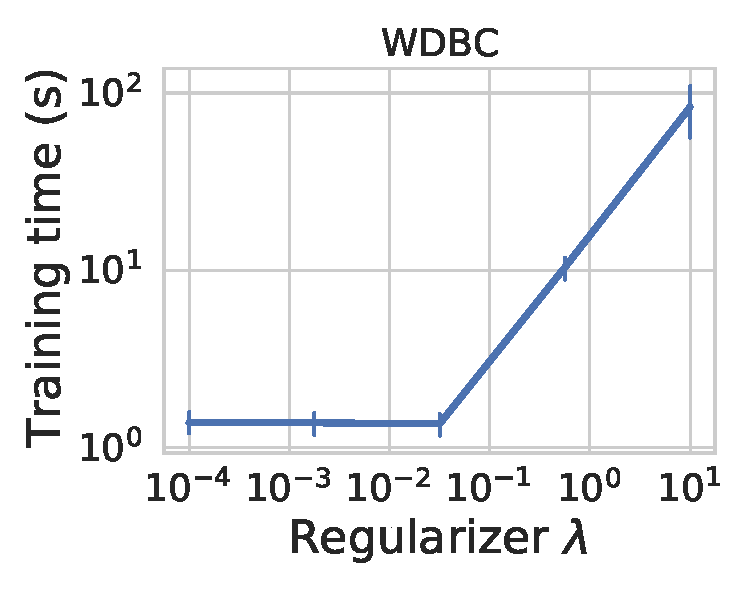
\includegraphics[scale=0.3]{figures/interpretability/imli/lambda__train_val_fit_time_wdbc}}


	\subfloat{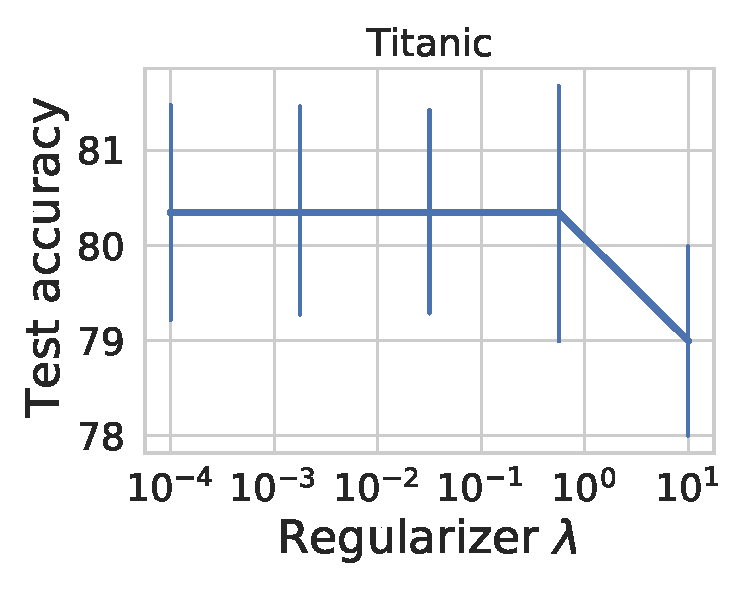
\includegraphics[scale=0.3]{figures/interpretability/imli/lambda__test_accuracy_titanic}}
	\subfloat{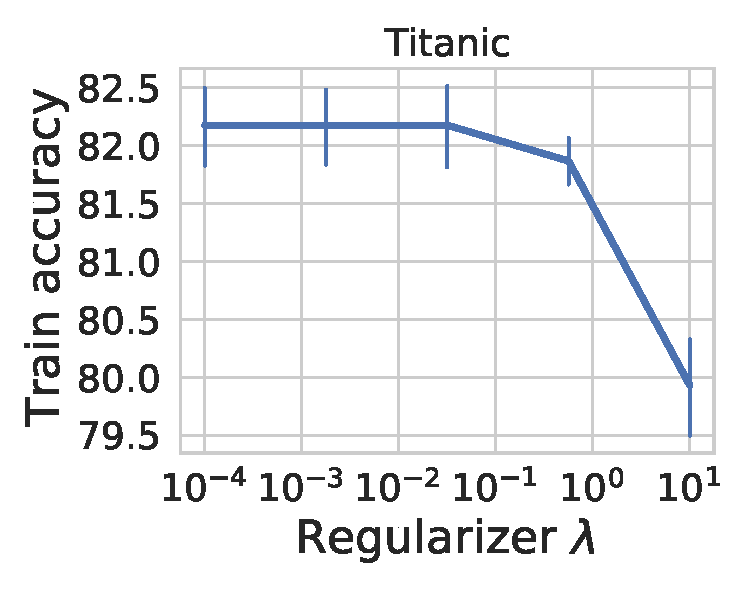
\includegraphics[scale=0.3]{figures/interpretability/imli/lambda__train_val_accuracy_titanic}}
	\subfloat{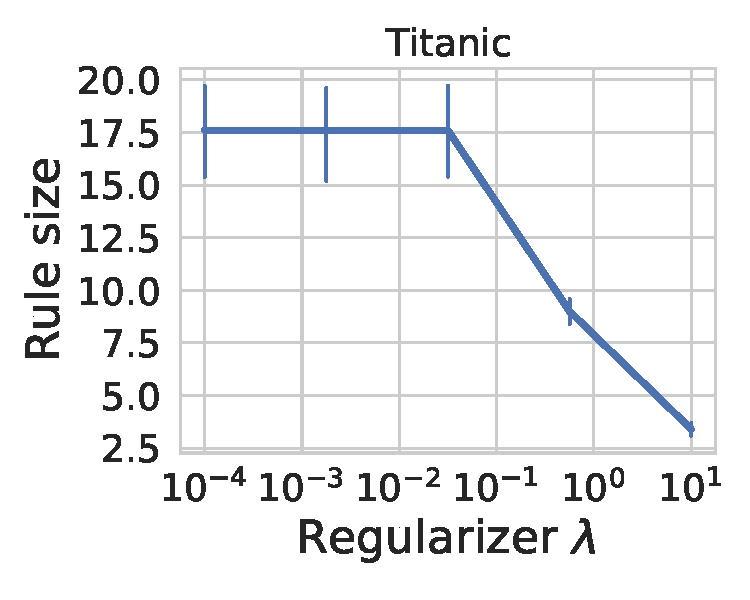
\includegraphics[scale=0.3]{figures/interpretability/imli/lambda__predicate_count_titanic}}
	\subfloat{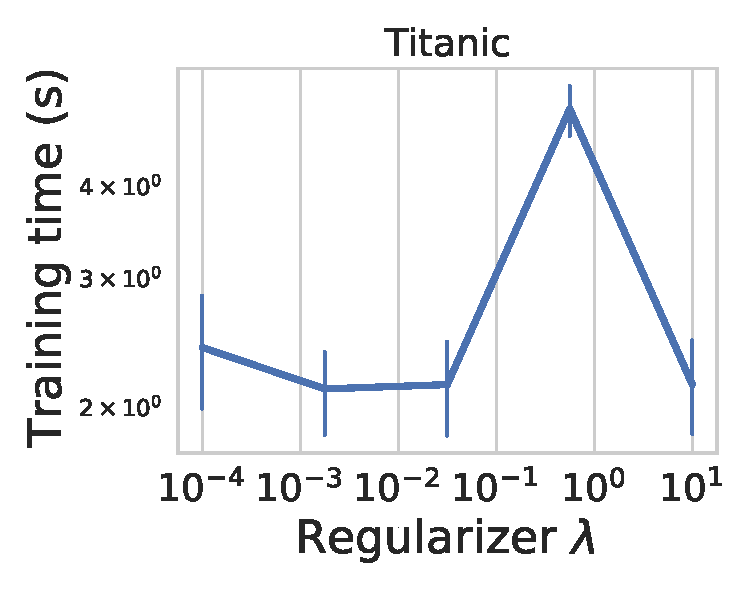
\includegraphics[scale=0.3]{figures/interpretability/imli/lambda__train_val_fit_time_titanic}}	
	
	\subfloat{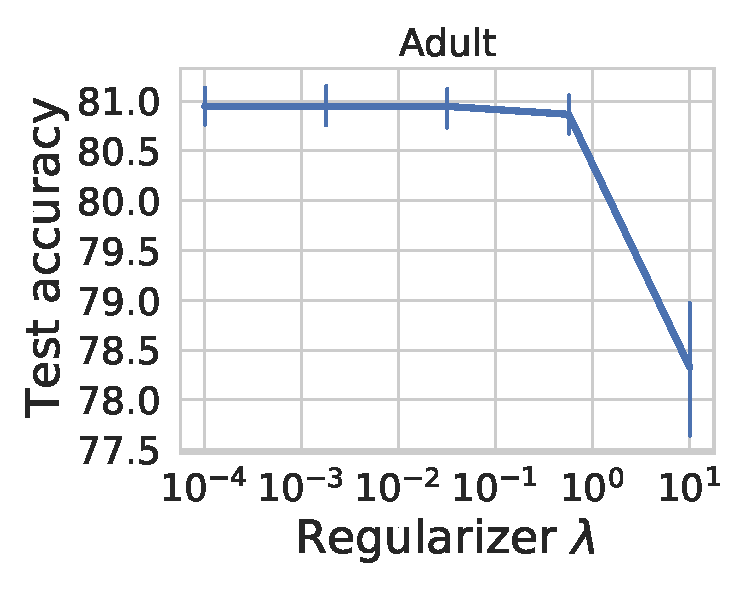
\includegraphics[scale=0.3]{figures/interpretability/imli/lambda__test_accuracy_adult}}
	\subfloat{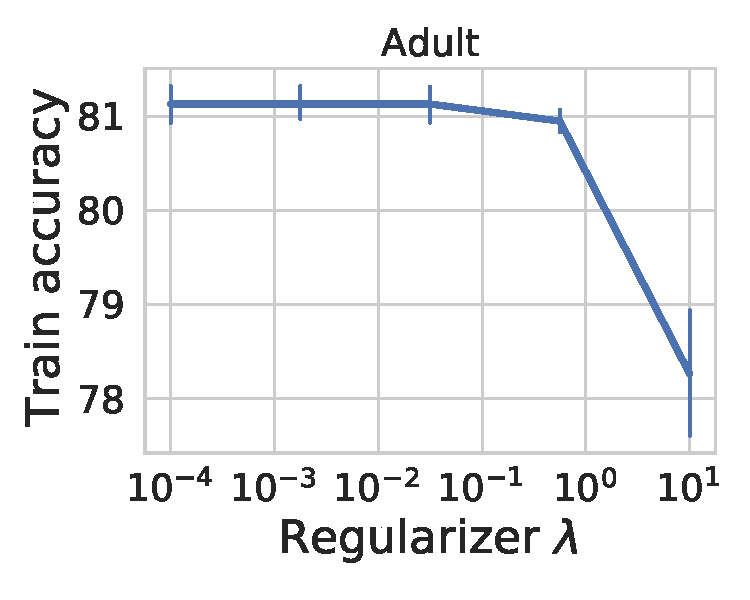
\includegraphics[scale=0.3]{figures/interpretability/imli/lambda__train_val_accuracy_adult}}
	\subfloat{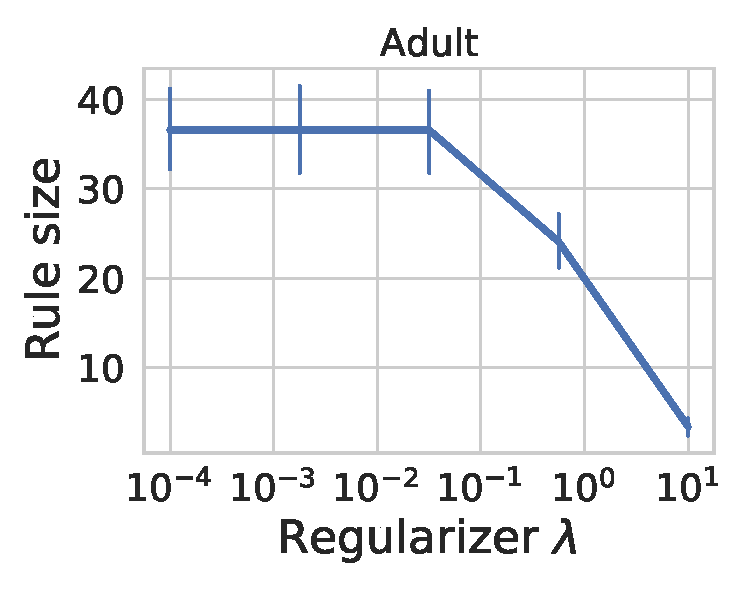
\includegraphics[scale=0.3]{figures/interpretability/imli/lambda__predicate_count_adult}}
	\subfloat{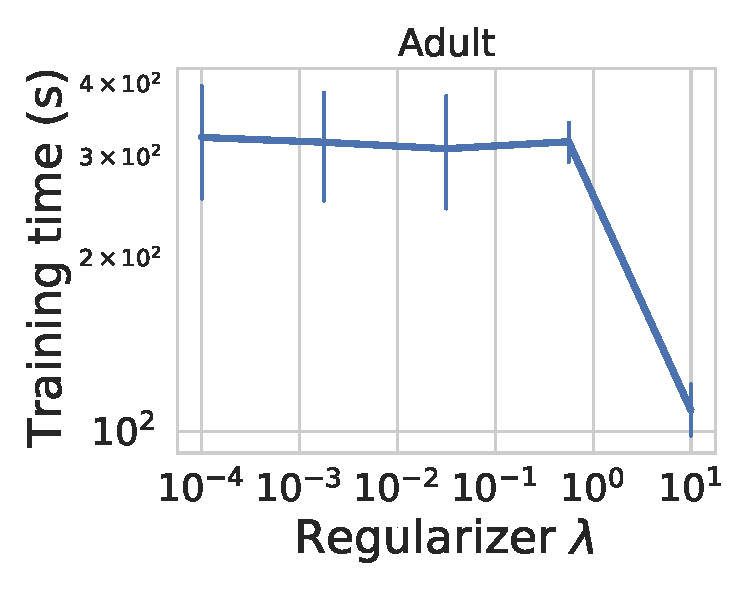
\includegraphics[scale=0.3]{figures/interpretability/imli/lambda__train_val_fit_time_adult}}
	
	
	
	
	
	\caption[Effect of regularization $ \lambda $ in {\imli}]{Effect of regularization $ \lambda $ on accuracy (test and train), rule-size, and training time. As $ \lambda $ increases, lower priority is given to accuracy. As a result, both training and test accuracy decrease with $ \lambda $ by generating smaller rules. }
	\label{interpretability_imli_fig:effect_of_number_of_regularization}
\end{figure}



\begin{figure}[!t]
	
	\centering
	
	\subfloat{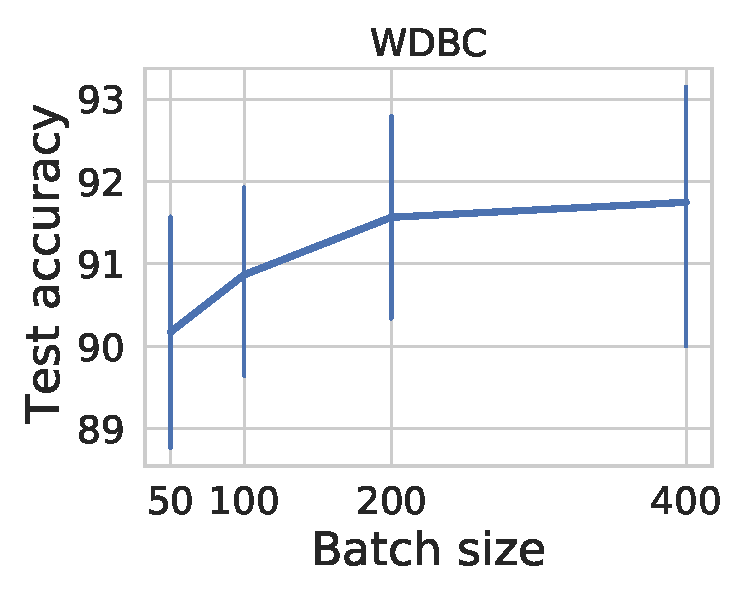
\includegraphics[scale=0.3]{figures/interpretability/imli/batch_size_test_accuracy_wdbc}}
	\subfloat{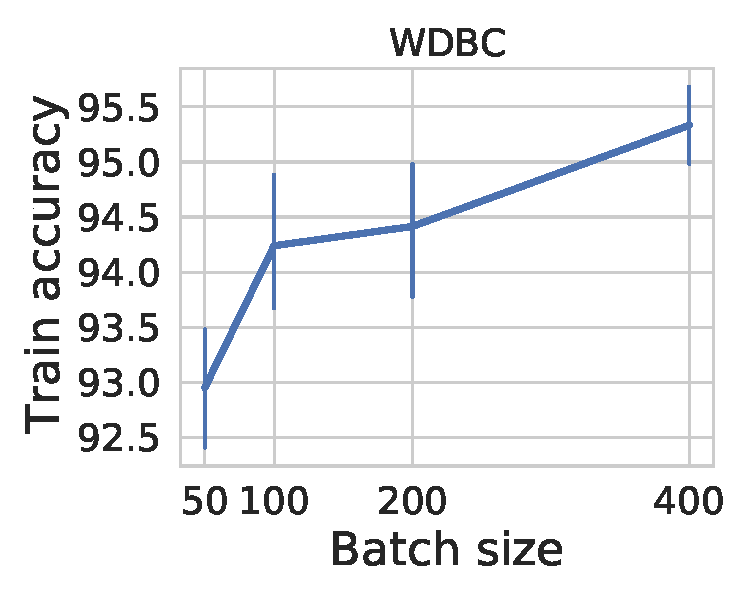
\includegraphics[scale=0.3]{figures/interpretability/imli/batch_size_train_val_accuracy_wdbc}}
	\subfloat{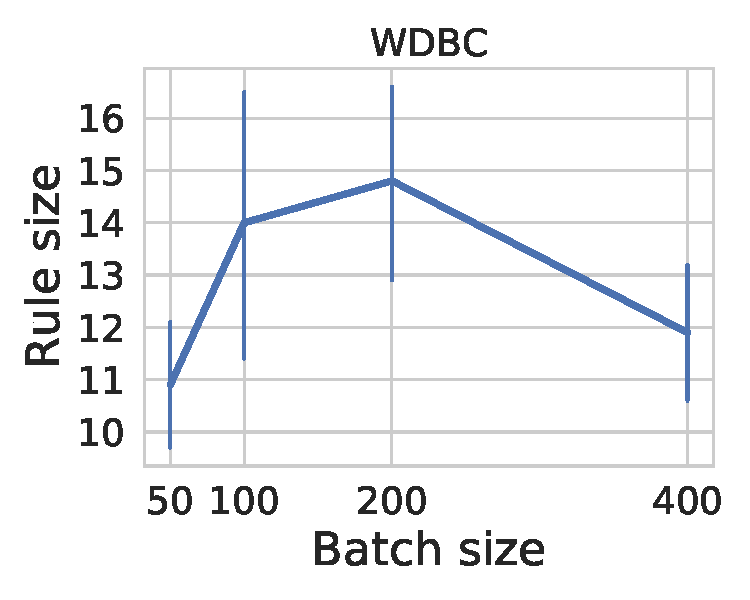
\includegraphics[scale=0.3]{figures/interpretability/imli/batch_size_predicate_count_wdbc}}
	\subfloat{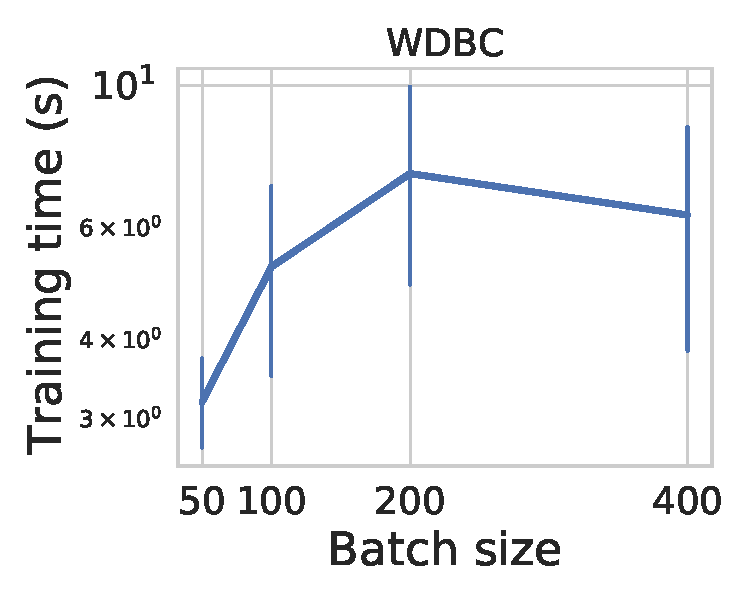
\includegraphics[scale=0.3]{figures/interpretability/imli/batch_size_train_val_fit_time_wdbc}}
	
	
	\subfloat{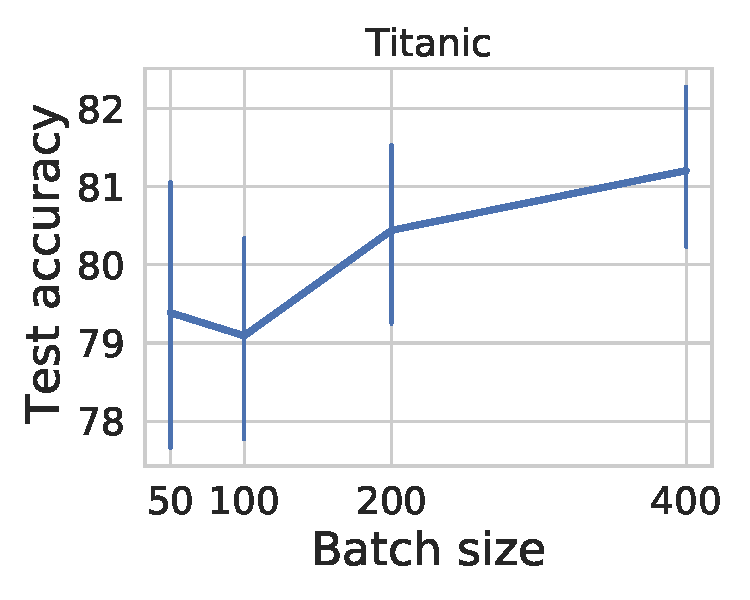
\includegraphics[scale=0.3]{figures/interpretability/imli/batch_size_test_accuracy_titanic}}
	\subfloat{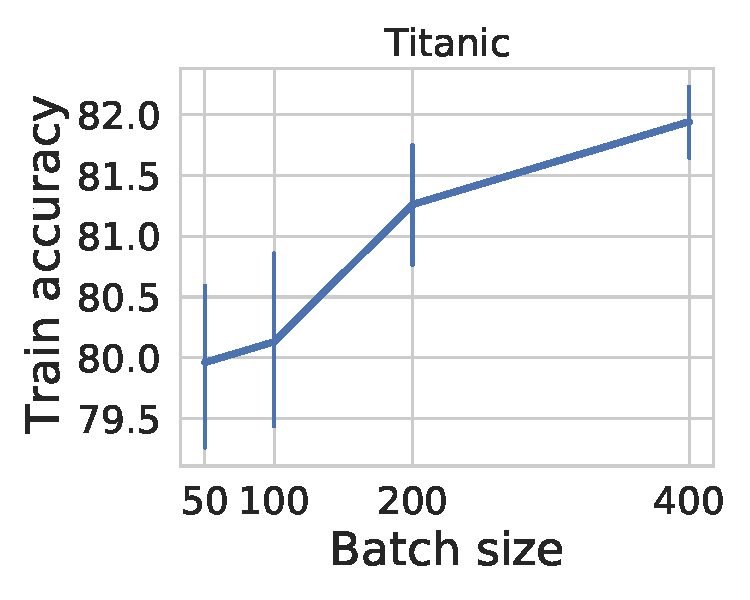
\includegraphics[scale=0.3]{figures/interpretability/imli/batch_size_train_val_accuracy_titanic}}
	\subfloat{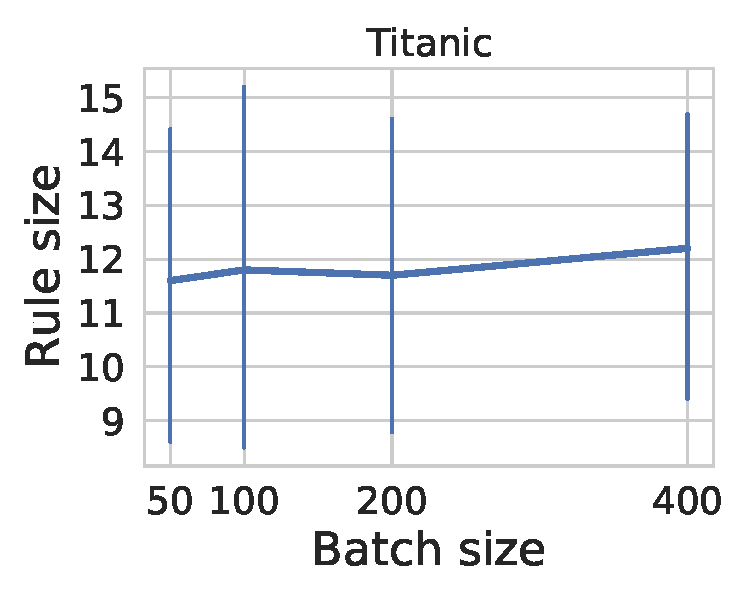
\includegraphics[scale=0.3]{figures/interpretability/imli/batch_size_predicate_count_titanic}}
	\subfloat{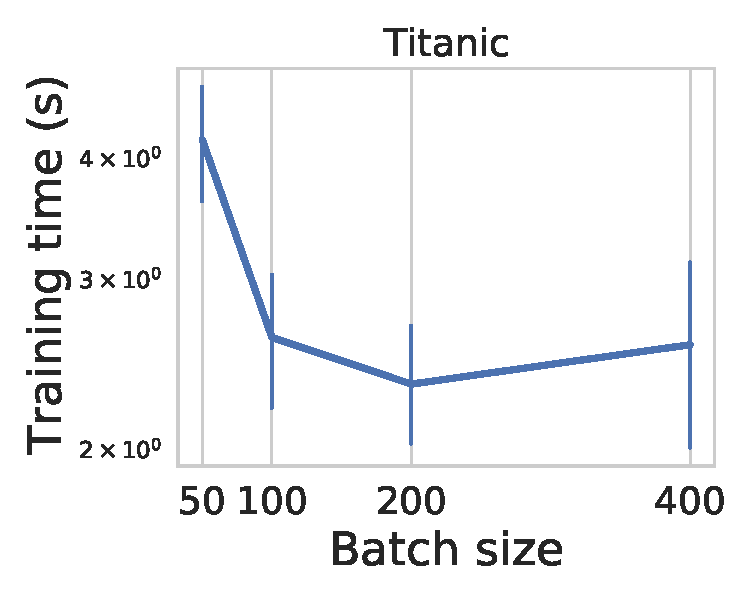
\includegraphics[scale=0.3]{figures/interpretability/imli/batch_size_train_val_fit_time_titanic}}	
	
	\subfloat{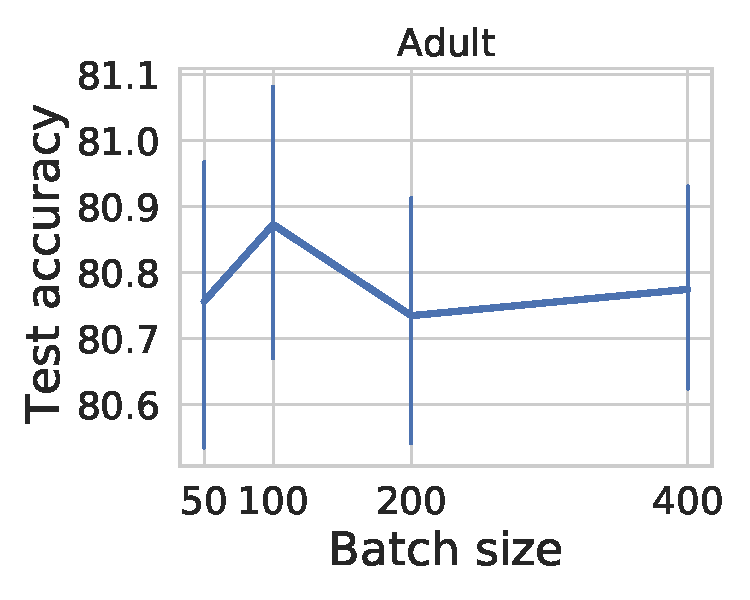
\includegraphics[scale=0.3]{figures/interpretability/imli/batch_size_test_accuracy_adult}}
	\subfloat{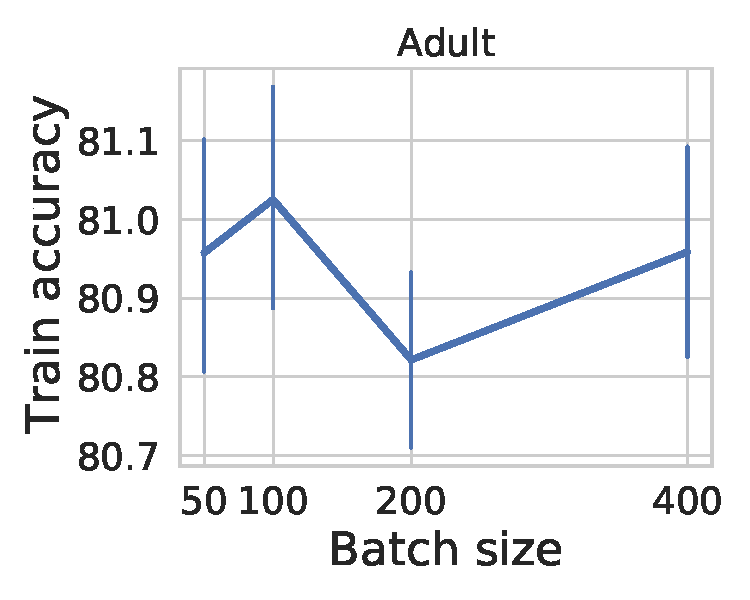
\includegraphics[scale=0.3]{figures/interpretability/imli/batch_size_train_val_accuracy_adult}}
	\subfloat{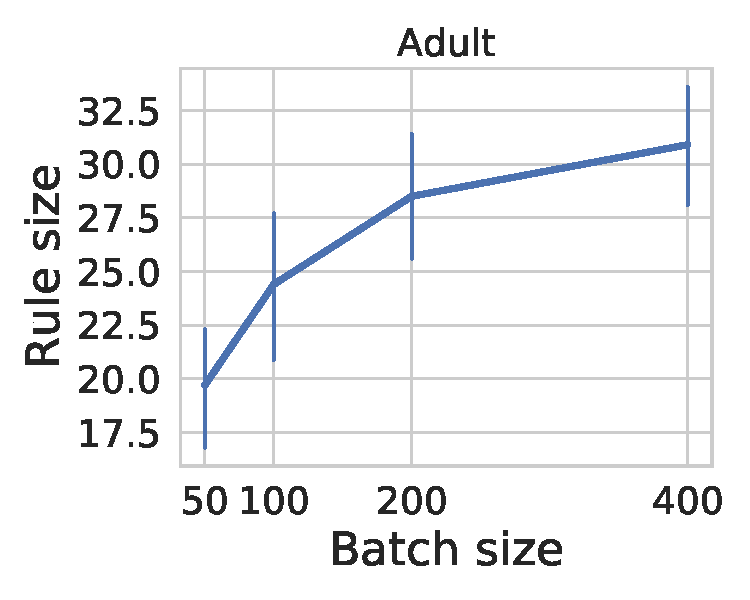
\includegraphics[scale=0.3]{figures/interpretability/imli/batch_size_predicate_count_adult}}
	\subfloat{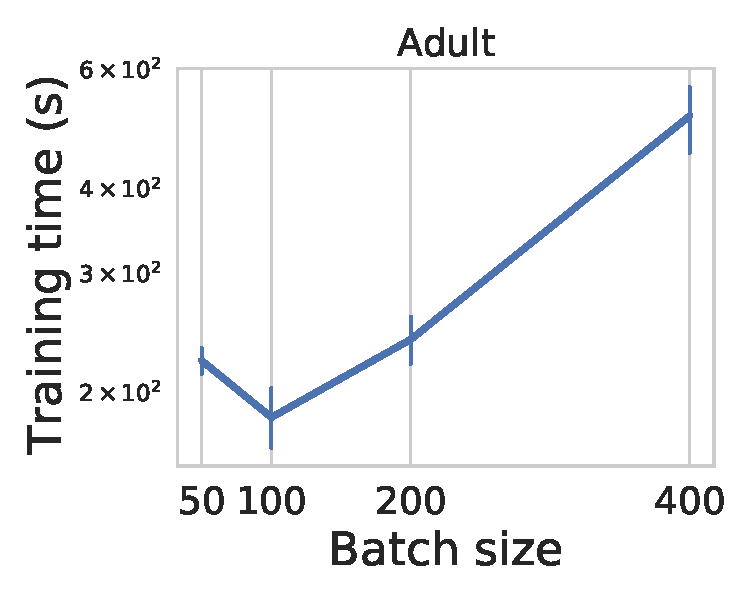
\includegraphics[scale=0.3]{figures/interpretability/imli/batch_size_train_val_fit_time_adult}}
	
	
	
	
	
	\caption[Effect of batch-size in {\imli}]{Effect of bath size on accuracy (test and train), rule-size, and training time. As we consider more samples in a mini-batch, {\imli} generates more accurate and larger size classification rules.}
	\label{interpretability_imli_fig:effect_of_batch_size}
\end{figure}




\begin{comment}


\begin{figure}
	
	
	
	\subfloat{\includegraphics[scale=0.25]{figures/interpretability/imli/dataset_parkinsons_cactus_train_val_fit_time}}
	\subfloat{\includegraphics[scale=0.25]{figures/interpretability/imli/dataset_wdbc_cactus_train_val_fit_time}}
	\subfloat{\includegraphics[scale=0.25]{figures/interpretability/imli/dataset_pima_cactus_train_val_fit_time}}
	
	\subfloat{\includegraphics[scale=0.25]{figures/interpretability/imli/dataset_titanic_cactus_train_val_fit_time}}
	\subfloat{\includegraphics[scale=0.25]{figures/interpretability/imli/dataset_magic_cactus_train_val_fit_time}}
	\subfloat{\includegraphics[scale=0.25]{figures/interpretability/imli/dataset_toms_cactus_train_val_fit_time}}
	
	\subfloat{\includegraphics[scale=0.25]{figures/interpretability/imli/dataset_credit_cactus_train_val_fit_time}}
	\subfloat{\includegraphics[scale=0.25]{figures/interpretability/imli/dataset_adult_cactus_train_val_fit_time}}
	\subfloat{\includegraphics[scale=0.25]{figures/interpretability/imli/dataset_bank_cactus_train_val_fit_time}}
	
	\subfloat{\includegraphics[scale=0.25]{figures/interpretability/imli/dataset_connect_cactus_train_val_fit_time}}
	\subfloat{\includegraphics[scale=0.25]{figures/interpretability/imli/dataset_dota_cactus_train_val_fit_time}}
	\subfloat{\includegraphics[scale=0.25]{figures/interpretability/imli/dataset_weatherAUS_cactus_train_val_fit_time}}
	
	
	\caption{Comparison among interpretable classifiers.}
	\label{interpretability_imli_fig:interpretable_classifiers_all}
\end{figure}


%
%\begin{figure}
%	\subfloat{\includegraphics[scale=0.25]{figures/interpretability/imli/all_datasets_cactus_predicate_count}}
%	\subfloat{\includegraphics[scale=0.25]{figures/interpretability/imli/all_datasets_cactus_test_accuracy}}
%	\subfloat{\includegraphics[scale=0.25]{figures/interpretability/imli/all_datasets_cactus_train_val_fit_time}}
%	\caption{}
%\end{figure}



\end{comment}


%











				
\section{Chapter Summary}
\label{interpretability_imli_sec:conclusion}
Interpretable machine learning is gaining more focus with applications in many safety-critical domains. Considering the growing demand for interpretable models, it is challenging to design learning frameworks that satisfy all aspects: being accurate, interpretable, and scalable in practical classification tasks.  In this paper, we have proposed a MaxSAT-based framework {\imli} for learning interpretable rule-based classifiers expressible in CNF formulas. {\imli} is built on efficient integration of incremental learning, specifically mini-batch and iterative learning, with MaxSAT-based formulation.  In our empirical evaluation, {\imli} achieves the best balance among prediction accuracy, interpretability, and scalability. In particular, {\imli} demonstrates competitive prediction accuracy and rule-size compared to existing interpretable rule-based classifiers. In addition, {\imli} achieves impressive scalability than both interpretable and non-interpretable classifiers by learning interpretable rules on million-size datasets with higher accuracy.  Finally, {\imli}  generates other popular interpretable classifiers such as decision lists and decision sets using the same framework.


%\section*{Acknowledgments}
%This work was supported in part by National Research Foundation, Singapore under its NRF Fellowship Programme [NRF-NRFFAI1-2019-0004 ] and AI Singapore Programme [AISG-RP-2018-005],  and NUS ODPRT Grant [R-252-000-685-13]. The computational work for this article was performed on resources of Max Planck Institute for Software Systems, Germany and the National Supercomputing Centre, Singapore (\url{https://www.nscc.sg}.
%%
%%
%%
%%		Relaxed CNF
			\chapter{Classification Rules in Relaxed Logical Form}
%				\section{abstract}
	 Machine learning algorithms that produce  rule-based predictions   in Conjunctive Normal form (CNF) or in Disjunctive Normal form (DNF) are arguably some of the most interpretable ones. For example, decision set is an interpretable model in practice, that represents the decision function in the form of DNF. In this paper, we consider relaxed definitions of standard OR/AND operators which allow exceptions in the construction of a clause and also in the selection of clauses in a rule. Building on these relaxed definition,  we introduce \textit{relaxed-}CNF rules, which are motivated by the popular usage of checklists in the medical domain and generalizes the widely employed rule representations including CNF, DNF, and decision sets.  While the combinatorial structure of relaxed-CNF rules offers exponential succinctness, the naive learning techniques are computationally expensive. 	 To this end, we  propose a novel incremental mini-batch learning procedure, called {\crr}, that employs  advances in the  Mixed-Integer Linear Programming (MILP) solvers to efficiently learn relaxed-CNF rules.  
	 Our  experimental analysis demonstrates that {\crr} can generate relaxed-CNF rules, which are more accurate and sparser compared to the alternative rule-based models. 


				%%\vspace{-5pt}
%\section{Introduction}
%%\vspace{-5pt}
%\label{interpretability_crr_sec:introduction}


The widespread adoption of prediction systems in various safety-critical domains such as medical diagnosis, law, education, and many others has led to the increased importance of presenting the decision functions in interpretable representations~\cite{K2001,MVBB2005,SAD2015,S2014,TV2013}.  To enable  safe, robust, and trustworthy integration of such systems, the end users require them to support interpretability, privacy, and fairness in decision-making~\cite{DF2018,VML2012,WRLKM2015,ZUR2017}. In this context,  rule-based representations are considered interpretable in presenting the decision functions to users~\cite{LKCL2019,MM18,WR2015,WRDLKM2017}. A recent body of work has studied sparsity-inducing objectives for classification rules in CNF ({Conjunctive Normal Form}) or DNF ({Disjunctive Normal Form}) and demonstrated that they often achieve high interpretability\textemdash defined in terms of rule-sparsity\textemdash with a minimal sacrifice in classification accuracy ~\cite{ghosh19incremental,LKCL2019,MM18}. Although CNF/DNF rules are considered interpretable, they are less expressive compared to Boolean cardinality constraints in propositional logic. A Boolean cardinality constraint allows one to express numerical bounds on Boolean variables~\cite{sinz2005towards}. In this work, we introduce a novel formulation of interpretable classification rules, namely \emph{relaxed-CNF}, which achieve benefits of  both worlds: it is interpretable similar to CNF/DNF  but more expressible by allowing cardinality constraints in the representation.


We find the motivation of relaxed-CNF rules from checklists. A checklist is a list of conditions that one needs to check, e.g., a list of items to take on a travel trip.  Checklists have several applications in interpretable decision making~\cite{M1976,gage2001validation}, particularly in the medical domain. For example, the  CHADS2 score in medicine is a clinical prediction rule for estimating the risk of stroke~\cite{gage2001validation}. Another example of checklists is a psychometric test, known as Myers–Briggs Type Indicator (MBTI)~\cite{M1976}, which indicates differing psychological preferences in how people perceive the world around them and make decisions.  An influential study on the importance of {checklists}~\cite{G2010} finds that highly complex and specialized problems can be handled smoothly by the development and consistent usage of checklists, which we formally call as relaxed-CNF rules. 


We now provide an introduction to relaxed-CNF rules. In interpretable rule-based classification, the simplest logical rules are single level-rules: ORs or ANDs of Boolean \textit{literals}, where each literal denotes either a Boolean input feature or its negation. A \emph{clause} is a collection of $ N $ literals connected by  OR/AND. To satisfy a clause, an OR operator requires $ 1 $ out of $ N $ literals to be assigned to  $ 1 $ in the clause, while an AND operator requires all $N$ out of $N$ literals to be assigned to  $ 1 $. A CNF   formula  is a conjunction (AND) of {clauses} where each clause is a disjunction (OR) of {literals}, and  a DNF  formula is a disjunction of clauses where each clause is a conjunction of literals. Therefore, CNF  and DNF  formulas can be viewed as two-level rules with several applications in interpretable decision-making. For example, a decision set is a DNF rule referring to a set of ``if-else'' conditions~\cite{ignatiev2018sat,lakkaraju2016interpretable}.  In this chapter, we consider a richer set of logical formulas that capture the structure of checklists. To this end, we consider \emph{hard}-OR clauses, where at least $ M > 1$ out of $ N $ literals are assigned to $ 1 $, and we similarly define {\emph{soft}-AND} clauses which allow some of the literals (at most $ N-M $) to be $ 0 $. To be precise,  the definitions of hard-OR and soft-AND overlap. Consequently, we use hard-OR when $M \le N/2$ and soft-AND otherwise. To extend the standard definition of CNF (which is ANDs of ORs),  we define \emph{relaxed}-CNF to denote soft-ANDs of hard-ORs. Similarly, \emph{relaxed}-DNF is hard-ORs of soft-ANDs. Since   hard-OR and soft-AND are differentiated based on the value of $ M $ and $ N $, relaxed-CNF and relaxed-DNF have the same structural representation. In early work, Craven and Shavlik~\cite{craven1996extracting} considered single level $ M $-of-$ N $ rules to explain black-box neural-network classifiers. Recently, Emad et al.~\cite{EVM2015} have developed a semi-quantitative group testing approach for learning sparse single level $M$-of-$N$ rules, which are quite restrictive in their ability to fit the data. In contrast, in this work, we study a much richer family of two-level relaxed-CNF rules. 





\begin{figure*}
	\begin{center}
		\includegraphics[scale=.65]{figures/interpretability/relaxed-cnf/checklist.pdf}
	\end{center}
	\caption[Illustration of a relaxed-CNF classification rule]{An illustrative example of a  relaxed CNF classification rule, which describes the decision function in the form of a  two-level checklist. This classifier is learned on the WDBC (Wisconsin diagnostic breast cancer) dataset and it predicts whether a tumor cell is malignant or not based on the characteristics of the  tumor cell. The first column in each checklist contains Boolean literals. An entry in the second column is  $ 1 $ if the corresponding literal is true by an observed tumor cell, and $ 0 $ otherwise. In the first level, checklist A (resp.\ B) is true if the count of true  predicates is at least $ 2 $ (resp.\ $ 3 $). In the second level, a tumor cell is predicted as malignant if the count of true checklists is at least $ 1 $. }
	\label{interpretability_crr_exmpl:wdbc}
\end{figure*}




 {Relaxed-CNF rules are  more flexible than pure CNF rules, and they can accurately fit more complex classification boundaries.} For example, relaxed-CNF clauses  allow  a compact encoding of the majority function\footnote{The majority function is a Boolean function that evaluates to $ 0 $ when half or more arguments are false, and $ 1 $ otherwise (\url{https://en.wikipedia.org/wiki/Majority_function}).} in Boolean logic, which would require exponentially many clauses in CNF, showing the exponential gap in the succinctness of the two representations.  In addition, relaxed-CNF and CNF rules have the same functional form where a user has to compute the sum of true literals/clauses  and then compare the sum  to  different thresholds {(as in the example in Figure~\ref{interpretability_crr_exmpl:wdbc})}. From the computational perspective, the structural flexibility of relaxed-CNF compared to CNF/DNF makes it harder to learn. Therefore, in this chapter, we ask the following research question: \textit{can we design a combinatorial framework to efficiently learn relaxed-CNF rules?}

The primary contribution of this chapter is an affirmative answer to the above question by proposing an efficient combinatorial learning framework for relaxed-CNF rules, namely {\crr} (\textbf{C}lassification \textbf{R}ules in \textbf{R}elaxed form). In CRR, we construct a learning objective to maximize both the prediction accuracy and the rule-sparsity of the generated classification rule. To this end, we design a  Mixed-Integer Linear Programming (MILP) formulation for learning the optimal relaxed-CNF rule from data. To learn a $ k $-clause relaxed-CNF rule (say $ \Rule $) using the na\"ive MILP formulation, the size of the MILP query expressed as the number of constraints is $ \mathcal{O}(nk) $, where $ n $ is the number of training samples in the dataset. Consequently, this formulation fails to handle large datasets. To address the scalability of {\crr},  we propose an efficient mini-batch training methodology, where we incrementally learn $ \Rule $ from data by iteratively solving smaller MILP queries corresponding to batches. 

{Through a comprehensive experimental evaluation over datasets from the UCI and Kaggle repository, we observe that {\crr} with relaxed-CNF rules achieves an improved trade-off between accuracy and rule sparsity and scales to datasets with more than $ 10^5 $ samples. More significantly, {\crr} generates relaxed-CNF rules with higher accuracy than CNF rules generated by~\cite{ghosh19incremental}. Furthermore, compared to decision lists generated by~\cite{C1995}, relaxed-CNF rules are sparser in large datasets.}
%can also reach the same level of accuracy compared to plain CNF/DNF rules with smaller relaxed-CNF rules. 
%
%We have conducted a comprehensive experimental study on the datasets from the UCI repository. Our empirical study demonstrates  an increase in the prediction accuracy for choosing relaxed-CNF rules over regular CNF rules. The incremental approach achieves runtime scalability without loss of accuracy. 


\begin{comment}
\begin{example}
	\label{interpretability_crr_exmpl:wdbc}
	As an example, we illustrate a relaxed-CNF rule learned 
	for  Breast Cancer Wisconsin Diagnostic Dataset (WDBC) from UCI repository. 
	The dataset is used to predict whether the tumor is  malignant or benign based on the characteristics of  a tumor cell. We can learn the following rule for detecting malignant cancer. 
	%
	
	
	%\vspace{-13pt}
	\[
	\boxed{
		\begin{split}
		&\text{Tumor is diagnosed as malignant if, }\\
		&[ \{  (\text{ smoothness }\ge 0.089)   + (\text{standard error of area  }\ge 53.78)  + \\ & (\text{largest radius }\ge  18.225)   \}\ge 2  ] \; + \\&  [   \{(98.76\le \text{ perimeter } < 114.8)  +    (\text{largest smoothness }\ge  0.136) \\& 
		+ (105.95 \le \text{ largest perimeter }  < 117.45)    \}\ge 2  ]  \ge 1 \end{split}}
	\]
	
	
	
	
	The generated rule has two clauses presented within the square brackets. Each clause consists of three literals  (presented within the parentheses) and a comparator with a \textit{threshold  on literals} (shown outside the curly brace). For example, ``smoothness $ \ge  0.089  $'' is a literal/predicate and is assigned $ 1 $ (or true)  if a tumor cell satisfies this characteristic and $ 0 $ otherwise. Inside a clause, 
	we connect the literals  using ``$ + $'' to sum   the number of true  literals  and then compare the sum with the threshold, which is $ 2 $ in both clauses in the above example. A clause is assigned $ 1 $ (or true)  if the sum of true literals satisfies the threshold.
	Similarly, each clause is connected using ``$ + $'' to sum the number of true clauses in the rule. Finally, the rule is satisfied, i.e, a tumor is diagnosed as malignant, if the number of true clauses is at least equal to the \textit{threshold on clauses}, which is  $ 1 $ in this example. In this context, we choose to measure the size of the rule by the number of literals it contains, which in this case is   $ 3+3=6 $.   In this  example, the decision function is represented  as a two-level checklist, where one would  check items (i.e., literals/predicates) inside a checklist in the first level   and then check among the checklists (i.e., clauses) in the second level. 
\end{example}

\end{comment}




%KSM: Please feel free to comment out the text below if it exceeds page limit
The rest of the chapter is organized as follows. We discuss related works in Section~\ref{interpretability_crr_sec:related_work}, introduce the notation and preliminaries in Section~\ref{interpretability_crr_sec:preliminaries} and formulate the problem in Section~\ref{interpretability_crr_sec:problem}. We describe the main contribution of this chapter, $ \crr $,  in Section~\ref{interpretability_crr_sec:ilp} and extend to an incremental mini-batch learning in Section~\ref{interpretability_crr_sec:inc_ilp}. We then describe the experimental results in Section ~\ref{interpretability_crr_sec:experiment} and conclude in Section~\ref{interpretability_crr_sec:conclusion}. 








%				\section{Related Work}
\label{interpretability_crr_sec:related_work}
In the growing field of interpretable machine learning,  several rule-based systems such as decision trees~\cite{narodytska2018learning},  decision lists~\cite{R1987}, decision sets~\cite{ignatiev2018sat,lakkaraju2016interpretable} and classification rules~\cite{C1995,DGW2018} have been proposed over the years. More recently, a Bayesian framework has been adopted to learn rule sets~\cite{WRDLKM2017}, rule lists \cite{LRMM2015},  and falling rule lists~\cite{WR2015}. Building on the connection between rule learning and Boolean compression sensing,  a rule-based classification system was proposed to trade-off classification accuracy and representation size~\cite{MV2013}. Su et al.~\cite{SWVM2015} proposed an extension that allows two-level Boolean rules. In addition to designing classifiers that produce forms amenable to end-users, there is a large body of work to describe the working of opaque models (model-agnostic interpretability)~\cite{LKCL2019,lundberg2017unified,ribeiro2016should}.  While our work can also be applied to interpret black-box classifiers, we do not pursue this direction in this paper and leave for future work. 


In recent work,  Ghosh and Meel~\cite{ghosh19incremental} propose an incremental approach for efficiently learning CNF classification rules using a MaxSAT-based framework. They adopt a sequential partition-based training methodology in incremental learning. Although the said approach achieves the runtime improvement,  the generated rules highly depend on the order/position of samples in the training dataset. In contrast, the incremental framework proposed in this work does not suffer from strong dependencies on the order of samples in the training dataset.


%				%\vspace{-8pt}
\section{Preliminaries}
\label{interpretability_crr_sec:preliminaries}
We use capital  boldface letters such as $\mathbf{X}$ to denote matrices, while lower boldface letters $\mathbf{y}$ are reserved for vectors. For a matrix $\mathbf{X}$, $\mathbf{X}_i$  represents the $ i $-th row of $\mathbf{X}$ while for a vector $\mathbf{y}$, $y_i$ represents the $ i $-th element of $\mathbf{y}$. 
% For a vector/set $ \mathbf{u} $ we  use $ |\mathbf{u}| $ to denote the number of elements in $ \mathbf{u} $.

% introduce cardinality constraint in this part

Let $F$ be a Boolean formula and  $\mathbf{b} = \{b_1,b_2,\dots ,b_m \}$ be the set of Boolean propositional variables appearing in $F$. A literal $ v_i $ is a variable ($b_i$) or its complement ($\neg b_i$).  A \emph{satisfying assignment} or a \emph{witness} $ \sigma $ of $F$ is an assignment of variables in $\mathbf{b}$ that makes $F$ evaluate to $ 1 $ and is denoted as $ \sigma \models F $.  If $\sigma$ is an assignment of variables and $b_i \in \mathbf{b}$, we use $\sigma(b_i)$ to denote the value assigned to $b_i$ in $\sigma$. $F$ is in CNF if $F :=  \bigwedge_{i=1}^k C_i$ is conjunction (AND) of clauses, where each clause $C_i :=  \bigvee_j v_j $  is represented as a disjunction (OR) of literals.  {A hard OR (resp. soft AND) clause $ (C,\eta) $ has an extra parameter $ \eta $, where $ \eta $ is the threshold on the literals in $ C $.} Let $ \mathbb{1}[true]=1 $ and $ \mathbb{1}[false]=0 $. Motivated by checklists, we propose relaxed-CNF where in addition to $F$, we have two more parameters $\eta_c$ and $\eta_l$. We say that $(F,\eta_c, \eta_l)$ is in relaxed-CNF and $ \sigma $ is its witness if $\sigma \models (F,\eta_c, \eta_l)$ whenever $\sum_{i=1}^k \mathbb{1}[\sigma \models (C_i,\eta_l)] \ge \eta_c$ where $\sigma \models (C_i, \eta_l)$ iff $\sum_{v \in C_i} \mathbb{1}[\sigma \models v] \geq \eta_l$. Informally,  $\sigma$ satisfies a clause $(C_i, \eta_l)$ if  at least $\eta_l$ literals in $C_i$ are set to true by $\sigma$ and $\sigma$ satisfies $(F,\eta_c, \eta_l)$ if at least $\eta_c$ of $\{(C_i,\eta_l)\}$ are true. In the  example in Figure~\ref{interpretability_crr_exmpl:wdbc}, $ \eta_c=1 $ and $ \eta_l=2 $. 


\begin{theorem}[\cite{benhamou1994two}]
	\label{interpretability_crr_thm:succinctness}	
	Let $ (C,\eta) $ be a clause in relaxed-CNF where  $ C $ has $ m  $ literals and $ \eta \in \{1,\dots,m\} $ is the threshold on literals.  An equivalent compact encoding of $ (C,\eta) $  into a CNF formula $ F= \bigwedge_i C_i $ requires $ {m \choose{m-\eta+1}} $  clauses where each clause is distinct and has $ m-\eta+1 $ literals of $ (C,\eta) $. Therefore,  the total number of literals in $ F $ is $ (m-\eta+1){m\choose{m-\eta+1}} = m $ when $ \eta=1 $, otherwise $ (m-\eta+1){m\choose{m-\eta+1}} > m $.
\end{theorem}


%\red{Relaxed-CNF rules generalize both CNF and DNF rules. }
%Properly define k-DNF, i.e., every clause has k literals. Every $-$DNF rule can be viewed as a relaxed-CNF rule with $\eta_c = 1$ and $\eta_l = k$. Similarly, every $k-$CNF rule can be viewed as a relaxed-CNF rule with $\eta_c=k$ 
% $ F $ is a relaxed-CNF if $ F:=[\sum_{i=1}^k C_i] \ge \eta_c $, where each clause $ C_i := [\sum_j l_j] \ge \eta_l $. Here $ \eta_c $  and $ \eta_l $ are two positive integer thresholds.


%We use $|C_i|$ to denote the number of literals in $C_i$.  
%A \emph{pseudo-boolean constraint} over literals is defined as $ \sum_i a_i\cdot l_i \ge \card; a_i,\card \in \mathbb{R} $.  The special case $ \sum_i l_i \ge \card $ is denoted as a \emph{cardinality constraint}. In the  case of cardinality constraint, $ \card $ is called a  cardinality constant and $ \card \in \mathbb{Z} ^+$. 
%A pseudo-boolean constraint can be encoded into a CNF formula by applying the state of the art encoding technique. 
%Therefore, a cardinality constraint is a variant of general  CNF clause. 
% Specifically,  a cardinality constraint is satisfied if at least $ \card $ literals in that clause are assigned to $ 1 $, which is different from a CNF clause where $ \card=1 $ is applied.


Between two vectors  $\mathbf{u}$ and $\mathbf{v}$ of the same size over Boolean variables/constants (e.g.,  $ 0 $, $ 1 $), we use $\mathbf{u} \circ \mathbf{v} $  to denote the inner product, i.e.,     $\mathbf{u} \circ \mathbf{v} = \sum_{i} (u_{i} \cdot v_{i})$, where $u_{i}$ and $v_{i}$ are a variable/constant  at the $i$-th index of $\mathbf{u}$ and $\mathbf{v}$, respectively. In this context,  the operator ``$\cdot$'' between a variable and a constant follows the standard interpretation, i.e., $0 \cdot b = 0$ and $1 \cdot b = b$. 

%KSM: Define CNF and define relaxed-CNF before you start talking about clauses of CNF/relaxed-CNF. Also, define literal

We consider a standard binary classification problem, where we are given a collection of 
training samples $\{ (\mathbf{X}_i, y_i) \}$. For sample $ i $, $\mathbf{X}_i \in \{0,1\}^m$ contains the valuation of the feature vector $\mathbf{x} = \{x_1, x_2, \dots, x_m\}$, and $y_i \in \{0,1\}$ is the binary class label.
A classifier {\Rule} is a mapping that takes in the feature vector $\mathbf{x}$ and returns a class $\hat{y} \in \{0,1\}$, i.e., $\hat{y} = \Rule(\mathbf{x})$. The goal is not 
only to design $\Rule$ to approximate the training set, but also to generalize to unseen samples arising from the same distribution. 
We focus on classifiers that can be expressed  as  relaxed-CNF. We use $\clause(\Rule,i)$ to denote  the  $i$-th clause of $\Rule$ and $ |\clause(\Rule,i)| $ to  denote the size of  $\clause(\Rule,i)$, which is measured as the number of literals in the $ i $-th clause. Furthermore, we use $|\Rule|$ to denote the rule-size of classifier $ \Rule $, which is defined as the number of literals in all the clauses, i.e., $|\Rule| = \Sigma_i |\clause(\Rule,i)|$. In the example in Figure~\ref{interpretability_crr_exmpl:wdbc}, $ |\Rule| = |\clause(\Rule, 1)| + |\clause(\Rule, 2)| = 3+3=6 $.


In this work, we consider the learning problem as an optimization problem, wherein we reduce the construction of $\Rule$ to computing assignments of appropriately designed variables.  An optimization problem consisting of Boolean variables can be solved using Integer Linear Programming (ILP) where each variable takes value either $ 0 $ or $ 1 $.\footnote{The problem can be viewed as either ILP or MaxSAT, but we obtained better performance from ILP solvers.} Given an objective function and a set of constraints comprising of variables with range $ \{0,1\} $, ILP finds an optimal assignment of variables that minimizes the objective function.
% We assume $ \sigma(\cdot) $ is a function over variables which outputs the assignment (either $ 0 $ or $ 1 $) of each variable and the task is to learn $ \sigma $ by solving an ILP query.  
% The inner knowledge of how ILP solves the problem, is not required to understand the paper. 

%In our context, we define $ \Rule $ to be a set of important features which we aim to identify and $ \Rule \subseteq \mathbf{x} $. We use the notation $ |\Rule| $ to denote the count of features in $ \Rule $.For example, let $ \mathbf{x}=\{x_1,x_2,x_3,x_4\} $ and we learn  $ \Rule=\{x_1,x_3,x_4\} $. Therefore $ |\Rule|=3 $. 



%We define two rules  $ \Rule_1 $ and $ \Rule_2 $ to be  equivalent  if $ \forall i,\Rule_1(\X_i)=\Rule_2(\X_i) $. 




%We denote the set of all witnesses of $F$ by {\satisfying{F}}.



%In this work, we focus on the weighted variant of CNF wherein a weight function is defined over clauses. For a clause $C_i$ and weight function {\weight{\cdot}}, we use {\weight{C_i}} to denote the weight of clause $C_i$. We say that a clause $C_i$ is hard if $\weight{C_i} = \infty$, otherwise $C_i$ is called a soft clause.  To avoid notational clutter, we overload {\weight{\cdot}} to denote the weight of an assignment or clause, depending on the context. We define weight of an assignment $\sigma$ as the sum of weight of clauses that $\sigma$ does not satisfy. Formally, $\weight{\sigma} = \Sigma_{i | \sigma \not\models C_i} \weight{C_i}$.

%Given $F$ and weight function $\weight{\cdot}$, the problem of {MaxSAT} is to find an assignment $\sigma^*$ that has the minimum weight, i.e.  $\sigma^* = \MaxSAT(F,W)$ if $\forall \sigma \neq \sigma^*, \weight{\sigma*} \leq \weight{\sigma}$. Our formulation will have positive clause weights, hence MaxSAT corresponds to satisfying as many clauses as possible, and picking the strongest clauses among the unsatisfied ones. 
%Note that the above formulation is different from the typical definition of {\MaxSAT} but the difference is only syntactic. Borrowing terminology of community focused on developing {MaxSAT} solvers, we are solving a partial weighted {MaxSAT} instance wherein we mark all the clauses with $\infty$ weight as hard and clauses with other positive value less than $ \infty $ weight as soft  and ask for a solution that optimizes the partial weighted {MaxSAT} formula.  The knowledge of encoding a  cardinality constraint into CNF clauses, the  inner working of {MaxSAT} solvers,  and  the encoding of our representation into weighted {MaxSAT} is not required for this paper.   



				%\vspace{-2pt}
\section{Problem Formulation}
\label{interpretability_crr_sec:problem}
We now present the formal definition of the problem. Given  (i) an instance space   $ (\mathbf{X}, \mathbf{y})$, where $ \mathbf{X} \in \{0,1\}^{n\times m} $ is the feature matrix with $ m $ binary features and $ n $ samples,\footnote{$\mathbf{X}$ contains both the features and their complements as columns as in~\cite{MV2013}.} and $ \mathbf{y} \in \{0,1\}^n $ is the class label vector, (ii) {a positive integer $ \noclause $ indicating the number of clauses in the desired rule}, (iii)  an integer threshold on literals $ \card_{l} \in  \{0,\dots,m\} $ indicating  the  minimum number of literals required to be true  to satisfy a clause, (iv)  an  integer threshold on clauses $ \card_{c} \in  \{0,\dots,k\} $ indicating the minimum number of clauses required to be  true  to satisfy a formula, and  (v) the data-fidelity  parameter $ \lambda \in [0,1]$, we  learn  a classification rule $ \Rule $, that is expressed as a $ k $ clause relaxed-CNF formula. 

% \[\hat{y}=\Rule(\mathbf{x})=I[\sum_{x_i\in\Rule, \Rule \subseteq \mathbf{x} } x_i \ge k]\]

Our goal is to find rules that balance two 
goals:   being accurate while also sparse to avoid over-fitting.  
To this end, we seek to minimize the total number of literals in all clauses, which motivates us to  find $ \Rule  $ with minimum  $ |\Rule| $. In particular, suppose $ \Rule $ classifies all samples correctly, i.e., $ \forall i, y_i=\Rule(\mathbf{X}_i) $. Among all the rules that classify all samples correctly,  we choose the sparsest  such $ \Rule $: 


%\vspace{-10pt}
\[
\min\limits_{\mathcal{R}} |\mathcal{R}|\text{ such that }\forall i, y_i=\mathcal{R}(\mathbf{X}_i)
\]
%\vspace{-10pt}

% $ |\mathcal{R}|=\sum_{i=1}^k |C_i (\Rule)| $ is the  total number of literals appearing in $ \mathcal{R} $. 


In practical classification tasks, perfect classification is very unusual. Hence, we need to balance rule-sparsity with prediction error.  Let $ \mathcal{E}_\mathcal{R} $   be  the set of samples which are misclassified  by $ \mathcal{R} $, i.e., $\mathcal{E}_\mathcal{R}=\{\mathbf{X}_i | y_i \ne \mathcal{R}(\mathbf{X}_i) \}$. Hence we aim to find $ \mathcal{R} $ as follows:\footnote{In our formulation, it is  straightforward to add class-conditional weights  (e.g. to penalize  false-alarms more than mis-detects), and to allow instance weights (per sample).}

%\vspace{-12pt}
\[
\min\limits_{\mathcal{R}} \;  \frac{\lambda}{n}|\mathcal{E}_\mathcal{R}| + \frac{1-\lambda}{k\cdot m} |\mathcal{R}|  \text{ such that }\forall \mathbf{X}_i \in \mathcal{E}_\mathcal{R} ,y_i \ne \mathcal{R}(\mathbf{X}_i) .
\]
%\vspace{-13pt}

Each term in the  objective function is normalized in $ [0,1] $. 
The data-fidelity parameter $ \lambda \in [0,1] $  serves to balance
the trade-off between prediction accuracy and sparsity. Higher 
values of $ \lambda $ produce lower prediction errors by sacrificing the sparsity 
of $ \Rule $, and vice versa. It can be viewed as an inverse of the regularization 
parameter. 
				\section{Classification Rules in Relaxed Logical Form}
\label{interpretability_crr_sec:ilp}
In this section, we describe the main contribution of our work, {\crr}, a  framework for learning   relaxed-CNF rules.  {\crr}  converts the learning problem into  an ILP-based formulation,  learns the optimal assignment of variables and constructs rule $ \Rule $ based on the assignment. We organize the rest of this section as follows.
We  discuss the decision variables in Section ~\ref{interpretability_crr_sec:variables},  the constraints and the linear programming relaxation in Section~\ref{interpretability_crr_sec:ilp_query}, the incremental learning in Section~\ref{interpretability_crr_sec:inc_ilp}, feature discretization in Section~\ref{interpretability_crr_sec:discretization}, and adaptation of {\crr} for learning other classification rules in Section~\ref{interpretability_crr_sec:other_rules}.
% We conclude this section by describing how {\crr} can be adjusted to learn interpretable rules in other logical forms in Section~\ref{interpretability_crr_sec:other_format}.

%Given an instance space $ \{ \mathbf{X}, \mathbf{y} \} $ and  model parameters $ \noclause,\card_c,\card_l$, and  $\lambda $, {{\crr}} constructs an ILP query $ Q $  and invokes an off the shelf ILP solver to compute the underlying rule $ \Rule $.



\subsection{Description of Variables}
\label{interpretability_crr_sec:variables}
{\crr} considers two types of  \emph{decision} variables: (i) feature variables and (ii) noise or classification error variables.
Since  feature $ X_j $ can be present or not present  in each of  the  $ \noclause $ clauses, {\crr} considers $ \noclause $   variables, each denoted by $ \bool^i_j  $  corresponding to   feature $ X_j $  to denote its participation  in the $ i^\text{th} $ clause, i.e, $ \bool^i_j=\mathds{1}[j^\text{th}\text{ feature is selected in }i^\text{th}\text{ clause}]  $.  The $ q^\text{th} $ sample in the training dataset, however, can be misclassified by $ \Rule $.  Therefore, {\crr}  introduces  a noise variable $ \noise_q \in \{0,1\}  $  corresponding to the $ q^\text{th} $ sample, so that the assignment of $ \noise_q  $ can be interpreted whether $ (\mathbf{x}^{(q)}, y^{(q)}) $ is misclassified by $ \Rule $ or not, i.e., $ \noise_q=\mathds{1}[q^\text{th}\text{ sample is misclassified}] $.  Hence, the key idea of {{\crr}} for learning $ \Rule $ is to define an ILP (Integer Linear Program) query over $k \cdot m + n$  decision variables, denoted by $\{ \bool_{1}^{1}, \bool_{2}^{1}, \dots ,\bool_{m}^{1}, \dots ,\bool_{m}^{\noclause}, \noise_1, \dots ,\noise_n\}$.   In this context, we define $\boolset_i = \{\bool^i_{j} \mid j= 1,\dots,m\}$ as a \emph{vector of   feature variables} corresponding to the $ i^\text{th} $ clause.


\subsection{Construction of the ILP Query}
\label{interpretability_crr_sec:ilp_query}
In Eq.~\eqref{interpretability_crr_eq:ilp}, we discuss the ILP query $ Q $  for learning  a $ k $-clause relaxed-CNF rule  $ \Rule $. The objective function in Eq.~\eqref{interpretability_crr_eq:ilp_obj} takes care of  both the rule-sparsity and the prediction accuracy of $ \Rule $. Since {\crr} prefers a sparser rule  with as few literals as possible, we construct the objective function by preferring  $ \bool^i_j $ to be  $ 0 $. Moreover, to encourage $ \Rule $ to predict  the training samples accurately, we penalize the number of variables $ \noise_q $ that are different from $ 0 $. In this context, we utilize  the   parameter $ \lambda $ to trade off between sparsity and accuracy.  Therefore,  the objective function of the ILP query $ Q $ is to minimize the normalized sum of all  noise variables $ \noise_q $  weighed  by the data-fidelity parameter $ \lambda $ and feature variables $ \bool^i_j $ weighed by $ 1-\lambda $.

We formulate the constraints of the ILP query $ Q $ as follows. Initially, we define the range of the decision variables and   add constraints accordingly (Eq.~\ref{interpretability_crr_eq:ilp_range} and ~\ref{interpretability_crr_eq:ilp_range_2}).  For each sample, at first, we  add constraints to mimic the behavior of hard-OR of literals in a clause, and then we add constraints to apply  soft-AND of clauses in a formula (refer to Preliminaries in Chapter~\ref{chapter:preliminaries}).

We first consider the case when  the $ q^\text{th} $  sample  has positive class label (Eq.~\ref{interpretability_crr_eq:ilp_pos}). 
$ \mathbf{x}^{(q)}\circ \boolset_i \ge \card_l $ resembles the hard-OR operation of literals in a clause.  We introduce   $ k $ \emph{auxiliary} $ \{0, 1\} $ variables $ \{\noise_{q,1}, \dots, \noise_{q,k}\} $  to check whether at least $ \card_c $ clauses are satisfied, i.e., $ \noise_{q,i}=\mathds{1}[i^\text{th}\text{ clause is dissatisfied for }q^\text{th}\text{ sample}] $, which let us impose the operation of soft-AND over clauses.    We then add a constraint to make sure that at most $ k-\eta_{c} $ clauses are allowed to be dissatisfied, otherwise the noise variable $ \noise_q $  is assigned to $ 1 $, i.e., the $ q^\text{th} $ sample is detected as aw noise.  
 



A negative labeled sample has to dissatisfy  more than $ k-\card_c $ clauses in $ \Rule $ so that the sample is predicted as $ 0 $, which is equivalent to satisfying  more than $ k-\card_c$ constraints $ \mathbf{x}^{(q)}\circ \boolset_i < \eta_l  $. As mentioned earlier, we  introduce $ \{0, 1\} $ variable $ \noise_{q,i} $ to specify if the constraint $ \mathbf{x}^{(q)}\circ \boolset_i < \eta_l  $ is dissatisfied or not and  restrict the count of dissatisfied clauses $ \sum_{i=1}^k\noise_{q,i} $ to be less than $ \card_c $. 

%In the following, we present the ILP query $ Q $.


%\vspace{-15pt}
\begin{subequations}
	\label{interpretability_crr_eq:ilp}
 \begin{align} 	
% 	\begin{split}
 	&\min   \frac{\lambda}{n} \sum_{q=1}^n \noise_q + \frac{1-\lambda}{k\cdot m}\sum_{i=1}^k\sum_{j=1}^m \bool_j^i \label{interpretability_crr_eq:ilp_obj} \\
 	&\text{such that,} \notag \\
 	&\bool_j^i \in \{0,1\},  i = 1,\dots,k,  j = 1,\dots,m \label{interpretability_crr_eq:ilp_range}\\
 	& \noise_q \in \{0,1\},q = 1,\dots,n  \label{interpretability_crr_eq:ilp_range_2}\\
 	&\text{if }  \forall q \in \{1,\dots,n\},\text{ if }  y^{(q)}=1, \label{interpretability_crr_eq:ilp_pos}\\
 	&\qquad \mathbf{x}^{(q)}\circ \boolset_i+ m\noise_{q,i} \ge \eta_{l},  i = 1,\dots,k  \label{interpretability_crr_eq:ilp_ela_l_pos}\\
 	& \qquad   k\noise_q + k-\eta_c \ge \sum_{i=1}^k \noise_{q,i} \notag \\ &\qquad \noise_{q,i} \in \{0,1\},  i = 1,\dots,k \notag\\
 	&\text{if } \forall q \in \{1,\dots,n\}, y^{(q)}=0, \label{interpretability_crr_eq:ilp_neg}\\
 	&\qquad \mathbf{x}^{(q)}\circ \boolset_i < \eta_{l} + m  \noise_{q,i},  i = 1,\dots,k \label{interpretability_crr_eq:ilp_ela_l_neg}\\
 	&\qquad  k\noise_q  + \eta_{c} > \sum_{i=1}^k\noise_{q,i} \notag\\ &\qquad \noise_{q,i} \in \{0,1\},  i = 1,\dots,k \notag
% 	\end{split}
\end{align}
\end{subequations}
%\vspace{-15pt}

In the following, we show the complexity of the ILP query in terms of the number of variables and constraints. 

\begin{proposition}
	Given a training dataset with $ n $ samples and $ m $ binary features, the ILP query $ Q $ for learning a binary classification rule in relaxed-CNF has $ k\cdot m + n $ decision variables, $ k\cdot n $ auxiliary variables, and  $ k\cdot m + n\cdot (k+3)  $ integer constraints. 
\end{proposition}

An ILP solver takes  query  $ Q $ as input and returns the optimal assignment $ \sigma^* $of the variables.
We extract relaxed-CNF rule $\Rule$ from the solution  as follows. 


\begin{construction}
	\label{interpretability_crr_cons:rule}
	Let $\sigma^* = \ILP(Q)$, then $X_j \in {\clause(\Rule,i)}$ if and only if $\sigma^*(\bool_{j}^i) = 1$.
\end{construction}

%\textbf{Hardness of the ILP problem:}The ILP query in Eq.~\ref{interpretability_crr_eq:ilp} has integer constraints, and the problem is NP-hard. We prove this by reducing the presented ILP query to learn a sparse single clause CNF rule, that is consistent with the training dataset (does not make any classification error) by specifying $ k=1, \eta_{c}=1, \eta_l=1, \text{ and } \lambda=1$ in Eq.~\ref{interpretability_crr_eq:ilp}.  In this context, Malioutov et al.~\cite{MV2013} has demonstrated that learning a sparse single clause CNF rule consistent on the training dataset  is a combinatorial problem in NP-hard by showing connections between compressed sensing and sparse signal recovery~\cite{natarajan1995sparse}. 





\textbf{Learning thresholds $ \eta_l $ and $ \eta_c $:}
Given the training dataset $ \dataset $ and data-fidelity parameter $ \lambda $, one could learn the optimum value of the thresholds $ \card_{c} $ and $ \card_l $ of the desired rule $ \Rule $  by specifying their range as constraints in the ILP query $ Q $ in Eq.~\ref{interpretability_crr_eq:ilp}. More precisely, we need to add two integer constraints  $ \card_c  \in \{0,\dots,k\}$ and $ \card_l \in \{0,\dots,m\} $ in the above query and then learn their values from the solution.  

A more generalized version to CNF rules would be to learn different thresholds on literals for different clauses, i.e., $ \eta_{l,i} $ for the $ i^\text{th} $ clause. This facilitates to capture the complex decision boundaries, while still producing rule-based decisions. 
In our ILP formulation, it is straight-forward to consider such generalization where we put constraints $ \eta_{l,i} \in \{0,\dots,m\}, i=1,\dots, k $ and replace
 $ \eta_l $ with $ \eta_{l,i} $ in Eq.~\ref{interpretability_crr_eq:ilp_ela_l_pos} and~\ref{interpretability_crr_eq:ilp_ela_l_neg}. 

%\[
%\begin{split}
%	& \eta_c \in [1,k]\\
%	& \eta_l \in [1,m] \\
%	& \sum_{j=1}^m \bool_i^j \ge \eta_l, \forall i \in [1,k] \\ 
%\end{split}
%\]


\textbf{Relaxing the ILP problem:}
\label{interpretability_crr_sec:relaxation}
The ILP query $ Q $ has binary integer constraints and the solution of this integer program is computationally intractable. 
A common approach that efficiently finds an approximate solution to such a problem extends to relax the integer constraints,  solves the LP-relaxed (linear programming relaxation) problem, and then rounds the non-integer variables to get an integer solution as in~\cite{MV2013}. 
In our case, we cannot relax all integer constraints because it may violate the structure of relaxed-CNF rules. Specifically, $ \eta_c $ and $ \eta_l $ (or $ \eta_{l,i} $) must be integers in the construction of relaxed-CNF rules, and $ \noise_{q,i} $ needs to be an integer to precisely calculate the noise variable $ \noise_q $.  However,  we can relax feature variable $ \bool^i_j $ and noise variable $ \noise_q $ and solve the corresponding MILP  problem.  To construct the MILP problem, we replace Eq.~\ref{interpretability_crr_eq:ilp_range} with $ 0 \le \bool^i_j \le 1 $ and Eq.~\ref{interpretability_crr_eq:ilp_range_2} with $ 0 \le \noise_q \le 1 $, and the rest of the constraints in $ Q $ remain the same.  If non-zero $ \bool^i_j $ is found in the solution, we set it to $ 1 $ and then construct the rule according to Construction~\ref{interpretability_crr_cons:rule}.



%{\color{red} WRite about learning DNF rule}



	



%\vspace{-5pt}
\subsection{Incremental Mini-batch Learning}
\label{interpretability_crr_sec:inc_ilp}

In Section~\ref{interpretability_crr_sec:ilp_query}, we  present an ILP formulation for learning relaxed-CNF rules and then discussed the relaxation to the integer constraints in the MILP formulation to make the approach computationally tractable. However, each integer constraints in the formulation cannot be relaxed, as discussed  in Section~\ref{interpretability_crr_sec:relaxation}. Thus we require an improved learning technique to achieve scalability. We now describe a mini-batch learning approach to {\crr}, that learns relaxed-CNF rule $ \Rule $ incrementally from a set of mini-batches while solving a modified MILP query for each mini-batch.



In incremental mini-batch learning, the learning process repeats for a fixed number of iterations. In each iteration, we randomly select an equal number of samples from the full training set and generate a mini-batch with samples.  We then construct an MILP query on the current mini-batch with a modified objective function. This objective function simultaneously penalizes the prediction errors
on the current mini-batch and the change in the rules learned in consecutive batches.  
In the following, we discuss the modified objective function and the  MILP formulation.






% The number of constraints in the ILP query  is linear with the number of training samples, which results in poor scalability  for larger datasets.  Hence, we propose an incremental learning technique via a mini-batch training methodology \cite{GM19}.  In this context, we define $ \Rule_p $ to be the rule learned for the $ p^\text{th} $ batch. The key idea of incremental learning is to  divide the training dataset sequentially into a fixed number  of mini-batches $ \tau $, learn rule for each batch one after another such that  $ \Rule_p $  depends not only on the training samples in the $ p^\text{th} $ batch but also regularizes itself with the  rule $ \Rule_{p-1} $ learned for the  $ (p-1)^\text{th} $ batch.  To this end, we use notation $ (\mathbf{x}^p,\mathbf{y}^p)$  to refer to the training data for the $ p^\text{th} $ batch. We assume that $ \forall p \in \{1,\dots,\tau\}, |\mathbf{x}^p|=n_\tau $. We propose  the following modifications in the ILP-based formulation for incrementally learning relaxed-CNF rules.




Let $ \dataset = \{(\mathbf{x}^{(i)}, y^{(i)})\}_{i=1}^n $ be a training dataset with $ n $ samples and $ m $ binary features and $ \tau $ be the number of iterations in the learning process. In the $ p^\text{th} $ iteration, we randomly construct a mini-batch from $ \dataset $ with equal number $ n_p  $ of  samples and $ n_p \ll n, $  for $ p=1,\dots, \tau $. Note that all mini-batches have the same  binary features $ \nonsensitive =\{X_1, \dots, X_m\} $ as in the  training set and thus share the same feature variables $ \bool_j^i $ in the MILP query. Therefore, we devise an objective function that prefers to keep the  assignment of $ \bool_j^i $ learned in the $ (p-1)^\text{th} $ iteration while minimizing the prediction error on  the current mini-batch. To this end, each $ \bool_j^i $ is assigned $ 0 $ initially in the learning process.  This technique  enables us to update the learned rule in terms of the update in the assignment of feature variables $ \bool_j^i $ over mini-batches. 


Let  $ Q_p $ be the MILP query for the $ p^\text{th} $ mini-batch for learning a $ k $-clause relaxed-CNF rule $ \Rule_p $. Thus, $ \Rule_0 $ is an empty rule.
We consider an indicator function $ I(\cdot): \bool^i_j \rightarrow \{1,-1\} $, that takes a feature variable $ \bool^i_j $ as input and outputs $ -1 $  if $ \bool^i_j $ is assigned $ 1 $ in the solution of $ Q_{p-1} $ (i.e., feature $ X_j $ is selected in the $ i^\text{th} $ clause of   $ \Rule_{p-1} $), otherwise outputs 1.

%\vspace{-8pt}
\[
I(\bool^i_j)=
\begin{cases}
-1 \quad \text{if }  X_j \in \clause(\Rule_{p-1},i)
\\
1 \quad \text{otherwise}
\end{cases}
\]
%\vspace{-8pt}

We now discuss the modified objective function where we multiply $ I(\bool^i_j) $ with $ \bool^i_j $ differently  from the objective function in Eq.~\ref{interpretability_crr_eq:ilp_obj}.

%\vspace{-10pt}
\begin{equation}
\label{interpretability_crr_eq:ilp_inc}
	\begin{split}
	&\min  \frac{\lambda}{n} \sum_{q=1}^{n_p} \noise_q  +  \frac{1-\lambda}{k\cdot m} \sum_{i=1}^k\sum_{j=1}^m \bool_j^i \cdot I(\bool^i_j) \\
	\end{split}
\end{equation}
%\vspace{-10pt}
In the objective function, the first term penalizes the prediction error of samples in the current mini-batch and the second term penalizes when $ \bool_j^i $ is assigned differently than its previous  assignment. Note that the total prediction error is normalized by dividing by $ n $, which is the size of the full training dataset. This normalization is useful as it assists in updating $ \Rule_p $ while also considering the relative size of the mini-batch. Intuitively, if the size $ n_p $ of the mini-batch  is close to the size $ n $
of the training set, more priority is given to the prediction accuracy on the current batch and vice versa. The constraints in the  query $ Q_p $ are similar to the constraints in Eq.~\ref{interpretability_crr_eq:ilp}.  
Finally, the prediction rule  $ \Rule $ is  $ \Rule_\tau $ that is learned for the last mini-batch. 




%The core idea of our incremental mini-batch learning is motivated by~\cite{GM19}. However, our approach is  different from~\cite{GM19} in two ways:  the generation of mini-batches and the design of the objective function.  The incremental approach in~\cite{GM19} adopts a sequential partitioning of the training set to  learn a CNF rule incrementally, and  the generated rule highly depends  on the order/position of samples in the training set. However, in this paper, we randomly sample mini-batches to avoid such a dependency on the order of samples. Additionally, we consider a normalized objective function with an added flexibility in updating rules by considering the size of the mini-batch, which~\cite{GM19} does not consider. 

\begin{proposition}
	At each iteration, the MILP query in the incremental mini-batch learning approach has $ k\cdot m + n_p \cdot (k+3) $  constraints, where $ n_p $  is the size of the mini-batch. 
\end{proposition}

\textbf{Learning thresholds $ \eta_l $ and $ \eta_c $:} In the incremental learning, the objective function in Eq~\ref{interpretability_crr_eq:ilp_inc} does not impose any constraint on the thresholds. In fact, the thresholds are learned in each iteration by solving the corresponding MILP query and we  consider their final values in the last iteration.  





\subsection{Learning with Non-binary Features}
\label{interpretability_crr_sec:discretization}
Since our problem formulation requires input instances to have binary features, datasets with categorical and continuous features  require a preprocessing stage. Initially, for all continuous features, we apply entropy-based discretization~\cite{fayyad1993multi} to infer the most appropriate number of categories/intervals by recursively splitting the domain of each continuous feature to minimize the class-entropy of the given dataset.\footnote{A simple quantile-based discretization also works, but it requires an extra parameter (i.e., the number of quantiles).}  For example, let $ X_c \in [a,b] $ be a continuous feature, and  entropy-based discretization splits the domain $ [a,b] $ into three intervals with two split points $ \{a',b'\} $, where $ a<a'<b'<b $.  Therefore, the result intervals are $ { X_c < a'} $, $ {a' \le X_c < b'} $, and $ { X_c  \ge b'} $.

After applying entropy-based discretization on continuous features,  the dataset  contains only categorical features, that can be converted to binary features using one-hot encoding as in \cite{LKCL2019}. In this encoding, a Boolean vector is introduced with cardinality equal to the number of distinct categories. Let a categorical feature have three  categories `red',`green', and `yellow'. In one-hot encoding, samples with category-value `red',`green', and `yellow' would be converted into binary features while taking values $ 100 $, $ 010 $, and $ 001 $, respectively. 


\subsection{Learning Rules in Other Logical Forms}
\label{interpretability_crr_sec:other_rules}
While {\crr} learns  classification rules in relaxed-CNF form, we can leverage this framework for learning classification rules in other logical forms, for example, CNF and  DNF. To learn a CNF rule, we set  $ \card_l=1 $ and $ \card_c=k $, which converts a relaxed-CNF to a CNF formula. Moreover,  to learn a DNF rule,  we first complement the class label of all samples, learn a CNF rule by setting the parameters as described and finally negate the learned rule, which we have discussed elaborately in Chapter~\ref{chapter:imli}.
%We note that the literature on decision sets also fits into our formulation, because decision sets can be represented by DNF formulas. As a future work, we are investigating whether related formulations could be used to address other learning paradigms such as decision lists.

%We can extend this formulation for learning decision sets, a popular rule-based interpretable representation of the decision function~\cite{ignatiev2018sat,lakkaraju2016interpretable}. A decision set is an unordered set of ``if-then'' clauses where each clause is a conjunction of literals and  is associated with a class label. In the restricted setting, a decision set is a DNF rule because each clause in DNF is a conjunction of literals and predicts class $ 1 $ when the clause becomes true. As a future work, we remove this restriction and leverage the presented formulation for learning decision sets.

%Decision lists are slightly different from decision sets, and one would think of decision lists as ``if-then-elseif-$ \dots $else'' rule~\cite{R1987}. \red{Can we comment on learning decision lists? Is learning decision sets sufficient in our context as a future work?}



%\begin{proof} (Theorem~\ref{interpretability_crr_thm:succinctness})
%	\label{interpretability_crr_proof:succinctness}
%	Let $ F= \bigwedge_i C_i $  be a CNF formula of $ {m \choose{m-\eta+1}} $  clauses where each clause $ C_i $ is distinct and has $ m-\eta+1 $ literals of $ C $. $ F $ is an equivalent CNF formula of clause $ (C,\eta) $ if $ \sigma \models (C,\eta) \Leftrightarrow  \sigma \models F $. 
%	
%	We will first prove $ \sigma \models (C,\eta) \Rightarrow \sigma \models F $.  
%	Since $ \sigma \models (C,\eta) $, at least $ \eta $ literals in $ C $ are  true  and let $ T $ be the set of those $ \eta $ literals. Therefore, according to pigeon hole theorem we cannot construct any $ C_i $ with $ m-\eta+1 $ literals such that $ T \cap C_i = \emptyset $. Hence, at least $ 1 $ literal in $ C_i $ is also in $ T $. Therefore, $ \sigma \models (C_i,\eta) \Rightarrow \sigma \models F$.
%	
%	We prove $ \sigma \models F \Rightarrow \sigma \models (C,\eta) $ using a proof by contradiction. Let assume $  \sigma \models F $ and  $ \sigma \not \models (C,\eta) $. Hence at least $ m-\eta+1 $ literals in $ C $ must be $ false $. Then there exists a clause $ C_{i'}  $ that consists of these $ m-\eta+1 $ literals. But $ F = \bigwedge_i C_i $ must include  $ C_{i'}  $ and $ \sigma \models  C_{i'} $, which is a contradiction. Hence $ \sigma \models F \Rightarrow \sigma \models (C,\eta) $. Therefore, $ F $ is an equivalent CNF formula of $ (C,\eta) $. 
%	
%	We now prove that $ F $ is a compact encoding. Suppose $ F $ excludes clause $ C_{i'} $ but includes all other clauses as well as clauses with greater than $ m-\eta+1 $ variables. We  set the variables in $ C_{i'} $ as  false  and every other variables  true. Then $ F $ is satisfiable. But $ (C_{i'},\eta) $ is not satisfiable because each literal in $ C_{i'} $ is $ false $. Therefore, $ F $ must include all $ {m \choose{m-\eta+1}} $ clauses and the total literal count in $ F $ is $ (m-\eta +1) {m \choose{m-\eta+1}}  $. When $ \eta=1 $, $ (m-\eta+1){m\choose{m-\eta+1}} = m $, and when $ \eta > 1 $, $ (m-\eta+1){m\choose{m-\eta+1}} > m $, thus showing the gap in succinctness. 
%\end{proof}

				\input{chapters/interpretability/relaxed-cnf/incremental_ilp.tex}
				\section{Experiments}\label{interpretability_crr_sec:experiment}
We implement a prototype  of  $ \crr $\footnote{The source code is available at \url{https://github.com/meelgroup/mlic}} based on the  Python API for CPLEX  and conduct an extensive  empirical analysis to understand the behavior of $\crr$ on real-world instances. The objective of our experimental evaluation is to answer the following questions:


\begin{enumerate}
	\item How do the accuracy and training time for  {\crr}  behave vis-a-vis state-of-the-art classifiers on large datasets arising in machine learning problems in practice?
	\item Can {\crr} generate sparse rules compared to that of  other rule-based models? 
	\item How do the training time, accuracy, and rule size vary with model hyper-parameters?
\end{enumerate}


In summary, relaxed-CNF rules generated by {\crr} achieves higher accuracy and more concise representation than CNF rules in most of the datasets. Moreover, relaxed-CNF rules are shown to be sparser than decision lists with competitive accuracy in large datasets.  Finally, we show how to control the trade-off between rule-sparsity and accuracy using the hyper-parameter $ \lambda $; and between accuracy and training time using the hyper-parameter $ k $ and size $ n_p $ of each mini-batch. In the following, we give a detailed description of the experiments. 



%%\vspace{-3pt}
\subsection{Experiment Methodology}
We perform experiments on a high-performance computer cluster, where each node consists of E$ 5$-$2690\text{ v}3 $ CPU with $ 24 $ cores, $ 96 $ GB of RAM. Each experiment is run on four cores of a node with $ 16 $ GB memory.   We compare the performance of  $ \crr $   with  state-of-the-art classifiers, e.g. $ \IMLI  $~\cite{GM2019}, RIPPER~\cite{C1995}, BRS~\cite{WRDLKM2017},  random forest (RF), support vector classifier (SVC), nearest neighbors classifiers ($ k $-NN), and $ l_1 $ penalized logistic regression (LR). Among them, {\IMLI}, BRS, and RIPPER are rule-based classifiers. In particular,
{\IMLI} generates classification rules in CNF using a MaxSAT-based formulation and we use Open-WBO \cite{MML2014} as the MaxSAT solver for {\IMLI}. We compare with propositional rule learning algorithm RIPPER, which is implemented in WEKA~\cite{HFHPRW2009} and generates classification rules in the form of decision lists. BRS is a Bayesian framework for generating rule sets expressed as DNF. For  other classifiers, we use the Scikit-learn module of Python~\cite{PVGMTGB2011}. For all  classifiers, we set the training cut-off time to $ 1500 $  {seconds}. 

\begin{table}
	\caption[Accuracy, rule-size, and training time of rule-based classifiers]{Comparisons of test accuracy, rule-size and training time among different rule-based classifiers. Every cell in the last four columns contains the test accuracy in percentage (top value), rule size  (middle value), and  training time in seconds (bottom value). In the experiments, {\crr} shows higher test accuracy than IMLI and generates sparser rules than RIPPER. Number in bold denotes the best result, such as maximum test accuracy, minimum rule-size, and minimum training time among competitive classifiers.}
	\label{interpretability_crr_tab:rule_based_classifiers}
	
	
%	\setlength{\tabcolsep}{3pt} 
	\begin{center}
		\begin{tabular}{l  r  r r r r r r r rrr}
			\toprule
			{{Dataset}} & Size & Features  & RIPPER & BRS & IMLI & CRR\\
			\midrule
			{ Heart}   & $  303 $  & $  31 $  & $   \textbf{78.69}  $    & $   72.13  $    & $   72.13  $    & $   77.69  $   \\ & & 
			& $   7 $    & $   19 $    & $   13 $    & $   \textbf{4.5}  $   \\ & & 
			& $   5.27 \text{s}  $    & $   25.07 \text{s}  $    & $   \textbf{1.8} \text{s}  $    & $   122.5 \text{s}  $   \\
			\midrule 
			{ Ionosphere}   & $  351 $  & $  144 $  & $   88.65  $    & $   \textbf{91.43}  $    & $   89.29  $    & $   \textbf{91.43}  $   \\ & & 
			& $   8 $    & $   \textbf{4} $    & $   8.5  $    & $   20 $   \\ & & 
			& $   5.87 \text{s}  $    & $   75.53 \text{s}  $    & $   \textbf{2.09} \text{s}  $    & $   5.59 \text{s}  $   \\
			\midrule 
			{ WDBC}   & $  569 $  & $  88 $  & $   95.22  $    & $   \textbf{95.65}  $    & $   93.91  $    & $   94.69  $   \\ & & 
			& $   7.5  $    & $   12 $    & $   \textbf{7} $    & $   34.5  $   \\ & & 
			& $   5.7 \text{s}  $    & $   630.23 \text{s}  $    & $   \textbf{1.38} \text{s}  $    & $   316.32 \text{s}  $   \\
			\midrule 
			{ Magic}   & $  19020 $  & $  79 $  & $   \textbf{84.04}  $    & $   74.15  $    & $   71.97  $    & $   81.31  $   \\ & & 
			& $   115 $    & $   \textbf{3} $    & $   24 $    & $   31 $   \\ & & 
			& $   \textbf{15.86} \text{s}  $    & $   56.46 \text{s}  $    & $   141.2 \text{s}  $    & $   1012.6 \text{s}  $   \\
			\midrule 
			{ Tom's HW}   & $  28179 $  & $  910 $  & $   \textbf{97.4}  $    &   \multicolumn{1}{c}{\multirow{3}{*}{\textemdash}}       & $   95.88  $    & $   97.34  $   \\ & & 
			& $   36 $    &       & $   30 $    & $   \textbf{4} $   \\ & & 
			& $   \textbf{42.73} \text{s}  $    &       & $   92.65 \text{s}  $    & $   1071.58 \text{s}  $   \\
			\midrule 
			{ Credit}   & $  30000 $  & $  110 $  & $   81.68  $    &   \multicolumn{1}{c}{\multirow{3}{*}{\textemdash}}       & $   81.42  $    & $  \textbf{ 82.04}  $   \\ & & 
			& $   38.5  $    &       & $   \textbf{10} $    & $   32 $   \\ & & 
			& $   \textbf{14.52} \text{s}  $    &       & $   17.66 \text{s}  $    & $   1021.35 \text{s}  $   \\
			\midrule 
			{ Adult}   & $  32561 $  & $  144 $  & $   84.31  $    &   \multicolumn{1}{c}{\multirow{3}{*}{\textemdash}}       & $   82.08  $    & $   \textbf{84.86}  $   \\ & & 
			& $   94 $    &       & $   23 $    & $   \textbf{18} $   \\ & & 
			& $   27.61 \text{s}  $    &       & $   \textbf{11.91} \text{s}  $    & $   1016.36 \text{s}  $   \\
			\midrule 
			{ Twitter}   & $  49999 $  & $  1511 $  & $   \textbf{95.74}  $    &   \multicolumn{1}{c}{\multirow{3}{*}{\textemdash}}       & $   94.24  $    & $   95.16  $   \\ & & 
			& $   179.5  $    &       & $   57 $    & $   \textbf{12} $   \\ & & 
			& $   \textbf{170.87} \text{s}  $    &       & $   238.29 \text{s}  $    & $   1144.66 \text{s}  $   \\
			\midrule 
			{ Weather-AUS}   & $  107696 $  & $  141 $  & $   \textbf{84.57}  $    &   \multicolumn{1}{c}{\multirow{3}{*}{\textemdash}}       & $   82.83  $    & $   83.34  $   \\ & & 
			& $   195 $    &       & $   7 $    & $   \textbf{2} $   \\ & & 
			& $   \textbf{121.02} \text{s}  $    &       & $   366.12 \text{s}  $    & $   1115.27 \text{s}  $   \\
			\midrule 
			{ Skin}   & $  245057 $  & $  119 $  & $   98.32  $    &   \multicolumn{1}{c}{\multirow{3}{*}{\textemdash}}       & $   \textbf{98.92}  $    & $   95.08  $   \\ & & 
			& $   725 $    &       & $   201 $    & $   \textbf{29} $   \\ & & 
			& $   1313.19 \text{s}  $    &       & $   \textbf{103.8} \text{s}  $    & $   825.6 \text{s}  $   \\
			\bottomrule
		\end{tabular}
	\end{center}
	
	
\end{table}



We consider a comparable number  of hyper-parameter choices  for each classifier. Specifically for {\crr}, we choose the data-fidelity parameter $ \lambda \in \{0.5, 0.67, 0.84, 0.99\} $, the number of clauses $ k \in \{1,2,3\} $, the relative size of mini-batch $ \frac{n_p}{n} \in \{0.25, 0.50, 0.75\} $, and the number of iterations $ \tau \in \{2,4,8,16\} $. We learn the value of $ \card_c $ and $ \eta_{l} $ from the dataset as described in Chapter.~\ref{interpretability_crr_sec:ilp_query}.  In CPLEX, we set the  maximum solving time of the LP solver to $ 1000 $  seconds ($ \frac{ 1000 }{\tau} $ seconds for each iteration) and the remaining $ 500 $ seconds is allotted to construct the MLIP instances, parse the solutions and execute  other auxiliary tasks of the learning algorithm. We present the current best solution of CPLEX when the solver times out while finding the optimal solution.  

We control the cut-off of the number of examples in the leaf node in the case of RF and RIPPER. For SVC, $ k $-NN, and LR we discretize the regularization parameter on a logarithmic grid. For BRS, we vary the max clause-length $ \in \{3,4,5\} $, support $ \in  \{5,10,15\} $, and two other parameters $ s \in \{100,1000,10000\} $ and $ \rho \in \{0.9,0.95,0.99\} $.  For  {\IMLI}, we consider  $ \lambda \in \{1,5,10\} $ and  $ k \in \{1,2,3\} $ and  vary the number of batches $ \tau $ such that each batch has at least $ 32 $ samples and at most $ 512 $ samples.  




	








%%\vspace{-9pt}
\subsection{Results}
In the following, we first discuss empirical results of rule-based classifiers, then extend analysis to non-rule-based classifiers, and finally discuss the effect of different choices of hyper-parameters. 
%%\vspace{-3pt}
\subsubsection*{Performance Evaluation of {\crr} with Rule-based Classifiers:}
We conduct an assessment of performance  using five-fold nested cross-validation as in~\cite{DGW2018}  and report the median of test accuracy, rule-size and training time of all rule-based classifiers in Table~\ref{interpretability_crr_tab:rule_based_classifiers}. 
Specifically, we show the dataset,  the number of samples and the number of discretized features in the first three columns in Table~\ref{interpretability_crr_tab:rule_based_classifiers}. Inside each cell of column   four to $    11 $,  we present the   test accuracy (top value), rule-size (middle value) and training time (bottom value) of each classifier for each dataset. 



We first compare relaxed-CNF rules generated by {\crr} with CNF rules generated by IMLI. In {Table}~\ref{interpretability_crr_tab:rule_based_classifiers}, relaxed-CNF rules exhibit higher prediction accuracy than CNF rules in the majority of the datasets, showing the effectiveness of using a more expressive representation of classification rules in capturing the decision boundary. In addition, the generated relaxed-CNF rules are comparatively smaller than CNF rules in terms of rule-size in most of the datasets. Therefore, relaxed-CNF rules improve upon CNF rules in terms of both prediction accuracy and rule size in the majority of the datasets. In this context, {\crr} provides a trade-off between accuracy and rule-size depending on the choice of hyper-parameters and the experimental results are discussed later in Section~\ref{interpretability_crr_sec:model_parameters}.  We then compare relaxed-CNF rules with DNF rules generated by BRS and find that relaxed-CNF rules outperform DNF rules with respect to prediction accuracy in several datasets. At this point,   BRS fails to scale on larger datasets as shown in Table~\ref{interpretability_crr_tab:rule_based_classifiers}. We finally compare relaxed-CNF rules with decision lists generated by RIPPER.  In the experiments, relaxed-CNF rules achieve comparable prediction accuracy with decision lists in most of the datasets. In contrast,   RIPPER generates very large decision lists compared to relaxed-CNF rules in the majority of the datasets, more precisely in large datasets.  To summarize the performance of {\crr} among different rule-based classifiers,  {\crr} can generate smaller relaxed-CNF rules with better accuracy in numbers of the cases with a couple of exceptions. 



Moving focus on the training time,  the non-incremental version of {\crr} times out on larger instances in the experiments, potentially producing sub-optimal rules with reduced accuracy, thereby highlighting the need for the incremental approach. On the other hand, the incremental version of {\crr} can handle most of the datasets within the allotted amount of time. In Table~\ref{interpretability_crr_tab:rule_based_classifiers}, {\crr} takes a comparatively longer time to generate relaxed-CNF rules in comparison with other rule-based classifiers, e.g., RIPPER, and IMLI because of  the flexible combinatorial structure of relaxed-CNF rules. However, the testing time of {\crr} is insignificant ($ < 0.01 $ seconds) and thus can 
 be deployed in practice.  
 
 
 
 
 

\subsubsection*{Performance Evaluation of {\crr} with Non-rule-based Classifiers:}

We compare  the  test accuracy of {\crr} with  non-rule-based classifiers:  LR, SVC, RF, and $ k $-NN and report the results in Table~\ref{interpretability_crr_tab:all_classifiers}. In the experiments, we  find that {\crr},  in spite of being a rule-based classifier, is able to achieve competitive prediction accuracy with non-rule-based classifiers.  In this context, SVC, and $ k $-NN  can not complete training  within the allotted time particularly in the  datasets with more than $ 10^5 $ samples, while {\crr} can still generate relaxed-CNF rules with competitive accuracy. 
Therefore, {\crr} shows the promise of applying rule-based classifiers in practice with an added benefit of interpretability along with competitive accuracy.






\begin{table}
	\caption[Accuracy of {\crr} and non-rule-based classifiers]{Comparisons of test accuracy among {\crr} and  non-rule-based classifiers. In the experiments, {\crr} achieves competitive prediction accuracy in spite of being a rule-based classifier.}
	\label{interpretability_crr_tab:all_classifiers}
	\begin{center}
		\begin{tabular}{l   r r r r r  r }
			\toprule
			{Dataset}  & LR & SVC & RF & $k$-NN & CRR\\\midrule
			\multirow{1}{*}{ Heart}   & $   \textbf{84.29}  $    & $   83.33  $    & $   81.97  $    & $   78.69  $    & $   77.69  $   \\ 
			\multirow{1}{*}{ Ionosphere}   & $   \textbf{94.29}  $    & $   91.43  $    & $   92.96  $    & $   91.43  $    & $   91.43  $   \\ 
			\multirow{1}{*}{ WDBC}   & $   \textbf{98.26}  $    & $   96.46  $    & $   96.90  $    & $   95.61  $    & $   94.69  $   \\ 
			\multirow{1}{*}{ Magic}   & $   85.15  $    & $   84.45  $    & $   \textbf{85.30}  $    & $   77.9  $    & $   81.31  $   \\ 
			\multirow{1}{*}{ Tom's HW}   & $   97.62  $    & $   \textbf{97.66}  $    & $   97.52  $    & $   94.59  $    & $   97.34  $   \\ 
			\multirow{1}{*}{ Credit}   & $   82.04  $    & $   \textbf{82.12}  $    & $   81.97  $    & $   80.5  $    & $   82.04  $   \\ 
			\multirow{1}{*}{ Adult}   & $   \textbf{87.24}  $    & $   86.82  $    & $   86.84  $    & $   84.68  $    & $   84.86  $   \\ 
			\multirow{1}{*}{ Twitter}   & $   96.28  $    & $   96.34  $    & $   \textbf{96.37}  $     &  \multicolumn{1}{c}{\textemdash}      & $   95.16  $   \\ 
			\multirow{1}{*}{ Weather-AUS}   & $   \textbf{85.71}  $     &  \multicolumn{1}{c}{\textemdash}      & $   85.63  $     &  \multicolumn{1}{c}{\textemdash}      & $   83.34  $   \\ 
			\multirow{1}{*}{ Skin}   & $   97.21  $     &  \multicolumn{1}{c}{\textemdash}      & $   \textbf{99.81}  $     &  \multicolumn{1}{c}{\textemdash}      & $   95.08  $   \\ 
			\bottomrule
		\end{tabular}
	\end{center}
\end{table}




\begin{figure}
	\centering
	
	\subfloat
	{\includegraphics[width=0.27\textwidth]{figures/interpretability/relaxed-cnf/heart_test_accuracy_vary_lambda.pdf}}
	\subfloat
	{\includegraphics[width=0.27\textwidth]{figures/interpretability/relaxed-cnf/heart_rule_size_vary_lambda.pdf}}
	\subfloat
	{\includegraphics[width=0.27\textwidth]{figures/interpretability/relaxed-cnf/heart_time_vary_lambda.pdf}} 
	\\

	\subfloat
	{\includegraphics[width=0.27\textwidth]{figures/interpretability/relaxed-cnf/wdbc_test_accuracy_vary_lambda.pdf}}
	\subfloat
	{\includegraphics[width=0.27\textwidth]{figures/interpretability/relaxed-cnf/wdbc_rule_size_vary_lambda.pdf}}
	\subfloat
	{\includegraphics[width=0.27\textwidth]{figures/interpretability/relaxed-cnf/wdbc_time_vary_lambda.pdf}} 
	\\
	
	\subfloat
	{\includegraphics[width=0.27\textwidth]{figures/interpretability/relaxed-cnf/adult_test_accuracy_vary_lambda.pdf}}
	\subfloat
	{\includegraphics[width=0.27\textwidth]{figures/interpretability/relaxed-cnf/adult_rule_size_vary_lambda.pdf}}
	\subfloat
	{\includegraphics[width=0.27\textwidth]{figures/interpretability/relaxed-cnf/adult_time_vary_lambda.pdf}} 
	\\
	

	\caption[Effect of data-fidelity $ \lambda $ in {\crr}]{Effect of data-fidelity $ \lambda $ on test accuracy, rule-size, and training time in {\crr}. } 
	\label{interpretability_crr_fig:result_lambda}
\end{figure}


\begin{figure}
	\centering
	
	\subfloat
	{\includegraphics[width=0.27\textwidth]{figures/interpretability/relaxed-cnf/heart_test_accuracy_vary_clause.pdf}}
	\subfloat
	{\includegraphics[width=0.27\textwidth]{figures/interpretability/relaxed-cnf/heart_rule_size_vary_clause.pdf}}
	\subfloat
	{\includegraphics[width=0.27\textwidth]{figures/interpretability/relaxed-cnf/heart_time_vary_clause.pdf}} 
	\\
	
	\subfloat
	{\includegraphics[width=0.27\textwidth]{figures/interpretability/relaxed-cnf/wdbc_test_accuracy_vary_clause.pdf}}
	\subfloat
	{\includegraphics[width=0.27\textwidth]{figures/interpretability/relaxed-cnf/wdbc_rule_size_vary_clause.pdf}}
	\subfloat
	{\includegraphics[width=0.27\textwidth]{figures/interpretability/relaxed-cnf/wdbc_time_vary_clause.pdf}} 
	\\
	
	\subfloat
	{\includegraphics[width=0.27\textwidth]{figures/interpretability/relaxed-cnf/adult_test_accuracy_vary_clause.pdf}}
	\subfloat
	{\includegraphics[width=0.27\textwidth]{figures/interpretability/relaxed-cnf/adult_rule_size_vary_clause.pdf}}
	\subfloat
	{\includegraphics[width=0.27\textwidth]{figures/interpretability/relaxed-cnf/adult_time_vary_clause.pdf}} 
	\\
	
	
	\caption[Effect of the number of clause $ k $ in {\crr}]{Effect of the number of clause $ k $ on test accuracy, rule-size, and training time in {\crr}. } 
	\label{interpretability_crr_fig:result_clause}
\end{figure}



\begin{figure}
	\centering
	
	\subfloat
	{\includegraphics[width=0.27\textwidth]{figures/interpretability/relaxed-cnf/heart_test_accuracy_vary_subsamplesize.pdf}}
	\subfloat
	{\includegraphics[width=0.27\textwidth]{figures/interpretability/relaxed-cnf/heart_rule_size_vary_subsamplesize.pdf}}
	\subfloat
	{\includegraphics[width=0.27\textwidth]{figures/interpretability/relaxed-cnf/heart_time_vary_subsamplesize.pdf}} 
	\\
	
	\subfloat
	{\includegraphics[width=0.27\textwidth]{figures/interpretability/relaxed-cnf/wdbc_test_accuracy_vary_subsamplesize.pdf}}
	\subfloat
	{\includegraphics[width=0.27\textwidth]{figures/interpretability/relaxed-cnf/wdbc_rule_size_vary_subsamplesize.pdf}}
	\subfloat
	{\includegraphics[width=0.27\textwidth]{figures/interpretability/relaxed-cnf/wdbc_time_vary_subsamplesize.pdf}} 
	\\
	
	\subfloat
	{\includegraphics[width=0.27\textwidth]{figures/interpretability/relaxed-cnf/adult_test_accuracy_vary_subsamplesize.pdf}}
	\subfloat
	{\includegraphics[width=0.27\textwidth]{figures/interpretability/relaxed-cnf/adult_rule_size_vary_subsamplesize.pdf}}
	\subfloat
	{\includegraphics[width=0.27\textwidth]{figures/interpretability/relaxed-cnf/adult_time_vary_subsamplesize.pdf}} 
	\\
	
	
	\caption[Effect of mini-batch size in {\crr}]{Effect of mini-batch size on test accuracy, rule-size, and training time in {\crr}. } 
	\label{interpretability_crr_fig:result_minibatch}
\end{figure}




\begin{figure}
	\centering
	
	\subfloat
	{\includegraphics[width=0.27\textwidth]{figures/interpretability/relaxed-cnf/heart_test_accuracy_vary_iteration.pdf}}
	\subfloat
	{\includegraphics[width=0.27\textwidth]{figures/interpretability/relaxed-cnf/heart_rule_size_vary_iteration.pdf}}
	\subfloat
	{\includegraphics[width=0.27\textwidth]{figures/interpretability/relaxed-cnf/heart_time_vary_iteration.pdf}} 
	\\
	
	\subfloat
	{\includegraphics[width=0.27\textwidth]{figures/interpretability/relaxed-cnf/wdbc_test_accuracy_vary_iteration.pdf}}
	\subfloat
	{\includegraphics[width=0.27\textwidth]{figures/interpretability/relaxed-cnf/wdbc_rule_size_vary_iteration.pdf}}
	\subfloat
	{\includegraphics[width=0.27\textwidth]{figures/interpretability/relaxed-cnf/wdbc_time_vary_iteration.pdf}} 
	\\
	
	\subfloat
	{\includegraphics[width=0.27\textwidth]{figures/interpretability/relaxed-cnf/adult_test_accuracy_vary_iteration.pdf}}
	\subfloat
	{\includegraphics[width=0.27\textwidth]{figures/interpretability/relaxed-cnf/adult_rule_size_vary_iteration.pdf}}
	\subfloat
	{\includegraphics[width=0.27\textwidth]{figures/interpretability/relaxed-cnf/adult_time_vary_iteration.pdf}} 
	\\
	
	
	\caption[Effect of the number of iterations in {\crr}]{Effect of the number of iterations on test accuracy, rule-size, and training time in {\crr}. } 
	\label{interpretability_crr_fig:result_iteration}
\end{figure}





	

	\subsubsection*{Varying Model Parameters: }
	\label{interpretability_crr_sec:model_parameters}
	In Figure~\ref{interpretability_crr_fig:result_lambda},~\ref{interpretability_crr_fig:result_clause}, ,~\ref{interpretability_crr_fig:result_minibatch}, and~\ref{interpretability_crr_fig:result_iteration}, we demonstrate the effect of varying the hyper-parameters of {\crr}. To understand the effect of a single hyper-parameter, we fix the values of other hyper-parameters to a default choice where the default choice results in the most accurate rule. 
	 

	\paragraph{Varying data-fidelity parameter ($ \lambda $):} In Figure~\ref{interpretability_crr_fig:result_lambda}, as we increase data-fidelity parameter $ \lambda $ in the objective function in Eq.~\ref{interpretability_crr_eq:ilp_obj} and Eq.~\ref{interpretability_crr_eq:ilp_inc}, more priority is given to the prediction accuracy than the sparsity of the rules.  In most of the datasets, we similarly observe an increase in accuracy  and also an increase in the size of the rules when $ \lambda $ is higher. This suggests that improved interpretability can often come at a  minor cost in accuracy.  In addition, we  find an increase in training time for most of the datasets indicating that the MILP query usually takes a longer time to find the solution when more priority is given on the prediction accuracy.  
	

	
	\paragraph{Varying the number of clauses ($ k $): }
	In Figure~\ref{interpretability_crr_fig:result_clause}, as we increase  $ k $, {\crr} allows the generated rules to capture the variance in the given dataset more effectively, that results in higher  accuracy in most of the datasets. The  rule-size also increases as we learn more clauses. In addition, the training time  increases, that can be reasoned by the fact that the number of constraints in the MILP formulation is linear with $ k $. Thereby, the number of clauses $ k $ provides a control over the accuracy of the generated rule and training time. 
	 
	 
	 
	\paragraph{Relative size of the mini-batch:} In Figure~\ref{interpretability_crr_fig:result_minibatch}, we vary the relative size of the mini-batch $ \frac{n_p}{n} $ to observe its effect on the accuracy and the size of the rules. In most datasets,  the accuracy increases when more samples are considered in the mini-batch, costing higher   training time.  Moreover, the size of the generated rule increases as $ \frac{n_p}{n} $ increases, that can be supported by the increase  in the variance of the samples in the mini-batch.
	
	%	%%\vspace{-3pt}
	\paragraph{Varying the number of iterations ($ \tau $):}   
	In Figure~\ref{interpretability_crr_fig:result_iteration}, as we allow more iterations in the learning process, we find an increase in accuracy in most datasets. The training time also increases with $ \tau $ because {\crr} is required to solve in total $ \tau $ queries. We also observe an increase in rule-size in most datasets. The reason is that the objective function in the incremental mini-batch approach in Eq.~\ref{interpretability_crr_eq:ilp_inc} does not put a restriction on the size of the rules, rather on the change of rules in consecutive iterations.  In addition, the learned values of the thresholds $ \eta_c$ and $ \eta_l $  in one iteration are not carried to the MILP query in the next iteration, that may cause an increase of rule-size. 
	

	



	
	

				\section{Chapter Summary}
\label{interpretability_crr_sec:conclusion}

In this chapter, we proposed an efficient combinatorial framework called {\crr}, for learning relaxed-CNF  classification rules, that are  more expressive  than CNF/DNF rules.  {\crr}  uses a novel integration of mini-batch learning procedure with the MILP framework to learn sparse relaxed-CNF rules. Our experimental results demonstrate that {\crr} is able to learn relaxed-CNF  rules with higher accuracy and more concise representation than CNF rules. Moreover, the generated rules are sparser than decision lists in large datasets. 
%				
%			
%
%
%
\part{Fairness in Machine Learning}

In this part of the thesis, we discuss fairness verification for classifiers represented as Boolean formulas in Chapter~\ref{chapter:justicia} and linear classifiers in Chapter~\ref{chapter:fvgm}. Finally, we discuss the identification of the sources of unfairness in Chapter~\ref{chapter:fif}.
%	
%%	Fairness
%	\part{Fairness in Machine Learning}

In this part of the thesis, we discuss preliminaries on fairness in machine learning in Chapter~\ref{chapter_fairness_preliminaries}. Next, we discuss fairness verification for classifiers represented as Boolean formulas in Chapter~\ref{chapter:justicia} and linear classifiers in Chapter~\ref{chapter:fvgm}. Finally, we discuss identification of sources of unfairness in Chapter~\ref{chapter:fif}.

\chapter{Preliminaries}
\label{chapter_fairness_preliminaries}
In this chapter, we discuss preliminaries in fairness in machine learning, followed by methods to verify fairness and identify the sources of unfairness. We represent sets/vectors by bold letters, and the corresponding distributions by calligraphic letters. We express random variables in uppercase, and an assignment of a random variable in lowercase.

\subsection{Dataset and Distribution}
We consider a dataset $ \mathbf{D} $ as a collection of $n$ triples  $\{(\mathbf{x}^{(i)}, \mathbf{a}^{(i)}, y^{(i)})\}_{i=1}^n$ generated from an underlying distribution $\mathcal{D}$. Each non-sensitive data point $\mathbf{x}^{(i)}$ consists of $\numnonsensitive$ features $[x^{(i)}_1, \dots, x^{(i)}_{\numnonsensitive}] $. Each sensitive data point $\mathbf{a}^{(i)}$ consists of $\numsensitive$ categorical features $[a^{(i)}_1, \dots, a^{(i)}_{\numsensitive}] $.  $y^{(i)} \in \{0,1\}$ is the binary class corresponding to $(\mathbf{x}^{(i)}, \mathbf{a}^{(i)})$. 

We use $ (\nonsensitive, \sensitive, Y) $ to denote the random variables corresponding to $ (\mathbf{x}, \mathbf{a}, y)$.  Each non-sensitive feature $ X_i \in \nonsensitive $ is sampled from a continuous probability distribution {$ \mathcal{X}_i $}, and each categorical sensitive feature $ A_j \in \sensitive $ is sampled from a discrete probability distribution {$ \mathcal{A}_j $}. Thus, $ \mathcal{D} $ is the product distribution of all features, $ \mathcal{D} \triangleq \prod_{i=1}^{\numnonsensitive}\mathcal{X}_i \prod_{j=1}^{\numsensitive} \mathcal{A}_j $.

For sensitive features, a valuation vector $ \mathbf{a} = [a_1, .., a_{\numsensitive}] $ is called a \textit{compound sensitive group}. For example, consider $ \sensitive = $ [race, sex] where race $ \in $ \{Asian, Color, White\} and sex $ \in $ \{female, male\}. Thus $ \mathbf{a} = $ [Asian, female]  is a compound sensitive group.


We represent a binary classifier trained on the dataset $\mathbf{D}$ as $\alg: (\nonsensitive, \sensitive) \rightarrow \widehat{Y} $. Here, $\widehat{Y} \in \{0,1\}$ is the class predicted for $ (\nonsensitive, \sensitive) $. Given this setup, we discuss different fairness metrics to compute the bias in the prediction of a classifier~\cite{feldman2015certifying,hardt2016equality,nabi2018fair}.


\subsection{Fairness Metrics}

A classifier $\alg$ that solely optimizes accuracy, i.e., the average number of times $\widehat{Y} = Y$, may discriminate certain compound sensitive groups over others~\cite{chouldechova2020snapshot}. In the following, we describe two well-known fairness definitions: group fairness and causal fairness. To this end, we use $ f(\alg, \mathcal{D}) $ to quantify the fairness of the classifier $ \alg $ given the distribution of features $ \mathcal{D} $. Alternatively, a fairness metric can be computed on a finite dataset instead of on the distribution. In that case, we use the notation $ f(\alg, \mathbf{D}) $, which is the bias of the classifier $ \alg $ on a dataset $ \mathbf{D} $. 

\paragraph{Statistical Parity ($ \mathsf{SP} $).} Statistical parity belongs to \textit{independence} measuring group fairness metrics, where the prediction $ \widehat{Y} $ is statistically independent of sensitive features $ \sensitive $~\cite{feldman2015certifying}.  The statistical parity of  a classifier is measured as 
\[ f_{\mathsf{SP}}(\alg, \mathcal{D}) \triangleq \max_{\mathbf{a}}\Pr[\widehat{Y} =1 | \mathbf{A} = \mathbf{a}] - \min_{\mathbf{a}}\Pr[\widehat{Y} =1 | \mathbf{A} = \mathbf{a}], \] which is the difference between the maximum and minimum conditional probability of positive prediction the classifier for different sensitive groups.


\paragraph{Disparate impact ($ \mathsf{DI} $).} Disparate impact also belongs to independence measuring group fairness metrics. Disparate impact measures the ratio between the minimum and the maximum probability of positive prediction of the classifier over all sensitive groups, and prescribe the ratio to be close to $1$~\cite{feldman2015certifying}.  Formally, the disparate impact of a classifier is 
\[
f_{\mathsf{DI}}(\alg, \mathcal{D}) \triangleq \frac{\min_{\mathbf{a}} \Pr[\widehat{Y} =1 | \mathbf{A} =  \mathbf{a}]}{\max_{\mathbf{a}} \Pr[\widehat{Y} =1 | \mathbf{A} =  \mathbf{a}]}.
\]

	

\paragraph{Equalized Odds ($ \mathsf{EO} $).} \textit{Separation} measuring group fairness metrics such as equalized odds constrain that $ \widehat{Y} $ is independent of $ \sensitive $ given the ground class $ Y $~\cite{hardt2016equality}.  Formally, for $ Y \in \{0,1\} $, equalized odds is 

\begin{align*}
	f_{\mathsf{EO}}(\alg, \mathcal{D})  \triangleq \max(&\max_{\mathbf{a}}\Pr[\widehat{Y} =1 | \mathbf{A} = \mathbf{a}, Y = 0] - \min_{\mathbf{a}}\Pr[\widehat{Y} =1 | \mathbf{A} = \mathbf{a}, Y = 0], \\ &\max_{\mathbf{a}}\Pr[\widehat{Y} =1 | \mathbf{A} = \mathbf{a}, Y = 1] - \min_{\mathbf{a}}\Pr[\widehat{Y} =1 | \mathbf{A} = \mathbf{a}, Y = 1]).
\end{align*} 
	
	
\paragraph{Predictive Parity ($ \mathsf{PP} $).} \textit{Sufficiency} measuring group fairness metrics such as predictive parity constrain that the ground class $ Y $ is independent of $ \sensitive $ given the prediction $ \widehat{Y} $~\cite{verma2018fairness}. Formally, 

\begin{align*}
	f_{\mathsf{PP}}(\alg, \mathcal{D})  \triangleq \max(&\max_{\mathbf{a}}\Pr[Y =1 | \mathbf{A} = \mathbf{a}, \widehat{Y} = 0] - \min_{\mathbf{a}}\Pr[Y =1 | \mathbf{A} = \mathbf{a}, \widehat{Y} = 0], \\&\max_{\mathbf{a}}\Pr[Y =1 | \mathbf{A} = \mathbf{a}, \widehat{Y} = 1] - \min_{\mathbf{a}}\Pr[Y =1 | \mathbf{A} = \mathbf{a}, \widehat{Y} = 1]).
\end{align*}

\paragraph{Path-specific Causal Fairness ($ \mathsf{PCF} $).}
Let $ \mathbf{a}_{\max}  \triangleq \argmax_{ \mathbf{a}} \Pr[\widehat{Y} =1 |\mathbf{A}=  \mathbf{a}] $. We consider mediator features $ \mediator \subseteq \nonsensitive $ sampled from the conditional distribution $ {\mathcal{Z}_{|\mathbf{A} = \mathbf{a}_{\max}}} $. This emulates the fact that mediator variables have the same sensitive features $ \mathbf{a}_{\max} $.   To this end, the path-specific causal fairness, abbreviated as $ \mathsf{PCF} $, of a classifier is \[
f_{\mathsf{PCF}}(\alg, \mathcal{D}) \triangleq \max_{\mathbf{a}}\Pr[\widehat{Y} = 1 | \sensitive =  \mathbf{a}, \mediator] - \min_{\mathbf{a}} \Pr[\widehat{Y} = 1 | \sensitive = \mathbf{a}, \mediator ].
\]



Therefore, path-specific cause fairness constrains that the prediction $ \widehat{Y} $ is not directly dependent of sensitive features $ \sensitive $ while $ \sensitive $ may indirectly affects $ \widehat{Y} $ only through mediator features $ \mediator $. Hence, path-specific causal fairness is a variation of counterfactual fairness and causal fairness without mediator features~\cite{bastani2019probabilistic}. 




\begin{example}
	\normalfont
	Following~\cite{bastani2019probabilistic}, we consider a classifier that decides the hiring of employees based on three features: gender (sensitive), years of experience (non-sensitive), and college-participation (mediator). It is practical to consider that gender $ \in $ \{male, female\} can affect the college-participation of individuals, and all three features are determining factors for the hiring process. Let `male' be the most favored group by the classifier, for instance. Path-specific causal fairness ensures that a female candidate should be given a job offer with similar probability as a male candidate (by constraining $ \epsilon \approx 0 $). She,  however,  went to (participated in) college as if she were a male candidate while other non-mediator features such as  `years of experience' are the same.  Therefore, path-specific causal fairness measures the effect of gender on job offer, but ignores the effect of gender on whether candidates went to college.
\end{example}	



\paragraph{Fairness Certification.} We certify the fairness of a classifier by comparing $ f(\alg, \mathcal{D}) $ with a fairness threshold, denoted by $ \epsilon \in [0,1] $, that quantifies the desired level of fairness. In particular, a classifier is $ \epsilon $-fair with respect to statistical parity, equalized odds, predictive parity, and path-specific causal fairness if and only if $ f(\alg, \mathcal{D}) \le \epsilon $. In contrast, a classifier achieves $(1 - \epsilon)$-disparate impact  if and only if $ f(\alg, \mathcal{D}) \ge 1 - \epsilon $. In all above fairness metrics, a lower value of $ \epsilon $ refers to higher fairness of the classifier.



\subsection{Stochastic Boolean Satisfiability (SSAT)}\label{fairness_justicia_sec:ssat}
Let $\mathbf{B}  = \{\bool_1, \dots, \bool_m\}  $ be a set of Boolean variables. A \textit{literal} is a variable $ \bool_i $ or its complement $ \neg \bool_i $. 
A propositional formula $\phi$ defined over $\mathbf{B}$ is in \textit{Conjunctive Normal Form} (CNF) if $\phi$   is  a conjunction of clauses and each clause is a disjunction of literals. 
%\red{DNF (disjunctive normal form) is the  complement of CNF where  the formula is a disjunction of clauses and each clause is  a conjunction of literals.} 
Let $ \sigma $ be a assignment to the  variables $ \bool_i \in \mathbf{B} $  such that $ \sigma(\bool_i) \in \{1, 0\} $. The propositional  \textit{satisfiability} problem (SAT) finds a satisfying assignment $ \sigma^* $ to all $ \bool_i \in  \mathbf{B} $ such that the formula $ \phi $ is evaluated to be $1$ (equivalently, true). 
In contrast to the SAT problem, the \textit{stochastic Boolean satisfiability} (SSAT) problem~\cite{littman2001stochastic} computes the  probability of the satisfaction of the formula $\phi$ defined on an ordered set of \textit{quantified} Boolean variables. 
An SSAT formula is of the form
\begin{equation}\label{fairness_justicia_eq:ssat}
\Phi = Q_1\bool_1, \dots, Q_m \bool_m,\; \phi, 
\end{equation}
where $ Q_i \in \{\exists, \forall, \R^{p_i}\} $ is either of the existential ($\exists$), universal ($\forall$), or randomized ($\R^{p_i}$) quantifiers on $\bool_i$ and $\phi$ is a quantifier-free CNF formula. In case of a randomized quantifier $ \R^{p_i} $, $ p_i \triangleq \Pr[B_i = 1] \in [0,1] $ is the probability of $ \bool_i $ being assigned to $ 1 $. In the SSAT formula $ \Phi $, the quantifier part $ Q_1\bool_1, \dots, Q_m \bool_m $ is known as the \textit{prefix} of the formula $ \phi $.  Let $ \bool $ be the outermost variable in the prefix. The semantics of SSAT formulas are defined recursively in the following.

\begin{enumerate}
	\item $ \Pr[\text{true}] = 1 $,  $ \Pr[\text{false}] = 0 $, 
	\item $ \Pr [\Phi] = \max_{\bool} \{\Pr[\Phi|_{\bool}], \Pr[\Phi|_{\neg \bool}]\}$ if $ \bool $ is existentially quantified ($ \exists $), 
	\item $ \Pr [\Phi] = \min_{\bool} \{\Pr[\Phi|_{\bool}], \Pr[\Phi|_{\neg \bool}]\} $ if $ \bool $ is universally quantified ($ \forall $), 
	\item $ \Pr [\Phi] = p\Pr[\Phi|_{\bool}] + (1-p) \Pr[\Phi|_{\neg \bool}] $ if $ \bool $ is randomized quantified ($\R^{p}$) with probability $p$ of being $\text{true}$,
\end{enumerate}

where $ \Phi|_{\bool} $ and $ \Phi|_{\neg \bool} $ denote the SSAT formulas derived by eliminating the outermost quantifier of $ \bool $  by substituting the value of $ \bool $ in the CNF $ \phi $ with $ 1 $ and $ 0 $, respectively. In this thesis, we focus on two specific types of SSAT formulas:  \textit{random-exist} (RE) SSAT and \textit{exist-random} (ER) SSAT. In the ER-SSAT (resp.\ RE-SSAT) formula, all existentially (resp.\ randomized) quantified variables are followed by randomized (resp.\ existentially) quantified variables in the prefix.


\begin{remark}
	ER-SSAT problem is $\mathrm{NP}^{\mathrm{PP}}$-hard whereas RE-SSAT problem is $\mathrm{PP}^{\mathrm{NP}}$-complete~\cite{littman2001stochastic}.
\end{remark}



The problem of SSAT and its variants have been pursued by theoreticians and practitioners for over three decades~\cite{majercik2005dc,fremont2017maximum,huang2006combining}. We refer the reader to~\cite{lee2017solving,lee2018solving} for a detailed survey. It is worth remarking that the past decade has witnessed a significant performance improvements of SSAT solving, thanks to the close integration of techniques from SAT solving with advances in weighted model counting~\cite{sang2004combining,chakraborty2013scalable,chakraborty2014distribution}. 


\subsection{Stochastic Subset Sum Problem ({\stochastic})} 
Let $ \mathbf{B} \triangleq \{B_i\}_{i=1}^{|\mathbf{B}|}$ be a set of Boolean variables and $ W_i \in \mathbb{Z} $ be the weight\change{Weight notation $ w $ to $ W $} of $ B_i $. Given a constraint of the form  $\sum_{i = 1}^ {|\mathbf{B}|} W_i B_i = \tau $, for a constant threshold $ \tau \in \mathbb{Z} $, the subset-sum problem seeks to compute an assignment $\mathbf{b} \in \{0,1\}^{|\mathbf{B}|}$ such that the constraint evaluates to true when $\mathbf{B}$ is substituted with $\mathbf{b}$. Subset sum problem is known to be a $ \mathrm{NP} $-complete problem and well-studied in theoretical computer science~\cite{kleinberg2006algorithm}. The \textit{counting} version of the subset-sum problem counts all $ \mathbf{b} $'s for which the above constraint holds; and this problem belongs to the complexity class $ \mathrm{\#P} $. In this thesis, we consider the counting problem for the constraint $\sum_{i = 1}^ {|\mathbf{B}|} W_i B_i \ge \tau $ where variables $ B_i $'s are stochastic. More precisely, we define a \textit{stochastic subset-sum} problem, namely {\stochastic}, that computes $ \Pr[\sum_{i = 1}^ {|\mathbf{B}|} W_iB_i \ge \tau] $.    Details of {\stochastic} are in Chapter~\ref{fvgm_sec:stochastic_sum_set_sum}.



\subsection{Bayesian Network}
In general, a Probabilistic Graphical Model~\cite{koller2009probabilistic}, and specifically a \textit{Bayesian network}~\cite{pearl1985bayesian,chavira2008probabilistic}, encodes the dependencies and conditional independence between a set of random variables. In fairness verification with correlated features, we leverage an access to a Bayesian network on features $ \nonsensitive \cup \sensitive $ that represents the joint distribution on them. A Bayesian network is denoted by a pair $ (\graph, \theta)$, where $ \graph \triangleq (\mathbf{V}, \mathbf{E}) $ is a DAG (Directed Acyclic Graph), and $\theta$ is a set of parameters encoding the conditional probabilities induced by the joint distribution under investigation. Each vertex $V_i \in \mathbf{V}$ corresponds to a random variable. Edges $ \mathbf{E} \in \mathbf{V} \times \mathbf{V} $ imply conditional dependencies among variables. For each variable $ V_i \in \mathbf{V} $, let $ \parent(V_i) \subseteq \mathbf{V} \setminus \{V_i\} $ denote the set of parents of $ V_i $. Given $\parent(V_i)$ and parameters $\theta$, $ V_i $ is independent of its other non-descendant variables in $\graph$. Thus, for the assignment $ v_i $ of $ V_i $ and $ \mathbf{u} $ of $ \parent(V_i) $, the aforementioned semantics of a Bayesian network encodes the joint distribution of $\mathbf{V}$ as:

\begin{equation}
\begin{split}
\Pr[V_1=v_1, \dots, &V_{|\mathbf{V}|}=v_{|\mathbf{V}|}] = \prod_{i=1}^{|\mathbf{V}|} \Pr[V_i = v_i | \parent(V_i) = \mathbf{u}; \theta].
\end{split}
\label{fvgm_eq:BN}
\end{equation}


\subsection{Global Sensitivity Analysis: Variance Decomposition}
Global sensitivity analysis is a field that studies how the global uncertainty in the output of a function can be attributed to the different sources of uncertainties in the input while considering the whole input domain~\cite{saltelli2008global}.
Sensitivity analysis is an essential component for quality assurance and impact assessment of models in EU~\cite{eu}, USA~\cite{usepa}, and research communities~\cite{saltelli2020five}.
%\paragraph{Sensitivity Analysis:}
\emph{Variance-based sensitivity analysis} is a form of global sensitivity analysis, where variance is considered as the measure of uncertainty~\cite{sobol1990sensitivity,sobol2001global}. To illustrate, let us consider a real-valued function $  \function(\mathbf{Z}) $, where $ \mathbf{Z} $ is a vector of $ \numnonsensitive $ input variables $ \{Z_1, \dots, Z_k\} $.Now, we decompose $ \function(\mathbf{Z}) $ among the subsets of inputs, such that:

\begin{align}
\function(\mathbf{Z}) &= \function_0 + \sum_{i=1}^{\numnonsensitive} \function_{\{i\}}(Z_i) +  \sum_{i < j}^{\numnonsensitive} \function_{\{i,j\}}(Z_i, Z_j)  + \cdots  + \function_{\{1, 2, \dots, \numnonsensitive\}} (Z_1, Z_2, \dots, Z_{\numnonsensitive})\notag%\label{eq:functional_decomposition}
\\    
&= \function_0 +  \sum_{\mathbf{S} \subseteq [\numnonsensitive] \setminus \emptyset} \function_{\mathbf{S}}(\mathbf{Z}_{\mathbf{S}})\label{eq:functional_decomposition_set_notation}
\end{align}

In this decomposition, $ \function_0 $ is a constant, $ \function_{\{i\}} $ is a function of $ Z_i $, $ \function_{\{i,j\}} $ is a function of $ Z_i $ and $ Z_j $, and so on. Here, $ [\numnonsensitive] \triangleq \{1,2,\dots, \numnonsensitive\} $ and $ \mathbf{S}$ is an ordered subset of $[\numnonsensitive] \setminus \emptyset $.  We denote $ \mathbf{Z}_{\mathbf{S}}  \triangleq \{Z_i | i \in \mathbf{S}\}$ as the input of $ \function_{\mathbf{S}} $, where $ \mathbf{Z}_{\mathbf{S}}$ is a set of variables with indices belonging to $ \mathbf{S} $.  The standard condition of this decomposition is the orthogonality of each term in the right-hand side of Eq.~\eqref{eq:functional_decomposition_set_notation}~\cite{sobol1990sensitivity}. $ \function_{\mathbf{S}}(\mathbf{Z}_{\mathbf{S}}) $ is the effect of varying all the features in $\mathbf{Z}_{\mathbf{S}}$ simultaneously. %\unsure{Is this sentence necessary?}  
For $|\mathbf{S}|=1$, it quantifies an individual variable's effect. For $|\mathbf{S}|>1$, it quantifies the higher-order interactive effect of variables.

Now, if we assume $ \function $ to be square integrable, we obtain the decomposition of the variance of the output~\cite{sobol1990sensitivity}.

\begin{align}\label{eq:variance_decomposition_set_notation}
\mathsf{Var}[g(\mathbf{Z})] &= \sum_{i=1}^{\numnonsensitive}V_{\{i\}} +  \sum_{i<j}^{\numnonsensitive} V_{\{i,j\}}  + \cdots  + V_{\{1, 2\dots, \numnonsensitive\}}= \sum_{\mathbf{S} \subseteq [\numnonsensitive] \setminus \emptyset} V_{\mathbf{S}} 
\end{align}

where $ V_{\{i\}} $ is the variance of $ \function_{\{i\}} $, $ V_{\{i,j\}} $ is the variance of $ \function_{\{i,j\}} $ and so on. Formally,  

\[ V_{\mathbf{S}} \triangleq \mathsf{Var} _{\mathbf{Z}_{\mathbf{S}}}\left[\mathbb{E}_{{\textbf {Z}}/\mathbf{Z}_{\mathbf{S}}}[g(\mathbf{Z})\mid \mathbf{Z}_{\mathbf{S}}]\right]- \sum_{\mathbf{S}' \subset \mathbf{S}/\emptyset}{V} _{\mathbf{S}'}.\] 

Here, $\mathbf{S}'$ denotes all the ordered proper subsets of $\mathbf{S}$. %\improvement{Check notations.}
This variance decomposition shows how the variance of $\function(\mathbf{Z}) $ can be decomposed into terms attributable to each input, as well as the interactive effects among them. Together all terms sum to the total variance of the model output. 




%\todo{End}	

%%		Justicia
			\chapter{A Stochastic SAT Approach to Formally Verify Fairness}
%				\section{Abstract}
	As a technology ML is oblivious to societal good or bad, and thus, the field of fair machine learning has stepped up to propose multiple mathematical definitions, algorithms, and systems to ensure different notions of fairness in ML applications.
	Given the multitude of propositions, it has become imperative to formally verify the fairness metrics satisfied by different algorithms on different datasets.
	In this paper, we propose a \textit{stochastic satisfiability} (SSAT) framework, {\justicia}, that formally verifies different fairness measures of supervised learning algorithms with respect to the underlying data distribution.
	We instantiate {\justicia} on multiple classification and bias mitigation algorithms, and datasets to verify different fairness metrics, such as disparate impact, statistical parity, and equalized odds.
	{\justicia} is scalable, accurate, and operates on non-Boolean and compound sensitive attributes unlike existing distribution-based verifiers, such as FairSquare and VeriFair.
	Being distribution-based by design, {\justicia} is more robust than the verifiers, such as AIF360, that operate on specific test samples.
	We also theoretically bound the finite-sample error of the verified fairness measure.

				%\section{Introduction}
%\paragraph{Motivation: \red{ML} + Fairness}
Machine learning is becoming the omnipresent technology of our time. Machine learning classifiers are being used for high-stake decisions like college admissions, crime recidivism, insurance, and loan decisions. Thus, human lives are now pervasively influenced by data, classifiers, and their inherent bias.

\begin{example}\label{fairness_justicia_example:intro}
Let us consider an example (Figure~\ref{fairness_justicia_fig:fair_example}) of deciding the eligibility for health insurance depending on the fitness and income of individuals of different age groups (20-40 and 40-60). Typically, incomes of individuals increase as their ages increase while their fitness deteriorates. We assume that the relation of income and fitness depends on ages as per the Normal distributions in Figure~\ref{fairness_justicia_fig:fair_example}. Now, if we train a decision tree~\cite{narodytska2018learning} to decide the eligibility of an individual to get a health insurance given three features: fitness, income and age, we observe that the `optimal' decision tree (ref. Figure~\ref{fairness_justicia_fig:fair_example}) does not predict based on the sensitive feature age. However, a fairness verifier would verify that the decision tree outputs positive prediction to an individual above and below $40$ years with probabilities $0.18$ and $0.72$ respectively. This simple example demonstrates that even if a classifier does not explicitly learn to differentiate on the basis of a sensitive feature, it discriminates different age groups due to the utilitarian sense of accuracy that it tries to optimize.
\end{example}

\begin{figure}
	\centering\hspace*{-4em}
	\begin{minipage}{.25\columnwidth}
		\centering
		\scalebox{0.6}{	
			\begin{tikzpicture}[x=1.5cm,y=1.8cm]
			% Define nodes
			\node[latent,scale=1.5] (a1) {$\textrm{age}$} ; %
			\node[obs, scale=1.5, below=of a1, xshift=-.8cm] (h) {$\textrm{fitness}$}; %
			\node[obs, scale=1.5, below=of a1, xshift=.8cm] (i) {$\textrm{income}$}; %
			\node[obs, scale=1.5, below=of h, xshift=.8cm] (p) {$\hat{Y}$}; %			
			%%add edge
			\edge[] {a1} {h,i} ;
			\edge[] {h,i} {p} ;
			\end{tikzpicture}
		}
	\end{minipage}\hspace*{-2em}
	\begin{minipage}{.33\columnwidth}
		\centering
		\includegraphics[scale=0.5]{figures/fairness/justicia/example.pdf}
	\end{minipage}\hspace*{-2em}
	\begin{minipage}{.35\columnwidth}
		\scalebox{0.48}{	
			\begin{tikzpicture}[x=1cm,y=1.8cm]
			\node [box, scale=1.5]                                    (p)      {fitness $\geq 0.61$};
			\node [scale=1.5, above= 0.1cm of p]  (a)    {Trained Decision Tree};
			\node [scale=1.5, box, below= of p, xshift=-2.5cm]    (a1)    {income\\ $\geq 0.29$};
			\node [scale=1.5, box, below= of p, xshift=2.5cm]     (a2)    {income $\geq 0.69$};
			\node [scale=1.5,below= of a1, xshift=-1.8cm]  (a11)    { $\hat{Y}= 1$};
			\node [scale=1.5,below= of a1, xshift=1.8cm]   (a12)    { $\hat{Y}=0 $};
			\node [scale=1.5,below= of a2, xshift=-1.8cm]  (a21)    { $\hat{Y}= 1$};
			\node [scale=1.5,below= of a2, xshift=1.8cm]  (a22)    { $\hat{Y}= 0$};
			%
			\path [line] (p) -|         (a1) node [scale=1.5,midway, above]  {Yes};
			\path [line] (p) -|         (a2) node [scale=1.5,midway, above]  {No};
			\path [line] (a1) -|       (a11) node [scale=1.5,midway, above]  {Yes};
			\path [line] (a1) -|       (a12) node [scale=1.5,midway, above]  {No};
			\path [line] (a2) -|       (a21) node [scale=1.5,midway, above]  {Yes};
			\path [line] (a2) -|       (a22) node [scale=1.5,midway, above]  {No};
			\end{tikzpicture}}
	\end{minipage}%
	\caption[A decision tree classifier on sensitive and non-sensitive features]{A trained decision tree to learn eligibility for health insurance using age-dependent fitness and income indicators.}\label{fairness_justicia_fig:fair_example}%\vspace*{-2em}
\end{figure}


\subsubsection{Fair Machine Learning} Statistical discrimination caused by classifiers has motivated researchers to formulate several definitions of fairness and develop associated algorithms to mitigate bias. \red{In this chapter, we focus on a popular concept of fairness, known as group fairness.}\change{Add causal fairness here}  Existing group fairness metrics mostly belong to three categories: \textit{independence}, \textit{separation}, and \textit{sufficiency}~\cite{mehrabi2019survey}. Independence metrics, such as demographic parity, statistical parity, and group parity, try and ensure the outcomes of a classifier to be independent of the groups that the individuals belong to~\cite{feldman2015certifying,dwork2012fairness}. Separation metrics\unsure{Incorrect definition}, such as equalized odds, define a classifer to be fair if the probability of getting the same outcomes for different groups are same~\cite{hardt2016equality}. Sufficiency metrics\unsure{Check definition}, such as counterfactual fairness, constrain the probability of outcomes to be independent of individual's sensitive data given their identical non-sensitive data~\cite{kusner2017counterfactual}.

In Figure~\ref{fairness_justicia_fig:fair_example}, independence is satisfied if the probability of getting insurance is same for both the age groups. Separation is satisfied if the number of `actually' (ground-truth) ineligible and eligible people getting the insurance are same. \red{Sufficiency is satisfied if the eligibility is independent of their age given their features are the same}\unsure{check}. Thus, we see that the metrics of fairness can be contradictory and complimentary depending on the application and the data~\cite{corbett2018measure}. To this end, different algorithms have also been devised to ensure one or multiple of the fairness definitions. These algorithms try to rectify and mitigate the bias in the data and thus in the classifier in three ways: \textit{pre-processing} the data~\cite{kamiran2012data,zemel2013learning,calmon2017optimized}, \textit{in-processing} the classifier~\cite{zhang2018mitigating}, and \textit{post-processing} the outcomes of a classifier~\cite{kamiran2012decision,hardt2016equality}.

\subsubsection{Fairness Verifiers} Due to the abundance of fairness metrics and difference in algorithms to achieve them, it has become necessary to verify different fairness metrics over datasets and algorithms. 

In order to verify fairness as a model property on a dataset, verifiers like \textit{FairSquare}~\cite{albarghouthi2017fairsquare} and \textit{VeriFair}~\cite{bastani2019probabilistic} have been proposed. 
%FairSquare verifies demographic parity and individual fairness as a numerical integration problem for a specific program semantics.
%VeriFair translates fairness metrics to an enumeration problem of a specified Boolean syntax.
%These papers operate for a specific Boolean sensitive feature.
These verifiers are referred to as {\em distributional verifiers} owing to the fact that their inputs are a probability  distribution of the features in the dataset and a classifier of a suitable form, and their objective is to verify fairness with respect to the distribution and the classifier.
Though FairSquare and VeriFair are robust and have asymptotic convergence guarantees, we observe that they scale up poorly with the size of inputs and also do not generalize to non-Boolean and compound sensitive features.
In contrast to the distributional verifiers, another line of work, referred to as sample-based verifiers, has focused on the design of testing methodologies  on a given fixed data sample~\cite{galhotra2017fairness,aif360-oct-2018}. 
Since sample-based verifiers are dataset-specific, they generally do not provide robustness over the distribution.


%\blue{Other papers: Probabilistic Verification of Fairness Properties via	Concentration, Verifying Individual Fairness in Machine Learning Models~\cite{john2020verifying}}
Thus, a \textit{unified formal framework} to verify \textit{different fairness metrics} of a classifer, which is \textit{scalable}, capable of \textit{handling compound protected groups}, \textit{robust} with respect to the test data, and \textit{operational on real-life} datasets and fairness-enhancing algorithms, is missing in the literature.

\subsubsection{Our Contribution.} From this vantage point, \textit{we propose to model verifying different fairness metrics as a Stochastic Boolean Satisfiability (SSAT) problem}~\cite{littman2001stochastic}. SSAT was originally introduced by ~\cite{papadimitriou1985games} to model {\em games against nature}. In this work, we primarily focus on reductions to the exist-random quantified fragment of SSAT, which is also known as E-MAJSAT~\cite{littman2001stochastic}.   SSAT is a conceptual framework that has been employed to capture several fundamental problems in artificial intelligence such as computation of maximum a posteriori (MAP) hypothesis~\cite{fremont2017maximum},  propositional probabilistic planning~\cite{majercik2007appssat},  and circuit verification~\cite{lee2018towards}. Furthermore, our choice of SSAT as a target formulation is motivated by the recent algorithmic progress that has yielded efficient SSAT tools~\cite{lee2017solving,lee2018solving}.



%We formulate SSAT encodings of the fairness verification problems and two methods to evaluate them in order to verify independence and separation metrics for any supervised learning \red{algorithm} using a unified scheme.
%Our encodings not only allow us to compute for non-Boolean and compound sensitive features but also to scale significantly better than existing formal verifiers. 
%We perform experimental analysis for multiple fairness metrics, datasets, and \red{algorithm}s to instantiate the efficiency and effectiveness of our approach.

Our contributions are summarised below:
\begin{itemize}
	\item We propose a unified SSAT-based approach, {\justicia}, to verify independence and separation metrics of fairness for different datasets and classifiers.
	%\item \blue{{\justicia} measures fairness metrics for pre-, in-, and post-processing \red{algorithm}s with respect to the data  generating distribution}.
	\item Unlike previously proposed formal distributional verifiers, namely FairSquare and VeriFair, {\justicia} verifies fairness for compound and non-Boolean sensitive features.%, and also \red{separation metrics}.
	\item Our experiments validate that our method is more accurate and scalable than the distributional verifiers, such as FairSquare and VeriFair, and more robust than the sample-based empirical verifiers, such as AIF360.
	\item We prove a finite-sample error bound on our estimated fairness metrics which is stronger than the existing asymptotic guarantees.
\end{itemize}

It is worth remarking that significant advances in artificial intelligence bear testimony to the right choice of formulation, for example, formulation of planning as satisfiability (SAT)~\cite{kautz1992planning}. In this context, we view that formulation of fairness as SSAT has potential to spur future work from both the modeling and encoding perspective as well as core algorithmic improvements in the underlying SSAT solvers.  

\iffalse
With this growing set of \red{algorithm}s and definitions, it has become important to measure and verify fairness and bias of different \red{algorithm}s and datasets. 
One popular approach is to use specific test dataset to compute the related statistical quantities and to certify fairness for that specific test dataset.
AIF360~\cite{aif360-oct-2018} provides a unified framework to implement multiple \red{algorithm}s and to measure their fairness depending on such test datasets.
Though this method of verification works for a specified datasets, such verifiers do not explain how much a fairness measure depends on which sensitive feature and is not robust to the selection of test dataset and its size.
\fi
%				\section{Background: Fairness and SSAT}
\label{fairness_justicia_sec:preliminaries}

In this section, we define different fairness metrics for a supervised learning problem. Following that, we discuss Stochastic Boolean Satisfiability (SSAT) problem.

\subsection{Fairness Metrics for Machine Learning}\label{fairness_justicia_sec:fairness}


We consider\footnote{{We represent sets/vectors by bold letters, and the corresponding distributions by calligraphic letters. We express random variables in uppercase, and an assignment of a random variable in lowercase.}} a dataset $ \mathbf{D} $ as a collection of triples $ (\nonsensitive, \sensitive, Y) $ generated from an underlying distribution $\mathcal{D}$. $ \nonsensitive \triangleq \{X_1, \dots, X_{\numnonsensitive}\} $ are non-sensitive features whereas $ \sensitive \triangleq \{A_1, \dots, A_{\numsensitive}\} $ are categorical sensitive features.  $Y \in \{0,1\}$ is the binary label (or class) of $(\nonsensitive,\sensitive)$. Each non-sensitive feature $ X_i$ is sampled from a continuous probability distribution {$ \mathcal{X}_i $}, and each sensitive feature $ A_j \in \{0, \dots, N_j\}  $ is sampled from a discrete probability distribution {$ \mathcal{A}_j $}. We use $ (\mathbf{x}, \mathbf{a}) $ to denote the feature-values of  $ (\nonsensitive, \sensitive) $.  For sensitive features, a valuation vector $ \mathbf{a} = [a_1, .., a_{\numsensitive}] $ is called a \textit{compound sensitive group}. For example, consider $ \sensitive = $ \{race, sex\} where race $ \in $ \{Asian, Color, White\} and sex $ \in $ \{female, male\}. Thus $ \mathbf{a} = $ [Asian, female]  is a compound sensitive group. 
We represent a binary classifier trained on the dataset $\mathbf{D}$ as $\alg: (\nonsensitive, \sensitive) \rightarrow \hat{Y} $. Here, $\hat{Y} \in \{0,1\}$ is the predicted class of $ (\nonsensitive, \sensitive) $.



As we illustrated in Example~\ref{fairness_justicia_example:intro}, a classifier $\alg$ that solely optimizes accuracy, i.e., the average number of times $\hat{Y} = Y$, may discriminate certain compound sensitive groups over others~\cite{chouldechova2020snapshot}. In the following, we describe two well-known fairness definitions verified by {\justicia}: group fairness and causal fairness. To this end, we use $ f(\alg, \mathcal{D}) $ to quantify the fairness of the classifier $ \alg $ provided the distribution of features $ \mathcal{D} $. More specifically,  {\justicia} verifies fairness metrics where $ f(\alg, \mathcal{D}) $ depends on the conditional Positive Predictive Value (PPV) of the classifier, denoted by $ \Pr[\hat{Y} = 1 | \mathsf{C}] $. Henceforth, each fairness metric is identified by the particular choice of the conditional $ \mathsf{C} $, as discussed next.

\subsubsection{Group Fairness.} Group fairness is categorized into three families: independence, separation and sufficiency, of which {\justicia} verifies independence and separation metrics. 
The independence metrics state that the predicition of the classifier should be independent of compound sensitive groups. Formally, independence notion specifies an equal PPV across all sensitive groups for a classifier, i.e., $\Pr[\hat{Y} =1 | \mathbf{A} =  \mathbf{a}]  =  \Pr[\hat{Y} =1 | \mathbf{A} =  \mathbf{a}'] , \forall \mathbf{a}, \mathbf{a}' \in \sensitive$.
Since satisfying independence exactly is hard, relaxations of independence fairness metrics, such as \textit{disparate impact} and \textit{statistical parity}, are proposed in the literature~\cite{dwork2012fairness,feldman2015certifying}.

\textit{Disparate impact} (DI) measures the ratio of PPVs between the most favored group and least favored group, and prescribe it to be close to $1$~\cite{feldman2015certifying}.  Formally, the disparate impact of a classifier is 
\[
f_{\mathsf{DI}}(\alg, \mathcal{D}) \triangleq \frac{\min_{\mathbf{a}} \Pr[\hat{Y} =1 | \mathbf{A} =  \mathbf{a}]}{\max_{\mathbf{a}} \Pr[\hat{Y} =1 | \mathbf{A} =  \mathbf{a}]},
\]
where the subscript of $ f $ denotes the corresponding fairness metric.

Another popular relaxation of independence metrics  is \textit{statistical parity} (SP) that measures the maximum difference of PPVs among sensitive groups, and prescribe this quantity to be near zero. Thus, the statistical parity of  a classifier is 
\[ f_{\mathsf{SP}}(\alg, \mathcal{D}) \triangleq \max_{\mathbf{a}}\Pr[\hat{Y} =1 | \mathbf{A} = \mathbf{a}] - \min_{\mathbf{a}}\Pr[\hat{Y} =1 | \mathbf{A} = \mathbf{a}]. \]



In the \textit{separation (or classification parity)} notion of fairness, the predicted label $\hat{Y}$ of a classifier is independent of the sensitive features $\sensitive$ given the class labels $Y$. In case of binary classifiers, a popular separation metric is \textit{equalized odds} (EO)~\cite{hardt2016equality} that computes the maximum difference of false positive rates \red{(FPR)} and true positive rates \red{(TPR)} conditioned on sensitive groups. Formally,  for $ Y \in \{0,1\} $,  the equalized odds of a classifier is defined as 
\begin{align*}
f_{\mathsf{EO}}(\alg, \mathcal{D})  \triangleq \max(&\max_{\mathbf{a}}\Pr[\hat{Y} =1 | \mathbf{A} = \mathbf{a}, Y = 0] - \min_{\mathbf{a}}\Pr[\hat{Y} =1 | \mathbf{A} = \mathbf{a}, Y = 0], \\
&\max_{\mathbf{a}}\Pr[\hat{Y} =1 | \mathbf{A} = \mathbf{a}, Y = 1] - \min_{\mathbf{a}}\Pr[\hat{Y} =1 | \mathbf{A} = \mathbf{a}, Y = 1]). 
\end{align*}


\subsubsection{Path-specific Causal Fairness.}
Let $ \mathbf{a}_{\max}  \triangleq \argmax_{ \mathbf{a}} \Pr[\hat{Y} =1 |\mathbf{A}=  \mathbf{a}] $. We consider mediator features $ \mediator \subseteq \nonsensitive $ sampled from the conditional distribution $ {\mathcal{Z}_{|\mathbf{A} = \mathbf{a}_{\max}}} $. This emulates the fact that mediator variables have the same sensitive features $ \mathbf{a}_{\max} $.   To this end, the path-specific causal fairness of a classifier is \[
 f_{\mathsf{PCF}}(\alg, \mathcal{D}) \triangleq \max_{\mathbf{a}}\Pr[\hat{Y} = 1 | \sensitive =  \mathbf{a}, \mediator] - \min_{\mathbf{a}} \Pr[\hat{Y} = 1 | \sensitive = \mathbf{a}, \mediator ].
\]



Therefore, PCF constrains that $ \hat{Y} $ is not directly dependent of $ \sensitive $ while $ \sensitive $ may indirectly affects $ \hat{Y} $ only through $ \mediator $. PCF is a variation of counterfactual fairness and causal fairness without mediator features~\cite{bastani2019probabilistic}. 




\begin{example}
	Following~\cite{bastani2019probabilistic}, we consider a classifier that decides the hiring of employees based on three features: gender (sensitive), years of experience (non-sensitive), and college-participation (mediator). It is practical to consider that gender $ \in $ \{male, female\} can affect the college-participation of individuals, and all three features are determining factors for the hiring process. Let `male' be the most favored group by the classifier, for instance. Path-specific causal fairness (PCF) ensures that a female candidate should be given a job offer with similar probability as a male candidate (by constraining $ \epsilon \approx 0 $). She,  however,  went to (participated in) college as if she were a male candidate while other non-mediator features such as  `years of experience' are the same.  Therefore, PCF measures the effect of gender on job offer, but ignores the effect of gender on whether candidates went to college.
\end{example}	



\paragraph{Fairness Certification.} We certify the fairness of a classifier by comparing $ f(\alg, \mathcal{D}) $ with a fairness threshold, denoted by $ \epsilon \in [0,1] $, which quantifies the desired level of fairness. In particular, a classifier is $ \epsilon $-fair with respect to statistical parity, equalized odds, or path-specific causal fairness if and only if $ f(\alg, \mathcal{D}) \le \epsilon $. In contrast, a classifier satisfies $(1 - \epsilon)$-disparate impact  if and only if $ f(\alg, \mathcal{D}) \ge 1 - \epsilon $. In all above fairness metrics, a lower value of $ \epsilon $ refers to higher fairness of the classifier.






\subsection{Stochastic Boolean Satisfiability (SSAT)}\label{fairness_justicia_sec:ssat}
Let $\mathbf{B}  = \{\bool_1, \dots, \bool_m\}  $ be a set of Boolean variables. A \textit{literal} is a variable $ \bool_i $ or its complement $ \neg \bool_i $. 
A propositional formula $\phi$ defined over $\mathbf{B}$ is in \textit{Conjunctive Normal Form (CNF)} if $\phi$   is  a conjunction of clauses and each clause is a disjunction of literals. 
%\red{DNF (disjunctive normal form) is the  complement of CNF where  the formula is a disjunction of clauses and each clause is  a conjunction of literals.} 
Let $ \sigma $ be an assignment to the  variables $ \bool_i \in \mathbf{B} $  such that $ \sigma(\bool_i) \in \{1, 0\} $. The propositional  \textit{satisfiability} problem (SAT) finds an assignment $ \sigma $ to all $ \bool_i \in  \mathbf{B} $ such that the formula $ \phi $ is evaluated to be $1$ (equivalently, true). 
In contrast to the SAT problem, the \textit{Stochastic Boolean Satisfiability} (SSAT) problem~\cite{littman2001stochastic} is computes the  probability of the satisfaction of the formula $\phi$ defined on \textit{quantified} Boolean variables. 
An SSAT formula is of the form
\begin{equation}\label{fairness_justicia_eq:ssat}
\Phi = Q_1\bool_1, \dots, Q_m \bool_m,\; \phi, 
\end{equation}
where $ Q_i \in \{\exists, \forall, \R^{p_i}\} $ is either of the existential ($\exists$), universal ($\forall$), or randomized ($\R^{p_i}$) quantifiers on $\bool_i$ and $\phi$ is a quantifier-free CNF formula. In case of a randomized quantifier $ \R^{p_i} $, $ p_i \in [0,1] $ is the probability of $ \bool_i $ being assigned to $ 1 $. In the SSAT formula $ \Phi $, the quantifier part $ Q_1\bool_1, \dots, Q_m \bool_m $ is known as the \textit{prefix} of the formula $ \phi $.  Let $ \bool $ be the outermost variable in the prefix. The semantics of SSAT formulas are defined recursively in the following.
\begin{enumerate}
	\item $ \Pr[\text{true}] = 1 $,  $ \Pr[\text{false}] = 0 $, 
	\item $ \Pr [\Phi] = \max_{\bool} \{\Pr[\Phi|_{\bool}], \Pr[\Phi|_{\neg \bool}]\}$ if $ \bool $ is existentially quantified ($ \exists $), 
	\item $ \Pr [\Phi] = \min_{\bool} \{\Pr[\Phi|_{\bool}], \Pr[\Phi|_{\neg \bool}]\} $ if $ \bool $ is universally quantified ($ \forall $), 
	\item $ \Pr [\Phi] = p\Pr[\Phi|_{\bool}] + (1-p) \Pr[\Phi|_{\neg \bool}] $ if $ \bool $ is randomized quantified ($\R^{p}$) with probability $p$ of being $\text{true}$,
\end{enumerate}
where $ \Phi|_{\bool} $ and $ \Phi|_{\neg \bool} $ denote the SSAT formulas derived by eliminating the outermost quantifier of $ \bool $  by substituting the value of $ \bool $ in the formula $ \phi $ with $ 1 $ and $ 0 $, respectively. In this paper, we focus on two specific types of SSAT formulas:  \textit{random-exist} (RE) SSAT and \textit{exist-random} (ER) SSAT. In the ER-SSAT (resp.\ RE-SSAT) formula, all existentially (resp.\ randomized) quantified variables are followed by randomized (resp.\ existentially) quantified variables in the prefix.


\begin{remark}
	ER-SSAT problem is $\mathrm{NP}^{\mathrm{PP}}$-hard whereas RE-SSAT problem is $\mathrm{PP}^{\mathrm{NP}}$-complete~\cite{littman2001stochastic}.
\end{remark}



The problem of SSAT and its variants have been pursued by theoreticians and practitioners for over three decades~\cite{majercik2005dc,fremont2017maximum,huang2006combining}. We refer the reader to~\cite{lee2017solving,lee2018solving} for detailed survey. It is worth remarking that the past decade has witnessed a significant performance improvements of SSAT solving, thanks to the close integration of techniques from SAT solving with advances in weighted model counting~\cite{sang2004combining,chakraborty2013scalable,chakraborty2014distribution}. 




				\section{{\justicia}: An SSAT-based Fairness Verifier}
\label{fairness_justicia_sec:framework}
In this section, we present the primary contribution of this chapter, {\justicia}, which is an SSAT-based framework for verifying group and causal fairness metrics. Given a binary classifier $\alg$, a probability distribution over features $(\nonsensitive,\sensitive,Y) \sim \mathcal{D} $, and a target fairness metric $ f(\alg, \mathcal{D}) $, our goal is to estimate the fairness $ f(\alg, \mathcal{D}) $ of the classifier $ \alg $ given the distribution $ \mathcal{D} $ according to the fairness definition. Additionally, if a fairness threshold $ \epsilon \in [0,1] $ is provided, {\justicia} verifies whether the classifier is $ \epsilon $-fair by comparing $ f $ with $ \epsilon $. In {\justicia}, we focus on classifiers that can be represented as a CNF formula defined over a set of Boolean variables. Additionally, for each variable, we query the distribution $ \mathcal{D} $ to derive the marginal probability of the variable to be assigned to $ 1 $. In this section, we discuss two equivalent approaches for fairness verification based on SSAT-based encodings: \emph{enumeration} approach and \emph{inference} approach. In both approaches, we verify fairness with the presence of compound sensitive groups.  We then provide a theoretical analysis for a high-probability error bound on the fairness metric and conclude with an extension of {\justicia} in practical settings.




\iffalse
In this section, we present the main contribution of this paper, {\justicia}, which is an SSAT framework for verifying independence and separation metrics of fairness. 
We first state the problem formally in Section~\ref{fairness_justicia_sec:problem_statement}. 
To verify fairness metrics in compound sensitive groups, we discuss an enumeration approach in Section~\ref{fairness_justicia_sec:enumeration_ssat} and an equivalent but more efficient learning approach in Section~\ref{fairness_justicia_sec:learn_ssat}. 
We conclude this section by proposing a conditional distribution based enumeration for compound sensitive groups in Section~\ref{fairness_justicia_sec:cond_ssat}. 


\subsection{Problem Statement}
\label{fairness_justicia_sec:problem_statement}
Given a binary classifier $\alg$ and a probability distribution over dataset $(X,A,Y) \sim \mathcal{D} $, our goal is to verify whether $\alg$ achieves independence and separation metrics with respect to the distribution $\mathcal{D}$. We  focus on a classifier that can be translated to a CNF formula of Boolean variables $\mathbf{B} $. 
The probability $ p_i $ of $\bool_i \in \mathbf{B}$ being assigned to $1$ is induced by the data generating distribution $\mathcal{D}$. 
In our contribution, we reduce the verification problem to solving appropriately designed SSAT instances.
\fi 

\subsection{Enumeration Approach  using RE-SSAT encoding}
\label{fairness_justicia_sec:enumeration_ssat}
In order to estimate $ f(\alg, \mathcal{D}) $ in the enumeration approach, the key idea  is to compute the conditional probability of positive prediction of the classifier, $\Pr[\widehat{Y} = 1 | \sensitive = \mathbf{a}]$, for the compound sensitive group $\sensitive = \mathbf{a}$ by solving an appropriately designed SSAT formula.  For simplicity, we  initially make assumptions on the classifier $ \alg $ and discuss practical relaxations later in this section.  We first assume $\alg$ to be represented as a CNF formula, denoted by $\phi_{\widehat{Y}}$, such that the prediction $ \widehat{Y} = 1 $ when $ \phi_{\widehat{Y}}$ is satisfied and  $\widehat{Y} =0$ otherwise. Additionally, all features $ \nonsensitive \cup \sensitive $ are assumed to be Boolean variables.  Finally, we consider independence probability assumption of non-sensitive features $ \nonsensitive $, where $p_i \triangleq \Pr[X_i = 1] $ is the marginal probability of $ X_i $. 



Now, we define an RE-SSAT formula $\Phi_{\mathbf{a}}$ to compute the conditional probability $\Pr[\widehat{Y} = 1 | \sensitive = \mathbf{a}]$ using the probability of satisfaction of $\Phi_{\mathbf{a}}$. In the prefix of $ \Phi_{\mathbf{a}} $,  all non-sensitive features $ \nonsensitive $ are assigned randomized quantifiers and they are followed by sensitive features $ \sensitive $ with existential quantifiers.  In addition, the CNF formula $ \phi $ in the SSAT formula $ \Phi_{\mathbf{a}} $ is constructed such that $ \phi $ encodes the event inside the target probability $ \Pr[\widehat{Y} = 1 | \sensitive = \mathbf{a}] $. In order to specify the sensitive group $ \sensitive = \mathbf{a} $, we take the conjunction of the Boolean variables in $ \sensitive $ that symbolically specifies the compound sensitive group $ \sensitive = \mathbf{a} $. For example, let us consider two sensitive features: race $ \in $ \{White, Colour\} and sex $ \in $ \{male, female\} by Boolean variables $ R $ and $ S $,  respectively. Hence, the compound groups $ [\textrm{White}, \textrm{male}] $ and $[\textrm{Colour}, \textrm{female}]$ are represented by $ R \wedge S $ and $ \neg R \wedge \neg S $, respectively. Thus, the RE-SSAT formula for computing the probability  $ \Pr[\widehat{Y} = 1 | \sensitive = \mathbf{a}] $ is
\begin{equation}	\label{fairness_justicia_eq:re}
\begin{split}
	\Phi_{\mathbf{a}} := \underbrace{\R^{p_{1}}X_1, \dots, \R^{p_{\numnonsensitive}}X_{\numnonsensitive}}_{\text{non-sensitive features}},  &\underbrace{\exists A_1,\dots, \exists A_{\numsensitive}}_{\text{sensitive features}},
\phi_{\widehat{Y}} \wedge (\sensitive =\mathbf{a}).\notag
\end{split}
\end{equation}
In the RE-SSAT formula $ \Phi_{\mathbf{a}} $, existentially quantified variables  $ \{A_1, \dots, A_{\numsensitive}\} $ are assigned Boolean values  according  to the constraint $ \sensitive =\mathbf{a} $.\footnote{An RE-SSAT formula becomes an R-SSAT formula when the assignment to the existential variables are fixed.} Next,  an SSAT solver computes the probability $ \Pr[\Phi_{\mathbf{a}}] $ by considering the random values of $ \{X_1, \dots, X_{\numnonsensitive}\} $ while fixing the assignment of $ \{A_1, \dots, A_{\numsensitive}\} $. Therefore, $ \Pr[\Phi_{\mathbf{a}}] $ equals the conditional probability of positive prediction of the classifier, $ \Pr[\widehat{Y} = 1 | \sensitive = \mathbf{a}] $, for the sensitive group $ \sensitive = \mathbf{a} $. 

For simplicity, we have described the computation of conditional probability $ \Pr[\widehat{Y} = 1 | \sensitive = \mathbf{a}] $ without considering the correlation among sensitive and non-sensitive features. In reality, correlation exists among these features (for a detailed study on feature correlations in fairness verification, we refer to Chapter~\ref{chapter:fvgm}). As a result, non-sensitive features may have different conditional distributions for different sensitive groups. For a non-sensitive feature $ X_i $, we incorporate its conditional probability in the RE-SSAT encoding by setting $ p_i = \Pr[X_i = 1| \sensitive =\mathbf{a}] $ instead of the independent probability $\Pr[X_i = 1]$. Next, we illustrate this enumeration approach in Example~\ref{fairness_justicia_example:re_ssat}.
%This relaxes the independence requirement.

\begin{example}[RE-SSAT encoding]
	\normalfont
	\label{fairness_justicia_example:re_ssat}
	We illustrate the RE-SSAT encoding for calculating the probability of positive prediction for the sensitive group age $ \ge 40 $ in the decision tree of Figure~\ref{fairness_justicia_fig:fair_example}. We assign three Boolean variables $ F,I,J $ for three nodes in the decision tree, where literal $ F,I,J $ denote fitness $ \ge 0.61 $, income $ \ge 0.29 $, and income $ \ge 0.69 $, respectively. We consider another Boolean variable $A$  where the literal $ A $ represents the sensitive group age $ \ge 40 $ and $ \neg A $ denotes age $ < 40 $. Thus, the CNF formula  for the decision tree is $ (\neg F \vee I) \wedge (F \vee J) $. From the distribution in Figure~\ref{fairness_justicia_fig:fair_example}, we get $ \Pr[F] = 0.41, \Pr[I] = 0.93 $, and $ \Pr[J] = 0.09 $. Given this information, we calculate the probability of positive prediction for the sensitive group age $ \ge 40 $ by solving the following RE-SSAT formula:
	
	\begin{equation}
	\Phi_A := \R^{0.41}F, \R^{0.93}I, \R^{0.09}J, \exists A, \; (\neg F \vee I) \wedge (F \vee J) \wedge A.\notag
	\end{equation}
	
	From the solution to this SSAT formula, we get $ \Pr[\Phi_A] = 0.43 $. Similarly, to calculate the probability of positive prediction for the group age $ < 40 $, we replace the unit clause\footnote{A unit clause is a clause with a single literal.} $ A $ with $ \neg A $ in the CNF formula in $ \Phi_A $ and construct another SSAT formula $ \Phi_{\neg A} $. 
	
	\[ \Phi_{\neg A} := \R^{0.41}F, \R^{0.93}I, \R^{0.09}J, \exists A, \; (\neg F \vee I) \wedge (F \vee J) \wedge \neg A \]
	
	For $ \Phi_{\neg A} $, the solution $ \Pr[\Phi_{\neg A}] = 0.43 $ is similarly derived from an SSAT solver. 
	Therefore, if $\Pr[F], \Pr[I], \Pr[J]$ are computed independently of the sensitive feature $A$, both age groups demonstrate equal probability of positive prediction as the sensitive feature is not explicitly present in the classifier. 

	However, there is an implicit bias in the data distribution for different sensitive groups and the classifier unintentionally learns it. To capture this implicit bias, we calculate conditional probabilities  $ \Pr[F|A] = 0.01, \Pr[I|A] = 0.99 $, and $ \Pr[J|A] = 0.18 $ from the distribution for group age $ \ge 40 $ in Figure~\ref{fairness_justicia_fig:fair_example}. Providing the conditional probabilities, we construct a modified SSAT formula $\Phi'_A $ and compute $ \Pr[\Phi'_A] = 0.18 $ for age $ \ge 40 $. 
	
	\begin{equation}
	\Phi'_A := \R^{0.01}F, \R^{0.99}I, \R^{0.18}J, \exists A, \; (\neg F \vee I) \wedge (F \vee J) \wedge A\notag
	\end{equation}
	
	For the sensitive group age $ < 40 $,  we similarly obtain $ \Pr[F|\neg A] = 0.82, \Pr[I|\neg A] = 0.88 $, $ \Pr[J|\neg A] = 0.01 $, construct the modified formula $ \Phi'_{\neg A} $ and get  $ \Pr[\Phi'_{\neg A}] = 0.72 $. 

	\[ \Phi'_{\neg A} := \R^{0.82}F, \R^{0.88}I, \R^{0.01}J, \exists A, \; (\neg F \vee I) \wedge (F \vee J) \wedge \neg A \]	

	In the later case with correlations among sensitive and non-sensitive features, the RE-SSAT encoding detects the discrimination of the classifier among different sensitive groups, where the classifier is more biased towards the younger group with age $ < 40 $ than the elderly group with age $ \ge 40 $.
	
	

	
	
%	An astute reader would observe that $I$ and $J$ are not independent. Following~\cite{chavira2008probabilistic}, we can simply capture relationship between the variables using constraints and if needed, auxiliary variables. In this case, it suffices to add the the constraint $J \rightarrow I$. 
\end{example}

\subsubsection{Measuring Fairness Metrics}
As we compute $ \Pr[\Phi_\mathbf{a}] = \Pr[\widehat{Y} = 1 | \sensitive = \mathbf{a}] $ by solving the SSAT formula $ \Phi_\mathbf{a} $, we  use $ \Pr[\Phi_\mathbf{a}] $ to measure different fairness metrics. To this end, we compute $ \Pr[\Phi_\mathbf{a}] $ for all compound groups $\mathbf{a} \in \sensitive $ by solving an exponential number (with $ \numsensitive $) of SSAT formulas. We elaborate this enumeration approach, namely {\justiciaenum}, in Algorithm~\ref{fairness_justicia_algo:enum}  (Line~\ref{fairness_justicia_algo:justicia_enum_begin}--\ref{fairness_justicia_algo:justicia_enum_end}).

\begin{algorithm}[t!]
	\caption{\justicia: An SSAT-based Fairness Verifier}
	\label{fairness_justicia_algo:enum}
	\begin{algorithmic}[1]
		\Function{{\justiciaenum}}{$ \nonsensitive, \sensitive,\widehat{Y} $}
		\label{fairness_justicia_algo:justicia_enum_begin}
		\State $ \phi_{\widehat{Y}} := \mathsf{CNF}(\widehat{Y} = 1) $
		%\State $ p_{i} = \mathsf{CalculateProb}(X_i), \forall X_i \in X $
		\ForAll{$\mathbf{a} \in \sensitive$ }
		\State $ p_{i} \leftarrow \Pr[X_i = 1|\sensitive = \mathbf{a}], \forall X_i \in \nonsensitive $
		\State $ \phi := \phi_{\widehat{Y}} \wedge (\sensitive =\mathbf{a}) $
		\State $  \Phi_\mathbf{a} := \R^{p_{1}}X_1, \dots, \R^{p_{\numnonsensitive}}X_{\numnonsensitive}, \exists A_1,\dots, \exists A_{\numsensitive},  \phi $
		\State $ \Pr[\Phi_\mathbf{a}]  \leftarrow \mathsf{SSAT}(\Phi_\mathbf{a}) $ \Comment{returns a probability}
		\EndFor
		\State\Return $ \max_{\mathbf{a} \in \sensitive} \Pr[\Phi_{\mathbf{a}}], \min_{\mathbf{a} \in \sensitive} \Pr[\Phi_{\mathbf{a}}] $
		\label{fairness_justicia_algo:justicia_enum_end}
		\EndFunction
		\Statex
		
		
		
		\Function{{\justicialearn}}{$ \nonsensitive, \sensitive,\widehat{Y} $}
		\label{fairness_justicia_algo:justicia_learn_begin}
		\State $ \phi_{\widehat{Y}} := \mathsf{CNF}(\widehat{Y}  = 1) $
		\State $ p_{i} \leftarrow \Pr[X_i=1], \forall X_i \in \nonsensitive $
		\State $  \Phi_\mathsf{ER} := \exists A_1,\dots, \exists A_{\numsensitive}, \R^{p_{1}}X_1, \dots, \R^{p_{\numnonsensitive}}X_{\numnonsensitive}, \phi_{\widehat{Y}} $
		\State $  \Phi'_\mathsf{ER} := \exists A_1,\dots, \exists A_{\numsensitive}, \R^{p_{1}}X_1, \dots, \R^{p_{\numnonsensitive}}X_{\numnonsensitive}, \neg \phi_{\widehat{Y}} $
		\State\Return $ \mathsf{SSAT}(\Phi_\mathsf{ER}), 1 - \mathsf{SSAT}(\Phi'_\mathsf{ER}) $
		\label{fairness_justicia_algo:justicia_learn_end}
		\EndFunction
	\end{algorithmic}

\end{algorithm}


To measure the disparate impact of a classifier, we calculate the ratio between the minimum and the maximum conditional probability of positive prediction of the classifier, which are  $ \min_{\mathbf{a} \in \sensitive} \Pr[\Phi_{\mathbf{a}}] $ and $ \max_{\mathbf{a} \in \sensitive} \Pr[\Phi_{\mathbf{a}}] $, respectively. We compute statistical parity by taking the difference between $ \max_{\mathbf{a} \in \sensitive} \Pr[\Phi_{\mathbf{a}}] $ and $ \min_{\mathbf{a} \in \sensitive} \Pr[\Phi_{\mathbf{a}}] $. 


Moreover, to compute equalized odds, we call {\justicia} twice, one for the distribution $ \mathcal{D} $ conditioned on $ Y = 1  $ and another for $ Y = 0 $. In both calls, we compute $ \max_{ \mathbf{a}} \Pr[\widehat{Y} =1 | \sensitive = \mathbf{a}, Y = y ]  - \min_{ \mathbf{a}} \Pr[\widehat{Y} =1 | \sensitive = \mathbf{a}, Y = y ] $ for $ y \in \{0,1\} $ and take the  maximum difference as the value of equalized odds. 
For measuring path-specific causal fairness, we compute  $ \max_{ \mathbf{a}} \Pr[\widehat{Y} =1 | \sensitive = \mathbf{a}, \mathbf{Z}] $ and  $ \min_{ \mathbf{a}} \Pr[\widehat{Y} =1, \mathbf{Z}| \sensitive = \mathbf{a} , \mathbf{Z}] $ by conditioning the distribution $ \mathcal{D} $ by mediator features $ \mathbf{Z} $ and take their difference. Thus, {\justiciaenum} allows us to compute different group and causal fairness metrics using a unified algorithmic framework.





\subsection{Inference Approach using ER-SSAT Encoding}
\label{fairness_justicia_sec:learn_ssat}
In most practical problems, there can be exponentially many compound sensitive groups due to the combination of categorical sensitive features.  As a result, the enumeration approach may suffer from scalability issues due to an exponential number of calls to the SSAT solver. To this end, we propose an efficient SSAT encoding, where we make two SSAT calls, one for inferring the \emph{the most favored sensitive group} with the maximum conditional probability of positive prediction of the classifier and another for inferring \emph{the least favored sensitive group} with the minimum conditional probability of positive prediction of the same classifier. As discussed above, these two probabilities are sufficient to measure different group and causal fairness metrics.

\todo{End of revision}

\subsubsection{Inferring the Most Favored Sensitive Group}
In the prefix of an SSAT formula $ \Phi $, the order of quantified variables carries distinct interpretation of  $ \Pr[\Phi] $.   In an ER-SSAT formula, $ \Pr[\Phi] $ is the \textit{maximum} satisfying probability of $ \Phi $ over the optimal assignment of existentially quantified variables given the randomized quantified variables (by Semantic 2, Sec.~\ref{fairness_justicia_sec:ssat}). In this chapter, we leverage this property to compute the most favored sensitive group with the highest probability of positive prediction of the classifier. In particular, we consider the following ER-SSAT formula:

\begin{equation}
\Phi_{\mathsf{ER}} := \exists A_1,\dots, \exists A_{\numsensitive},
 \R^{p_{1}}X_1, \dots, \R^{p_{\numnonsensitive}}X_{\numnonsensitive},   \; \phi_{\widehat{Y}}.
 \label{fairness_justicia_eq:er}
\end{equation}

The CNF formula $\phi_{\widehat{Y}}$ in $ \Phi_{\mathsf{ER}} $ is the CNF translation  of the classifier $ \widehat{Y} = 1 $ without any specification of the compound sensitive group.  Therefore, as we solve $ \Phi_{\mathsf{ER}} $, we find the optimal assignment to the existentially quantified variables $ A_1 = a^{\max}_1, \dots,A_{\numsensitive} = a^{\max}_{\numsensitive} $ for which the probability of satisfaction of the ER-SSAT formula $ \Pr[\Phi_{\mathsf{ER}}] $ becomes maximum. Thus, we compute  the most favored group $ \mathbf{a}_{\max} \triangleq [ a^{\max}_1, \dots, a^{\max}_{\numsensitive} ] $ achieving the highest probability of positive prediction of the classifier. 


\subsubsection{Inferring the Least Favored Sensitive Group}
In order to infer the least favored sensitive group of the classifier, we  compute the \textit{minimum} conditional probability of positive prediction of the classifier with respect to all sensitive groups given the random values of the non-sensitive features. To this end, we  solve a `universal-random' (UR) SSAT formula with  universal quantifiers over sensitive features and randomized quantification over non-sensitive features (by Semantic 3, Sec.~\ref{fairness_justicia_sec:ssat}).
\begin{equation}
\Phi_{\mathsf{UR}} := \forall A_1,\dots, \forall A_{\numsensitive},
\R^{p_{1}}X_1, \dots, \R^{p_{\numnonsensitive}}X_{\numnonsensitive},   \; \phi_{\widehat{Y}}
\label{fairness_justicia_eq:ar}
\end{equation}
%By solving $ \Phi_{\mathsf{UR}} $, we find the optimal assignment to the universally quantified variables $ A_1 = a^{\min}_1, \dots,A_{\numsensitive} = a^{\min}_{\numsensitive} $ for which the probability of satisfaction of the UR-SSAT formula $ \Pr[\Phi_{\mathsf{UR}}] $ becomes minimum. Thus, $ \red{\mathbf{a}_{\min}} \triangleq [ a^{\min}_1, \dots, a^{\min}_{\numsensitive} ] $ becomes the least favored sensitive group achieving the lowest probability of positive prediction of the classifier. 

Solving an UR-SSAT formula raises several practical issues and thus, there is an unavailability of a UR-SSAT solver. To resolve this problem, we leverage the \textit{duality} between UR-SSAT  and ER-SSAT formulas, where we solve an UR-SSAT formula on the CNF $ \phi $ using the solution of an ER-SSAT formula on the complemented CNF $ \neg \phi $~\cite{littman2001stochastic}. More specifically, we solve the following ER-SSAT formula for finding the least favored sensitive group.

\begin{equation}
	\Phi'_{\mathsf{ER}} := \exists A_1,\dots, \exists A_{\numsensitive},
	\R^{p_{1}}X_1, \dots, \R^{p_{\numnonsensitive}}X_{\numnonsensitive},   \; \neg \phi_{\widehat{Y}}
	\label{fairness_justicia_eq:er_complement}
\end{equation}


In Lemma~\ref{fairness_justicia_thm:dual}, we discuss the duality between UR-SSAT and ER-SSAT formulas.


\begin{lemma}\label{fairness_justicia_thm:dual}
Given Eq.~\eqref{fairness_justicia_eq:ar} and~\eqref{fairness_justicia_eq:er_complement},	$ \Pr[\Phi_{\mathsf{UR}}] = 1 - \Pr[\Phi'_{\mathsf{ER}}]  $.
\end{lemma}

\begin{proof}[Proof of Lemma~\ref{fairness_justicia_thm:dual}]
	Both $ \Phi_{\mathsf{UR}} $ and $ \Phi'_{\mathsf{ER}} $ have  random quantified variables in the identical order in the prefix. According to the definition of SSAT formulas,
	\begin{equation*}
	\Pr[\Phi_{\mathsf{UR}}] = \min\limits_{a_1, \dots,a_{\numsensitive}} \Pr[\phi_{\widehat{Y}}] \text{ and } \Pr[\Phi'_{\mathsf{ER}}] = \max\limits_{a_1, \dots,a_{\numsensitive}} \Pr[\neg\phi_{\widehat{Y}}],
	\end{equation*}
	
	where $ \Pr[\phi_{\widehat{Y}}] $ and $ \Pr[\neg \phi_{\widehat{Y}}] $ are both computed for the random values of non-sensitive features $ \nonsensitive $.
	
	Therefore, we derive the following duality between ER-SSAT and UR-SSAT,
	\begin{equation}
	\begin{split}
	\Pr[\Phi'_{\mathsf{ER}}] &= \max\limits_{a_1, \dots,a_{\numsensitive}} \Pr[\neg\phi_{\widehat{Y}}]  \\
	&= \min\limits_{a_1, \dots,a_{\numsensitive}} (1 - \Pr[\phi_{\widehat{Y}}])\\
	&= 1 - \min\limits_{a_1, \dots,a_{\numsensitive}}  \Pr[\phi_{\widehat{Y}}]\\
	&= 1 - \Pr[\Phi_{\mathsf{UR}}].\notag
	\end{split}
	\end{equation}
\end{proof}


As we solve $\Phi'_{\mathsf{ER}}$, we obtain the optimal assignment to the sensitive features $\mathbf{a}_{\min} \triangleq [a^{min}_1, \dots, a^{min}_{\numsensitive}]$ that maximizes $\Phi'_{\mathsf{ER}}$.  If $ p $ is the maximum satisfying probability of $ \Phi'_{\mathsf{ER}} $, then according to Lemma~\ref{fairness_justicia_thm:dual}, $ 1 - p $ is the minimum satisfying probability of $ \Phi_{\mathsf{UR}} $;  which is also the minimum probability of positive prediction of the classifier. We present the algorithm for the inference approach, namely {\justicialearn} in Algorithm~\ref{fairness_justicia_algo:enum} (Line~\ref{fairness_justicia_algo:justicia_learn_begin}--\ref{fairness_justicia_algo:justicia_learn_end}).

\iffalse
\begin{algorithm}[t!]
	\caption{\justicialearn: Learning ER-SSAT Encoding}
	\label{fairness_justicia_algo:learn}
	\begin{algorithmic}[1]
		\Function{{\justicialearn}}{$ X,A,\widehat{Y} $}
		\State $ \phi_{\widehat{Y}} = \mathsf{CNF}(\widehat{Y}  = 1) $
		\State $ p_{i} = \mathsf{CalculateProb}(x_i), \forall x_i \in X $
		\State $  \Phi_\mathbf{ER} = \exists a_1,\dots, \exists a_{\numsensitive}, \R^{p_{1}}x_1, \dots, \R^{p_{\numnonsensitive}}x_{\numnonsensitive}. \; \phi_{\widehat{Y}} $
		\State $  \Phi'_\mathbf{ER} = \exists a_1,\dots, \exists a_{\numsensitive}, \R^{p_{1}}x_1, \dots, \R^{p_{\numnonsensitive}}x_{\numnonsensitive}. \; \neg \phi_{\widehat{Y}} $
		\State \Return $ \mathsf{SSAT}(\Phi_\mathbf{ER}), 1 - \mathsf{SSAT}(\Phi'_\mathbf{ER}) $
		\EndFunction
	\end{algorithmic}
\end{algorithm}
\fi

In the ER-SSAT formula in Eq.~\eqref{fairness_justicia_eq:er_complement}, we need to negate the classifier $ \phi_{\widehat{Y}} $ to another CNF formula $ \neg \phi_{\widehat{Y}} $. The na\"ive approach of negating one CNF to another CNF generates an exponential number of new clauses. Here, we apply Tseitin transformation for the negation, which increases the number of clauses linearly while introducing a linear number of new variables~\cite{tseitin1983complexity}. As an alternative approach, we directly encode the binary classifier $\alg$ for the negative class label $\widehat{Y} = 0$ as a CNF formula and pass it to $\Phi'_{\mathsf{ER}} $, whenever it is possible. The latter approach is generally more efficient than the former approach as the resulting CNF is often smaller.  






\begin{example}[ER-SSAT encoding]
	\normalfont
	\label{fairness_justicia_example:er_ssat}
	Here, we illustrate the ER-SSAT encoding for inferring the most favored and the least favored sensitive group of a classifier in the presence of compound sensitive groups. As the example in Figure~\ref{fairness_justicia_fig:fair_example} is degenerate for this purpose, we introduce another Boolean sensitive feature `sex' $ \in $ \{male, female\}. We consider a Boolean variable $ S $ for sex where the literal $ S $ denotes sex = male. With this new sensitive feature, let the classifier be  $\alg \triangleq (\neg F \vee I \vee S) \wedge (F \vee J)$, where variables corresponding to sensitive features $ F,I$, and  $J $ have same distributions as discussed in Example~\ref{fairness_justicia_example:re_ssat}. Hence, we obtain the following ER-SSAT formula of $\alg$ to infer the most favored sensitive group:
	
	\[ \Phi_{\mathsf{ER}} =  \exists S,\exists A, \R^{0.41}F, \R^{0.93}I, \R^{0.09}J, \; (\neg F \vee I \vee S) \wedge (F \vee J).
	\]
	
	As we solve $ \Phi_{\mathsf{ER}} $, we infer that the optimal assignment to the existential variables $ \sigma(S) = 1, \sigma(A) = 0$, which implies that `male individuals with age $ < 40 $' is the most favored group with probability of positive prediction computed as $ \Pr[\Phi_{\mathsf{ER}}] = 0.46$. Similarly, to infer the least favored group, we negate the CNF translation of the classifier $\alg$ to obtain the following ER-SSAT formula:
	
	\[\Phi'_{\mathsf{ER}} =  \exists S, \exists A, \R^{0.41}F, \R^{0.93}I, \R^{0.09}J, \; \neg((\neg F \vee I \vee S) \wedge (F \vee J)).
	\]
	
	Solving $ \Phi'_{\mathsf{ER}} $, we learn the optimal assignment $ \sigma(S) = 0, \sigma(A) = 0  $ and $  \Pr[\Phi'_{\mathsf{ER}}] = 0.57 $. Thus, `female individuals with age $ < 40 $' constitute the least favored group with probability of positive prediction as  $ 1-0.57 = 0.43$. 
	Thus, {\justicialearn} allows us to infer the most and least favored sensitive groups and the corresponding discrimination.
\end{example}



We next prove the equivalence of {\justiciaenum} and {\justicialearn} in Lemma~\ref{fairness_justicia_lm:equivalence}.

\begin{lemma}
	\label{fairness_justicia_lm:equivalence}
	Let $ \Phi_{\mathbf{a}} $ be an RE-SSAT formula for computing the probability of positive prediction of a classifier corresponding to the sensitive group $  \sensitive = \mathbf{a} $. Additionally, for the same classifer, let $ \Phi_{\mathsf{ER}} $ be an ER-SSAT formula for inferring the most favored sensitive group and $ \Phi_{\mathsf{UR}} $ be a UR-SSAT formula for inferring the least favored sensitive group.  Therefore,	$\max_{\mathbf{a} \in \sensitive} \; \Pr[\Phi_{\mathbf{a}}] = \Pr[\Phi_{\mathsf{ER}}]$   	and	$\min_{\mathbf{a} \in \sensitive} \; \Pr[\Phi_{\mathbf{a}}] = \Pr[\Phi_{\mathsf{UR}}]$.  
\end{lemma}

\begin{proof}[Proof of Lemma~\ref{fairness_justicia_lm:equivalence}] 
	It is trivial that the probability of positive prediction of the classifier for the most favored group $ \mathbf{a}_{\max} $ is the maximum computed probability of all compound groups $ \mathbf{a} \in \sensitive $. Similar argument holds for the least favored group $ \mathbf{a}_{\min} $, which obtains the minimum probability of positive prediction of the classifier among all compound groups $ \mathbf{a} \in A $.
	
	By construction of the SSAT formulas, $ \Pr[\Phi_{\mathsf{ER}}] $ and $ \Pr[\Phi_{\mathsf{UR}}] $ are the probabilities corresponding to the groups $ \sensitive = \mathbf{a}_{\max} $ and $ \sensitive = \mathbf{a}_{\min} $, respectively. Now, since $ \Pr[\Phi_{\mathbf{a}}] $ is the probability for the group $ \sensitive = \mathbf{a} $, we derive the following.
	
	\begin{equation*}
	\begin{split}
	\max_{\mathbf{a} \in \sensitive} \; \Pr[\Phi_{\mathbf{a}}] = \Pr[\Phi_{\mathsf{ER}}]
	\text{ and }
	\min_{\mathbf{a} \in \sensitive} \; \Pr[\Phi_{\mathbf{a}}] = \Pr[\Phi_{\mathsf{UR}}]
	\end{split}
	\end{equation*}
\end{proof}


\iffalse
\begin{theorem}
	For an ER-SSAT problem, the na\"ive sample complexity is given by 
	\[ k = O\left(\frac{1}{\epsilon^2} (n + \ln(1/\delta))  \right)\]
	where $\widehat{p} - p \leq \epsilon$ with probability $1-\delta$.
\end{theorem}
\red{For a simple sampling based algo after evaluating $k$ assignments, the error between estimates probability and actual probability would differ by $\epsilon$ with probability $1- 2^{n+1} e^{-2\epsilon^2 k}$. So the sample complexity of a naive algo is $k = O(\epsilon^{-2} (\log(1/\delta) + n))$.}
\fi

%\subsection{Conditionally Evaluating an SSAT Encoding}
%\label{fairness_justicia_sec:cond_ssat}


%\begin{algorithm}[t!]
%	\caption{\justiciacond: Conditional Evaluation of RE Encoding \red{Can be removed, only difference is in line 4}}
%	\begin{algorithmic}[1]
%		\Function{{\justiciacond}}{$ X,A,\widehat{Y} $}
%		\State $ \phi_{\widehat{Y}} = \mathsf{CNF}(\widehat{Y}  = 1) $
%		\ForAll{$\mathbf{a} \in A$ }
%		\State $ p_{i} = \mathsf{\blue{calculateCondProb}}(x_i, \mathbf{a}), \forall x_i \in X $
%		\State $  \Phi_\mathbf{a} = \R^{p_{1}}x_1, \dots, \R^{p_{\numnonsensitive}}x_{\numnonsensitive}, \exists A_1,\dots, \exists A_{\numsensitive}. \; \phi_{\widehat{Y}} \wedge \mathsf{CNF}(\sensitive =\mathbf{a}) $
%		\State $ \Pr[\Phi_\mathbf{a}]  = \ma
%thsf{SSAT}(\Phi_\mathbf{a}) $
%		\EndFor
%		\State \Return $ \max\limits_{\mathbf{a}} \; \Pr[\Phi_{\mathbf{a}}], \min\limits_{\mathbf{a}} \; \Pr[\Phi_{\mathbf{a}}] $
%		\EndFunction		
%	\end{algorithmic}
%\end{algorithm}

\iffalse
\red{While it is trivial to use conditional probability distribution for the RE encoding, it is not straightforward for the presented ER-encoding, which we leave as a future work. 
}
\fi

\begin{comment}
\red{Let $ \bool_i $ and $ \bool_j $ be two Boolean (non-sensitive) features and we want to encode their pair-wise correlation in {\justicia}. For an assignment to $ \bool_i, \bool_j $, we consider a new Boolean variable $ v $ and add a constraint $ v \leftrightarrow \bool_i \wedge \bool_j $ in the CNF $ \phi $ of the SSAT formula $ \Phi $. Additionally, $ v $ is given a randomized quantification in the prefix of $ \Phi $ and the probability of $ v $ is calculated as the probability of both $ \bool_i $ and $ \bool_j $ assigning to $ 1 $ in the distribution $ \mathcal{D} $. Note that, to encode the total correlation of all Boolean features, the mentioned approach introduces exponentially (with the number of features) many new variables and add an exponential number of constraints to $ \phi $ with an aim of computing a more precise satisfying probability of $ \Phi $. Optionally, one can encode the correlation among a selected set of features of interest in {\justicia}. }
\end{comment}


\subsection{Theoretical Analysis: Error Bounds}\label{fairness_justicia_sec:theory}
For practical fairness problems, we do not have access to the distribution of features rather to a finite-sample dataset. Since the input of {\justicia} is the distribution of features, we compute the distribution from the dataset. The finite-sample dataset introduces errors in the computed probabilities of randomized quantified features being assigned to $1$. These finite-sample errors in computed probabilities induce further errors in the computed probability of positive prediction of the classifier and corresponding fairness metrics. We next provide a bound on this finite-sample error.

Let us consider that $\widehat{p_i}$ is the estimated probability of a Boolean variable $ \bool_i $ being assigned to $ 1 $ from $ n $ samples, and $p_i$ is the true probability of $ \bool_i = 1 $ according to $ \mathcal{D} $. 
%If $ | p_i - \widehat{p_i}| \le \epsilon $, i.e., $ \epsilon $ additive error for small $ \epsilon \approx 0 $, we want to compute the error of probability $ p $ of the satisfaction of the SSAT formula $ \Phi $.  
Thus, the true satisfying probability $p$ of an SSAT formula $ \Phi $ is the weighted sum of all satisfying assignments of the CNF $ \phi $, $p = \sum_{\sigma^*} \prod_{L_i \in {\sigma^*}}L_i * p_i + (1 - L_i) * (1 - p_i)$, where the literal $ L_i \in \{0,1\} $ denotes either the variable $ B_i $ when $ L_i = 1 $ or its negation when $ L_i = 0 $. This probability $ p $ is estimated as $\widehat{p}$ using $n$ samples from the distribution $\mathcal{D}$ such that $\widehat{p} \leq \epsilon_0 p$ for $\epsilon_0 \geq 1$. 
%However, the true satisfying probability $ \widehat{p} $  of $ \Phi $ is 
%\[
%\widehat{p} = \sum_\sigma \prod_{\bool_i \in \sigma}\widehat{p_i}  \leq \sum_\sigma \prod_{\bool_i \in \sigma}(1 \pm \epsilon_i) p_i = \prod_{i =1}^m (1 \pm \epsilon_i) p = \epsilon_0 p
%\]
\iffalse
If we consider $\epsilon_i = \frac{\ln \epsilon_0}{2^i}$, we obtain
\begin{equation*}
\begin{split}
\prod_{i =1}^m (1 \pm \epsilon_i) &\leq \left(\frac{1}{n} \sum_{i} (1 + \epsilon_i)\right)^n \\
&= (\frac{1}{n} \sum_{i} (1+\frac{\ln \epsilon_0}{2^i})^n\\
&\leq (1  +\frac{\ln \epsilon_0}{n})^n\\
&\leq e^{\ln \epsilon_0} = \epsilon_0.\notag
\end{split}
\end{equation*}
\fi
\begin{theorem}\label{fairness_justicia_thm:sample}
	For an ER-SSAT problem, the sample complexity is given by 
	$ n = O\left((\numsensitive+ \ln(1/\delta))\frac{\ln \numnonsensitive}{\ln \epsilon_0} \right),$
	where $\frac{\widehat{p}}{p} \leq \epsilon_0$ with probability $1-\delta$ such that $\epsilon_0 \geq 1$.
\end{theorem}
\todo{Check correctness of the theorem}
%Theorem~\ref{fairness_justicia_thm:sample} states that for the prescribed number of samples the estimated disparate impact $\widehat{DI}$ and statistical parity $\widehat{SP}$ would also satisfy $\widehat{DI} \leq  \epsilon_0 DI, $ and $\widehat{SP} \leq 2\epsilon_0 SP$.
%Apply Hoeffding inequality for each term and then use Union bound for $2^n$ existential variables.
\begin{corollary}
	\label{fairness_justicia_cor:error}
	If $n$ samples are considered from the  distribution in {\justicia} such that 
	\[
	n = O\left((\numsensitive + \ln(1/\delta))\frac{\ln \numnonsensitive}{\ln \epsilon_0}\right),
	\]
	
	the estimated disparate impact    $\widehat{\mathsf{DI}}$ and statistical parity  $\widehat{\mathsf{SP}}$ satisfy, with probability $1-\delta$,
	\[
	\widehat{\mathsf{DI}} \leq  \epsilon_0 \mathsf{DI},\text{ and }  \widehat{\mathsf{SP}} \leq 2\epsilon_0 \mathsf{SP}.
	\]
\end{corollary}
\todo{Proof is wrong}


\begin{proof}[Proof of Corollary~\ref{fairness_justicia_cor:error}] 
By Theorem~\ref{fairness_justicia_thm:sample}, we get that for $n$ samples obtained from the distribution, where

$$ n \geq (\numsensitive + \ln(1/\delta))\frac{\ln \numnonsensitive}{\ln \epsilon_0},$$

the estimated probability of satisfaction of SSAT formulas for the most and least favored sensitive groups, referred as $\widehat{p}_{max}$ and  $\widehat{p}_{min}$, respectively satisfy

\begin{equation}
\widehat{p}_{max} \leq \epsilon_0 \max_{\mathbf{a} \in \sensitive} \; \Pr[\Phi_{\mathbf{a}}]
\text{ and }
\widehat{p}_{min} \leq \epsilon_0 \min_{\mathbf{a} \in \sensitive} \; \Pr[\Phi_{\mathbf{a}}].\notag
\end{equation}

with probability $ 1-\delta $.
Thus, the estimated value of disparate impact will satisfy

$$\widehat{\mathsf{DI}} \triangleq \frac{\widehat{p}_{max}}{\widehat{p}_{min}} \leq \epsilon_0  \frac{p_{max}}{p_{min}} \leq \epsilon_0 \mathsf{DI},$$

and statistical parity will satisfy 

$$\widehat{SP} \triangleq \abs{\widehat{p}_{max} - \widehat{p}_{min}} \leq  \epsilon_0  \abs{p_{max} - p_{min}} \leq \epsilon_0 SP,$$

with probability $1-\delta$.
\end{proof}


\red{This implies that given a binary classifier represented as a CNF formula and a distribution of sensitive and non-sensitive features, {\justicia} can verify independence and separation notion of fairness up to an error level $\epsilon_0$ and $2\epsilon_0$ with probability $1-\delta$. Thus, {\justicia} is a sound framework of fairness verification with high probability.}
%\red{Proof of all theorems for arxiv version}
%Use definition of $GF = p_1/p_2$.




\iffalse

\begin{corollary}[Hypothesis]
	If $k$ samples are considered in \justicia and the estimated group fairness value $\widehat{GF}$ satisfies
	\begin{equation*}
	1- e^{\epsilon_0} \leq \frac{\widehat{GF}}{GF} \leq 1 + e^{\epsilon_0}
	\end{equation*}
	with probability $1-\delta$, then
	\begin{equation*}
	k = O\left((n+ \ln(1/\delta))\frac{m + \ln m}{\ln \epsilon_0}\right).
	\end{equation*}
\end{corollary}
\fi



				\subsection{Practical Settings}
\label{sec:practical-setting}
We now relax the assumptions of {\justicia} on access to Boolean classifiers and Boolean features, and extend {\justicia} to verify fairness metrics for more practical settings of decision trees, linear classifiers, and continuous features.

\subsubsection{Extending {\justicia} to Decision Trees and Linear Classifiers. }
In the SSAT approach, we assume that the classifier $\alg$ is represented as a CNF formula.  
We extend {\justicia} beyond CNF classifiers to decision trees and linear classifiers, which are widely used in the fairness studies~\cite{zemel2013learning,raff2018fair,zhang2019faht}.
%{\color{red}In the literature of interpretable machine learning, several studies have been conducted for learning CNF classifiers in the supervised learning setting, which include but are not limited to the work of~\cite{angelino2017learning,malioutov2018mlic,ghosh19incremental}.  We leverage these techniques. (not needed)}

\textit{Binary decision trees} are trivially encoded as  CNF formulas.  In the binary decision tree, each node in the tree is considered as a literal. A \textit{path from the root to the leaf} is a conjunction of literals and thus, a \textit{clause}. The \textit{tree} itself is a disjunction of all paths and thus, a \textit{DNF (Disjunctive Normal Form)}. In order to derive a CNF of a decision tree, we first construct a DNF by including all paths terminating at leaves with negative class label ($ \hat{Y} = 0 $) and then complement the DNF to CNF using De Morgan's rule. 

\textit{Linear classifiers on Boolean features} are encoded into CNF formulas using pseudo-Boolean encoding~\cite{philipp2015pblib}. We consider a linear classifier  $ \mathbf{W}^T \mathbf{X} + b \ge 0 $ on Boolean features $ \mathbf{X} $ with weights $ \mathbf{W} \in \mathbb{R}^{|\mathbf{X}|} $ and bias $ b \in \mathbb{R} $.  We first normalize $ \mathbf{W} $ and $ b $ in $ [-1,1] $ and then round to integers so that the decision boundary becomes a pseudo-Boolean constraint~\cite{roussel2009pseudo}.  We then apply  pseudo-Boolean constraints to CNF translation~\cite{philipp2015pblib} to encode the decision boundary to CNF. This encoding usually introduces additional Boolean variables and results in large CNF. In order to generate a smaller CNF, we can trivially apply thresholding  on the weights to consider features with higher weights only. For instance, if the weight $  |w_i| \le \lambda $ for a threshold $ \lambda  \in \mathbb{R}^+$ and $ w_i \in \mathbf{W} $, we can set $ w_i = 0 $. Thus, features with lower weights (less important) do not appear in the encoded CNF.  Moreover, all introduced variables in this CNF translation are given existential ($ \exists $) quantification and they appear in the inner-most position in the prefix of the SSAT formula. Thus, the presented ER-SSAT formulas become effectively ERE-SSAT formulas.

\subsubsection{Extending to Continuous Features.}
In practical problems, features are generally real-valued or categorical but classifiers, which are naturally expressed as CNF such as~\cite{GMM20}, are generally trained on a Boolean abstraction of input features. In order to perform the Boolean abstraction, each categorical feature is one-hot encoded and each real-valued feature is discretized into a set of Boolean features~\cite{LKCL2019,GMM20}. 

For a binary decision tree, each feature, including the continuous ones, is compared against a constant at each node (except leaves) of the tree. We assign a Boolean variable to each node (except leaves), where the $ \{0,1\} $ assignment to the variable decides one of the two branches to choose from the current node.  

Linear classifiers are generally trained on continuous features, where we apply discretization in the following way. Let us consider a continuous feature $X_c$, where $w$ is its weight during training. We discretize $ X_c $ to a set $ \mathbf{B} $ of Boolean features and recalculate the weight of each variable in $ \mathbf{B} $ based on $ w $. For the discretization of $X_c$, we consider the interval-based approach. For each interval in the continuous space of $X_c$, we consider a Boolean variable $B_i \in \mathbf{B}$, such that $ B_i $ is assigned $ 1 $ when the feature-value of $X_c$ lies within the $i^{\mathrm{th}}$ interval and $ B_i $ is assigned $ 0 $ otherwise. Following that, we assign the weight of $ B_i $ to be $ \mu_iw $, where $ \mu_i $ is the mean of feature values in the $i^{\mathrm{th}}$ interval. We can show that if we consider infinite number of intervals, $ X_c \approx \sum_i \mu_i B_i $. 




				\section{Empirical Performance Analysis}
\label{fairness_justicia_sec:experiments}
In this section, we discuss the empirical studies to evaluate the performance of {\justicia} in verifying different fairness metrics. We first discuss the experimental setup and the objective of the experiments and then evaluate the experimental results.
\subsection{Experimental Setup}
We have implemented a prototype of {\justicia} in Python (version $ 3.7.3 $). The core computation of {\justicia} relies on solving SSAT formulas using an off-the-shelf SSAT solver. To this end, we employ the state of the art RE-SSAT solver of~\cite{lee2017solving} and the ER-SSAT solver of~\cite{lee2018solving}. Both solvers output the exact  satisfying probability of the SSAT formula. 

For comparative evaluation of {\justicia}, we have experimented with two state-of-the-art distributional verifiers FairSquare and VeriFair, and also a sample-based fairness measuring tool: AIF360. In the experiments, we have studied three type of classifiers: decision tree, logistic regression classifier, and CNF learner. Decision tree and logistic regression are implemented using scikit-learn module of Python~\cite{PVGMTGB2011} and we use the MaxSAT-based CNF learner, namely IMLI~\cite{ghosh19incremental}. We have used the PySAT library~\cite{imms-sat18} for encoding the decision function of the logistic regression classifier into a CNF formula. In our experiments, we have verified two fairness-enhancing algorithms: reweighing algorithm~\cite{kamiran2012data} and optimized pre-processing  algorithm~\cite{calmon2017optimized}. 
We have experimented on multiple datasets containing multiple sensitive features: the UCI\footnote{\url{ http://archive.ics.uci.edu/ml}} Adult and German-credit dataset,  ProPublica’s COMPAS recidivism dataset~\cite{angwin2016machine}, Ricci dataset~\cite{mcginley2010ricci}, and Titanic dataset\footnote{\url{https://www.kaggle.com/c/titanic}}.
\iffalse 
Since both {\justicia}  and FairSquare take a  probability distribution of the features as input, we perform five-fold cross validation, use the train set for learning the classifier, compute distribution on the test set and finally verify fairness metrics such as disparate impact and statistical parity difference on the distribution. 
\fi
%that pre-process the dataset to mitigate its bias

Our empirical studies have following objectives:

\begin{enumerate}
	\item How accurate and scalable {\justicia} is with respect to existing fairness verifiers: FairSquare and VeriFair?
	\item Can {\justicia} verify the effectiveness of different fairness-enhancing algorithms on different datasets?
	\item Can {\justicia} verify fairness in the presence of compound sensitive groups?
	\item How robust is {\justicia} in comparison to sample-based tools like AIF360 for varying sample sizes?
	\item How do the computational efficiencies of {\justicialearn} and {\justiciaenum} compare?
\end{enumerate}


%\begin{enumerate}
%	\item How accurate and scalable {\justicia} is with respect to existing fairness verifiers, FairSquare and VeriFair?
%	\item Can {\justicia} verify the effectiveness of different fairness-enhancing algorithms on different datasets?
%	\item Can {\justicia} verify fairness in the presence of compound sensitive groups?
%	\item How robust is {\justicia} in comparison to empirical tools like AIF360 for varying sample sizes?
%\end{enumerate}

Our experimental studies validate that {\justicia} is more accurate and scalable than the state-of-the-art verifiers: FairSquare and VeriFair. {\justicia} is able to verify the effectiveness of different fairness-enhancing algorithms for multiple fairness metrics and datasets. {\justicia} achieves scalable performance in the presence of compound sensitive groups that the existing verifiers cannot handle.  {\justicia} is also more robust than the sample-based tools such as AIF360.
Finally, {\justicialearn} is significantly efficient in terms of runtime than {\justiciaenum}.


\subsection{Experimental Analysis}



\begin{table}[t!]
    \centering
%        \vspace*{-.2em}
        \setlength{\tabcolsep}{.1em}
            \begin{tabular}{ccccccc}
                \toprule
                Metric & Exact  & {\justicia} & FairSquare & VeriFair & AIF360\\
                 \midrule
				Disparate impact &  $ 0.26 $  &  $ 0.25 $    &  $ 0.99 $  &  $ 0.99 $  &  $ 0.25 $  \\
				Stat. parity &  $ 0.53 $  &  $ 0.54 $    & \textemdash & \textemdash &  $ 0.54 $  \\
                \bottomrule
    \end{tabular}
 \caption{Results on synthetic benchmark.  `\textemdash'~ refers that the verifier cannot compute the metric. }
\label{fairness_justicia_tab:synthetic}
\end{table}


%\subsubsection{Performance of Different Verifiers.}
\subsubsection{Accuracy: Less Than $  1\%$-error} 
In order to assess the accuracy of different verifiers, we have considered the decision tree in Figure~\ref{fairness_justicia_fig:fair_example} for which the fairness metrics  are analytically computable. 
In Table~\ref{fairness_justicia_tab:synthetic}, we show the computed fairness metrics by {\justicia}, FairSquare, VeriFair, and AIF360. We observe that {\justicia} and AIF360  yield more accurate estimates of DI and SP compared against the ground truth with less than $1\%$ error.
FairSquare and VeriFair  estimate the disparate impact to be $0.99$ and thus, being unable to verify the fairness violation. 
Thus, {\justicia} is significantly accurate than the existing formal verifiers: FairSquare and VeriFair. 
%First we observe that both RE and ER encoding result in the same disparate impact, thereby showing the equivalence between the two encodings.  


\begin{comment}
\begin{table}[h]
 \caption[Scalability of {\justicia}]{Scalability of different verifiers in terms of execution time (in seconds).  DT and LR refer to decision tree and logistic regression classifier, respectively. `\textemdash'~ refers to timeout.}
 \label{fairness_justicia_tab:FS_VF_Justicia}
 
    \centering
%        \setlength{\tabcolsep}{.3em}
%        \vspace*{-.3em}
            \begin{tabular}{lrrrrrrrr}
                \toprule
                Dataset   & \multicolumn{2}{c}{Ricci} & \multicolumn{2}{c}{Titanic} & \multicolumn{2}{c}{COMPAS} &  \multicolumn{2}{c}{Adult} \\ 
                \cmidrule(lr){2-3}
                \cmidrule(lr){4-5}
                \cmidrule(lr){6-7}
                \cmidrule(lr){8-9}
                

                Classifier & DT     & LR  & DT & LR  & DT  & LR  & DT  & LR \\ \midrule


{\justicia} &  $ 0.1  $  &  $ 0.2  $  &  $ 0.1  $  &  $ 0.9  $  &  $ 0.1  $  &  $ 0.2  $  &  $ 0.2  $  &  $ 1.0  $  \\
FairSquare &  $ 4.8  $  & \textemdash &  $ 16.0  $  & \textemdash &  $ 36.9  $  & \textemdash & \textemdash & \textemdash \\
VeriFair &  $ 5.3  $  &  $ 2.2  $  &  $ 1.2  $  &  $ 0.8  $  &  $ 15.9  $  &  $ 11.3  $  &  $ 295.6  $  &  $ 61.1  $  \\
                \bottomrule
    \end{tabular}
%\vspace*{-1em}
\end{table}


\begin{table}[h]
	\centering
	\begin{tabular}{lrrrrrrrr}
		\toprule
		Dataset & Classifier & FairSquare & VeriFair & {\justicia} \\
		\midrule
		\multirow{2}{*}{Ricci} & Decision Tree & $ 4.8 $ & $ 5.3 $ & $ \mathbf{0.1} $ \\
		 & Logistic Regression & \textemdash & $ 2.2 $ & $ \mathbf{0.2} $ \\
		\multirow{2}{*}{Titanic} & Decision Tree & $ 16 $ & $ 1.2 $ & $ \mathbf{0.1} $ \\
		& Logistic Regression & \textemdash & $ \textbf{0.8} $ & $ 0.9 $ \\
		\multirow{2}{*}{COMPAS} & Decision Tree & $ 36.9 $ & $ 15.9 $ & $ \mathbf{0.1} $ \\
		& Logistic Regression & \textemdash & $ 11.3 $ & $ \mathbf{0.2} $ \\
		\multirow{2}{*}{Adult} & Decision Tree & \textemdash & $ 295.6 $ & $ \mathbf{0.2} $ \\
		& Logistic Regression & \textemdash & $ 61.1 $ & $ \mathbf{1.0} $ \\
		\bottomrule
	\end{tabular}
\end{table}
\end{comment}


\begin{table}[!t]
	\caption[Scalability of {\justicia}]{Scalability of different verifiers in terms of execution time (in seconds). The number in bold refers to the best result incurring minimum execution time among competitive verifiers. `\textemdash'~ refers to timeout.}
	\label{fairness_justicia_tab:FS_VF_Justicia}
	\centering
	\begin{tabular}{lrrrrrrrr}
		\toprule
		Classifier & Dataset & FairSquare & VeriFair & {\justicia} \\
		\midrule
		\multirow{4}{*}{Decision Tree} & Ricci & $ 4.8 $ & $ 5.3 $ & $ \mathbf{0.1} $ \\
		& Titanic & $ 16 $ & $ 1.2 $ & $ \mathbf{0.1} $ \\
		& COMPAS & $ 36.9 $ & $ 15.9 $ & $ \mathbf{0.1} $ \\
		& Adult & \textemdash & $ 295.6 $ & $ \mathbf{0.2} $ \\
		\\
		\multirow{4}{*}{Logistic Regression} & Ricci & \textemdash & $ 2.2 $ & $ \mathbf{0.2} $ \\
		& Titanic & \textemdash & $ \textbf{0.8} $ & $ 0.9 $ \\
		& COMPAS & \textemdash & $ 11.3 $ & $ \mathbf{0.2} $ \\
		& Adult & \textemdash & $ 61.1 $ & $ \mathbf{1.0} $ \\
		
		\bottomrule
		
	\end{tabular}
\end{table}



\subsubsection{Scalability: $ 1 $ to $ 3 $ Orders of Magnitude Speed-up} 
%Since {\justicia} appears to be more accurate than FairSquare and VeriFair in the synthetic benchmark, 
We have tested the scalability of {\justicia}, FairSquare, and VeriFair on practical benchmarks with a timeout of $900$ seconds and reported the execution time of these verifiers on decision tree and logistic regression in Table~\ref{fairness_justicia_tab:FS_VF_Justicia}. We observe that {\justicia} shows impressive scalability than the competing verifiers. Particularly, {\justicia} is $ 1 $ to $ 2 $ orders of magnitude faster than FairSquare and  $ 1 $ to $ 3 $ orders of magnitude faster than VeriFair. Additionally, FairSquare times out in most  benchmarks.
Thus, {\justicia} is not only accurate but also scalable than the existing verifiers. 


\begin{figure*}
	\centering
	\subfloat{
		\includegraphics[scale=.2]{figures/fairness/justicia/sensitive_attribute_race_di_Adult_DT_RE.pdf}
	}
	\subfloat{
		\includegraphics[scale=.2]{figures/fairness/justicia/sensitive_attribute_race_spd_Adult_DT_RE.pdf}
	}
	\caption{Fairness metrics measured by {\justicia} for different sensitive groups in the Adult dataset. The number within parenthesis in the xticks denotes total compound groups.}
	\label{fairness_justicia_fig:sensitive_groups}
\end{figure*}



\subsubsection{Verification: Detecting Compounded Discrimination in Protected Groups.}
We have tested {\justicia} for datasets consisting of multiple sensitive features and reported the results in Figure~\ref{fairness_justicia_fig:sensitive_groups}. {\justicia} operates on datasets with even 40 compound sensitive groups and can potentially scale more than that while the state-of-the-art fairness verifiers (e.g., FairSquare and VeriFair) consider a single sensitive feature.
Thus, {\justicia} removes an important limitation in practical fairness verification. 
Additionally, we observe in most datasets the disparate impact decreases and thus, discrimination increases as more compound sensitive groups are considered. For instance, when we increase the total  groups from $ 5 $ to $ 40 $ in the Adult dataset, disparate impact decreases from around $ 0.9 $ to $ 0.3 $, thereby detecting higher discrimination. Thus, {\justicia} detects that the marginalized individuals of a specific type (e.g., `race')  are even more discriminated and marginalized when they also belong to a marginalized group of another type (e.g., `sex').


\begin{sidewaystable}
	\caption[Fairness verification of fairness metrics and algorithms]{Verification of different fairness enhancing algorithms for multiple datasets and classifiers using {\justicia}. Numbers in bold refer to fairness improvement  compared against the unprocessed (orig.) dataset. RW and OP refer to reweighing and optimized-preprocessing algorithm respectively. }\label{fairness_justicia_tab:fair_algo_verification}
	\footnotesize       
    \centering
%        \setlength{\tabcolsep}{.3em}
            \begin{tabular}{ll
            				ccc
            				ccc
%            				ccc
%            				ccc
            				ccc
            				ccc}
                \toprule
                \multirow{3}{*}{Classifier}& Dataset $ \rightarrow $   & 
                \multicolumn{6}{c}{Adult} &
%                \multicolumn{6}{c}{German} &
                \multicolumn{6}{c}{COMPAS} \\ 
                \cmidrule(lr){3-8}
                \cmidrule(lr){9-14}
%                \cmidrule(lr){15-20}
                & Sensitive  $ \rightarrow $ & 
                \multicolumn{3}{c}{Race}   & \multicolumn{3}{c}{Sex}  &
%                \multicolumn{3}{c}{Age}   & \multicolumn{3}{c}{Sex}  &
                \multicolumn{3}{c}{Race}   & \multicolumn{3}{c}{Sex}
                \\ 
                \cmidrule(lr){3-5}
                \cmidrule(lr){6-8}
                \cmidrule(lr){9-11}
                \cmidrule(lr){12-14}
%                \cmidrule(lr){15-17}
%                \cmidrule(lr){18-20}

                 & Algorithm  $ \rightarrow $ &  
                orig. & RW & OP & 
                orig. & RW & OP &
%                orig. & RW & OP &
%                orig. & RW & OP &
                orig. & RW & OP &
                orig. & RW & OP \\ 
                \midrule
          
              
              
              \multirow{3}{*}{\shortstack{Logistic \\ regression}}
              & Disparte impact&  $ 0.23 $ &  $ \mathbf{0.85} $ &  $ \mathbf{0.59} $ &  $ 0.03 $ &  $ \mathbf{0.61} $ &  $ \mathbf{0.62} $ &  $ 0.34 $ &  $ \mathbf{0.36} $ &  $ \mathbf{0.47} $ &  $ 0.48 $ &  $ \mathbf{0.80} $ &  $ \mathbf{0.74} $  \\
              & Statistical parity&  $ 0.09 $ &  $ \mathbf{0.01} $ &  $ \mathbf{0.05} $ &  $ 0.16 $ &  $ \mathbf{0.04} $ &  $ \mathbf{0.03} $ &  $ 0.39 $ &  $ \mathbf{0.33} $ &  $ \mathbf{0.21} $ &  $ 0.23 $ &  $ \mathbf{0.09} $ &  $ \mathbf{0.10} $  \\
              & Equalized odds&  $ 0.13 $ &  $ \mathbf{0.03} $ &  $ \mathbf{0.10} $ &  $ 0.30 $ &  $ \mathbf{0.02} $ &  $ \mathbf{0.06} $ &  $ 0.38 $ &  $ \mathbf{0.33} $ &  $ \mathbf{0.18} $ &  $ 0.17 $ &  $ 0.19 $ &  $ \mathbf{0.07} $  \\
              \midrule
              \multirow{3}{*}{\shortstack{Decision \\ tree}}
              & Disparte impact&  $ 0.82 $ &  $ 0.60 $ &  $ 0.67 $ &  $ 0.00 $ &  $ \mathbf{0.73} $ &  $ \mathbf{0.95} $ &  $ 0.61 $ &  $ 0.58 $ &  $ 0.57 $ &  $ 0.94 $ &  $ 0.78 $ &  $ 0.63 $  \\
              & Statistical parity&  $ 0.02 $ &  $ 0.05 $ &  $ 0.04 $ &  $ 0.14 $ &  $ \mathbf{0.05} $ &  $ \mathbf{0.01} $ &  $ 0.18 $ &  $ \mathbf{0.17} $ &  $ \mathbf{0.17} $ &  $ 0.02 $ &  $ 0.09 $ &  $ 0.18 $  \\
              & Equalized odds&  $ 0.07 $ &  $ \mathbf{0.05} $ &  $ \mathbf{0.03} $ &  $ 0.47 $ &  $ \mathbf{0.03} $ &  $ \mathbf{0.04} $ &  $ 0.17 $ &  $ \mathbf{0.16} $ &  $ \mathbf{0.16} $ &  $ 0.07 $ &  $ \mathbf{0.05} $ &  $ 0.16 $  \\
              
              
              
              
              
               
               
                \bottomrule
    \end{tabular}

\end{sidewaystable}



\subsubsection{Verification: Fairness of Algorithms on Datasets.}
We have experimented with two fairness-enhancing algorithms: the reweighing (RW) algorithm and the optimized-preprocessing (OP) algorithm.
Both of them pre-process to remove statistical bias from the dataset. 
We study the effectiveness of these algorithms using {\justicia} on three datasets each with two different sensitive features.  
In Table~\ref{fairness_justicia_tab:fair_algo_verification}, we report different fairness metrics on logistic regression and decision tree. We observe that {\justicia} verifies fairness improvement as the bias mitigating algorithms are applied.  For example, for the Adult dataset with `race' as the sensitive feature, disparate impact increases from $ 0.23 $ to $ 0.85 $ for applying the reweighing algorithm on logistic regression classifier. In addition, statistical parity decreases from $ 0.09 $ to $ 0.01 $, and equalized odds decreases from $ 0.13 $ to $ 0.03 $, thereby showing the effectiveness of reweighing algorithm in all three fairness metrics. 
{\justicia} also finds instances where the fairness algorithms fail, specially when considering the decision tree classifier. 
Thus, {\justicia} enables verification of different fairness enhancing algorithms in literature.

\subsubsection{Robustness: Stability to Sample Size.} 
We have compared the robustness of {\justicia} with AIF360 by varying the sample-size and reporting the standard deviation of different fairness metrics. 
In Figure~\ref{fairness_justicia_fig:sample-size}, AIF360 shows higher standard deviation for lower sample-size and the value decreases as  the sample-size increases. 
In contrast, {\justicia} shows significantly lower ($\sim10\times$ to $100\times$) standard deviation for different sample-sizes. 
The reason is that AIF360 empirically measures on a fixed test dataset whereas {\justicia} provides estimates over the data generating distribution.
Thus, {\justicia} is more robust than the sample-based verifier AIF360.

\begin{figure*}
	\centering
	\subfloat{\includegraphics[scale=.2]{figures/fairness/justicia/sampling_DI_after_Adult_rw_LR_race.pdf}}
	\subfloat{\includegraphics[scale=.2]{figures/fairness/justicia/sampling_SPD_after_Adult_rw_LR_race.pdf}}		\caption{Standard deviation in estimation of disparate impact (DI) and stat. parity (SP)  for different sample sizes. {\justicia} is more robust with variation of sample size than  AIF360. }
	\label{fairness_justicia_fig:sample-size}
\end{figure*}



\begin{figure}[t!]
	\begin{center}
		\includegraphics[scale=.4]{figures/fairness/justicia/encoding_runtime_Adult_DT.pdf}
		\includegraphics[scale=.4]{figures/fairness/justicia/encoding_runtime_Adult_IMLI.pdf}
		\hfill
		\caption{Runtime comparison of different encodings while varying total sensitive groups in the Adult dataset. \red{Label `learn' to be `infer'???}}
		\label{fairness_justicia_fig:runtime_diff_encodings}
	\end{center}
\end{figure}



\subsubsection{Comparative Evaluation of Different Encodings.}
While both {\justiciaenum} and {\justicialearn}  have the same output according to Lemma~\ref{fairness_justicia_lm:equivalence},  {\justicialearn} encoding  improves exponentially  in runtime  than {\justiciaenum} encoding on both decision tree and Boolean CNF classifiers as we vary the total compound groups in Figure~\ref{fairness_justicia_fig:runtime_diff_encodings}. {\justiciacond} (conditional probabilities w.r.t. sensitive groups) also has an exponential trend in runtime similar to {\justiciaenum}.  This analysis justifies that the na\"ive enumeration-based approach cannot verify large-scale fairness problems containing multiple sensitive features, and {\justicialearn} is a more efficient approach for practical use.

%The runtime efficiency of {\justicialearn} posits it as a more scalable and practical approach to verify fairness than {\justiciaenum}.
%\red{Justify the use of }.









				\section{Discussion and Future Work}
Though formal verification of different fairness metrics of an ML algorithm for different datasets is an important question, existing verifiers are not scalable, accurate, and extendable to non-Boolean sensitive features. We propose a stochastic SAT-based approach, {\justicia}, that formally verifies multiple group and causal fairness metrics for different classifiers and distributions for compound sensitive groups.
Experimental evaluations demonstrate that {\justicia} achieves \textit{higher accuracy} and \textit{scalability} in comparison to the state-of-the-art verifiers, FairSquare and VeriFair, while yielding \textit{higher robustness} than the sample-based tools, such as AIF360.

\red{Our work opens up several new directions of research. One direction is to develop SSAT models and verifiers for popular classifiers like Deep networks and SVMs. Other direction is to develop SSAT solvers that can accommodate continuous variables and conditional probabilities by design.}
%Of particular interest is the highlighted need for design of efficient SSAT solvers given that SSAT can be viewed as a natural target problem in the context of development of formal verification techniques for fairness.

%In this paper, we focus on formal verification of whether a given model satisfies a given fairness criterion. To this end, we proposed a stochastic SAT-based approach, {\justicia}, that formally verifies independence and separation metrics of fairness for different classifiers and distributions. We demonstrates that {\justicia} achieves higher accuracy and scalability in comparison to the prior state of the art approaches while achieving higher robustness in comparison to purely dataset based approaches such as AIF360. Our work opens up several directions of new research. Of particular interest is the highlighted need for design of efficient SSAT solvers given that SSAT can be viewed as a natural target problem in the context of development of formal verification techniques for fairness. 
%				
%				
%%		FVGM
			\chapter{Algorithmic Fairness Verification with Graphical Models}
%				\section{abstract}
In recent years, machine learning (ML) algorithms have been deployed in safety-critical and high-stake decision-making, where the \textit{fairness} of algorithms is of paramount importance. Fairness in ML  centers on detecting bias towards certain demographic populations induced by an ML classifier and proposes algorithmic solutions to mitigate the bias with respect to different fairness definitions.  To this end, several \textit{fairness verifiers} have been proposed that compute the bias in the prediction of an ML classifier\textemdash essentially beyond a finite dataset\textemdash given the probability distribution of input features. In the context of verifying \textit{linear classifiers}, existing fairness verifiers are limited by \emph{accuracy} due to imprecise modeling of correlations among features and \emph{scalability} due to restrictive formulations of the classifiers as SSAT/SMT formulas or by sampling. 

In this paper, we propose an efficient fairness verifier, called \fvgm, that encodes the correlations among features as a Bayesian network. In contrast to existing verifiers, \fvgm~proposes a \textit{stochastic subset-sum} based approach for verifying linear classifiers. Experimentally, we show that  \fvgm~leads to an \textit{accurate} and \textit{scalable} assessment for more diverse families of fairness-enhancing algorithms, fairness attacks, and group/causal fairness metrics than the state-of-the-art. We also demonstrate that {\fvgm} facilitates the computation of fairness influence functions as a stepping stone to detect the source of bias induced by subsets of features.



%that encodes the correlations among features as a Bayesian network and \red{enables disentangled measurement of bias induced by the data and the classifier}.






				%\section{Introduction}

\label{chapter:fvgm}
	The significant improvement of machine learning over the decades has led to a host of applications of machine learning in  high-stake decision-making such as college admission~\cite{martinez2021using}, hiring of employees~\cite{ajunwa2016hiring}, and recidivism prediction~\cite{tollenaar2013method,dressel2018accuracy}. Machine learning algorithms often have an accuracy-centric learning objective, which may cause them to be biased towards certain part of the dataset belonging to a certain economically or socially sensitive groups~\cite{landy1978correlates,zliobaite2015relation,berk2019accuracy}.
%	Fairness in Machine Learning (ML) has gained a significant focus  in recent years as ML algorithms are deployed in high-stake decision-making, such as college admission, hiring of employees, and recidivism prediction. Thus, if the ML algorithm is biased towards certain part of the dataset belonging to certain economically or socially sensitive groups, it can cause adverse effects in real-life.
	 The following example illustrates a plausible case of unfairness of machine learning. 
	\begin{example}\label{fvgm_example:intro}
		\normalfont
		Following Example~\ref{fairness_justicia_example:intro}, let us consider a machine learning classification where the classifier decides the eligibility of an individual for health insurance given their income and fitness (Figure~\ref{fvgm_fig:example1}). Here, the sensitive feature `age' ($ A $) follows a Bernoulli distribution, and income ($ I $) and fitness ($ F $) follow Gaussian distributions. We generate 1000 samples from these distributions and use them to train a Support Vector Machine (SVM) classifier. The decision boundary of this classifier is $9.37I + 9.75F - 0.34A \ge 9.4$, where $A = 1$ denotes the sensitive group `age $ \ge $ 40'. This classifier selects an individual above and below $40$ years of age with probabilities $0.24$ and $0.86$, respectively. This illustrates a disparate treatment of individuals of two age groups by the SVM classifier. 
	\end{example}
%	The above example illustrates that even in simple scenarios, ML-based solutions can lead to disparate treatment. Motivated by studies indicating that such scenarios are rather not uncommon, there is a thrust in the research on the improvement of fairness in ML by proposing different notions of fairness definitions and fairness algorithms~\cite{hardt2016equality,kusner2017counterfactual,mehrabi2019survey}. 

%KSM: Make the two plots side by side
\begin{figure}[h!]
	\begin{center}
		\includegraphics[scale = 0.5]{figures/fairness/fvgm/sanity_probability}
	\end{center}
	\caption[Illustrative distribution of features]{Age-dependent distributions of income and fitness in Example~\ref{fvgm_example:intro}.}\label{fvgm_fig:example1}
\end{figure}


	In order to identify and mitigate the bias of classifiers, different fairness definitions and fairness algorithms have been proposed~\cite{hardt2016equality,kusner2017counterfactual,mehrabi2019survey}.	In this chapter, we focus on two families of fairness definitions: \textit{group} and \textit{causal} fairness. Group fairness metrics, such as disparate impact and equalized odds constrain the probability of the positive prediction of the classifier to be (almost) equal among different sensitive groups~\cite{dwork2012fairness,feldman2015certifying}.	On the other hand, causal fairness metrics assess the difference in positive predictions  if every feature in the causal relation  remains identical except the sensitive feature~\cite{nabi2018fair,zhang2018fairness}. The early works on \textit{fairness verification} focused on measuring fairness metrics of a classifier for a given dataset~\cite{aif360-oct-2018}. Naturally, such techniques were limited in enhancing confidence of users for wide deployment. Consequently, recent verifiers seek to achieve verification beyond  finite dataset and in turn focus on the  probability distribution of features~\cite{albarghouthi2017fairsquare, bastani2019probabilistic, ghosh2020justicia}.  More specifically, the input to the verifier is a classifier and  the probability distribution of features, and the output is an estimate of fairness metrics that the classifier obtains given the distribution. For Example~\ref{fvgm_example:intro}, a fairness verifier takes the SVM classifier and the distribution of features $ I, F, A $ as an input and outputs the probability of positive prediction of the classifier for  different sensitive groups. 
	
%	\red{Despite extensive efforts over the past few years, the scalability and accuracy of fairness verifiers remains a major challenge. In particular, the existing techniques fail to scale beyond {\em toy} examples. In this work, we seek to remedy the situation. As a first step, we focus on  \textit{linear classifiers}, which has attracted a significant attention from researchers in the context of fair algorithms~\cite{pleiss2017fairness,zafar2017fairness,dressel2018accuracy, john2020verifying}. At this point, it is worth highlighting that our empirical evaluation demonstrates that the existing techniques fail to scale beyond small examples or provide highly inaccurate estimates for comparatively {\em small} linear classifiers. }
 	
	
	In order to solve the fairness-verification problem, existing works have proposed two principled approaches.	Firstly, \cite{ghosh2020justicia} and \cite{albarghouthi2017fairsquare} propose formal methods that reduce the problem into a solution of an SSAT or an SMT~ formula respectively.	Secondly, \cite{bastani2019probabilistic} propose a sampling approach that relies on extensively enumerating the conditional probabilities of prediction given different sensitive features and thus, incurs high computational cost. Additionally, existing works assume feature independence of non-sensitive features and consider correlated features within a limited scope, such as conditional probabilities of non-sensitive features w.r.t. sensitive features and ignore correlations among non-sensitive features. As a result, the \textit{scalability} and \textit{accuracy} of existing  verifiers remains a major challenge.
	
	In this work, we seek to remedy the aforementioned situation. As a first step, we focus on  \textit{linear classifiers}, which has attracted significant attention from researchers in the context of fair algorithms~\cite{pleiss2017fairness,zafar2017fairness,dressel2018accuracy, john2020verifying}. At this point, it is worth highlighting that our empirical evaluation demonstrates that the existing techniques fail to scale beyond small examples or provide highly inaccurate estimates for comparatively {\em small} linear classifiers. 
	
%	In this paper, we argue that the above solution is not practical in verifying linear classifiers for two reasons: (i) the encoding of a linear classifier into an SSAT or an SMT formula or using a sampling approach suffer from scalability and (ii) ignoring correlations among all features results in an inaccurate estimate of fairness metrics. 	
	
	
%	Given multiple fairness definitions, fairness algorithms either \textit{preprocess} the training data~\cite{calmon2017optimized,kamiran2012data,zemel2013learning}, \textit{in-process} the classifier during training~\cite{zhang2018mitigating}, or \textit{post-process} the prediction of the trained classifiers~\cite{hardt2016equality,kamiran2012decision} to improve fairness. In contrast, fairness-attack algorithms try to manipulate the data or the classifier to worsen its fairness~\cite{solans2020poisoning}. 
	

	
%	\red{Among different ML classifiers, researcher This observation motivates us in asking the following research question: \textit{Can we design an efficient fairness verification framework for linear classifiers that can verify different fairness definitions and algorithms accurately?} 

	
	
%	
%	Considering the surge of research in ML fairness based on linear classifiers, we focus on designing a fairness verifier particularly tailored for linear classifiers. We further show novel applications of the verifier in practical fairness tasks, such as detecting fairness attacks and computing the source of unfairness in the level of input features.
%	
	

	
	
	\paragraph{Our Contributions.} The contributions of this chapter are summarized below.
	
	\begin{itemize}
		\item \textit{Framework:} In this chapter, we propose a fairness verification framework, namely {\fvgm} (\textbf{F}airness \textbf{V}erification with \textbf{G}raphical \textbf{M}odels), for accurately and efficiently verifying linear classifiers.
		\item \textit{Scalability:} {\fvgm} proposes a novel \textit{stochastic subset-sum} encoding for linear classifiers with an efficient pseudo-polynomial solution using dynamic programming.
		\item \textit{Accuracy:} To address feature-correlations, {\fvgm} considers a graphical model, particularly a Bayesian Network that represents conditional dependence (and independence) among features in the form of a Directed Acyclic Graph (DAG). 
		\item \textit{Experimental Results:}	Experimentally,  {\fvgm} is more accurate and scalable than existing fairness verifiers; {\fvgm} can verify group and causal fairness metrics for multiple fairness algorithms.
		\item \textit{Applications:} We also demonstrate two novel applications of {\fvgm} as a fairness verifier: (a) detecting fairness attacks, and (b) computing Fairness Influence Functions (FIF) of features as a mean of identifying (un)fairness contribution of a subset of features. 
	\end{itemize}
 



%				
	\section{Background}
	In this section, we define different fairness metrics proposed for classification. Following that, we state basics of stochastic subset sum and Bayesian networks that are the main components of our methodology.
	
	\textbf{Fairness in ML.}
	We consider\footnote{{We represent sets/vectors by bold letters, and the corresponding distributions by calligraphic letters. We express random variables in uppercase, and an assignment of a random variable in lowercase.}} a dataset $ \mathbf{D} $ as a collection of triples $ (\nonsensitive, \sensitive, Y) $ generated from an underlying distribution $\mathcal{D}$. $ \nonsensitive \triangleq \{X_1, \dots, X_{m_1}\} $ are non-sensitive features whereas $ \sensitive \triangleq \{A_1, \dots, A_{m_2}\} $ are categorical sensitive features.  $Y \in \{0,1\}$ is the binary label (or class) of $(\nonsensitive,\sensitive)$. Each non-sensitive feature $ X_i$ is sampled from a continuous probability distribution {$ \mathcal{X}_i $}, and each sensitive feature $ A_j \in \{0, \dots, N_j\}  $ is sampled from a discrete probability distribution {$ \mathcal{A}_j $}. 
%	\red{Therefore, the distribution $\mathcal{D}$ is the joint distribution on $(\nonsensitive,\sensitive)$, where  $\mathcal{X}_i$ and $\mathcal{A}_i$ are the marginal distributions.} 
	%Therefore, $ \mathcal{D} = \prod_{i=1}^{m} \mathcal{X}_i \prod_{j=1}^{n} \mathcal{A}_j $ denotes the product distribution of sensitive and non-sensitive features and thus considered the underlying distribution for the dataset $ D $.  Additionally, $ Y \in \{0,1\} $ denotes the binary class label of $ (\nonsensitive, \sensitive) $. Let $ \alg : (\nonsensitive, \sensitive) \rightarrow \hat{Y} $  be a binary classier trained on $ D $, where $ \hat{Y} \in \{0,1\} $ is the predicted class. The positive predictive value (PPV) of $ \alg $, denoted as $ \Pr[\hat{Y} = 1] $, is the probability of positive outcome.
 	We use $ (\mathbf{x}, \mathbf{a}) $ to denote the feature-values of  $ (\nonsensitive, \sensitive) $.  For sensitive features, a valuation vector $ \mathbf{a} = [a_1, .., a_{m_2}] $ is called a \textit{compound sensitive group}. For example, consider $ \sensitive = $ \{race, sex\} where race $ \in $ \{Asian, Color, White\} and sex $ \in $ \{female, male\}. Thus $ \mathbf{a} = $ [Asian, female]  is a compound sensitive group. 
 	We represent a binary classifier trained on the dataset $\mathbf{D}$ as $\alg: (\nonsensitive, \sensitive) \rightarrow \hat{Y} $. Here, $\hat{Y} \in \{0,1\}$ is the predicted class of $ (\nonsensitive, \sensitive) $.
 	
 	We now discuss different fairness metrics in the literature based on the prediction of a classifier~\cite{feldman2015certifying,hardt2016equality,nabi2018fair}.  	
 	In this paper, {\fvgm} verifies two families of fairness metrics: group fairness (first three in the following) and path-specific causal fairness.

 	\begin{enumerate}[leftmargin=*]
 		\itemsep0em 
 		\item \textit{Disparate impact} (DI): A classifier  satisfies $(1 - \epsilon)$-disparate impact if for $\epsilon \in [0,1] $,
 		$
 		\min_{\mathbf{a}} \Pr[\hat{Y} =1 | \mathbf{A} =  \mathbf{a}]  \ge (1 - \epsilon) \max_{\mathbf{a}'} \Pr[\hat{Y} =1 | \mathbf{A} =  \mathbf{a}'].
 		$
 		\item \textit{Statistical Parity} (SP): A classifier satisfies $\epsilon$-statistical parity if for $\epsilon \in [0,1] $, 
 		$
 		\max_{\mathbf{a}, \mathbf{a}'}|\Pr[\hat{Y} =1 | \mathbf{A} = \mathbf{a}] - \Pr [\hat{Y} = 1| \mathbf{A} = \mathbf{a}']| \le \epsilon.
 		$
 		\item \textit{Equalized Odds} (EO): 	A classifier satisfies $\epsilon$-equalized odds if for $\epsilon \in [0,1] $,
 		$ \max_{\mathbf{a}, \mathbf{a}'} |\Pr[\hat{Y} =1 |\mathbf{A}= \mathbf{a}, Y= 0  ] - \Pr [\hat{Y} = 1|\mathbf{A}= \mathbf{a}', Y = 0]| \le \epsilon, $ and $
 		\max_{\mathbf{a}, \mathbf{a}'}|\Pr[\hat{Y} =1 |\mathbf{A}= \mathbf{a}, Y= 1  ] - \Pr [\hat{Y} = 1|\mathbf{A}= \mathbf{a}', Y = 1]| \le \epsilon.
 		$
 		\item \textit{Path-specific Causal Fairness} (PCF): 
 		Let $ \mathbf{a}_{\max}  \triangleq \argmax_{ \mathbf{a}} \Pr[\hat{Y} =1 |\mathbf{A}=  \mathbf{a}] $. We consider mediator features $ \mediator \subseteq \nonsensitive $ sampled from the conditional distribution $ {\mathcal{Z}_{|\mathbf{A} = \mathbf{a}_{\max}}} $. This emulates the fact that mediator variables have the same sensitive features $ \mathbf{a}_{\max} $.  For $ \epsilon \in [0,1] $,  path-specific causal fairness is defined as 
 		$
 		\max_{\mathbf{a}, \mathbf{a}'} |\Pr[\hat{Y} = 1 | \sensitive =  \mathbf{a}, \mediator] - \Pr[\hat{Y} = 1 | \sensitive = \mathbf{a}', \mediator ]| \le \epsilon
 		$.
 	\end{enumerate}

 	  For all of the above metrics, lower value of $\epsilon$ indicates higher fairness demonstrated by the classifier $\mathcal{M}$. Following the observation of~\cite{ghosh2020justicia},  computing all of the aforementioned fairness metrics is equivalent to computing the maximum and minimum of the \textit{Positive Predictive Value} (PPV) of the classifier, denoted as $\Pr[\hat{Y}=1|\mathbf{A} =\mathbf{a}]$, for all compound sensitive groups $\mathbf{a}$ from $ \sensitive $. Thus, in Section~\ref{fairness_fvgm_sec:fvgm}, we focus on computing the maximum and minimum PPVs and then extend it to assess corresponding fairness metrics. We call the group for which PPV is maximum (minimum) as the \textit{most (least) favored group}.
 
% 	\textit{Disparate impact} (DI)~\cite{feldman2015certifying} measures the ratio of PPVs between the most favored group and least favored group, and prescribe it to be close to $1$. Formally, 
% 	Another popular relaxation of independence metrics  is \textit{statistical parity} (SP) that measures the difference of PPV among sensitive groups, and prescribe this to be near zero. Formally, an algorithm satisfies $\epsilon$-statistical parity if, for $\epsilon \in [0,1] $, 
% 	\[
% 	\max_{\mathbf{a}_i, \mathbf{a}_j \in A}|\Pr[\hat{Y} =1 | A = \mathbf{a}_i] - \Pr [\hat{Y} = 1| A = \mathbf{a}_j]| \le \epsilon.
% 	\] 	
% 	
% 	In the \textit{separation (or classification parity)} notion of fairness, the predicted label $\hat{Y}$ of a classifier $\alg$ is independent of the sensitive features $A$ given the actual class labels $Y$. In case of binary classifiers, a popular separation metric is \textit{equalized odds} (EO)~\cite{hardt2016equality} that computes the difference of false positive rates (FPR) and the difference of true positive rates (TPR) among all compound sensitive groups. 
% 	Lower value of equalized odds indicates better fairness.
% 	A classifier $\alg$ satisfies $\epsilon$-equalized odds if, for all compound sensitive groups $\mathbf{a}, \mathbf{a} \in A$,
% 	\begin{equation}
% 	\begin{split}
% 	|\Pr[\hat{Y} =1 | A = \mathbf{a}, Y= 0  ] - \Pr [\hat{Y} = 1| A = \mathbf{a}, Y = 0]| &\le \epsilon, \\ 
% 	|\Pr[\hat{Y} =1 | A = \mathbf{a}, Y= 1  ] - \Pr [\hat{Y} = 1| A = \mathbf{a}, Y = 1]| &\le \epsilon.\notag
% 	\end{split}
% 	\end{equation}
% 	
% 	Path-specific causal fairness (PCF) states that the outcome $ \hat{Y} $ should not depend directly on a sensitive feature, but may depend indirectly on the sensitive feature through other \textit{mediator} features[\cite{?}]. 
% 	
% 	
% 	
% 	\red{Need to clarify, group fairness and causal fairness?}
% 	
% 	
% 	\blue{It may be space consuming to discuss different fairness metrics, in which case we can mention that computing PPV is the core component of estimating different fairness metrics.}
% 

	\textbf{Stochastic Subset Sum Problem ({\stochastic}).} 
	Let $ \mathbf{B} \triangleq \{B_i\}_{i=1}^{|\mathbf{B}|}$ be a set of Boolean variables and $ w_i \in \mathbb{Z} $ be the weight of $ B_i $. Given a constraint of the form  $\sum_{i = 1}^ {|\mathbf{B}|} w_i B_i = \tau $, for a constant $ \tau \in \mathbb{Z} $, the subset-sum problem seeks to compute $\mathbf{b} \in \{0,1\}^{|\mathbf{B}|}$ such that the constraint evaluates to true when $\mathbf{B}$ is substituted with $\mathbf{b}$. Subset sum problem is known to be a $ \mathrm{NP} $-complete problem and well-studied in theoretical computer science~\cite{kleinberg2006algorithm}. The \textit{counting} version of the subset-sum problem counts all $ \mathbf{b} $'s for which the above constraint holds; and this problem belongs to the complexity class $ \mathrm{\#P} $. In this paper, we consider the counting problem for the constraint $\sum_{i = 1}^ {|\mathbf{B}|} w_i B_i \ge \tau $ where variables $ B_i $'s are stochastic. More precisely, we define a \textit{stochastic subset-sum} problem, namely {\stochastic}, that computes $ \Pr[\sum_{i = 1}^ {|\mathbf{B}|} w_iB_i \ge \tau] $.    Details of {\stochastic} are in Section~\ref{fairness_fvgm_sec:stochastic_sum_set_sum}.
	
	
		
	\textbf{Bayesian Network.}
	In general, a Probabilistic Graphical Model~\cite{koller2009probabilistic}, and specifically a \textit{Bayesian network}~\cite{pearl1985bayesian,chavira2008probabilistic}, encodes the dependencies and conditional independence between a set of random variables. In this paper, we leverage an access to a Bayesian network on $(\nonsensitive, \sensitive)$ that represents the joint distribution on them. 
	A Bayesian network is denoted by a pair $ (\graph, \theta)$, where $ \graph \triangleq (\mathbf{V}, \mathbf{E}) $ is a Directed Acyclic Graph (DAG), and $\theta$ is a set of parameters that encodes the conditional probabilities induced by the joint distribution under investigation. Each vertex $V_i \in \mathbf{V}$ corresponds to a random variable. Edges $ \mathbf{E} \in \mathbf{V} \times \mathbf{V} $ imply conditional dependencies among variables. For each variable $ V_i \in \mathbf{V} $, let $ \parent(V_i) \subseteq \mathbf{V} \setminus \{V_i\} $ denote the set of parents of $ V_i $. Given $\parent(V_i)$ and parameters $\theta$, $ V_i $ is independent of its other non-descendant variables in $\graph$. Thus, for the assignment $ v_i $ of $ V_i $ and $ \mathbf{u} $ of $ \parent(V_i) $, the aforementioned semantics of a Bayesian network encodes the joint distribution of $\mathbf{V}$ as:
	
	\begin{align}
	\Pr[V_1=v_1, \dots, V_{|\mathbf{V}|}=v_{|\mathbf{V}|}] = \prod_{i=1}^{|\mathbf{V}|} \Pr[V_i = v_i | \parent(V_i) = \mathbf{u}; \theta].
	\label{fairness_fvgm_eq:BN}
	\end{align}

	\iffalse	
	$ \factors $ contains a factor $ \factor $ representing a function over the  assignment or valuation of  $ \{V_i\} \cup \parent(V_i)  $. Let $ v $ and $ \mathbf{u} $ denote an assignment of $ V_i $ and $ \parent(V_i) $, respectively. 	Formally a factor $ \factor(V_i = v, \parent(V_i) = \mathbf{u}) \triangleq  \Pr[V_i = v | \parent(V_i) = \mathbf{u}] $ denotes the conditional probability of $ V_i = v $ given $ \parent(V_i) = \mathbf{u} $. Avoiding notation clutter, we drop $ v $ and $ \mathbf{u} $ and use $ \factor(V_i, \parent(V_i)) \triangleq  \Pr[V_i| \parent(V_i)] $, when it is clear from the context.
	\fi
	
				\section{Fairness Verification with Graphical Models}\label{fvgm_sec:fvgm}

In this section, we present {\fvgm}, a fairness verification framework for linear classifiers that accounts for correlated features represented as a graphical model. The core idea of verifying fairness of a classifier is to compute the probability of positive prediction of the classifier with respect to all compound sensitive groups. To this end, {\fvgm} solves a stochastic subset sum problem, {\stochastic}, that is equivalent to computing the probability of positive prediction of the classifier for the most and the least favored sensitive group\footnote{The most (resp.\ least) favored sensitive group obtains the maximum (resp.\ minimum) probability of positive prediction of the classifier.}. In this section, we first define {\stochastic} and present an efficient dynamic programming solution for {\stochastic}. We then extend {\stochastic} to consider correlated features as input. Finally, we conclude by discussing fairness verification based on the solution of {\stochastic}.


\paragraph{Problem Formulation.}	
Given a linear classifier $ \alg: (\nonsensitive, \sensitive) \rightarrow \widehat{Y} $ and a probability distribution $ \mathcal{D} $ of $ \nonsensitive \cup \sensitive $, our objective is to compute $ \max_{ \mathbf{a}} \Pr[\widehat{Y} =1 | \sensitive = \mathbf{a}] $ and $ \min_{ \mathbf{a}} \Pr[\widehat{Y} =1 | \sensitive = \mathbf{a}] $ with respect to $ \mathcal{D} $. In this study, we express a linear classifier $\mathcal{M}$ as 

\[	\widehat{Y} = \mathds{1}\Big[\sum_{i} W_{X_i}X_i + \sum_{j} W_{A_j}A_j \ge \tau\Big].\]

Here, $ W $ denotes the weight (or coefficients) of a feature, $ \tau $ denotes the bias or the offset parameter of the classifier, and $\mathds{1}$ is an indicator function. Hence, the prediction $ \widehat{Y} =1 $ if and only if the inner inequality holds.
Thus, computing the maximum (resp.\ minimum) probability of positive prediction is equivalent to finding out the assignment of $A_j$'s for which the probability of satisfying the inner inequality is highest (resp.\ lowest). We reduce this computation into an instance of {\stochastic}. To perform this reduction, we assume  weight $ W $ and bias $ \tau $ as integers, and features $\nonsensitive \cup \sensitive $ as Boolean. In Sec.~\ref{fvgm_sec:practical}, we relax these assumptions and extend to the practical settings. 

\subsection{Stochastic Subset Sum Problem}\label{fvgm_sec:stochastic_sum_set_sum}
Now, we formally describe the specification and semantics of {\stochastic}.
{\stochastic} operates on  a set of Boolean variables $ \mathbf{B} = \{B_i\}_{i=1}^{n} \in \{0,1\}^{n} $, where $ W_i \in \mathbb{Z} $ is the weight of $ B_i $, and $n \triangleq |\mathbf{B}|$. Given a constant threshold $ \tau \in \mathbb{Z} $, {\stochastic} computes the \textit{probability} of a subset of $ \mathbf{B} $ with sum of weights of non-zero variables to be at least $ \tau $. Formally,

\[S(\mathbf{B}, \tau) \triangleq \Pr\Big[\sum_{i} W_iB_i \ge \tau \Big].\]

Aligning with terminologies in stochastic satisfiability (SSAT)~\cite{littman2001stochastic}, we categorize the variables $ \mathbf{B} $ into two types: (i) \textit{chance variables} that are stochastic and have an associated probability of being assigned to $ 1 $ and (ii) \textit{choice variables} that we  optimize while computing $ S(\mathbf{B}, \tau) $.  To specify the category of variables, we consider a \textit{quantifier} $ Q_i \in \{\R^{p_i}, \exists, \forall\} $ for each $ B_i $. Elaborately, $ \R^{p} $ is a \textit{random quantifier} corresponding to a chance variable $ B \in \mathbf{B} $, where  $ p\triangleq \Pr[B = 1]$. In contrast, $ \exists $ is an \textit{existential quantifier} corresponding to a choice variable $ B $ such that a Boolean assignment of $ B $  \textit{maximizes}  $ S(\mathbf{B}, \tau) $. Finally, $ \forall $ is an \textit{universal quantifier} for a choice variable $ B $ that fixes an assignment to $ B $ that \textit{minimizes} $ S(\mathbf{B}, \tau) $. 
 
Now, we formally present the semantics of $ S(\mathbf{B}, \tau) $ provided that each variable $ B_i $ has weight $ W_i $ and quantifier $ Q_i $. Let  $ \mathbf{B}[2:n] \triangleq \{B_j\}_{j=2}^{n} $ be the subset of $\mathbf{B}$ without the first variable $ B_1 $. Then $ S(\mathbf{B}, \tau) $ is recursively defined as:


\begin{align}\label{fvgm_eq:semantics_recurse}
  S(\mathbf{B},\tau) =
 \begin{cases}
 \mathds{1}[ \tau \le 0 ], \; \text{if } \textbf{B} = \emptyset \\
 S(\mathbf{B}[2:n],\tau - \max\{W_1, 0\}), \; \text{if } Q_1 = \exists\\
 S(\mathbf{B}[2:n],\tau - \min\{W_1, 0\}), \; \text{if } Q_1 = \forall\\
 p_1\times S(\mathbf{B}[2:n],\tau - W_1) +\\ (1-p_1)\times S(\mathbf{B}[2:n],\tau),\; \text{if } Q_1 = \R^{p_1}
 \end{cases}
\end{align} 


%\begin{enumerate}
% 	\item $ S(\mathbf{B},\tau) = \mathds{1}[ \tau \le 0 ] $, if $ \textbf{B} = \emptyset $, %Here $ \mathds{1}[\text{true}] = 1 $ and $ \mathds{1}[\text{false}] = 0 $,
% 	\item $ S(\mathbf{B},\tau) = S(\mathbf{B}_{-1},\tau - \max\{W_1, 0\}) $, if $ Q_1 =  \exists $,
% 	\item $ S(\mathbf{B},\tau) = S(\mathbf{B}_{-1},\tau - \min\{W_1, 0\}) $, if $ Q_1 =  \forall $,
% 	\item $ S(\mathbf{B},\tau) = p_1S(\mathbf{B}_{-1},\tau - W_1) + (1-p_1) S(\mathbf{B}_{-1},\tau) $, if $ Q_1 = \R^{p_1}  $.
%\end{enumerate} 
%KSM: Don't use semantic 1, semantic 2, -- very confusing

Observe that when $ \textbf{B} $ is empty, $S$ is computed as $ 1 $ if $ \tau \le 0 $, and  $ S = 0 $ otherwise. For  existential and universal quantifiers, we compute $ S $ based on the weight. Specifically, if $ Q_1 = \exists $, we decrement the threshold $ \tau $ by the maximum between $ W_1 $ and $ 0 $. For example, if $ W_1 > 0 $, $ B_1 $ is assigned $ 1 $, and assigned $ 0 $ otherwise. Therefore, by solving for an existential variable, we  maximize $ S $. In contrast, when if $ Q_1 = \forall $, we fix an assignment of $ B_1 $ that minimizes $ S $ by choosing between the minimum of $ W_1 $ and $ 0 $. Finally, for random quantifiers, we decompose the computation of $S$ into two sub-problems: one sub-problem where $ B_1 = 1 $ and the updated threshold becomes $ \tau - W_1 $ and another sub-problem where $ B_1 = 0 $ and the updated threshold remains the same. Herein, we compute $ S $ as the expected output of both sub-problems.

%KSM: Lemma is a very strong term for such a straightforward observation
\begin{remark}
	\label{fvgm_lm:property_s3p}
	$ S(\mathbf{B},\tau) $ does not depend on the order of $ \mathbf{B} $.
\end{remark}

\paragraph{Computing Minimum and Maximum probability of positive prediction of Linear Classifiers Using  {\stochastic}.} For computing $ \max_{ \mathbf{a}} \Pr[\widehat{Y} =1 | \sensitive = \mathbf{a}] $ of a linear classifier, we set existential quantifiers $ \exists $ to sensitive features $ A_j $, randomized quantifiers $ \R $ to non-sensitive features $ X_i $ and construct a set $ \mathbf{B} = \sensitive \cup \nonsensitive $.  The coefficients $ W_{A_j} $ and $ W_{X_i} $ of the classifier become weights of $ \mathbf{B} $. Also, we get $n=m_1 +m_2$. For non-sensitive variables $ X_i $, which are chance variables, we derive their marginal probability $ p_i = \Pr[X_i = 1] $ from the distribution $ \mathcal{D} $.  According to semantic of {\stochastic}, setting $ \exists $ quantifiers on $ \sensitive $ computes the maximum value of $ S(\mathbf{B}, \tau) $ that equalizes the maximum probability of positive prediction of the classifier. In this case, the \textit{inferred} assignment of $ \sensitive $ implies the most favored group $ \mathbf{a}_{{\max}} =  \argmax_{ \mathbf{a}} \Pr[\widehat{Y} =1 | \sensitive = \mathbf{a}] $. In contrast, to compute the minimum probability of positive prediction, we instead assign each variable  $ A_j $ a universal  quantifier  while keeping random quantifiers over $ X_i $, and infer the least favored group $ \mathbf{a}_{{\min}} =  \argmin_{ \mathbf{a}} \Pr[\widehat{Y} =1 | \sensitive = \mathbf{a}] $.

\iffalse
\red{The decision version of computing the maximum (minimum) \red{\red{probability of positive prediction}} is to decide whether there is an assignment of \textit{sensitive} or \textit{choice variables}, for which the \textit{non-sensitive} or \textit{chance variables} yield a \red{\red{probability of positive prediction}} greater or less than $\alpha \in [0,1]$. Now, we formally state the hardness of verifying linear classifiers followed by an efficient dynamic programming solution.
\begin{lemma}
	\label{fvgm_lm:hardness}
	The decision version of the fairness verification problem for linear classifiers is in $\mathrm{NP^{PP}}$.
\end{lemma}}
\fi

 
 
 \subsection{A Dynamic Programming Solution}
 \label{fvgm_sec:dp_formulation}
 %\dbcomment{Use $ \mathsf{dp}(i, \tau) $ given $ B $}

We propose a dynamic programming approach~\cite{pisinger1999linear,woeginger1992equal} to solve {\stochastic} as the problem has overlapping sub-problem properties. 
For example, $S(\mathbf{B}, \tau)$ can be solved by solving $S(\mathbf{B}[2:n], \tau')$, where the updated threshold $\tau'$, called the \textit{residual threshold}, depends on the original threshold $\tau$ and the assignment of $B_1$ as shown in Eq.~\eqref{fvgm_eq:semantics_recurse}.
%\red{For example, the residual threshold $ \tau $ can be equal for a fixed subset of $ \mathbf{B} $, say $ \mathbf{B}[i:n] \triangleq \{B_j\}_{j=i}^{n} $, derived from different assignments of $ B_1, \dots, B_{i-1} $.} 
Building on this observation, we propose the recursion and terminating condition leading to our dynamic programming algorithm. 

\textit{Recursion.} We consider a function $ \mathsf{dp}(i, \tau) $ that solves the sub-problem $ S(\mathbf{B}[i:n],\tau)  $, for $ i \in \{1,\ldots,n\}  $. The semantics of  $ S(\mathbf{B},\tau) $ in Eq.~\eqref{fvgm_eq:semantics_recurse} induces the recursive definition of $ \mathsf{dp}(i,\tau) $ as: 

\begin{align}\label{fvgm_eq:dp_recurse}
 \mathsf{dp}(i,\tau)=
 \begin{cases}
 \mathsf{dp}(i+1, \tau-\max\{W_i, 0\}), \; \text{if } Q_i = \exists\\
 \mathsf{dp}(i+1, \tau-\min\{W_i, 0\}), \; \text{if } Q_i = \forall\\
 p_i \times \mathsf{dp}(i+1, \tau-W_i) + \\ (1- p_i) \times \mathsf{dp}(i+1, \tau) ,\; \text{if } Q_i = \R^{p_i}
 \end{cases}
\end{align} 

Eq.~\eqref{fvgm_eq:dp_recurse} shows that $ S(\mathbf{B},\tau) $ can be solved by instantiating $ \mathbf{dp}(1, \tau) $, which includes all the variables in $ \mathbf{B} $. 

\textit{Terminating Condition.} %We now define the \textit{terminating conditions} of the recursion. 
Let $ W_{neg} $, $ W_{pos} $, and $ W_{all} $ be the sum of negative, positive, and all weights of $ \mathbf{B} $, respectively. We observe that $ W_{neg} \le W_{all} \le W_{pos}$. Thus, for any $ i $, if the {residual} threshold $ \tau \le W_{neg}$, there is always a subset of $ \mathbf{B}[i:n] $ with sum of weights at least $ \tau $. Conversely, when $ \tau > W_{pos}$, there is no subset of $ \mathbf{B}[i:n] $ with sum of weights at least $ \tau $.	We leverage this bound and tighten the terminating conditions of $ \mathsf{dp}(i, \tau) $ in Eq.~\eqref{fvgm_eq:dp_terminus}. 

\begin{align}\label{fvgm_eq:dp_terminus}
 \mathsf{dp}(i, \tau) =
 \begin{cases}
 1\text{ if }\tau \le W_{neg}\\
 0\text{ if } \tau > W_{pos}\\
 \mathds{1}[\tau \le 0] \text{ if } i=n + 1
 \end{cases} 
\end{align}

Eq.~\eqref{fvgm_eq:dp_recurse} and~\eqref{fvgm_eq:dp_terminus} together define our dynamic programming algorithm. While deploying the algorithm, we store $ \mathsf{dp}(i, \tau) $ in memory to avoid repetitive computations.  This allows us to achieve a pseudo-polynomial algorithm (Lemma~\ref{fvgm_lemma:complexity_sss}) instead of a na\"ive exponential algorithm enumerating all possible assignments. In particular, the time complexity is pseudo-polynomial for chance (random) variables and linear for choice (existential and universal) variables.
 
\begin{lemma}\label{fvgm_lemma:complexity_sss}
 	Let $ n' $ be the number of existential and universal variables in $ \mathbf{B} $. Let $$ W_{\exists} = \sum_{B_i \in \mathbf{B} | Q_i = \exists} \max\{W_i, 0\}\text{ and } W_{\forall} = \sum_{B_i \in \mathbf{B} | Q_i = \forall} \min\{W_i, 0\} $$ be the considered sum of weights of existential and universal variables, respectively. We can exactly solve {\stochastic} using dynamic programming with time complexity $ \mathcal{O}((n - n')(\tau + |W_{neg}| - W_{\exists} - W_{\forall}) + n') $. The space complexity is  $ \mathcal{O}((n - n')(\tau + |W_{neg}| - W_{\exists} - W_{\forall})) $.
\end{lemma}

\begin{proof}
	\textbf{Case 1: All $n$ variables in $\mathbf{B}$ have randomized quantifiers.}
	
	At step $i$ of the dynamic programming (Eq.~\eqref{fvgm_eq:dp_recurse}), we modify the residual threshold of that step, namely $\tau_i$, either by subtracting $W_i$ or by retaining it.
	Now, we observe that the residual threshold $\tau_i$ for any $i \in \lbrace1,\ldots,n\rbrace$ will be in $[0, \tau+|W_{neg}|]$. This holds because if $\tau_i$ crosses these bounds, the dynamic programming is terminated as shown in Equation~\eqref{fvgm_eq:dp_terminus}.
	Since all weights of $\{W_i\}_{i=1}^{n}$ are integers, the maximum number of values that the residual threshold can take, is $ \tau + |W_{neg}| $.
	Thus, we need to store at most $ n(\tau + |W_{neg}|)$ values in the memory for performing dynamic programming with $n$ variables and $ (\tau + |W_{neg}|) $ number of possible weights.
	Thus, the space complexity  is $ \mathcal{O}(n(\tau + |W_{neg}|)) $.  
	
	In order to construct the dynamic programming table, we have to call the $\mathsf{dp}$ function $ \mathcal{O}(n(\tau + |W_{neg}|)) $ times, in the worst-case.
	Thus, the time complexity of our method is $ \mathcal{O}(n(\tau + |W_{neg}|) $.
	
	
	\textbf{Case 2: $n'$ variables have existential and universal quantifiers and $n-n'$ variables have randomized quantifiers in $\mathbf{B}$.}
	
	According to Eq.~\eqref{fvgm_eq:dp_recurse}, $ W_\exists $ and $ W_\forall $ are the fixed weights of all existential and universal variables, respectively. Therefore, we need to consider at most $ \tau + |W_{neg}| -  W_\exists - W_\forall $ values of residual weights for random variables. By applying analysis in Case 1, the space and time complexity is derived as $ \mathcal{O}((n - n')(\tau + |W_{neg}| - W_{\exists} - W_{\forall})) $. 
	
	We note that there is an additional time complexity of $ \mathcal{O}(n') $ for existential and universal variables in Eq.~\eqref{fvgm_eq:dp_recurse}. Thus the time complexity becomes $ \mathcal{O}((n - n')(\tau + |W_{neg}| - W_{\exists} - W_{\forall}) + n') $. We, however, do not require to store any entry for existential and universal variables in $ \mathsf{dp} $  function and thus, the space complexity remains the same as $ \mathcal{O}((n - n')(\tau + |W_{neg}| - W_{\exists} - W_{\forall})) $.
\end{proof}
 


\paragraph{A Heuristic for Faster Computation.} 
We propose two improvements for a faster computation of the dynamic programming solution. Firstly, we observe that in Eq.~\eqref{fvgm_eq:dp_recurse}, existential/universal variables are deterministically  assigned based on their weights. Hence, we reorder $ \mathbf{B} $ such that existential/universal variables appear earlier in $ \mathbf{B} $ than random variables. This allows us to avoid unnecessary repeated exploration of existential/universal variables in $ \mathsf{dp} $. Moreover, according to the remark in Section~\ref{fvgm_lm:property_s3p}, reordering $ \mathbf{B} $ still produces the same exact solution of {\stochastic}. Secondly, to reach the terminating condition of $ \mathsf{dp}(i, \tau) $ more frequently, we sort $ \mathbf{B} $ based on their weights\textemdash more specifically, within each cluster of random, existential, and universal variables. In particular, if $ \tau \le 0.5(W_{pos} - W_{neg}) $, $ \tau $ is closer to $ W_{pos} $ than $ W_{neg} $. Hence, we sort each cluster in descending order of weights. Otherwise,  we sort in ascending order. We illustrate our dynamic programming approach in Example~\ref{fvgm_example:subset-sum}.
	
\begin{example}\label{fvgm_example:subset-sum}
\normalfont
We consider a linear classifier $ P + Q + R - S \ge 2$. Herein, $ P $ is a Boolean sensitive feature, and $ Q, R, S $ are Boolean non-sensitive features with $ \Pr[Q] = 0.4,  \Pr[R] = 0.5 $, and $ \Pr[S] = 0.3 $. To compute the maximum probability of positive prediction of the classifier,  we impose an existential quantifier on $P$ and randomized quantifiers on others. This leads us to the observation that $ P = 1 $ is the optimal assignment as $ W_P = 1 > 0 $. We now require to compute $ \Pr[Q + R - S \ge 1] $, which by dynamic programming, is computed as $ 0.55 $. The solution is visualized as a search tree in Figure~\ref{fvgm_fig:example_dp}, where we observe that storing the solution of sub-problems in the memory avoids repetitive computation, such as exploring the node $ (4,0) $. Similarly, the minimum probability of positive prediction  of the classifier is $ 0.14 $ (not shown in Figure~\ref{fvgm_fig:example_dp}) where we impose a universal quantifier on $P$ to obtain $ P = 0 $ as the optimal assignment. 
\end{example}

	
	
				\begin{figure*}[t!]
	\centering

	\subfloat[Known marginal  probabilities.]{
%		\centering
		\scalebox{0.75}{
		\begin{tikzpicture}[>=stealth',shorten >=1pt, on grid,initial/.style={}]
			\node[state, align=center, fill=existential] (T1) {$ 1, 2 $\\$ 0.55 $};
			\node[state, align=center, label={[align=left,right]0:$ 0.85\Pr[Q] + 0.35\Pr[\neg Q] $\\$ =0.55 $}] (T2) [below = 1.6 cm of T1] {$2,1$\\$ 0.55 $};
			\node[state, align=center] (T3) [below left = 1.5 cm and 1.8 cm of T2] {$ 3,0 $\\$ 0.85$};
			\node[state, align=center, fill=terminate] (T4) [below left = 1.5 cm and 1 cm of T3] {$ 4, -1$\\$ 1 $};
			\node[state, align=center] (T5) [below right = 1.5 cm and 1 cm of T3] {$ 4, 0$\\$ 0.7 $};
			\node[state, align=center, fill=terminate] (T6) [below left = 1.5 cm and 1 cm of T5] {$ 5,1 $\\ $0 $};
			\node[state, align=center, fill=terminate] (T7) [below right = 1.5 cm and 1 cm of T5] {$ 5,0 $\\$ 1 $};
			\node[state, align=center] (T8) [below right = 1.5 cm and 1.6 cm of T2] {$ 3,1 $\\$ 0.35 $};
			\node[state, align=center, fill=collision] (T9) [below left = 1.5 cm and 1 cm of T8] {$ 4, 0$\\$ 0.7$};
			\node[state, align=center] (T10) [below right = 1.5 cm and 1 cm of T8] {$ 4, 1$\\$ 0 $};
			\node[state, align=center, fill=terminate] (T11) [below left = 1.5 cm and 1 cm of T10] {$ 5, 2$\\$ 0 $};
			\node[state, align=center, fill=terminate] (T12) [below right = 1.5 cm and 1 cm of T10] {$ 5,1 $\\$ 0 $};
			
			
			
			
			\tikzset{every node/.style={fill=white}}
			\path (T1) edge [right] node {$P$}  (T2);
			\path (T2) edge [left] node {$Q$}  (T3);
			\path (T3) edge [left] node {$R$}  (T4);
			\path (T3) edge [right] node {$\neg R$}  (T5);
			\path (T5) edge [left] node {$S$}  (T6);
			\path (T5) edge [right] node {$\neg S$}  (T7);
			\path (T2) edge [right] node {$\neg Q$}  (T8);
			\path (T8) edge [left] node {$R$}  (T9);
			\path (T8) edge [left] node {$\neg R$}  (T10);
			\path (T10) edge [left] node {$S$}  (T11);
			\path (T10) edge [left] node {$\neg S$}  (T12);
			\end{tikzpicture}
		}
\label{fvgm_fig:example_dp}}
%\hspace*{-0.5cm}
\subfloat[Probabilities computed with a Bayesian network.]
{  
%		\centering
		\scalebox{0.75}{
			\begin{tikzpicture}[>=stealth',shorten >=1pt, on grid,initial/.style={}]
			\node[state, align=center, fill=existential, accepting] (T1) {$ 1, 2 $\\$ 0.65 $};
			\node[state, align=center, accepting, label={[align=left,right]0:$ 0.85\Pr[Q|P] + $ \\ $   0.35\Pr[\neg Q|P] $\\$ =0.65 $}] (T2) [below left = 1.6 cm and 2 cm of T1] {$2,1$\\$ 0.65 $};
			\node[state, align=center] (T3) [below left = 1.5 cm and 1.8 cm of T2] {$ 3,0 $\\$ 0.85$};
			\node[state, align=center, fill=terminate] (T4) [below left = 1.5 cm and 1 cm of T3] {$ 4, -1$\\$ 1 $};
			\node[state, align=center] (T5) [below right = 1.5 cm and 1 cm of T3] {$ 4, 0$\\$ 0.7 $};
			\node[state, align=center, fill=terminate] (T6) [below left = 1.5 cm and 1 cm of T5] {$ 5,1 $\\ $0 $};
			\node[state, align=center, fill=terminate] (T7) [below right = 1.5 cm and 1 cm of T5] {$ 5,0 $\\$ 1 $};
			\node[state, align=center] (T8) [below right = 1.5 cm and 1.6 cm of T2] {$ 3,1 $\\$ 0.35 $};
			\node[state, align=center, fill=collision] (T9) [below left = 1.5 cm and 1 cm of T8] {$ 4, 0$\\$ 0.7$};
			\node[state, align=center] (T10) [below right = 1.5 cm and 1 cm of T8] {$ 4, 1$\\$ 0 $};
			\node[state, align=center, fill=terminate] (T11) [below left = 1.5 cm and 1 cm of T10] {$ 5, 2$\\$ 0 $};
			\node[state, align=center, fill=terminate] (T12) [below right = 1.5 cm and 1 cm of T10] {$ 5,1 $\\$ 0 $};
			
			
			\node[state, align=center, accepting] (T13) [below right = 1.6 and 2 cm of T1] {$2,2$\\$ 0.11 $};
			\node[state, align=center, fill=collision] (T14) [below left = 1.5 and 1 cm of T13] {$3,1$\\$ 0.35 $};
			\node[state, align=center] (T15) [below right = 1.5 and 1 cm of T13] {$3,2$\\$ 0 $};
			\node[state, align=center, fill=collision] (T16) [below left = 1.5 and 1 cm of T15] {$4,1$\\$ 0 $};
			\node[state, align=center] (T17) [below right = 1.5 and 1 cm of T15] {$4,2$\\$ 0 $};
			\node[state, align=center, fill=terminate] (T18) [below left = 1.5 and 1 cm of T17] {$5,3$\\$ 0 $};
			\node[state, align=center, fill=terminate] (T19) [below right = 1.5 and 1 cm of T17] {$5,2$\\$ 0 $};
			
			
			
			\node[state, align=center] (P) [right = 5 cm of T1] {$P$};
			\node[state, align=center] (Q) [right = 2 cm of T15] {$Q$};
			
			
			
			
			
			\tikzset{every node/.style={fill=white}}
			\path (T1) edge [right] node {$P$}  (T2);
			\path (T2) edge [left] node {$Q$}  (T3);
			\path (T3) edge [left] node {$R$}  (T4);
			\path (T3) edge [right] node {$\neg R$}  (T5);
			\path (T5) edge [left] node {$S$}  (T6);
			\path (T5) edge [right] node {$\neg S$}  (T7);
			\path (T2) edge [left] node {$\neg Q$}  (T8);
			\path (T8) edge [left] node {$R$}  (T9);
			\path (T8) edge [left] node {$\neg R$}  (T10);
			\path (T10) edge [left] node {$S$}  (T11);
			\path (T10) edge [left] node {$\neg S$}  (T12);
			\path (T1) edge [right] node {$\neg P$}  (T13);
			\path (T13) edge [right] node {$Q$}  (T14);
			\path (T13) edge [right] node {$\neg Q$}  (T15);
			\path (T15) edge [right] node {$R$}  (T16);
			\path (T15) edge [right] node {$\neg R$}  (T17);
			\path (T17) edge [right] node {$S$}  (T18);
			\path (T17) edge [right] node {$\neg S$}  (T19);
			
			
			
			\path (P) edge [->] node [left=0.1cm] {\parbox{01.2cm}{Bayesian\\network}}(Q);
		\end{tikzpicture}
	}
	\label{fvgm_fig:example_BN}
}

\caption{Search tree representation of {\stochastic} for computing the maximum PPV of the classifier on variables $ \mathbf{B} =  \{P,Q,R,S\} $ with weights $ \{1,1,1,-1\} $ and threshold $ \tau = 2 $ . Each node is labeled by $ (i,\tau') $, where $ i $ is the index of $ \mathbf{B} $ and $ \tau' $ is the residual threshold. The tree is explored using Depth-First Search (DFS) starting with left child. Within a node, the value in the bottom denotes $ \mathsf{dp}(i, \tau') $ that is solved recursively based on sub-problems $ \mathsf{dp}(i+1, \cdot) $ in child nodes. 	Yellow nodes denote \textit{existential} variables and all other nodes are  \textit{random} variables. Additionally, a green node denotes a collision, in which case a previously computed $ \mathsf{dp} $ solution is returned. Leaf nodes (gray) are computed based on terminating conditions in Eq.~\ref{fvgm_eq:dp_terminus}. In Figure~\ref{fvgm_fig:example_BN},  nodes with double circles, such as $ \{(1,2), (2,1), (2,2)\} $,  are enumerated exponentially to compute conditional probabilities from the Bayesian network.}
\label{fvgm_fig:example_tree_exploration}
\end{figure*}	
\subsection{{\stochastic} with Correlated Variables} 
\label{fvgm_sec:dp_with_BN}
In {\stochastic} presented in Section~\ref{fvgm_sec:stochastic_sum_set_sum}, we consider all  Boolean variables to be probabilistically independent. This independence assumption often leads to an \textit{inaccurate estimate} of PPVs because both sensitive and non-sensitive features can be correlated in practical fairness problems. Therefore, we extend {\stochastic} to include correlations among variables.

We consider a Bayesian network $ \BN = (\graph, \theta) $ to represent correlated variables, where $ G \triangleq (\mathbf{V}, \mathbf{E}) $, $ \mathbf{V} \subseteq \mathbf{B} $, $ \mathbf{E} \subseteq \mathbf{V} \times \mathbf{V}  $, and $ \theta $ is the parameter of the network.  In  $ \BN $, we constrain that there is no conditional probability of choice (i.e., existential and universal) variables as we optimize their assignment in {\stochastic}. Choice variables, however, can impose conditions on chance (i.e., random) variables. In practice, we achieve this by allowing no incoming edge on choice variables while learning $ \BN $ (ref. Section~\ref{fvgm_sec:experiments}).
   	
   	

For a chance variable $ B_i \in \mathbf{V} $, let $ \parent(B_i) $ denote its parents. According to Eq.~\eqref{fvgm_eq:BN},  for an assignment $ \mathbf{u} $ of $ \parent(B_i) $, $ \BN $ ensures $ B_i $ to be independent of other non-descendant variables in $ \mathbf{V} $. Hence, in the recursion of Eq.~\eqref{fvgm_eq:dp_recurse}, we substitute  $ p_i $  with  $ \Pr[B_i = 1| \parent(B_i) = \mathbf{u}] $. In order to explicate the dependence on $ \mathbf{u} $, we denote the expected solution of $ S(\mathbf{B}[i:n], \tau) $ as 
$ \mathsf{dp}(i, \tau, \mathbf{u}) $, which for $ B_i \in \mathbf{V} $ is modified as follows:

\begin{align*}
	\mathsf{dp}(i,  &\tau, \mathbf{u}) = \Pr[B_i = 0| \parent(B_i) = \mathbf{u}] \mathsf{dp}(i+1, \tau, \mathbf{u} \cup \{0\})  \\
	& + \Pr[B_i = 1| \parent(B_i) = \mathbf{u}]  \mathsf{dp}(i+1, \tau-w_i, \mathbf{u} \cup \{1\}).
\end{align*}

Since $ \mathsf{dp}(i, \tau, \mathbf{u}) $ involves  $ \mathbf{u} $, we initially perform a topological sort of $ \mathbf{V} $ to know the assignment of parents before computing $ \mathsf{dp} $ on the child. Moreover, there are $ 2^{|\parent(B_i)|} $ assignments of $ \parent(B_i) $, and we compute $ \mathsf{dp}(i, \tau, \mathbf{u}) $ for $ \mathbf{u} \in \{0,1\}^{|\parent(B_i)|} $ to incorporate all conditional probabilities into $ \stochastic $.  For this enumeration, we do not store $ \mathsf{dp}(i, \tau, \mathbf{u}) $ in memory. However, for $ B_i \not \in \mathbf{V} $ that does not appear in the network, we instead compute $ \mathsf{dp}(i, \tau) $ and store it in memory as in Section~\ref{fvgm_sec:dp_formulation}, because $ B_i $ is not correlated with other variables.  Lemma~\ref{fvgm_lm:complexity_dp_with_bn} presents the complexity of solving {\stochastic} with correlated variables, wherein unlike Lemma~\ref{fvgm_lemma:complexity_sss}, the  complexity differentiates based on variables in $ \mathbf{V} $ (exponential) and $ \mathbf{B}\setminus \mathbf{V} $ (pseudo-polynomial). 


\begin{lemma}
	\label{fvgm_lm:complexity_dp_with_bn}
	Let $ \mathbf{V} \subseteq \mathbf{B} $ be the set of vertices in the Bayesian network and $ n'' $ be the number of existential and universal variables in $ \mathbf{B} \setminus \mathbf{V} $. Let $ w'_{\exists} = \sum_{B_i \in \mathbf{B} \setminus \mathbf{V} | q_i = \exists} \max\{w_i, 0\}$  and $ w'_{\forall} = \sum_{B_i \in \mathbf{B} \setminus \mathbf{V} | q_i = \forall} \min\{w_i, 0\}$ be the sum of considered weights of existential and universal variables, respectively that only appear in $ \mathbf{B} \setminus \mathbf{V} $. To exactly compute {\stochastic} with correlated variables in the dynamic programming approach,  time complexity is $ \mathcal{O}(2^{|\mathbf{V}|} + (n - n'' - |\mathbf{V}|)(\tau + |w_{neg}| - w'_{\exists} - w'_{\forall}) + n'') $ and space complexity is $ \mathcal{O}((n - n'' - |\mathbf{V}|)(\tau + |w_{neg}| - w'_{\exists} - w'_{\forall})) $.
\end{lemma}	

\textbf{A Heuristic for Faster Computation.} We observe that to encode conditional probabilities, we enumerate all assignments of variables in $ \mathbf{V} $. For computing PPVs of a linear classifier with correlated features, we consider a heuristic to sort variables in $ \mathbf{B} = \sensitive \cup \nonsensitive $. Let $ \mathbf{V} \subseteq \mathbf{B} $ be the set of vertices in the network and $ \mathbf{V}^c = \mathbf{B} \setminus \mathbf{V} $. In this heuristic, we sort sensitive variables $ \sensitive $ by positioning $ \sensitive \cap \mathbf{V} $ in the beginning followed by $ \sensitive \cap \mathbf{V}^c $. Then we order the variables $ \mathbf{B} $ such that variables in $ \sensitive $ precedes those in $ \nonsensitive \cap \mathbf{V} $, and the variables in $ \nonsensitive \cap \mathbf{V}^c $ follows the ones in $ \nonsensitive \cap \mathbf{V} $. This sorting allows us to avoid repetitive enumeration of variables in $ \mathbf{V} \subseteq \mathbf{B} $ as they are placed earlier in $ \mathbf{B} $.

 	 
	\begin{example}
		We extend Example~\ref{fvgm_example:subset-sum} with a Bayesian Network $ (\graph, \theta) $ with $ \mathbf{V} = \{P, Q\} $ and $ \mathbf{E} = \{(P,Q)\} $. Parameters $ \theta $ imply conditional probabilities $ \Pr[Q|P] = 0.6 $ and $ \Pr[Q|\neg P] = 0.3 $. 	In Figure~\ref{fvgm_fig:example_BN}, we enumerate all  assignment of $ P $ and $ Q $ to  incorporate all conditional probabilities of $ Q $ given $ P $. We, however, observe that the dynamic programming solution in Section~\ref{fvgm_sec:dp_formulation} still prunes search space for variables that do not appear in $ \mathbf{V} $, such as $ \{R, S\} $. Hence following the calculation in Figure~\ref{fvgm_fig:example_BN}, we obtain the maximum PPV  as $ 0.65 $ for $ P = 1 $. The minimum PPV (not shown)  is similarly calculated as $ 0.11 $ for $ P = 0 $. 
	\end{example}


	\subsection{Fairness Verification with Computed PPVs} 
	Given a classifier $\mathcal{M}$, a  distribution $\mathcal{D}$, and a fairness metric $f$, verifying whether a classifier is $\epsilon$-fair ($\epsilon \in [0,1]$) is equivalent to computing $\mathds{1}[f(\mathcal{M}|\mathcal{D})\leq \epsilon]$. We now compute $f(\mathcal{M}|\mathcal{D})$ based on the maximum PPV $ \max_{ \mathbf{a}} \Pr[\hat{Y} =1 | \sensitive = \mathbf{a}] $ and the  minimum PPV $ \min_{ \mathbf{a}} \Pr[\hat{Y} =1 | \sensitive = \mathbf{a}] $ of a classifier.
	
	For measuring fairness metric SP, we compute the difference $ \max_{ \mathbf{a}} \Pr[\hat{Y} =1 | \sensitive = \mathbf{a}]  - \min_{ \mathbf{a}} \Pr[\hat{Y} =1 | \sensitive = \mathbf{a}] $. We, however, deploy {\fvgm} twice while measuring EO: one for the distribution $ \mathcal{D} $ conditioned on $ Y = 1  $ and another for $ Y = 0 $. 
	In each case, we compute $ \max_{ \mathbf{a}} \Pr[\hat{Y} =1 | \sensitive = \mathbf{a}, Y = y ]  - \min_{ \mathbf{a}} \Pr[\hat{Y} =1 | \sensitive = \mathbf{a}, Y = y ] $ for $ y \in \{0,1\} $ and take the  maximum difference as the value of EO.  
	For measuring causal metric PCF, we compute  $ \max_{ \mathbf{a}} \Pr[\hat{Y} =1 | \sensitive = \mathbf{a}, \mathbf{Z}] $ and  $ \min_{ \mathbf{a}} \Pr[\hat{Y} =1, \mathbf{Z}| \sensitive = \mathbf{a} , \mathbf{Z}] $ conditioned on mediator features $ \mathbf{Z} $ and take their difference. 
	To measure DI, we compute the ratio $ \max_{ \mathbf{a}} \Pr[\hat{Y} =1 | \sensitive = \mathbf{a}] / \min_{ \mathbf{a}} \Pr[\hat{Y} =1 | \sensitive = \mathbf{a}] $. In contrast to other fairness metrics, DI closer to 1 indicates higher fairness level. Thus, we verify whether a classifier achieves $(1 - \epsilon)$-DI by checking $ \mathds{1}[DI(\alg| \mathcal{D}) \ge 1 - \epsilon] $. 
	
	\subsection{Extension to Practical Settings}\label{fvgm_sec:practical}
	For verifying linear classifiers with real-valued features and coefficients, we preprocess them so that {\fvgm} can be invoked. Let $ X_c \in \mathbb{R} $ be a continuous real-valued feature with coefficient $ w_c \in \mathbb{R} $ in the classifier. We discretize $ X_c $ to a set $ \mathbf{B}_{c} $ of $ k $ Boolean variables using binning-based discretization and assign a Boolean variable to each bin. Hence, $ B_i \in \mathbf{B}_{c} $ becomes $ 1 $, when $ X_c $ belongs to the $ i^\text{th} $ bin. Let $ \mu_i $ denote the mean of feature-values within $ i^\text{th} $ bin. We then set the coefficient of $ B_i $ as $ w_c\mu_i $. By law of large numbers, $ X_c \approx \sum_i \mu_iB_i $ for infinitely many bins~\cite{grimmett2020probability}. Finally, we multiply the coefficients of discretized variables by $ l \in \mathbb{N} \setminus \{0\} $ and round to an integer. Accuracy of the preprocessing step relies on the number of bins $ k $ and the multiplier $ l $. Therefore, we empirically fine-tune both $ k $ and $ l $ by comparing  the processed classifier with the initial classifier on a validation dataset.
\begin{comment}
	\begin{figure}
		\centering
		\subfloat[Exploration tree of stochastic sub-set sum problem.]{	\includegraphics[scale=0.3]{figures/exploration_tree_DP}\label{fvgm_fig:example_dp}}
		\subfloat[Bayesian network]{\includegraphics[scale=.4]{figures/example_BN}\label{fvgm_fig:example_BN}}
		\subfloat[Exploration tree of stochastic sub-set sum problem with Bayesian network]{\includegraphics[scale=.4]{figures/exploration_tree_DP_BN}	\label{fvgm_fig:example_dp_BN}
		}
		
	\end{figure}
\end{comment}



				\section{Empirical Performance Analysis}
\label{fvgm_sec:experiments}
In this section, we empirically evaluate the performance of {\fvgm}. We first present the experimental setup and the objective of our experiments, followed by experimental results.
%\footnote{Due to page limit, we present additional experimental results, proof of lemmas, and miscellaneous details in Appendix.}

\begin{figure}[t!]
	\begin{center}		
		\subfloat{\includegraphics[scale=0.24]{figures/fairness/fvgm/cactus_all_verifiers_LR_time_}}\\
		\subfloat{\includegraphics[scale=0.24]{figures/fairness/fvgm/cactus_all_verifiers_SVM_time_}}		
	\end{center}
	%	\vspace{-2ex}
	\caption{A cactus plot to present the scalability of different fairness verifiers. The number of solved benchmarks are on the $ X $-axis and the required time is on the $ Y $-axis; a point $ (x,y) $ implies that a verifier takes less than or equal to $ y $ seconds to compute fairness metrics of $ x $ many benchmarks. We consider $ 100 $ benchmarks generated from $ 5 $ real-world datasets using $ 5 $-fold cross-validation. In each fold, we consider $\{25, 50, 75, 100\} $ percent of non-sensitive features.}\label{fvgm_fig:scalability_exp}
	%	\vspace{-2ex}
\end{figure}

\textbf{Experimental Setup.}
We  implement a  prototype of {\fvgm} in Python (version 3.8).  
We deploy the Scikit-learn library for learning linear classifiers such as Logistic Regression (LR) and Support Vector Machine (SVM) with linear kernels. We perform five-fold cross-validation on a dataset. While the classifier is trained on continuous features, we discretize them to Boolean features to be invoked by {\fvgm}. During discretization, we apply a gird-search to estimate the best bin-size within a maximum bin of $ 10 $. To convert the coefficients of features into integers, we employ another grid-search to choose the best multiplier within $ \{1,2, \dots, 100\} $. For learning a Bayesian network on the converted Boolean data, we deploy the PGMPY library~\cite{ankan2015pgmpy}. For network learning, we apply a Hill-climbing search algorithm that learns a DAG structure by optimizing K2 score~\cite{koller2009probabilistic}. For estimating parameters of the network, we use Maximum Likelihood Estimation (MLE) algorithm. 

We compare {\fvgm} with three existing fairness verifiers: Justicia~\cite{ghosh2020justicia}, FairSquare~\cite{albarghouthi2017fairsquare}, and VeriFair~\cite{bastani2019probabilistic}. 
%Additionally, we have verified two fairness algorithms: reweighing algorithm (RW)~\cite{kamiran2012data} and the optimized pre-processing algorithm (OP)~\cite{calmon2017optimized}, and a fairness poisoning-attack algorithm~\cite{solans2020poisoning}. 


\subsection{Scalability Analysis}
\textbf{Benchmarks.} We perform the scalability analysis on five real-world datasets studied in fair ML literature: UCI Adult, German-credit~\cite{DK2017}, COMPAS~\cite{angwin2016machine}, Ricci~\cite{mcginley2010ricci}, and Titanic (\url{https://www.kaggle.com/c/titanic}). We consider $ 100 $ benchmarks generated from 5 real-world datasets and report the computation times (for DI and SP) of different verifiers.

\textbf{Results.} In Figure~\ref{fvgm_fig:scalability_exp}, we present the scalability results of different verifiers. First, we observe that FairSquare often times out ($ =900 $ seconds) and can solve $ \le 5 $ benchmarks. This indicates that SMT-based reduction for linear classifiers cannot scale. Similarly, SSAT-based verifier Justicia that performs pseudo-Boolean to CNF translation for linear classifiers, times out for around $  20 $ out of $ 100 $ benchmarks. Sampling-based framework, VeriFair, has comparatively better scalability than SMT/SSAT based frameworks and can solve more than $ 90 $ benchmarks. Finally, {\fvgm} achieves impressive scalability by solving all $ 100 $ benchmarks with $ 1 $ to $ 2 $ orders of magnitude runtime improvements than existing verifiers. Therefore,\textit{ {\stochastic}-based framework {\fvgm} proves to be highly scalable in verifying fairness properties of linear classifiers than the state-of-the-art.} 

\begin{figure}[t!]
	\begin{center}	
		\subfloat{\includegraphics[scale=0.24]{figures/fairness/fvgm/sanity_DI_LR_01}}\\
		\subfloat{\includegraphics[scale=0.24]{figures/fairness/fvgm/sanity_DI_SVM_01}}		
		%		\subfloat[]{\includegraphics[scale=0.25]{figures/fairness/fvgm/sanity_DI_LR_005}}
		%		\subfloat[]{\includegraphics[scale=0.25]{figures/fairness/fvgm/sanity_DI_SVM_005}}
		%				
	\end{center}
	%	\vspace{-2ex}
	\caption{Comparing the average accuracy of different verifiers over 100 synthetic benchmarks while varying the number of features. {\fvgm} yields the closest estimation of the analytically calculated \textit{Exact} values of DI for LR and SVM classifiers.}\label{fvgm_fig:sanity_exp}
	%	\vspace{-2ex}
\end{figure}
\subsection{Accuracy Analysis}
\noindent\textbf{Benchmark Generation.} To perform accuracy analysis, we require the ground truth, which is not available for real-world instances. Therefore, we focus on generating synthetic benchmarks for analytically computing the ground truth of different fairness metrics, such as DI, from the known distribution of features. In each benchmark, we consider $ n \in \{2, 3, 4, 5\} $ features including one Boolean sensitive feature, say $ A $, generated from a Bernoulli distribution with mean $ 0.5 $.  We generate non-sensitive features $ X_i $ from Gaussian distributions such that   $ \Pr[X_i | A = 1] \sim \mathcal{N}(\mu_i, \sigma^2) $ and $ \Pr[X_i | A = 0] \sim \mathcal{N}(\mu_i', \sigma^2) $, where $ \mu_i, \mu_i' \in [0,1] $, $ \sigma = 0.1 $, and $ \mu_i, \mu_i' $ are chosen from a uniform distribution in $ [0,1] $. Finally, we create label $ Y = \mathds{1}[ \sum_{i=1}^{n-1} X_i \ge 0.5 \sum_{i=1}^{n-1} (\mu_i + \mu_i')] $ such that $ Y $ does not directly depend on the sensitive feature. For each $ n $, we generate $ 100 $ random benchmarks, learn LR and SVM classifiers on them, and compute DI\footnote{  
To analytically compute DI, let the coefficients of the classifier be $ w_i $ for $ X_i $ and $ w_A $ for $ A $, and bias be $ \tau $. Since all non-sensitive features are from Gaussian distributions, we compute the probability of the predicted class $ \Pr[\hat{Y} | A = 1]  \sim \mathcal{N}(\sum_{i=1}^{n-1}w_i\mu_i, \sigma_{\hat{Y}}^2) $ and $ \Pr[\hat{Y} | A = 0]  \sim \mathcal{N}(\sum_{i=1}^{n-1}w_i\mu_i', \sigma_{\hat{Y}}^2) $ with $ \sigma_{\hat{Y}}^2 =   (\sum_{i=1}^{n-1}w_i^2)\sigma^2 $. Hence, the PPV of the classifier  is $  1 - \mathsf{CDF}_{\hat{Y}| A =1}(\tau - w_A) $ for $ A = 1 $ and $  1 - \mathsf{CDF}_{\hat{Y}|A=0}(\tau) $ for $ A = 0 $, where $ \mathsf{CDF} $ is the cumulative distribution function. Finally, we compute DI by taking the ratio of the minimum and the maximum of the two PPVs.}
using different verifiers.



\textbf{Results.} 
%\begin{enumerate}[leftmargin=*]
%	\itemsep0em 
%	\item How \textit{accurate} is {\fvgm} w.r.t. existing verifiers?
%	\item How \textit{scalable} is {\fvgm} w.r.t. existing verifiers?
%	%\item Can {\fvgm} be applied to fairness problems such as \textit{verifying} different \textit{fairness metric}s for different \textit{fair ML algorithms} and \textit{fairness attacks}, and also \textit{detecting the sources of bias} due to different subset of features?
%\end{enumerate}
%To summarize our experimental results, {\fvgm} is more accurate and scalable than existing fairness verifiers in verifying linear classifiers on benchmark datasets. %{\fvgm} can verify diverse set of fairness metrics for multiple fairness-enhancing algorithms and depreciation attacks. {\fvgm} also computes fairness influence functions that can detect bias in the level of individual features. 
%\red{Due to limited space, we discuss additional experiments including verification of CNF-based classifiers with feature correlations and performance analysis of encoding Bayesian networks in Appendix.}
 We  assess the accuracy of the competing verifiers in estimating fairness metrics, specifically DI with LR and SVM classifiers. In Figure~\ref{fvgm_fig:sanity_exp}, {\fvgm} computes DI closest to the \textit{Exact} value for different number of features and both type of classifiers. In contrast, Justicia, FairSquare, and VeriFair measure DI far from the \textit{Exact} because of ignoring correlations among the features. For example, for SVM classifier with  $ n = 5 $ (right plot in Figure~\ref{fvgm_fig:sanity_exp}), \textit{Exact} DI is $ 0.089 $ (average over 100 random benchmarks). Here, {\fvgm} computes DI as $ 0.094 $, while all other verifiers compute DI as at least $ 0.233 $. Therefore, \textit{{\fvgm} is more accurate than existing verifiers as it explicitly considers correlations among features}. 








\begin{table}[!t]
		\centering
		
		
		\setlength{\tabcolsep}{0.45em}
		\begin{tabular}{lllrrrrrrrrrrrrr}
			
			\toprule
			Dataset & $ \sensitive $ & Algo. & $ \Delta $DI &  $ \Delta $PCF & $ \Delta $SP & $ \Delta $EO\\
			\midrule
			
			
			\multirow{4}{*}{\rotatebox[origin=c]{0}{Adult}}&\multirow{2}{*}{\rotatebox[origin=c]{0}{race}}&RW&$ \textbf{0.53} $&$ \textbf{-0.06} $&$ \textbf{-0.06} $&$ \textbf{-0.02} $\\
			&&OP&$ \textbf{0.57} $&$ \textbf{-0.07} $&$ \textbf{-0.07} $&$ \textbf{-0.02} $\\
			\cmidrule{2-7}
			&\multirow{2}{*}{\rotatebox[origin=c]{0}{sex}}&RW&$ \textbf{0.96} $&$ \textbf{-0.16} $&$ \textbf{-0.15} $&$ \textbf{-0.08} $\\
			&&OP&$ \textbf{0.43} $&$ \textbf{-0.08} $&$ \textbf{-0.08} $&$ 0.03 $\\
			
			
			\midrule
			\multirow{4}{*}{COMPAS}&\multirow{2}{*}{race}&RW&$ \textbf{0.13} $&$ \textbf{-0.07} $&$ \textbf{-0.07} $&$ \textbf{-0.06} $\\
			&&OP&$ \textbf{0.15} $&$ \textbf{-0.08} $&$ \textbf{-0.08} $&$ \textbf{-0.05} $\\
			\cmidrule{2-7}
			&\multirow{2}{*}{sex}&RW&$ \textbf{0.1} $&$ \textbf{-0.04} $&$ \textbf{-0.04} $&$ 0.04 $\\
			&&OP&$ \textbf{0.09} $&$ \textbf{-0.04} $&$ \textbf{-0.04} $&$ \textbf{-0.03} $\\
			
			\midrule
			\multirow{4}{*}{German}&\multirow{2}{*}{age}&RW&$ \textbf{0.52} $&$ \textbf{-0.53} $&$ \textbf{-0.52} $&$ \textbf{-0.47} $\\
			&&OP&$ \textbf{0.53} $&$ \textbf{-0.53} $&$ \textbf{-0.53} $&$ \textbf{-0.51} $\\
			\cmidrule{2-7}
			&\multirow{2}{*}{sex}&RW&$ -0.06 $&$ 0.06 $&$ 0.06 $&$ 0.02 $\\
			&&OP&$ -0.12 $&$ 0.12 $&$ 0.12 $&$ 0.07 $\\
			
			
			\bottomrule
		\end{tabular}
	
	\caption{Verification of fairness algorithms using {\fvgm}. $ \sensitive $ denotes sensitive features.  RW and OP refer to reweighing and optimized-preprocessing algorithms. Numbers in bold refer to fairness improvement.   }\label{fvgm_tab:fair_algo_verification}
		
		
	
\end{table}









%\begin{table}[!t]
%	\begin{minipage}{0.6\columnwidth}
%		\centering
%		\small
%		
%		\setlength{\tabcolsep}{.25em}
%		
%		\begin{tabular}{lllrrrrrrrrrrrrr}
%			
%			\toprule
%			$\mathbf{D}$ & $ \sensitive $ & Algo. & $ \Delta $DI &  $ \Delta $PCF & $ \Delta $SP & $ \Delta $EO\\
%			\midrule
%			
%			
%			\multirow{4}{*}{\rotatebox[origin=c]{90}{Adult}}&\multirow{2}{*}{\rotatebox[origin=c]{90}{race}}&RW&$ \textbf{0.53} $&$ \textbf{-0.06} $&$ \textbf{-0.06} $&$ \textbf{-0.02} $\\
%			&&OP&$ \textbf{0.57} $&$ \textbf{-0.07} $&$ \textbf{-0.07} $&$ \textbf{-0.02} $\\
%			\cmidrule{2-7}
%			&\multirow{2}{*}{\rotatebox[origin=c]{90}{sex}}&RW&$ \textbf{0.96} $&$ \textbf{-0.16} $&$ \textbf{-0.15} $&$ \textbf{-0.08} $\\
%			&&OP&$ \textbf{0.43} $&$ \textbf{-0.08} $&$ \textbf{-0.08} $&$ 0.03 $\\
%			
%			\bottomrule
%		\end{tabular}
%		
%		\caption{\footnotesize Verification of fairness algorithms using {\fvgm}. $ \mathbf{D} $ and $ \sensitive $ denote dataset and sensitive features.  RW and OP refer to reweighing and optimized-preprocessing algorithms. Numbers in bold refer to fairness improvement.   }\label{fvgm_tab:fair_algo_verification}
%		
%	\end{minipage}\hspace*{1em}
%	\begin{minipage}{0.4\columnwidth}
%		\centering
%		\subfloat{\includegraphics[scale=0.2]{figures/fairness/fvgm/disp_fairness_attack}}
%		\captionof{figure}{\footnotesize Verifying poisoning attack against fairness using {\fvgm}. The red line denotes the safety margin of the ML model against the attack.}\label{fvgm_fig:fairness_attacks}
%	\end{minipage}\hspace*{1em}
%%	\vspace{-2ex}
%	
%\end{table}


				\section{Applications of {\fvgm}}\label{fvgm_sec:applications}
In this section, we apply {\fvgm} for verifying fairness-enhancing algorithms and depreciation attacks. We also demonstrate that {\fvgm} facilitates the computation of fairness influence functions by enabling the shift of bias from the original value due to individual features. 


\iffalse
\begin{figure}[t!]
	%\vspace{-1em}
	
	\centering
	\subfloat{\includegraphics[scale=0.25]{figures/fairness/fvgm/disp_fairness_attack}}
	\subfloat{\includegraphics[scale=0.25]{figures/fairness/fvgm/stat_fairness_attack}}
	%\vspace{-0.5em}
	\caption{Verifying poisoning attack against fairness using {\fvgm}. The red line denotes the safety margin of the ML model against the attack.}\label{fvgm_fig:fairness_attacks}
\end{figure}
\fi


\paragraph{Verifying Fairness-enhancing Algorithms.} We deploy {\fvgm} in verifying the effectiveness of fairness-enhancing algorithms designed to ameliorate bias. For example, fairness 
pre-processing algorithms can be validated by applying {\fvgm} on the unprocessed and the processed data separately and comparing different fairness metrics. In Table~\ref{fvgm_tab:fair_algo_verification}, we report the effect of fairness algorithms w.r.t. four fairness metrics: disparate impact ($ \mathsf{DI} $), path-specific causal fairness ($ \mathsf{PCF} $), statistical parity ($ \mathsf{SP} $), and equalized odds ($ \mathsf{EO} $). Note that, fairness is improved if $ \mathsf{DI} $ increases and the rest of the metrics decrease. For instance, in most instances for Adult dataset, reweighing (RW)~\cite{kamiran2012data} and optimized pre-processing (OP)~\cite{calmon2017optimized} algorithms are successful in improving fairness. The exceptional case is the unfairness regarding the sensitive feature `sex', where OP algorithm fails in improving fairness metric $ \mathsf{EO} $. Thus, \textit{{\fvgm} verifies the enhancement and decrement in fairness by  fairness-enhancing algorithms. }



\begin{figure}
	\centering
	\subfloat{\includegraphics[scale=0.3]{figures/fairness/fvgm/disp_fairness_attack}}
	\subfloat{\includegraphics[scale=0.3]{figures/fairness/fvgm/stat_fairness_attack}}
	
	\caption[Verifying fairness attacks]{Verifying poisoning attack against fairness using {\fvgm}. The red line denotes the safety margin of the machine learning model against the attack.}\label{fvgm_fig:fairness_attacks}
\end{figure}


\paragraph{Verifying Fairness Attacks.}
We apply {\fvgm} in verifying a fairness poisoning-attack algorithm. This algorithm injects a small fraction of poisoned samples into the training data such that the classifier becomes relatively unfair~\cite{solans2020poisoning}. We apply this attack to add $\{1, 5, \dots, 160\}$ poisoned samples  and measure the corresponding disparate impact and statistical parity. In Figure~\ref{fvgm_fig:fairness_attacks},  {\fvgm} verifies that the disparate impact of the classifier decreases and statistical parity increases, i.e.\textit{ the classifier becomes more unfair},\textit{ as the number of poisoned samples increases}. Therefore, {\fvgm} shows the potential of being deployed in safety-critical applications to detect fairness attacks. For example, if we set $0.9$ as an acceptable threshold of disparate impact, {\fvgm} can raise an alarm once $160$ poisoned samples are added.


\iffalse
\begin{table}[!t]
	
	\centering
	\small
	\caption{Verification of fairness algorithms using {\fvgm}. Numbers in bold refer to fairness improvement. RW and OP refer to reweighing and optimized-preprocessing algorithms.  }\label{fvgm_tab:fair_algo_verification}
	\setlength{\tabcolsep}{.4em}
	
	\begin{tabular}{lllrrrrrrrrrrrrr}
		
		\toprule
		Dataset & Sensitive & Algo. & $ \Delta $ DI &  $ \Delta $ PCF & $ \Delta $ SP & $ \Delta $ EO\\
		\midrule
		
		
		\multirow{4}{*}{Adult}&\multirow{2}{*}{race}&RW&$ \textbf{0.53} $&$ \textbf{-0.06} $&$ \textbf{-0.06} $&$ \textbf{-0.02} $\\
		&&OP&$ \textbf{0.57} $&$ \textbf{-0.07} $&$ \textbf{-0.07} $&$ \textbf{-0.02} $\\
		\cmidrule{2-7}
		&\multirow{2}{*}{sex}&RW&$ \textbf{0.96} $&$ \textbf{-0.16} $&$ \textbf{-0.15} $&$ \textbf{-0.08} $\\
		&&OP&$ \textbf{0.43} $&$ \textbf{-0.08} $&$ \textbf{-0.08} $&$ 0.03 $\\
		
		\midrule
		\multirow{4}{*}{COMPAS}&\multirow{2}{*}{race}&RW&$ \textbf{0.13} $&$ \textbf{-0.07} $&$ \textbf{-0.07} $&$ \textbf{-0.06} $\\
		&&OP&$ \textbf{0.15} $&$ \textbf{-0.08} $&$ \textbf{-0.08} $&$ \textbf{-0.05} $\\
		\cmidrule{2-7}
		&\multirow{2}{*}{sex}&RW&$ \textbf{0.1} $&$ \textbf{-0.04} $&$ \textbf{-0.04} $&$ 0.04 $\\
		&&OP&$ \textbf{0.09} $&$ \textbf{-0.04} $&$ \textbf{-0.04} $&$ \textbf{-0.03} $\\
		
		\midrule
		\multirow{4}{*}{German}&\multirow{2}{*}{age}&RW&$ \textbf{0.52} $&$ \textbf{-0.53} $&$ \textbf{-0.52} $&$ \textbf{-0.47} $\\
		&&OP&$ \textbf{0.53} $&$ \textbf{-0.53} $&$ \textbf{-0.53} $&$ \textbf{-0.51} $\\
		\cmidrule{2-7}
		&\multirow{2}{*}{sex}&RW&$ -0.06 $&$ 0.06 $&$ 0.06 $&$ 0.02 $\\
		&&OP&$ -0.12 $&$ 0.12 $&$ 0.12 $&$ 0.07 $\\
		
		
		\bottomrule
	\end{tabular}
\end{table}
\fi




\paragraph{Fairness Influence Function (FIF): Tracing Sources of Unfairness.}
Another application of \fvgm{} as a fairness verifier is to quantify the effect of a subset of features on fairness. Thus, we define fairness influence function (FIF)  that computes the effect of a subset of non-sensitive features $\mathbf{S} \subseteq \nonsensitive$ on the probability of positive prediction of a classifier given a specific sensitive group $ \sensitive = \mathbf{a}$,
$
	\mathsf{FIF}(\mathbf{S}) \triangleq \Pr[\hat{Y} = 1 | \sensitive = \mathbf{a}, \mathcal{D}] - \Pr[\hat{Y} = 1 | \sensitive = \mathbf{a},  \mathcal{D}_{-\mathbf{S}}].
$
FIF allows us to explain the sources of unfairness in the classifier. In practice, we compute FIF of $\mathbf{S}$ by replacing the probability distribution of $\mathbf{S}$ with a uniformly random distribution, referred to as  $ \mathcal{D}_{-\mathbf{S}} $, and reporting differences in the conditional probability of positive prediction of the classifier. 

In Figure~\ref{fvgm_fig:influence function}, we compute FIF for all features in COMPAS dataset, separately for two sensitive groups: Female (`sex' $ = 1 $) and Male. This dataset concerns the likelihood of a person of re-offending crimes within the next two years. We first observe that the base values of the probability of positive prediction are different for the two groups ($ 0.46 $ vs $ 0.61 $ for Female and Male), thereby showing Male as more probable to re-offend crimes than Female. Moreover, FIF of the feature `age' is comparatively higher in magnitude for Male than Female. 
This implies that while deciding recidivism the algorithm assumes that Female individuals across different ages re-offend crimes with almost the same probability and the probability of re-offending for Male individuals highly depends on age. Thus, applying {\fvgm} to compute FIF provides us insights about sources of bias and thus, indicators to improve fairness.

\begin{figure}[t!]	
	\centering
	\vspace{-2ex}
	\subfloat{\includegraphics[scale=0.3]{figures/fairness/fvgm/dependency_exp_Learn-dependency_compas_lr_sex_1}}
	\subfloat{\includegraphics[scale=0.3]{figures/fairness/fvgm/dependency_exp_Learn-dependency_compas_lr_sex_0}}
	%\vspace{-0.5em}
%	\vspace{-2ex}
	\caption[FIF computation using {\fvgm}]{FIF computation for COMPAS dataset. For Female (left plot) and Male (right plot) individuals,  the influence of `age' decreases and the probability of positive prediction of the classifier increases  by different magnitudes.}\label{fvgm_fig:influence function}
%	\vspace{-2ex}
\end{figure}




				\section{Conclusion}
In this paper, we propose {\fvgm}, an efficient fairness verification framework for linear classifiers based on a novel stochastic subset-sum problem. {\fvgm} encodes a graphical model of feature-correlations, represented as a Bayesian Network, and computes multiple group and causal fairness metrics accurately. We experimentally demonstrate that {\fvgm} is not only more accurate and scalable than the existing verifiers but also applicable in practical fairness tasks, such as verifying fairness attacks and enhancing algorithms, and computing the fairness influence functions. 
As a future work, we aim to design fairness-enhancing algorithms certified by fairness verifiers, such as {\fvgm}. %We also investigate a principled approach to detect the sources of bias by computing fairness influence functions (FIF). 
Since {\fvgm} serves as an accurate and scalable fairness verifier for linear classifiers, it will be interesting to design such verifiers for other ML models.




%				
%				
%%		FairXplainer
			\chapter{Computing Fairness Influence Functions with Global Sensitivity Analysis}				
%				\begin{abstract}
	Fairness in machine learning has attained significant focus due to the widespread application in high-stake decision-making tasks. Unregulated machine learning classifiers can exhibit bias towards certain demographic groups in data, thus the quantification and mitigation of classifier bias is a central concern in fairness in machine learning.  In this paper, \textit{we aim to quantify the influence of different features in a dataset on the bias of a classifier}. To do this, we introduce the \textit{Fairness Influence Function} (FIF). This function breaks down bias into its components among individual features and the intersection of multiple features. The key idea is to represent existing group fairness metrics as the difference of the scaled conditional variances in the classifier's prediction and apply a decomposition of variance according to global sensitivity  analysis. To estimate FIFs, we instantiate an algorithm {\framework} that applies variance decomposition of classifier's prediction following local regression. 	Experiments demonstrate that {\framework} captures FIFs of individual feature and intersectional features, provides a better approximation of bias based on FIFs, demonstrates higher correlation of FIFs with fairness interventions, and detects changes in bias due to fairness affirmative/punitive actions in the classifier.
\end{abstract}
				\label{chapter:fif}
%\begin{itemize}
%	\item Bias -> fairness metric 
%	\item Fairness influence function (FIF)
%	\item Example
%	\item Contribution (1) framework (2) algorithm (3) experimental validation
%	\item Related works.
%	\item Notation paragraph
%\end{itemize}

%The past few decades have witnessed a remarkable advancement in the field of machine learning, with its applications encompassing crucial decision-making processes such as college admissions~\cite{martinez2021using}, recidivism prediction~\cite{tollenaar2013method}, job applications~\cite{ajunwa2016hiring}, and more.  In such applications, the deployed machine learning classifier often demonstrates bias towards certain demographic groups present in the data~\cite{dwork2012fairness}. For instance, a machine learning classifier employed in college admissions may show a disproportionate preference for White-male candidates over Black-female candidates. This can occur due to historical biases present in the admission data, the classifier's accuracy-focused learning objective, or a combination of the two~\cite{landy1978correlates,zliobaite2015relation,berk2019accuracy}. Following such phenomena, multiple group-based fairness metrics, such as \textit{statistical parity}, \textit{equalized odds}, \textit{predictive parity}, etc.\ have been proposed to quantify the bias of the classifier on a dataset.  For example, a statistical parity of $ 0.6 $ for the college admission classifier would indicate that White-male candidates are offered admission $ 60\% $ more frequently than Black-female candidates~\cite{garg2020fairness,besse2021survey}.


As demonstrated in Chapter~\ref{chapter:justicia} and~\ref{chapter:fvgm}, fairness metrics measure global bias, but do not detect or interpret its sources~\cite{begley2020explainability,lundberg2020explaining,pan2021explaining}.
In order to diagnose the emergence of bias in the predictions of classifier, it is important to compute explanations, such as how different features attribute to the global bias. Motivated by the GDPR's ``right to explanation'', research on interpreting model predictions~\cite{ribeiro2016should,lundberg2017unified,lundberg2020local2global} has surged, but interpreting prediction bias has received less attention~\cite{begley2020explainability,lundberg2020explaining}. In order to identify and interpret the sources of bias and also the impact of affirmative/punitive actions to alleviate/deteriorate bias, it is important to understand \textit{which features contribute how much to the bias of a classifier} applied on a dataset. To this end, we follow a global feature-attribution approach to interpret the sources of bias, where we relate the \emph{influences} of input features towards the resulting bias of the classifier. In this context, existing bias attributing methods~\cite{begley2020explainability,lundberg2020explaining} are variants of local function approximation~\cite{sliwinski2019axiomatic}, whereas bias is a global statistical property of a classifier. Thus, \textit{we aim to design a bias attribution method that is global by construction}. In addition, existing methods only attribute the individual influence of features on bias while neglecting the \textit{intersectionality} among features. Quantifying intersectionality allows us to interpret bias induced by the higher-order interactions among features; hence accounting for intersectionality is important to understand bias as suggested by recent literature~\cite{buolamwini2018gender,wang2022towards}. 
%\textit{By attributing bias to both individual and intersecting features, we can gain a more detailed understanding of bias} and pave the way for designing more effective fairness algorithms. 
In this chapter, \textit{we aim to design a global bias attribution framework and a corresponding algorithm that can quantify both the individual and intersectional influences of features leading to granular and functional explanation of the sources of bias.}


\paragraph{Contributions.}  Our contributions are three-fold.

\begin{enumerate}
	
	\item \textbf{Formalism:} We discuss how to measure the contribution of individual and intersectional features towards the bias of a classifier operating on a dataset by estimating their \textbf{F}airness \textbf{I}nfluence \textbf{F}unctions (FIFs) (Chapter~\ref{fairness_fairXplainer_sec:fifs}). Our method is based on transforming existing fairness metrics into the difference of scaled conditional variances of classifier's prediction, which we then decompose using Global Sensitivity Analysis (GSA)\textemdash a standard technique recommended by regulators to assess numerical models\cite{eu,usepa}. FIFs have several desirable properties (Theorem~\ref{fairness_fairXplainer_thm:fif_property}), including the decomposability property~\cite{begley2020explainability,lundberg2020explaining}. This property states that the sum of FIFs of all individual and intersectional features equals the bias of the classifier. With this formulation of FIFs, we can identify which features have the greatest influence on bias by looking at the disparity in their scaled decomposed variance between sensitive groups.
	
%	\item \textbf{Formalism:} Given a classifier, a dataset, and a group fairness metric, we propose to estimate individual and intersectional \textbf{F}airness \textbf{I}nfluence \textbf{F}unctions (FIFs) of features as a measure of contribution towards the bias of the classifier induced by the features (Chapter~\ref{fairness_fairXplainer_sec:fifs}).	Our FIF formulation is based on representing existing fairness metrics as the difference of the scaled conditional variances of classifier's prediction, followed by a decomposition of variance according to Global Sensitivity Analysis (GSA)\textemdash a standard technique recommended by regulators to assess numerical models\cite{eu,usepa}. The presented FIF formulation results in different desired properties (Theorem~\ref{fairness_fairXplainer_thm:fif_property}): the efficiency property~\cite{begley2020explainability,lundberg2020explaining} states that the sum of FIFs of all subsets of features is equal to the bias of the classifier.  This allows us to view FIFs as a way to decompose the bias of the classifier among features. In this decomposition, features that demonstrate a higher disparity in the scaled decomposed variance of prediction between sensitive groups are attributed to be highly influential on the bias in prediction. 
	
	\item \textbf{Algorithmic:} We discuss a new algorithm, called {\fairXplainer}, to estimate individual and intersectional FIFs of features given a dataset, a classifier, and a fairness metric. The algorithm is capable of working with any linear group fairness metric, including statistical parity, equalized odds, or predictive parity (Chapter~\ref{fairness_fairXplainer_sec:fairxplainer}). Building on GSA\cite{saltelli2008global} techniques, {\fairXplainer} solves a local regression problem~\cite{loader2006local} based on cubic splines~\cite{li2010global} to decompose the variance of the classifier's prediction among all the subsets of features.
	
%	\item \textbf{Algorithmic:} We instantiate an algorithm, {\fairXplainer}, for estimating FIFs of  features for a given classifier, a dataset, and any group fairness metric, namely statistical parity, equalized odds, or predictive parity (Chapter~\ref{fairness_fairXplainer_sec:fairxplainer}).  The key idea is to import techniques from GSA\cite{saltelli2008global} to decompose the variance of the classifier's prediction among all  subsets of features by applying a local regression technique~\cite{loader2006local} based on cubic splines~\cite{li2010global}. 
	
	\item \textbf{Experimental:} We evaluate  {\fairXplainer}  on a variety of real-world datasets and machine learning classifiers to demonstrate its efficiency in estimating the individual and intersectional FIFs of features. Our results show that {\fairXplainer} has a higher accuracy in approximating bias using estimated FIFs compared to existing methods (Chapter~\ref{fairness_fairXplainer_sec:experiments}). Our estimation of FIFs also shows a strong correlation with fairness interventions. Furthermore, {\fairXplainer} yields more granular explanation of the sources of bias by combining both individual and intersectional FIFs, and also detects patterns that existing fairness explainers cannot. Finally, {\fairXplainer} enables us to observe changes in FIFs as a result of different fairness enhancing algorithms~\cite{calmon2017optimized,hardt2016equality,kamiran2012decision,zemel2013learning,zhang2018mitigating,zhang2018fairness,zhang2019faht} and fairness reducing attacks~\cite{hua2021human,mehrabi2020exacerbating,solans2020poisoning}. This creates opportunities to further examine the impact of these algorithms.	
\end{enumerate}




\begin{figure}
	\begin{minipage}[t]{0.13\textwidth}			
		\scalebox{1}{	
		\begin{tikzpicture}[x=1cm,y=0.3cm]
		\node[] (a1) {\textbf{Data:}};			
		\end{tikzpicture}
		}
	\end{minipage}%
	\begin{minipage}{0.35\textwidth}
		\centering
		\subfloat[Dependency among features and prediction]{
			\scalebox{0.4}{	
				\begin{tikzpicture}[x=1.5cm,y=0.3cm]
				% Define nodes
				\node[latent,scale=2] (a1) {$\textrm{age}$} ; %
				\node[obs, scale=2, below=of a1, xshift=-2cm] (h) {$\textrm{fitness}$}; %
				\node[obs, scale=2, below=of a1, xshift=2cm] (i) {$\textrm{income}$}; %
				\node[obs, scale=2, below=of h, xshift=2cm] (p) {$\widehat{Y}$}; %			
				%%add edge
				\edge[] {a1} {h,i} ;
				\edge[] {h,i} {p} ;
				\end{tikzpicture}
			}	
			\label{fairness_fairXplainer_fig:dag_age_income_fitness}}
	\end{minipage}%
	\begin{minipage}{0.4\textwidth}
		\centering
		\subfloat[Age-dependent distributions of non-sensitive features]{\includegraphics[scale=0.4]{figures/fairness/fif/sanity_distribution}
		\label{fairness_fairXplainer_fig:distribution_example}}
	\end{minipage}

	\begin{minipage}[t]{0.13\textwidth}
		\scalebox{1}{	
			\begin{tikzpicture}[x=1cm,y=0.3cm]
			\node[] (a1) {\textbf{Classifier:}};			
			\end{tikzpicture}
		}
	\end{minipage}%
	\begin{minipage}{0.43\textwidth}
		\centering
		\subfloat[Decision tree (DT$ 1 $)]{
			\scalebox{0.45}{	
				\begin{tikzpicture}[x=1cm,y=1.8cm]
				\node [box, scale=1.5]                                    (p)      {fitness $\geq 0.61$};
				\node [scale=1.5, box, below= of p, xshift=-2.1cm, yshift=1.2cm]    (a1)    {income\\ $\geq 0.29$};
				\node [scale=1.5, box, below= of p, xshift=2.1cm, yshift=1.2cm]     (a2)    {income $\geq 0.69$};
				\node [scale=1.5,below= of a1, xshift=-1.5cm, yshift=0.8cm]  (a11)    { $\widehat{Y}= 1$};
				\node [scale=1.5,below= of a1, xshift=1.5cm, yshift=0.8cm]   (a12)    { $\widehat{Y}=0 $};
				\node [scale=1.5,below= of a2, xshift=-1.5cm, yshift=0.8cm]  (a21)    { $\widehat{Y}= 1$};
				\node [scale=1.5,below= of a2, xshift=1.5cm, yshift=0.8cm]  (a22)    { $\widehat{Y}= 0$};
				%
				\path [line] (p) -|         (a1) node [scale=1.5,midway, above]  {Y};
				\path [line] (p) -|         (a2) node [scale=1.5,midway, above]  {N};
				\path [line] (a1) -|       (a11) node [scale=1.5,midway, above]  {Y};
				\path [line] (a1) -|       (a12) node [scale=1.5,midway, above]  {N};
				\path [line] (a2) -|       (a21) node [scale=1.5,midway, above]  {Y};
				\path [line] (a2) -|       (a22) node [scale=1.5,midway, above]  {N};
				\end{tikzpicture}}
			\label{fairness_fairXplainer_fig:dt_original}}
	\end{minipage}%
	\begin{minipage}{0.45\textwidth}
		\centering
		\subfloat[Decision tree with an affirmative action (DT$ 2 $)]{
			\scalebox{0.45}{	
				\begin{tikzpicture}[x=1cm,y=1.8cm]
				\node [box, scale=1.5]                                    (p)      {fitness $\geq 0.61$};
				\node [scale=1.5, box, below= of p, xshift=-2.1cm, yshift=1.2cm]    (a1)    {income\\ $\geq 0.29$};
				\node [scale=1.5, box, below= of p, xshift=2.1cm, yshift=1.2cm, fill=affirmative]     (a2)    {income $\geq 0.55$};
				\node [scale=1.5,below= of a1, xshift=-1.5cm, yshift=0.8cm]  (a11)    { $\widehat{Y}= 1$};
				\node [scale=1.5,below= of a1, xshift=1.5cm, yshift=0.8cm]   (a12)    { $\widehat{Y}=0 $};
				\node [scale=1.5,below= of a2, xshift=-1.5cm, yshift=0.8cm]  (a21)    { $\widehat{Y}= 1$};
				\node [scale=1.5,below= of a2, xshift=1.5cm, yshift=0.8cm]  (a22)    { $\widehat{Y}= 0$};
				%
				\path [line] (p) -|         (a1) node [scale=1.5,midway, above]  {Y};
				\path [line] (p) -|         (a2) node [scale=1.5,midway, above]  {N};
				\path [line] (a1) -|       (a11) node [scale=1.5,midway, above]  {Y};
				\path [line] (a1) -|       (a12) node [scale=1.5,midway, above]  {N};
				\path [line] (a2) -|       (a21) node [scale=1.5,midway, above]  {Y};
				\path [line] (a2) -|       (a22) node [scale=1.5,midway, above]  {N};
				\end{tikzpicture}}	
			
			\label{fairness_fairXplainer_fig:dt_affirmative}}
	\end{minipage}

	\begin{minipage}[t]{0.07\textwidth}
		%\vspace{-2em}
		\scalebox{1}{	
			\begin{tikzpicture}[x=1cm,y=0.3cm]
			\node[] (a1) {\textbf{FIF:}};			
			\end{tikzpicture}
		}
	\end{minipage}%
	\begin{minipage}{0.46\textwidth}
		\centering
		\subfloat[Fairness influence functions (FIF) for DT$ 1 $]{\includegraphics[scale=0.42]{figures/fairness/fif/fif_example}
		\label{fairness_fairXplainer_fig:fif_original}}	
	\end{minipage}%
	\begin{minipage}{0.5\textwidth}
		\centering
		\subfloat[Modified FIFs for DT$ 2 $]{\includegraphics[scale=0.42]{figures/fairness/fif/fif_example_affirmative_action}
		\label{fairness_fairXplainer_fig:fif_affirmative}}
	\end{minipage}
%\vspace*{-.5em}
	\caption[Demonstration of FIF  in health insurance]{FIFs of input features to investigate the bias (statistical parity) of a decision tree predicting the eligibility for health insurance using age-dependent features `fitness' and `income'. An affirmative action reduces bias as corresponding FIFs reflect it.}
	\label{fairness_fairXplainer_fig:fair_example_fif}
	%\vspace{-1.2em}
\end{figure}

We illustrate the usefulness of our contributions via an example scenario presented in Example~\ref{fairness_justicia_example:intro}. 


%\dbcomment{In recent times, we have observed growing interest to explain sources of unfairness in ML algorithms. Specifically, [a,b] tried to transfer the existing tools from interpretability literature to quantify and explain fairness. But these works mostly demonstrate empirical evaluations to justify the choices of interpretability tools and does not consider the global nature of fairness metrics. In this paper, we develop a formal framework to explain sources of unfairness in an ML algorithm and also a novel methodology to address it. To the best of our knowledge, this is the first work to do so.}


 %\red{This allows practitioners to deploy various affirmative or punitive actions.}\improvement{Examples?}
\begin{example}
	\label{fairness_fairXplainer_ex:motivating_example} We consider a classifier that decides an individual's eligibility for health insurance based on non-sensitive features: fitness  and income. Fitness and income depend on a sensitive feature age $ \in $ \{young, elderly\} leading to two sensitive groups, as highlighted in (Figure~\ref{fairness_fairXplainer_fig:dag_age_income_fitness}--\ref{fairness_fairXplainer_fig:distribution_example}). 
	
	\textbf{Case study 1:} For each sensitive group, we generate $ 1000 $ samples of (income, fitness) and train a decision tree (DT$ 1 $), which predicts without explicitly using the sensitive feature (Figure~\ref{fairness_fairXplainer_fig:dt_original}). %This classifier predicts the eligibility for health insurance without any direct effect of the sensitive feature: age. 	
	Using the $1000$ samples and corresponding predictions, we estimate the statistical parity of DT1 as $ \Pr[\widehat{Y} = 1  \mid  \text{age = young} ] - \Pr[\widehat{Y} = 1  \mid  \text{age = elderly}] = 0.695 - 0.165 = 0.53 $. Therefore, DT$ 1 $ is unfair towards the elderly group.
	
	
	Using the methods described in this chapter, we examine the sources of unfairness in DT$ 1 $ by calculating the FIFs of each feature subset. Positive values represent a reduction in fairness due to increased statistical parity, while negative values indicate an improvement in fairness. The results, shown in the waterfall diagram in Figure~\ref{fairness_fairXplainer_fig:fif_original}, indicate that fitness $(\mathrm{FIF} = 0.355)$, income $(\mathrm{FIF} = 0.098)$, and the combination of income and fitness $(\mathrm{FIF} = 0.055)$ contribute to higher statistical parity and bias. Fitness, being the root of DT$ 1 $, has a greater impact on statistical parity than income, which is at the second level of DT$ 1 $. Our method also reveals the joint effect of income and fitness on statistical parity, which prior methods do not account for (Chapter~\ref{fairness_fairXplainer_sec:related_work}). The total of the FIFs of all features, $ 0.355 + 0.098 + 0.055 = 0.507 \approx 0.53 $, approximately matches the statistical parity of the classifier, providing a way to break down the bias among all feature subsets. Note that we discuss the estimation error of FIFs in Chapter~\ref{fairness_fairXplainer_sec:fairxplainer}.
	
%	Now, applying the techniques developed in this paper, we investigate the sources of unfairness of DT$ 1 $ by computing FIFs of features, where \emph{positive numbers indicate reduction in fairness by increasing statistical parity, while negative numbers indicate improvement in fairness}. In the waterfall diagram in Figure~\ref{fairness_fairXplainer_fig:fif_original}, fitness $(\mathrm{FIF} = 0.35)$, income $(\mathrm{FIF}  = 0.1)$, and the joint effect of income and fitness $(\mathrm{FIF}  = 0.05)$ cause higher statistical parity, i.e. higher bias. Intuitively, fitness being at the root of DT$ 1 $ is more influential on statistical parity than income, which is situated at the second level of DT$ 1 $. Our method also reveals the joint (or intersectional) effect of income and fitness on statistical parity, which prior approaches do not consider (Chapter~\ref{fairness_fairXplainer_sec:related_work}).  Finally, the sum of FIFs of features, $ 0.35 + 0.1 + 0.05 = 0.5 \approx 0.53 $, approximates\footnote{\red{We elaborate on the estimation error of FIFs in Chapter~\ref{fairness_fairXplainer_sec:fairxplainer}.}} the statistical parity of the classifier, thereby demonstrating a way to decompose the bias of the classifier among all the subsets of features.
	
	
%	\clearpage
	\textbf{Case study 2:} 	
	To address the unfairness of DT$ 1 $ towards the elderly, we introduce DT$ 2 $ which applies an affirmative action. Specifically, for lower fitness, which is typical for the elderly group (Figure~\ref{fairness_fairXplainer_fig:distribution_example}), we decrease the threshold on income from $ 0.69 $ to $ 0.55 $ ({\color{affirmative}green} node in Figure~\ref{fairness_fairXplainer_fig:dt_affirmative}). This allows more elderly individuals to receive insurance as they tend to have higher income, and the lower threshold accommodates their eligibility. The statistical parity of DT$ 2 $ is calculated to be $ \Pr[\widehat{Y} = 1 \mid \text{age = young}] - \Pr[\widehat{Y} = 1 \mid \text{age = elderly}] = 0.707 - 0.706 = 0.001 $, which is negligible compared to the earlier statistical parity of $ 0.53 $ in DT$ 1 $. We estimate the FIFs of features, with $ - 0.388 $ for income, $ 0.322 $ for fitness, and $ 0.07 $ for both features combined. Hence, the negative influence of income confirms the affirmative action, and nullifies the disparity induced by fitness. Additionally, the sum of FIFs $ - 0.388 + 0.322 + 0.07 = 0.004 $ coincides with the statistical parity of DT$ 2 $. 
	
%	Since DT$ 1 $ is unfair to the elderly, we learn another decision tree (DT$ 2 $) by applying an affirmative action. Specifically, for lower fitness, which is typical for the elderly group (Figure~\ref{fairness_fairXplainer_fig:distribution_example}), we decrease the threshold on income from $ 0.69 $ to $ 0.55 $ ({\color{affirmative}green} node in Figure~\ref{fairness_fairXplainer_fig:dt_affirmative}). As {\color{red}the elderly have higher income and} the threshold on income becomes lower for the elderly group, the affirmative action allows more elderly individuals to receive insurance.  Thus, the statistical parity becomes $ \Pr[\widehat{Y} = 1  \mid  \text{age = young}] - \Pr[\widehat{Y} = 1  \mid  \text{age = elderly}] = 0.71 - 0.71 = 0 $, which is negligible than the earlier statistical parity of $ 0.53 $.	Next, we estimate FIFs of features, which are $ - 0.39 $ for income,  $ 0.32 $ for fitness, and $ 0.07 $ for income and fitness together. Hence, the negative influence of income confirms the affirmative action, and nullifies the disparity induced by fitness. We also observe that the sum of FIFs $ - 0.39 + 0.32 + 0.07 = 0 $ coincides with the statistical parity of DT$ 2 $. 
\end{example}



\section{Related Work}
\label{fairness_fairXplainer_sec:related_work}
Recently, local explanation methods have been applied to black-box classifiers to explain sources of bias through feature-attribution\cite{begley2020explainability,lundberg2020explaining} and causal path decomposition\cite{pan2021explaining}. Our work uses the feature-attribution approach and highlights three limitations of existing methods: (i) a failure to estimate intersectional FIFs, (ii) inaccuracies in approximating bias based on FIFs, and (ii) less correlation of FIFs to fairness intervention. Elaborately, to interpret group fairness\textemdash a global property of a classifier\textemdash existing local explanation approaches such as ~\cite{begley2020explainability,lundberg2020explaining} estimate FIFs based on a local black-box explainer SHAP~\cite{lundberg2017unified}. They apply a global aggregation (i.e. expectation) of all local explanations corresponding to all data points in a dataset. Such a global aggregation of local explanations is often empirically justified and does not approximate bias accurately (Chapter~\ref{fairness_fairXplainer_sec:experiments}).  In addition, existing methods ignore the joint contribution of correlated features on bias. To address these limitations, \textit{we develop a formal framework to interpret sources of group unfairness in a classifier and also a novel methodology to estimate FIFs. To the best of our knowledge, this is the first work to do both}.


%Recently, several studies apply \emph{local explanation methods} for black-box classifiers to explain sources of bias by feature-attribution~\cite{begley2020explainability,lundberg2020explaining} and causal path decomposition~\cite{pan2021explaining}. Our work adopts feature-attribution approach and reveals two-fold limitations of existing methods: (i) \emph{inaccuracy} in approximating bias in terms of estimated FIFs and (ii) \emph{failing to estimate intersectional} FIFs. Elaborately, to explain group fairness\textemdash a global property of a classifier\textemdash existing local explanation approaches such as ~\cite{begley2020explainability,lundberg2020explaining} estimate FIFs based on a local black-box explainer SHAP~\cite{lundberg2017unified}. They apply a global aggregation (such as expectation) of all local explanations corresponding to all data points in a dataset. Such a global aggregation of local explanations is often empirically justified and does not approximate bias accurately (Chapter~\ref{fairness_fairXplainer_sec:experiments}). In addition, features are often correlated in practical fairness tasks, and computing only individual FIFs ignores the joint contribution of multiple features on the bias of the classifier. To this end,  in this paper, \textit{we develop a formal framework to explain sources of group unfairness in a classifier and also a novel methodology to address it. To the best of our knowledge, this is the first work to do both}. %\todo{1. GSA with fairness, 2. Citation not correct, 3. Influence of Yair Zick.}

Among other related works, \cite{benesse2021fairness} links GSA measures such as Sobol and Cram{\'e}r-von-Mises indices to different fairness metrics. While their approach relates the GSA of sensitive features on bias, we focus on applying GSA to all features to estimate FIFs. \textit{Their approach detects the presence or absence of bias, while we focus on decomposing bias as the sum of FIFs of all feature subsets}. In another line of work, \cite{datta2016algorithmic}  estimate feature-influence as the shifting of bias from its original value by randomly intervening features. Their work is different from the decomposability property of FIFs, where the sum of FIFs is equal to the bias. A separate line of work estimates the fairness influence of data points in a dataset~\cite{li2022achieving,wang2022understanding}, while \textit{our focus is on quantifying influences of input features}.

%				%\clearpage
\section{Background: Fairness and Global Sensitivity Analysis}\label{sec:preliminaries}\vspace*{-.5em}
Before proceeding to the details of our contribution, we present the fundamentals of group fairness metrics as quantifiers of bias and global sensitivity analysis as a classical method of feature attribution.\vspace*{-.5em}
\subsection{Fairness in Machine Learning: Fairness Metrics}
We consider\footnote{{We represent sets/vectors by bold letters, and the corresponding distributions by calligraphic letters. We express random variables in uppercase, and an assignment of a random variable in lowercase.}} a dataset $ \mathbf{D} $ as a collection of $n$ triples  $\{(\mathbf{x}^{(i)}, \mathbf{a}^{(i)}, y^{(i)})\}_{i=1}^n$ 
 generated from an underlying distribution $\mathcal{D}$. Each non-sensitive data point $\mathbf{x}^{(i)}$ consists of $\numnonsensitive$ features $\{\mathbf{x}^{(i)}_1, \dots, \mathbf{x}^{(i)}_{\numnonsensitive}\} $. Each sensitive data point $\mathbf{a}^{(i)}$ consists of $\numsensitive$ categorical features $\{\mathbf{a}^{(i)}_1, \dots, \mathbf{a}^{(i)}_{\numsensitive}\} $.  $y^{(i)} \in \{0,1\}$ is the binary class corresponding to $(\mathbf{x}^{(i)}, \mathbf{a}^{(i)})$. %Each non-sensitive feature $ X_i$ is sampled from a continuous probability distribution {$ \mathcal{X}_i $}, and each sensitive feature $ A_j \in \{0, \dots, N_j\}  $ is sampled from a discrete probability distribution {$ \mathcal{A}_j $}. 
 We use $ (\nonsensitive, \sensitive, Y) $ to denote the random variables corresponding to $ (\mathbf{x}, \mathbf{a}, y)$.  
%\blue{For sensitive features, a vector $ \mathbf{a} = [a_1, .., a_{\numsensitive}] $ of categorical values is called a \textit{compound sensitive group}. For example, consider $ \sensitive = $ \{race, sex\}, where race $ \in $ \{Asian, Color, White\} and sex $ \in $ \{female, male\}. Thus $ \mathbf{a} = $ [Asian, female]  is a compound sensitive group.}\unsure{blue part is not needed} 
 We represent a binary classifier trained on the dataset $\mathbf{D}$ as $\alg: (\nonsensitive, \sensitive) \rightarrow \widehat{Y} $. Here, $\widehat{Y} \in \{0,1\}$ is the class predicted for $ (\nonsensitive, \sensitive) $.
Given this setup, we discuss different fairness metrics to compute bias in the prediction of a classifier~\cite{feldman2015certifying,hardt2016equality,nabi2018fair}.  %\red{We use $ f(\alg, \mathbf{D}) $ to denote a fairness metric computed for a classifier $ \alg $ on the dataset $ \mathbf{D} $}. %\blue{We certify a classifier $ \epsilon $-fair, for a constant $ \epsilon \in [0,1] $, by computing $ \mathds{1}(f(\alg, \mathbf{D}) \le \epsilon) $. Here, $ \mathds{1} $ is an indicator function evaluating to $ 1 $ whenever the input is true, and $ 0 $ otherwise.}\info{Not necessary!} 
\begin{enumerate}[leftmargin=*]
	%		\itemsep0em 
	\item \textit{Statistical Parity} ($ \mathsf{SP} $)~\cite{feldman2015certifying}: Statistical parity belongs to \textit{independence} measuring group fairness metrics, where the prediction $ \widehat{Y} $ is statistically independent of sensitive features $ \sensitive $.  The statistical parity of  a classifier is measured as $ f_{\mathsf{SP}}(\alg, \mathbf{D}) \triangleq \max_{\mathbf{a}}\Pr[\widehat{Y} =1 | \mathbf{A} = \mathbf{a}] - \min_{\mathbf{a}}\Pr[\widehat{Y} =1 | \mathbf{A} = \mathbf{a}] $, which is the difference between the maximum and minimum conditional probability of positive prediction the classifier for different sensitive groups.
	
	\item \textit{Equalized Odds} ($ \mathsf{EO} $)~\cite{hardt2016equality}: \textit{Separation} measuring group fairness metrics such as equalized odds constrain that $ \widehat{Y} $ is independent of $ \sensitive $ given the ground class $ Y $.  Formally, for $ Y \in \{0,1\} $, equalized odds is $ f_{\mathsf{EO}}(\alg, \mathbf{D})  \triangleq \max(\max_{\mathbf{a}}\Pr[\widehat{Y} =1 | \mathbf{A} = \mathbf{a}, Y = 0] - \min_{\mathbf{a}}\Pr[\widehat{Y} =1 | \mathbf{A} = \mathbf{a}, Y = 0], \max_{\mathbf{a}}\Pr[\widehat{Y} =1 | \mathbf{A} = \mathbf{a}, Y = 1] - \min_{\mathbf{a}}\Pr[\widehat{Y} =1 | \mathbf{A} = \mathbf{a}, Y = 1])$. 
	
	
	\item \textit{Predictive Parity} ($ \mathsf{PP} $)~\cite{verma2018fairness}: \textit{Sufficiency} measuring group fairness metrics such as predictive parity constrain that the ground class $ Y $ is independent of $ \sensitive $ given the prediction $ \widehat{Y} $. Formally, $ f_{\mathsf{PP}}(\alg, \mathbf{D})  \triangleq \max(\max_{\mathbf{a}}\Pr[Y =1 | \mathbf{A} = \mathbf{a}, \widehat{Y} = 0] - \min_{\mathbf{a}}\Pr[Y =1 | \mathbf{A} = \mathbf{a}, \widehat{Y} = 0], \max_{\mathbf{a}}\Pr[Y =1 | \mathbf{A} = \mathbf{a}, \widehat{Y} = 1] - \min_{\mathbf{a}}\Pr[Y =1 | \mathbf{A} = \mathbf{a}, \widehat{Y} = 1])$. % \textit{Conditional Use Accuracy Equality (CUAE):}
%	\item \blue{\textit{Path-specific Causal Fairness} (PCF): 
%		Let $ \mathbf{a}_{\max}  \triangleq \argmax_{ \mathbf{a}} \Pr[\widehat{Y} =1 |\mathbf{A}=  \mathbf{a}] $ be the sensitive group with maximum conditional probability of positive prediction of the classifier. We consider mediator features $ \mediator \subseteq \nonsensitive $ sampled from the conditional distribution $ {\mathcal{Z}_{|\mathbf{A} = \mathbf{a}_{\max}}} $. This emulates the fact that mediator variables have the same sensitive features $ \mathbf{a}_{\max} $.  To this end, the path-specific causal fairness of a classifier is $ f(\alg, \mathbf{D}) = \max_{\mathbf{a}}\Pr[\widehat{Y} = 1 | \sensitive =  \mathbf{a}, \mediator] - \min_{\mathbf{a}} \Pr[\widehat{Y} = 1 | \sensitive = \mathbf{a}, \mediator ] $.}\change{How to sample $ \mathbf{Z} $?}
\end{enumerate}
All of the aforementioned group fairness metrics depend on the difference between different conditional probabilities of positive prediction of a classifier.
For all of these metrics, lower value of $ f(\alg, \mathbf{D}) $ indicates higher fairness demonstrated by the classifier $\mathcal{M}$. \textit{We deploy these fairness metrics as the measures of bias of a classifier w.r.t\ a given dataset.}%\info{Not necessary!} 

\subsection{Global Sensitivity Analysis: Variance Decomposition}
Global sensitivity analysis is a field that studies how the global uncertainty in the output of a function can be attributed to the different sources of uncertainties in the input while considering the whole input domain~\cite{saltelli2008global}.
Sensitivity analysis is an essential component for quality assurance and impact assessment of models in EU~\cite{eu}, USA~\cite{usepa}, and research communities~\cite{saltelli2020five}.
%\paragraph{Sensitivity Analysis:}
\emph{Variance-based sensitivity analysis} is a form of global sensitivity analysis, where variance is considered as the measure of uncertainty~\cite{sobol1990sensitivity,sobol2001global}. To illustrate, let us consider a real-valued function $  \function(\mathbf{Z}) $, where $ \mathbf{Z} $ is a vector of $ \numnonsensitive $ input variables $ \{Z_1, \dots, Z_k\} $.
% and $ Y $ is a univariate output. 
%\blue{In sensitivity analysis, assumptions are made on the independence and uniform distribution of $ X_i $'s within the unit hypercube}, that is, $ X_i \in [0,1] $ for $ i = \{ 1, \dots, k\} $.\footnote{In our experiments, we have not considered this yet.} Let $ [\numnonsensitive] \triangleq \{1,2,\dots, \numnonsensitive\} $. Then, 
Now, we decompose $ \function(\mathbf{Z}) $ among the subsets of inputs, such that:
\begin{align}
	\function(\mathbf{Z}) &= \function_0 + \sum_{i=1}^{\numnonsensitive} \function_{\{i\}}(Z_i) +  \sum_{i < j}^{\numnonsensitive} \function_{\{i,j\}}(Z_i, Z_j)  + \cdots  + \function_{\{1, 2, \dots, \numnonsensitive\}} (Z_1, Z_2, \dots, Z_{\numnonsensitive})\notag%\label{eq:functional_decomposition}
	\\    
	&= \function_0 +  \sum_{\mathbf{S} \subseteq [\numnonsensitive] \setminus \emptyset} \function_{\mathbf{S}}(\mathbf{Z}_{\mathbf{S}})\label{eq:functional_decomposition_set_notation}
\end{align}
%	$S_> = \{{S_0}, \ldots, {S_{|s|}}\}$ i.e. a monotonically increasing ordering of $|S|$ features for a given starting feature $Z_{S_0}$ such that $S_0 <S_1 <\ldots <S_{|S|}$.
In this decomposition, $ \function_0 $ is a constant, $ \function_{\{i\}} $ is a function of $ Z_i $, $ \function_{\{i,j\}} $ is a function of $ Z_i $ and $ Z_j $, and so on. Here, $ [\numnonsensitive] \triangleq \{1,2,\dots, \numnonsensitive\} $ and $ \mathbf{S}$ is an ordered subset of $[\numnonsensitive] \setminus \emptyset $.  We denote $ \mathbf{Z}_{\mathbf{S}}  \triangleq \{Z_i | i \in \mathbf{S}\}$ as the input of $ \function_{\mathbf{S}} $, where $ \mathbf{Z}_{\mathbf{S}}$ is a set of variables with indices belonging to $ \mathbf{S} $.  The standard condition of this decomposition is the orthogonality of each term in the right-hand side of Eq.~\eqref{eq:functional_decomposition_set_notation}~\cite{sobol1990sensitivity}. $ \function_{\mathbf{S}}(\mathbf{Z}_{\mathbf{S}}) $ is the effect of varying all the features in $\mathbf{Z}_{\mathbf{S}}$ simultaneously. %\unsure{Is this sentence necessary?}  
For $|\mathbf{S}|=1$, it quantifies an individual variable's effect. For $|\mathbf{S}|>1$, it quantifies the higher-order interactive effect of variables.
\iffalse
\begin{align}
	\label{eq:orthogonality_in_decomposition}
	\int_{0}^{1} \function_{\mathbf{S}}(\mathbf{X}_{\mathbf{S}})dX_i = 0, \text{ for } i \in \mathbf{S} = \{S_1, S_2, \dots, S_{|\mathbf{S}|}\}
\end{align}\info{let's discuss this}

This orthogonality constraint leads to the definitions of each term expressed as integrals (equivalently, the conditional expected values) of $ Y = f(\mathbf{X}) $. 

\begin{align*}
	&\int f(\mathbf{X})\prod_l dX_l =  \mathsf{E}[Y] = \function_0\\
	&\int f(\mathbf{X})\prod_{l \ne i} dX_l =  \mathsf{E}[Y|X_i] = \function_{\{i\}}(X_i) + \function_0\\
	&\int f(\mathbf{X})\prod_{l \ne i, j} dX_l = \mathsf{E}[Y|X_i, X_j] = \function_{\{i,j\}}(X_i, X_j)  +  \function_{\{i\}}(X_i) +  \function_{\{j\}}(X_j) + \function_0 \\
	&\vdots
\end{align*}

Thus, $ \function_{\{i\}} $ is the effect of varying $ X_i $ alone and it is known as the \emph{main effect} of $ X_i $. Similarly, $ \function_{\{i,j\}} $ is the effect of varying both $ X_i $ and $ X_j $ simultaneously, additional to their effect of individual variations. $ \function_{\{i,j\}} $ is thus known as the \emph{second-order interaction} between $ X_i $ and $ X_j $. Higher order interactions have analogous interpretations. 

Now, we assume $ f $ to be square integrable. Then each term $ \function_{\mathbf{S}} $ in Eq.~\eqref{eq:functional_decomposition_set_notation} are also square integrable. Squaring Eq.~\eqref{eq:functional_decomposition_set_notation}, integrating over $  [0,1]^\numnonsensitive$, and applying orthogonality constraint in Eq.~\ref{eq:orthogonality_in_decomposition}, we get
\begin{align*}
	\int f^2(\mathbf{X})\prod_l dX_l - \function_0^2 = \sum_{\mathbf{S} \subseteq [\numnonsensitive] \setminus \emptyset}  \function_{\mathbf{S}}^2(\mathbf{X}_{\mathbf{S}}) \prod_{S_i \in \mathbf{S}} d Z_{S_i}
\end{align*}

Here, the left hand side is equal to the variance of $ Y = f(\mathbf{X}) $, and the terms in the right hand side are variance terms decomposed with respect to  $ \mathbf{X}_{\mathbf{S}} \subseteq \mathbf{X} $. 
\fi
Now, if we assume $ \function $ to be square integrable, we obtain the decomposition of the variance of the output~\cite{sobol1990sensitivity}.
\begin{align}\label{eq:variance_decomposition_set_notation}
	\mathsf{Var}[g(\mathbf{Z})] &= \sum_{i=1}^{\numnonsensitive}V_{\{i\}} +  \sum_{i<j}^{\numnonsensitive} V_{\{i,j\}}  + \cdots  + V_{\{1, 2\dots, \numnonsensitive\}}= \sum_{\mathbf{S} \subseteq [\numnonsensitive] \setminus \emptyset} V_{\mathbf{S}} 
\end{align}
where $ V_{\{i\}} $ is the variance of $ \function_{\{i\}} $, $ V_{\{i,j\}} $ is the variance of $ \function_{\{i,j\}} $ and so on. Formally,  $V_{\mathbf{S}} \triangleq \mathsf{Var} _{\mathbf{Z}_{\mathbf{S}}}\left[\mathbb{E}_{{\textbf {Z}}/\mathbf{Z}_{\mathbf{S}}}[g(\mathbf{Z})\mid \mathbf{Z}_{\mathbf{S}}]\right]- \sum_{\mathbf{S}' \subset \mathbf{S}/\emptyset}{V} _{\mathbf{S}'}$. Here, $\mathbf{S}'$ denotes all the ordered proper subsets of $\mathbf{S}$. %\improvement{Check notations.}
This variance decomposition shows how the variance of $\function(\mathbf{Z}) $ can be decomposed into terms attributable to each input, as well as the interactive effects among them. Together all terms sum to the total variance of the model output. 
\textit{We reduce the problem of computing FIFs of subsets of features into a variance decomposition problem.}

\iffalse

Formally, $V_{\{i\}} = \mathsf{Var}_{\mathbf{X}_{\{i\}}}[\mathsf{E}_{\mathbf{X}_{\sim \{i\}}}[Y | X_i]]$ and $V_{\{i,j\}} = \mathsf{Var}_{\mathbf{X}_{\{i,j\}}}[\mathsf{E}_{\mathbf{X}_{\sim \{i,j\}}}[Y | X_i, X_j]] - V_{\{i\}} - V_{\{j\}}$
\begin{align*}
	& V_{\{i\}} = \mathsf{Var}_{\mathbf{X}_{\{i\}}}[\mathsf{E}_{\mathbf{X}_{\sim \{i\}}}[Y | X_i]]\\
	& V_{\{i,j\}} = \mathsf{Var}_{\mathbf{X}_{\{i,j\}}}[\mathsf{E}_{\mathbf{X}_{\sim \{i,j\}}}[Y | X_i, X_j]] - V_{\{i\}} - V_{\{j\}}%\\
	%& \vdots
\end{align*}
$ \mathbf{X}_{\sim \mathbf{S}} \triangleq \mathbf{X} \setminus \mathbf{X}_{\mathbf{S}} $ notation indicates the set of all variables except that are in  $ \mathbf{X}_{\mathbf{S}} $. Thus, in each definition of $ V_{\mathbf{S}} $, the expectation of $ Y $ is computed on variables in $ \mathbf{X}_{\sim \mathbf{S}} $ and then, the variance of expectations is computed on variables in $ \mathbf{X}_{\mathbf{S}} $. 


This variance decomposition shows how the variance of $\function(\mathbf{X}) $ can be decomposed into terms attributable to each input, as well as the interactive effects among them. Together all terms sum to the total variance of the model output. 
\textit{We reduce the problem of computing FIFs of subsets of features into a variance decomposition problem.}
%	In the rest of the manuscript, we refer $ V_i $ as the first order variance of $ X_i $, $ V_{ij} $ as the second order variance of $ X_i $ and $ X_j $, and so on.


\paragraph{Law of total variance:}

if $ X $ and $ Y $ are random variables in the same probability space, and the variance of $ Y $ is finite, then law of total variance states the following.

\begin{align*}
	\mathsf{Var}[Y] = \mathsf{E}_X[\mathsf{Var}_Y[Y|X]] + \mathsf{Var}_X[\mathsf{E}_Y[Y|X]]
\end{align*}


Law of total variance is useful when we can compute the conditional variance/expectation of $ Y $ given $ X $ instead of the variance of $ Y $. 
\fi



				%\clearpage
\section{Fairness Influence Functions: Formulation and Properties}\label{fairness_fairXplainer_sec:fifs}
We formalize Fairness Influence Functions (FIF) as a quantifier of the contribution of a subset of features to the resultant bias of a classifier applied on a dataset.  In GSA, we observe that the variance of the output of a function can be attributed to the corresponding subset of input variables through variance decomposition (Eq.~\eqref{fairness_fairXplainer_eq:variance_decomposition_set_notation}). To leverage the power of GSA in fairness in machine learning, we first express the existing fairness metrics in terms of the variance of classifier's prediction in Section~\ref{fairness_fairXplainer_sec:metric_as_variance}. This allows us to formulate FIF by leveraging variance decomposition (Section~\ref{fairness_fairXplainer_sec:fif_formulation}). 


\subsection{Fairness Metrics as the Variance of Prediction}
\label{fairness_fairXplainer_sec:metric_as_variance}

First, we observe that the random variable central to computing statistical parity is $ \mathds{1}[\widehat{Y} = 1 \mid \sensitive = \mathbf{a}] $.
We refer to this indicator function as \textit{Conditional Positive Prediction (CPP)} of a classifier. Now, we express statistical parity as a functional of the probability of CPPs for different sensitive groups~\cite{benesse2021fairness}. For brevity, we defer similar formulations for the other fairness metrics, i.e. equalized odds and predictive parity, to Appendix~\ref{fairness_fairXplainer_app:pp}. %CPP has an additional conditional $ Y = y $.}
%For indicator functions, probability and expectation are equal.

%To this end, existing fairness metrics such as statistical parity is the first moment (probability or expectation) of prediction distribution while variance is the second moment of distribution.  
Our key idea for computing FIFs of features is to represent fairness metrics using the variance of CPPs. Formally, we express statistical parity using the variance of CPPs in Lemma~\ref{fairness_fairXplainer_lm:sp_var_relation}.

\begin{lemma}[Statistical Parity as Difference of Variances of CPPs]
	\label{fairness_fairXplainer_lm:sp_var_relation}
	Let $ \mathbf{a}_{\max} = \argmax_{\mathbf{a}} \Pr[\widehat{Y} = 1 \mid  \sensitive = \mathbf{a}] $ and $ \mathbf{a}_{\min} = \argmin_{\mathbf{a}} \Pr[\widehat{Y} = 1 \mid \sensitive = \mathbf{a}] $ be the most and the least favored sensitive groups, respectively. The statistical parity of a binary\footnote{For a multi-class classifier, statistical parity of the target class $ y \in \mathbb{N} $ is $ \frac{\mathsf{Var}[\widehat{Y} = y \mid \sensitive = \mathbf{a}_{\max}]}{1 - \Pr[\widehat{Y} = y \mid  \sensitive = \mathbf{a}_{\max}]} - \frac{\mathsf{Var}[\widehat{Y} = y \mid \sensitive = \mathbf{a}_{\min}] }{1 - \Pr[\widehat{Y} = y \mid  \sensitive = \mathbf{a}_{\min}]}. $} classifier is the difference in the scaled variance of CPPs. Formally, if $\Pr[\widehat{Y} = 0 \mid  \sensitive = \mathbf{a}_{\max}] \neq 0$ and $\Pr[\widehat{Y} = 0 \mid  \sensitive = \mathbf{a}_{\min}] \neq 0$,
	\[
	 f_{\mathsf{SP}}(\alg, \mathbf{D}) = \frac{\mathsf{Var}[\widehat{Y} = 1\mid\sensitive = \mathbf{a}_{\max}]}{\Pr[\widehat{Y} = 0 \mid  \sensitive = \mathbf{a}_{\max}]} - \frac{\mathsf{Var}[\widehat{Y} = 1\mid\sensitive = \mathbf{a}_{\min}] }{\Pr[\widehat{Y} = 0 \mid  \sensitive = \mathbf{a}_{\min}]}.
	\]
\end{lemma}
\begin{proof}
	For a sensitive group $ \mathbf{a} $, CPP  is a Bernoulli random variable, where probability\footnote{For any binary event $ E $, expectation and probability are identical, $ \mathbb{E}[\mathds{1}(E)] = \Pr[E = 1] $.} $ p_{\mathbf{a}}  = \Pr[\widehat{Y} = 1 \mid \sensitive = \mathbf{a}] $ and variance $ V_{\mathbf{a}} = \mathsf{Var}[\widehat{Y} = 1 \mid \sensitive = \mathbf{a}] = p_{\mathbf{a}} (1 - p_{\mathbf{a}}) $. Thus, for sensitive groups $ \mathbf{a}_{\max} $ and $ \mathbf{a}_{\min} $, the statistical parity of the classifier is $ p_{\mathbf{a}_{\max}}  - p_{\mathbf{a}_{\min}} =  \frac{V_{\mathbf{a}_{\max}}}{1 - p_{\mathbf{a}_{\max}}}  - \frac{V_{\mathbf{a}_{\min}}}{1 - p_{\mathbf{a}_{\min}}} $. Replacing $ 1 - p_\mathbf{a} = \Pr[\widehat{Y} = 0 \mid \sensitive = \mathbf{a}] $  proves the lemma.
\end{proof}


\begin{repexample}{fairness_fairXplainer_ex:motivating_example}[Revisited]
	From Figure~\ref{fairness_fairXplainer_fig:dt_original}, the probability of CPPs of the decision tree for the most and least favored groups are $  \Pr[\widehat{Y} = 1 \mid \text{age = young}] = 0.695 $ and $ \Pr[\widehat{Y} = 1 \mid \text{age = elderly}] = 0.165 $, respectively. Thus, the statistical parity is $ 0.695 - 0.165 =  0.53 $. Next, we compute variance of CPPs as $  \mathsf{Var}[\widehat{Y} = 1\mid \text{age = young}] = 0.212 $ and $  \mathsf{Var}[\widehat{Y} = 1\mid \text{age = elderly}] = 0.138 $. Thus, following Lemma~\ref{fairness_fairXplainer_lm:sp_var_relation}, we compute the difference in the scaled  variance of CPPs as $ \frac{0.212}{1 - 0.695} - \frac{0.138}{1 - 0.165} =  0.529 \approx 0.53 $, which coincides with the statistical parity reported earlier.
\end{repexample}



\subsection{Formulation of FIF}
\label{fairness_fairXplainer_sec:fif_formulation}
We are given a binary classifier  $\alg $, a dataset $ \mathbf{D} $, and a  fairness metric $ f(\alg, \mathbf{D}) \in \mathbb{R}^{\geq 0} $. Our objective is to compute the influences of  features on $ f $. Particularly, we compute the influence of each subset of  features $ \feature_{\mathbf{S}} $, where $ \mathbf{S} = \{S_i \mid 1 \le |S_i| \le \numfeatures\} \subseteq [\numfeatures]  $ is a non-empty subset of indices of $ \feature $.

\begin{definition} \textbf{Fairness Influence Function (FIF)}\footnote{For equalized odds, a precise definition of FIF is $ w_{\mathbf{S}}: (\alg, Y, \feature_{\mathbf{S}}) \rightarrow \mathbb{R} $ taking the ground class $ Y $ as an additional input. For predictive parity, FIF is defined as $ w_{\mathbf{S}}: (\alg, \widehat{Y}, \feature_{\mathbf{S}}) \rightarrow \mathbb{R} $ taking the predicted class $ \widehat{Y} $ as an additional input.}, denoted by $ w_{\mathbf{S}}: (\alg, \feature_{\mathbf{S}}) \rightarrow \mathbb{R} $, measures the quantitative contribution of features $ \feature_{\mathbf{S}} \subseteq \feature $ on the incurred bias $ f(\alg, \mathbf{D}) $. Leveraging the variance-difference representation of $ f(\alg, \mathbf{D}) $ (Lemma~\ref{fairness_fairXplainer_lm:sp_var_relation}) and variance decomposition (Eq.~\eqref{fairness_fairXplainer_eq:variance_decomposition_set_notation}), we particularly define $ w_{\mathbf{S}} $ as
\begin{equation}\label{fairness_fairXplainer_eq:fif_decompose}
	w_{\mathbf{S}}  \triangleq \frac{V_{\mathbf{a}_{\max}, \mathbf{S}}}{ \Pr[\widehat{Y} = 0 \mid  \sensitive = \mathbf{a}_{\max}]} - \frac{V_{\mathbf{a}_{\min}, \mathbf{S}} }{\Pr[\widehat{Y} = 0 \mid  \sensitive = \mathbf{a}_{\min}]}.
\end{equation}
Here, given a sensitive group $ \mathbf{a} $, $ V_{\mathbf{a}, \mathbf{S}} \triangleq  \mathsf{Var} _{\feature_{\mathbf{S}}}[\mathbb{E}_{\feature\setminus\feature_{\mathbf{S}}}[\widehat{Y} = 1\mid \sensitive = \mathbf{a}, \feature_{\mathbf{S}}]]- \sum_{\mathbf{S}' \subset \mathbf{S}}{V} _{\mathbf{a}, \mathbf{S}'} $ is the contribution (decomposed variance) of features $ \feature_{\mathbf{S}} $ in $ \mathsf{Var}[\widehat{Y} = 1\mid\sensitive = \mathbf{a}] $.
\end{definition}	

Informally, the FIF $ w_{\mathbf{S}} $ of $ \feature_{\mathbf{S}} $ is the difference in the scaled decomposed variance of CPPs between sensitive groups $ \mathbf{a}_{\max} $ and $ \mathbf{a}_{\min} $ as induced by  $ \feature_{\mathbf{S}} $. Thus, FIF of features is non-zero when the scaled decomposed variance-difference of CPPs is non-zero for those features, and vice versa. We refer to $ w_{\mathbf{S}} $ as an \emph{individual influence} when $ |\mathbf{S}| = 1 $, and as an \emph{intersectional influence} when $ |\mathbf{S}| > 1 $. Being able to naturally quantify the higher-order influences allow FIFs to interpret the sources of bias in a more fine-grained manner. We experimentally validate this in Section~\ref{fairness_fairXplainer_sec:experiments}.
 

\paragraph{Properties of FIF} FIF as defined in Eq.~\eqref{fairness_fairXplainer_eq:fif_decompose} yields interesting properties, such as decomposability\footnote{Decomposability property is also known as the efficiency property in the context of Shapley values~\cite{roth1988shapley}.}, symmetry, and null properties, which we formally state in Theorem~\ref{fairness_fairXplainer_thm:fif_property}.

\begin{theorem}[Properties of FIF]
	\label{fairness_fairXplainer_thm:fif_property}
	Let $ f(\alg, \mathbf{D}) $ be the bias/unfairness of the classifier $ \alg $ on dataset $ \mathbf{D} $ according to linear group fairness metrics such as statistical parity. Let $ w_{\mathbf{S}}  $ be the FIF of a subset of  features $ \feature_{\mathbf{S}} $ as defined in Eq.~\eqref{fairness_fairXplainer_eq:fif_decompose}. 
	\begin{enumerate}
		\item[(a)] \textit{The decomposability property} of FIF states that the sum of FIFs of all subset of  features is equal to the bias of the classifier. 
		\begin{align}\label{fairness_fairXplainer_eq:constraint_framework}
		\sum_{\mathbf{S} \subseteq [\numfeatures] } w_{\mathbf{S}} = f(\alg, \mathbf{D})
		\end{align}
		\item[(b)] \textit{The symmetry property} states that  two features $ Z_i $ and $ Z_j $ are equivalent based on FIF if the sum of corresponding individual influences and the intersectional influences with all other features are the same. Mathematically,
		\begin{align}
		\sum_{\mathbf{S}'' \subseteq [m]\setminus\{i,j\}}w_{\mathbf{S}''\cup \{i\}} = \sum_{\mathbf{S}'' \subseteq [m]\setminus\{i,j\}}w_{\mathbf{S}''\cup \{j\}}  
		\end{align}
		if $\sum_{\mathbf{S}' \subseteq \mathbf{S}\cup \{i\}} w_{\mathbf{S}'} = 		\sum_{\mathbf{S}' \subseteq \mathbf{S} \cup \{j\}} w_{\mathbf{S}'}$ for every non-empty subset $ \mathbf{S} $ of $ [\numfeatures] $ containing neither $ i $ nor $ j $. 
 		\item[(c)] \textit{The null property} of FIF states that feature $ X_i $ s a dummy or neutral feature if sum of its individual influence and the intersectional influences with all other features is zero. Mathematically,
	\begin{align}
	 \sum_{\mathbf{S}'' \subseteq [m]\setminus \{i\}}w_{\mathbf{S}''\cup \{i\}} = 0 	 
	\end{align}
	if	$\sum_{\mathbf{S}' \subseteq \mathbf{S} \cup \{i\}} w_{\mathbf{S}'} = 		\sum_{\mathbf{S}' \subseteq \mathbf{S}} w_{\mathbf{S}'}$ for every non-empty subset $ \mathbf{S} $ of $ [\numfeatures] $ that does not contain $ i $.
\end{enumerate}
\end{theorem}
We emphasize that the decomposability property proposed here is global, i.e. it holds for a whole dataset, but the one used for Shapley-value based explanations~(ref. Def. 1, \cite{lundberg2017unified}), or any local explanation method~\cite{han2022explanation}, is specific to a given data point~\cite{sliwinski2019axiomatic}. Thus, they are fundamentally different.

The symmetry and null properties of FIFs also distinguish the FIF quantification proposed in Eq.~\eqref{fairness_fairXplainer_eq:fif_decompose} from the attribution methods considering only individual features, like SHAP. For example, a feature $i$ has zero impact on bias if not only its individual influence but the sum of influences of all the subsets of features that includes $i$ is zero. Thus, the symmetry and null properties stated here are by default global and intersectional, and these two aspects are absent in the existing bias explainers.

\paragraph{Bias Amplifying and Eliminating Features.} The sign of $ w_{\mathbf{S}} $ indicates whether features $ \feature_{\mathbf{S}} $ amplify the bias of the classifier or eliminate it. When the scaled decomposed variance of CPPs w.r.t.\ features $ \feature_{\mathbf{S}} $ for the sensitive group $ \mathbf{a}_{\max} $ is higher than the group $ \mathbf{a}_{\min} $, $ w_{\mathbf{S}} > 0 $. As such, $ \feature_{\mathbf{S}} $ increase bias. Conversely, when $ w_{\mathbf{S}} < 0 $, $ \feature_{\mathbf{S}} $ eliminates bias, and improves fairness. Finally, features $ \feature_{\mathbf{S}} $ are neutral in bias when $ w_{\mathbf{S}} = 0 $. 

Now, we present the following two propositions that relate the sign of $ w_{\mathbf{S}} $ with the decomposed variance of CPPs.

\begin{proposition}\label{fairness_fairXplainer_prop:neg_fif}
	When $ w_{\mathbf{S}} < 0 $, i.e. features $ \feature_{\mathbf{S}} $ decrease bias, the decomposed variance of CPPs w.r.t.\ $ \feature_{\mathbf{S}} $ follows $ V_{\mathbf{a}_{\max}, \mathbf{S}} < V_{\mathbf{a}_{\min}, \mathbf{S}}  $.
\end{proposition}
Proposition~\ref{fairness_fairXplainer_prop:neg_fif} implies that if a subset of features $ \feature_{\mathbf{S}} $ is bias-eliminating, the conditional variance in positive outcomes induced by $ \feature_{\mathbf{S}} $ is smaller for the most favoured group than that of the least favoured group.
\begin{proposition}\label{fairness_fairXplainer_prop:pos_fif}
{If the decomposed variance of CPPs w.r.t.\ $ \feature_{\mathbf{S}} $ satisfies $ V_{\mathbf{a}_{\max}, \mathbf{S}} > {V_{\mathbf{a}_{\min}, \mathbf{S}}} $, the corresponding FIF $ w_{\mathbf{S}} > 0  $, i.e. features $ \feature_{\mathbf{S}} $ increase bias.}
\end{proposition}
Proposition~\ref{fairness_fairXplainer_prop:pos_fif} implies that if the conditional variance in positive outcomes induced by $ \feature_{\mathbf{S}} $ is larger for the most favoured group than that of the least favoured group, then this subset of features $ \feature_{\mathbf{S}} $ is bias-inducing.

\paragraph{Special Cases.} Since our FIF formulation is based on the variance of prediction, for (degenerate) cases when the conditional prediction of the classifier is always positive or always negative for any sensitive group, the variance of prediction becomes zero. This observation results in following two propositions.

\begin{proposition}[Perfectly Unbiased Classifiers]
	When $ \Pr[\widehat{Y} = 1 \mid \sensitive = \mathbf{a}_{\max} ] = \Pr[\widehat{Y} = 1 \mid \sensitive = \mathbf{a}_{\min} ] $ and both conditional probabilities are either $ 0 $ or $ 1 $, the FIF $w_{\mathbf{S}}  = 0 $ for all subsets of features $ \feature_{\mathbf{S}} $.
\end{proposition}
When $ \Pr[\widehat{Y} = 1 \mid \sensitive = \mathbf{a}_{\max} ] = \Pr[\widehat{Y} = 1 \mid \sensitive = \mathbf{a}_{\min} ] $ for a classifier, it means that the classifier equally yields positive predictions for each of the sensitive groups. Thus, there is no bias (in terms of statistical parity) in the classifier outcome. In that case, our formulation of FIF yields $w_{\mathbf{S}}  = 0 $ for all the subsets of features, and leads to a degenerate conclusion that all subsets of features are neutral or zero-bias inducing.
\begin{proposition}[Perfectly Biased Classifier]
	{When statistical parity is $ 1 $, i.e. $ \Pr[\widehat{Y} = 1 \mid \sensitive = \mathbf{a}_{\max} ] = 1 $ and $ \Pr[\widehat{Y} = 1 \mid \sensitive = \mathbf{a}_{\min} ] = 0 $, the sensitive features $ \sensitive $ are solely responsible for bias. In this case, the FIF $ w_{\mathbf{S}} = 0 $ for all features.}
\end{proposition}
When a classifier always yields positive predictions for the most favoured group and only negative predictions for the least favoured group, we obtain $ \Pr[\widehat{Y} = 1 \mid \sensitive = \mathbf{a}_{\max} ] = 1 $ and $ \Pr[\widehat{Y} = 1 \mid \sensitive = \mathbf{a}_{\min} ] = 0 $. This is a perfectly biased classifier, which can be expressed by the binary rule $\widehat{Y} = 1$ if $\sensitive = \mathbf{a}_{\max}$ and $0$ otherwise. As the discrimination is only due to the sensitive features, our FIF formulation cannot attribute any bias to the any other subset of  features, which leads to $ w_{\mathbf{S}} = 0 $ for all $\mathbf{S}$.



\textit{Expressing FIF in terms of the variance decomposition over a subset of features allows us to import and extend well-studied techniques of GSA to perform FIF estimation}, which we elaborate on Section~\ref{fairness_fairXplainer_sec:fairxplainer}.

				\section{\fairXplainer: An Algorithm to Compute Fairness Influence Functions}\label{sec:fairxplainer}
\begin{comment}
Represent the algorithm as a sequence of two blocks: (1) Component function learning (2) Covariance computation of component functions. 
\end{comment}
We propose an algorithm, {\fairXplainer}, that leverages the variance decomposition of Eq.~\eqref{eq:fif_decompose} to compute the Fairness Influence Functions (FIFs) of all the subset of features. {\fairXplainer} has two algorithmic blocks: (i) local regression to decompose the classifier into component functions and (ii) computing the variance (or covariance) of each component. We describe the schematic of \fairXplainer{} in Algorithm~\ref{algo:framework}.
\setlength{\textfloatsep}{12pt}% Remove \textfloatsep

\paragraph{A Set-additive Representation of the Classifier.} To apply variance decomposition (Eq.~\eqref{eq:variance_decomposition_set_notation}), we learn a set-additive representation of the classifier (Eq.~\eqref{eq:functional_decomposition_set_notation}). Let us denote the classifier $ \alg $ conditioned on a sensitive group $ \mathbf{a} $ as $ \function_{\mathbf{a}}(\nonsensitive) \triangleq \alg(\nonsensitive, \sensitive = \mathbf{a}) $. We express $ \function_{\mathbf{a}} $ as a set-additive model:

\begin{align}
\label{eq:set_additive_classifier}
\function_{\mathbf{a}}(\mathbf{X}) = \function_{\mathbf{a}, 0} +  \sum_{\mathbf{S} \subseteq [\numnonsensitive] \setminus \emptyset, |\mathbf{S}| \le \lambda} \function_{\mathbf{a},\mathbf{S}}(\mathbf{X}_{\mathbf{S}}) + \delta
\end{align}

\begin{algorithm}
	\caption{{\fairXplainer}: A Framework for Computing  Fairness Influence Function (FIF)}\label{algo:framework}
	\hspace*{\algorithmicindent} \textbf{Input:} $ \alg: (\nonsensitive, \sensitive) \rightarrow \widehat{Y},  \mathbf{D} = \{(\mathbf{x}^{(i)}, \mathbf{a}^{(i)}, y^{(i)})\}_{i=1}^n, f(\alg, \mathbf{D}) \in \mathbb{R}^{\geq 0}, \lambda $  \\
	\hspace*{\algorithmicindent} \textbf{Output:} $ w_{\mathbf{S}}$ 
	\begin{algorithmic}[1]
		\State $ \mathbf{a}_{\max} = \argmax_{\mathbf{a}} \Pr[\widehat{Y} = 1 | \sensitive = \mathbf{a}], \mathbf{a}_{\min} = \argmin_{\mathbf{a}} \Pr[\widehat{Y} = 1 | \sensitive = \mathbf{a}], k \gets    |\nonsensitive| $
		\label{algo_line:fif_computation_start}
		
		\For{$ \mathbf{a} \in \{\mathbf{a}_{\max}, \mathbf{a}_{\min}\} $} \Comment{Enumerate for specific sensitive groups}
		\State $ \function_{\mathbf{a}, \mathbf{S}},\function_{\mathbf{a}, 0} \gets \textsc{LocalRegression}(\alg(\nonsensitive, \sensitive = \mathbf{a}), \{\mathbf{x}^{(i)}\}_{i=1}^n, \lambda, k) $
		
		\State $ V_{\mathbf{a}, \mathbf{S}} \gets \textsc{Covariance}(\function_{\mathbf{a}},  \{\mathbf{x}^{(i)}\}_{i=1}^n, \function_{\mathbf{a}, \mathbf{S}},\function_{\mathbf{a}, 0}) $
		\EndFor
		\State Compute $ w_{\mathbf{S}}$ using  $V_{\mathbf{a}_{\max},\mathbf{S}}$ and $V_{\mathbf{a}_{\min},\mathbf{S}}$ as in Equation~\eqref{eq:fif_decompose}
		%\State $ w_{\mathbf{S}}  = (V_{\mathbf{a}_{\max},\mathbf{S}} - V_{\mathbf{a}_{\min},\mathbf{S}})/(1 - (\Pr[\widehat{Y} = 1 |  \sensitive = \mathbf{a}_{\max}] + \Pr[\widehat{Y} = 1 |  \sensitive = \mathbf{a}_{\min}])) $
		\label{algo_line:fif_computation_end}
		\Comment{Theorem~\ref{lemma:fif}}
		
%		\Statex
		\Function{LocalRegression}{$ g_\mathbf{a}, \{\mathbf{x}^{(i)}\}_{i=1}^n, \lambda, k $}
		\label{algo_line:local_regression_start}
		\State \textbf{Initialize}: $ \function_{\mathbf{a}, 0} \leftarrow \textsc{Mean}(\{g(\mathbf{x}^{(i)})\}_{i=1, \mathbf{a}^{(i)} = \mathbf{a}}^n), \widehat{\function}_{\mathbf{a}, \mathbf{S}} \leftarrow 0, \forall \mathbf{S} \in [k]\setminus\emptyset, |\mathbf{S}|\le \lambda$ \label{alg_line:initialization}
		\While{each $ \widehat{\function}_{\mathbf{a},\mathbf{S}} $ does not converge}
		\For{each $\mathbf{S}$}
		\State $ \widehat{\function}_{\mathbf{a}, \mathbf{S}} \leftarrow \textsc{Smooth}[\{\function_{\mathbf{a}}(\mathbf{x}^{(i)}) - \function_{\mathbf{a}, 0} - \sum_{\mathbf{S} \ne \mathbf{S}'} \widehat{\function}_{\mathbf{a}, \mathbf{S}'}(\mathbf{x}_{\mathbf{S}}^{(i)})\}_{i=1, \mathbf{a}^{(i)} = \mathbf{a}}^n] 
		$\label{alg_line:backfitting_step} \Comment{Backfitting}
		\State $\widehat{\function}_{\mathbf{a}, \mathbf{S}}  \leftarrow \widehat{\function}_{\mathbf{a}, \mathbf{S}} - \textsc{Mean}(\{\widehat{\function}_{\mathbf{a}, \mathbf{S}}(\mathbf{x}_{\mathbf{S}}^{(i)})\}_{i=1, \mathbf{a}^{(i)} = \mathbf{a}}^n)$ \label{alg_line:mean_centered} \Comment{Mean centering}
		\EndFor
		\EndWhile
		\State \Return $ \function_{\mathbf{a}, \mathbf{S}},\function_{\mathbf{a}, 0} $
		\label{algo_line:local_regression_end} 
		\EndFunction
		
		
		\Function{Covariance}{$\function_{\mathbf{a}},  \{\mathbf{x}^{(i)}\}_{i=1}^n, \function_{\mathbf{a}, \mathbf{S}},\function_{\mathbf{a}, 0}$}
		\label{algo_line:covariance_computation_start}
		\State \Return $ \sum_{i=1, \mathbf{a}^{(i)} = \mathbf{a}}^n \function_{\mathbf{a}, \mathbf{S}}(\mathbf{x}_{\mathbf{S}}^{(i)})(g_\mathbf{a}(\mathbf{x}^{(i)}) - \function_{\mathbf{a}, 0}) $
		\label{algo_line:covariance_computation_end}
		%		 \Comment{Eq.~\eqref{eq:covariance_computation}}
		\EndFunction
	\end{algorithmic}
\end{algorithm}
Here, $ \function_{\mathbf{a}, 0} $ is a constant and $ \function_{\mathbf{a},\mathbf{S}} $ is a \emph{component function} of $ \function_{\mathbf{a}} $ taking  $ \nonsensitive_{\mathbf{S}} $ as input, and $ \delta $ is the approximation error. For computational tractability, we consider only components of \emph{maximum order} $ \lambda $. {\fairXplainer} deploys backfitting algorithm for learning component functions in Eq.~\eqref{eq:set_additive_classifier}. 


\paragraph{Local Regression with Backfitting.} We perform local regression with backfitting algorithm to learn the component functions up to order $ \lambda $ (Line~\ref{algo_line:local_regression_start}--\ref{algo_line:local_regression_end}). Backfitting algorithm is an iterative algorithm, where in each iteration one component function, say $ \function_{\mathbf{a}, \mathbf{S}} $, is learned while keeping other component functions fixed. Specifically, $ \function_{\mathbf{a}, \mathbf{S}} $ is learned as a smoothed function of $ g $ and rest of the components $ \function_{\mathbf{a}, \mathbf{S}'} $, where $ \mathbf{S}' \ne \mathbf{S} $ is a non-empty subset of $ [k]\setminus \emptyset $. To keep every component function mean centered, backfitting requires to impose the constraints $ \function_{\mathbf{a}, 0} = \textsc{Mean}(\{g(\mathbf{x}^{(i)})\}_{i=1, \mathbf{a}^{(i)} = \mathbf{a}}^n) $ (Line~\ref{alg_line:initialization}), which is the mean of $ \function_{\mathbf{a}} $ evaluated on samples belonging to the sensitive group $ \sensitive = \mathbf{a} $;  and $ \sum_{i=1, \mathbf{a}^{(i)} = \mathbf{a}}^n\function_{\mathbf{a}, \mathbf{S}}(\mathbf{x}_{\mathbf{S}}^{(i)}) = 0$ (Line~\ref{alg_line:mean_centered}), where $ \mathbf{x}_{\mathbf{S}}^{(i)} $ be the subset of feature values associated with feature indices $ \mathbf{S} $ for the $ i $-th sample $ \mathbf{x}^{(i)} $. These constraints assign the expectation of $ \function_{\mathbf{a}} $ on the constant term $ \function_{\mathbf{a}, 0} $ and the variance of $ \function_{\mathbf{a}} $ to the component functions.                                       


While performing local regression, backfitting uses a smoothing operator~\cite{loader2012smoothing} over the set of samples (Line~\ref{alg_line:backfitting_step}). A smoothing operator, referred as $ \textsc{Smooth} $, allows us to learn a global representation of a component function by smoothly interpolating the local curves obtained by local regression~\cite{loader2012smoothing}. In this chapter, we apply cubic spline smoothing~\cite{li2010global} to learn each component function. Cubic spline is a piecewise polynomial of degree $ 3 $ with $ C^2 $ continuity. Hence, up to the second derivatives of each piecewise term are zero at the endpoints of intervals. 
%\red{We refer to Appendix(ref{sec:smoothing}) for further details}.%\todo{Add pseudo-code of {\fairXplainer}}


\begin{comment}
\begin{algorithm}[!t]
	\caption{Local Regression with Backfitting Algorithm}
	\label{algo:backfitting_algorithm}
%	\hspace*{\algorithmicindent} \textbf{Input:} $ g_\mathbf{a}(\mathbf{X}), \{\mathbf{x}^{(i)}\}_{i=1}^n, \lambda $ \\
%	\hspace*{\algorithmicindent} \textbf{Output:} $ \function_{\mathbf{a}, 0}, \function_{\mathbf{a}, \mathbf{S}} $ 
	\begin{algorithmic}[1]
		\Procedure{LocalRegression}{$ g_\mathbf{a}, \{\mathbf{x}^{(i)}\}_{i=1}^n, \lambda, k $}
		\State \textbf{Initialize}: $ \function_{\mathbf{a}, 0} \leftarrow \frac{1}{n}\sum_{i=1}^n\function_{\mathbf{a}}(\mathbf{x}^{(i)}), \widehat{\function}_{\mathbf{a}, \mathbf{S}} \leftarrow 0, \forall \mathbf{S} \in [k]\setminus\emptyset, |\mathbf{S}|\le \lambda$ \label{alg_line:initialization}
		\While{each $ \widehat{\function}_{\mathbf{a},\mathbf{S}} $ does not converge}
		\For{each $\mathbf{S}$}
		\State $ \widehat{\function}_{\mathbf{a}, \mathbf{S}} \leftarrow \mathsf{Smooth}[\{\function_{\mathbf{a}}(\mathbf{x}^{(i)}) - \function_{\mathbf{a}, 0} - \sum_{\mathbf{S} \ne \mathbf{S}'} \widehat{\function}_{\mathbf{a}, \mathbf{S}'}(\mathbf{x}_{\mathbf{S}}^{(i)})\}_{i=1}^n] $\label{alg_line:backfitting_step} \Comment{Backfitting step}
		\State $\widehat{\function}_{\mathbf{a}, \mathbf{S}}  \leftarrow \widehat{\function}_{\mathbf{a}, \mathbf{S}} - \frac{1}{n}\sum_{i=1}^n \widehat{\function}_{\mathbf{a}, \mathbf{S}}(\mathbf{x}_{\mathbf{S}}^{(i)})$ \label{alg_line:mean_centered} \Comment{Mean centering}
		\EndFor
		\EndWhile
		\State \Return $ \function_{\mathbf{a}, 0}, \function_{\mathbf{a}, \mathbf{S}} $ 
		\EndProcedure
	\end{algorithmic}
\end{algorithm}
\end{comment}





\paragraph{Variance and Covariance Computation.} Once each component function $ \function_{\mathbf{a}, \mathbf{S}} $ is learned with $ \textsc{LocalRegression} $ (Line~\ref{algo_line:local_regression_start}--\ref{algo_line:local_regression_end}), we compute variances of the component functions and their covariances with $ \function_{\mathbf{a}} $. Since each component function is mean centered (Line~\ref{alg_line:mean_centered}), we compute the variance of $ \function_{\mathbf{a}, \mathbf{S}} $ on the dataset as
$  \mathsf{Var}[\function_{\mathbf{a}, \mathbf{S}}] = \sum_{i=1, \mathbf{a}^{(i)} = \mathbf{a}}^n (\function_{\mathbf{a}, \mathbf{S}}(\mathbf{x}_{\mathbf{S}}^{(i)}))^2 $. Hence, variance captures the independent effect of $ \function_{\mathbf{a}, \mathbf{S}} $.
%$ V_{\mathbf{a}, \mathbf{S}} $ is the variance of $ \function_{\mathbf{a}, \mathbf{S}} $ evaluated on each $ \mathbf{x}_{\mathbf{S}}^{(i)} $ in the dataset. 
Covariance is computed to account for the correlation among features $ \nonsensitive $. We compute the covariance of $ \function_{\mathbf{a}, \mathbf{S}} $ with $ \function_{\mathbf{a}} $ on the dataset as
$
\label{eq:covariance_computation}
	 \mathsf{Cov}[\function_{\mathbf{a}, \mathbf{S}}, \function_{\mathbf{a}}] = \sum_{i=1, \mathbf{a}^{(i)} = \mathbf{a}}^n \function_{\mathbf{a}, \mathbf{S}}(\mathbf{x}_{\mathbf{S}}^{(i)})(g_\mathbf{a}(\mathbf{x}^{(i)}) - \function_{\mathbf{a}, 0}). 
$
Here, $ g_\mathbf{a}(\cdot) - \function_{\mathbf{a}, 0} $ is the mean centered form of $ \function_{\mathbf{a}} $. Covariance of $ \function_{\mathbf{a}, \mathbf{S}} $ can be both positive and negative depending on whether the features $ \nonsensitive_{\mathbf{S}} $ are positively or negatively correlated with $ \function_{\mathbf{a}} $. Specifically, under the set additive model, we obtain $ \mathsf{Cov}[\function_{\mathbf{a}, \mathbf{S}}, \function_{\mathbf{a}}] = \mathsf{Var}[\function_{\mathbf{a}, \mathbf{S}}] + \mathsf{Cov}[\function_{\mathbf{a}, \mathbf{S}}, \sum_{\mathbf{S} \ne \mathbf{S}'} \function_{\mathbf{a}, \mathbf{S}'}] $. Now, we use $ V_{\mathbf{a}, \mathbf{S}} =  \mathsf{Cov}[\function_{\mathbf{a}, \mathbf{S}}, \function_{\mathbf{a}}] $ as the effective variance of $ \nonsensitive_{\mathbf{S}} $ for a given sensitive group $ \sensitive = \mathbf{a} $ (Line~\ref{algo_line:covariance_computation_start}--\ref{algo_line:covariance_computation_end}). In Line~\ref{algo_line:fif_computation_start}--\ref{algo_line:fif_computation_end}, we compute $ V_{\mathbf{a}, \mathbf{S}} $ for the most and the least favored groups, and plug them in Theorem~\ref{lemma:fif} to compute FIF of $ \nonsensitive_{\mathbf{S}} $.
 
%In both variance and covariance decomposition, $ \mathsf{Var}[\function_{\mathbf{a}}] = \sum_{\mathbf{S} \subseteq [\numnonsensitive] \setminus \emptyset, |\mathbf{S}| \le \lambda} V_{\mathbf{a}, \mathbf{S}}$. The difference between variance and covariance decomposition is that $ V_{\mathbf{a}, \mathbf{S}} \in \mathbb{R}^{\ge 0} $ is positive in  variance decomposition, while $ V_{\mathbf{a}, \mathbf{S}} \in \mathbb{R} $ may also be negative in covariance decomposition. In covariance decomposition, we can separate between the structural and correlative effects of $ \function_{\mathbf{a}, \mathbf{S}} $. Formally, $ \mathsf{Cov}[\function_{\mathbf{a}, \mathbf{S}}, \function_{\mathbf{a}}] = \mathsf{Var}[\function_{\mathbf{a}, \mathbf{S}}] + \mathsf{Cov}[\function_{\mathbf{a}, \mathbf{S}}, \sum_{\mathbf{S}' \subseteq [\numnonsensitive] \setminus \emptyset, |\mathbf{S}'| \le \lambda, \mathbf{S} \ne \mathbf{S}'} \function_{\mathbf{a}, \mathbf{S}'}] $, where  to the right side of equality, first term refers to the structural effect and the second term refers to correlative effect of $ \function_{\mathbf{a}, \mathbf{S}} $. 







\paragraph{Extension of {\fairXplainer} to Equalized Odds and Predictive Parity.} 
We extend {\fairXplainer} in computing FIF of group fairness metrics beyond statistical parity, namely equalized odds and predictive parity. For equalized odds, we deploy {\fairXplainer} twice, one for computing FIFs on a subset of samples in the dataset where $ Y = 1 $ and another on samples with $ Y = 0 $. Then, the maximum of the sum of FIFs between $ Y = 1 $ and $ Y = 0 $ quantifies the equalized odds of the classifer.  


To compute FIFs for predictive parity, we condition the dataset by the predicted class $ \widehat{Y} $ and separate into two sub-datasets: $ \widehat{Y} = 1 $ and  $ \widehat{Y} = 0 $. For each sub-dataset, we deploy $ \fairXplainer $ by setting the ground-truth class $ Y $ as label. This contrasts the computation for  statistical parity and equalized odds, where the predicted class $ \widehat{Y} $ is considered as label. Finally, the maximum of the sum of FIFs between two sub-datasets for $ \widehat{Y} = 1 $ and  $ \widehat{Y} = 0 $ quantifies the predictive parity of the classifier.

 
				\section{Empirical Performance Analysis}\label{fairness_fairXplainer_sec:experiments}
In this section, we perform an empirical evaluation of {\fairXplainer}. Particularly, we discuss the experimental setup, the objectives of experiments, and experimental results. 

\paragraph{Experimental Setup.} We implement a prototype of {\fairXplainer} in Python (version $ 3.7.6 $). To estimate FIFs, we leverage and modify the `HDMR' module in SALib library~\cite{Herman2017} based on global sensitivity analysis. In experiments, we consider four widely studied datasets from fairness literature, namely German-credit~\cite{Dua:2019},
% Ricci~\cite{mcginley2010ricci}, 
Titanic (\url{https://www.kaggle.com/c/titanic}), COMPAS~\cite{angwin2016machine}, and Adult dataset~\cite{Dua:2019}. We deploy Scikit-learn~\cite{scikit-learn} to learn different classifiers: logistic regression classifier, support vector machine (SVM), neural network, and decision tree with $ 5 $-fold cross-validation. In experiments, we specify {\fairXplainer} to compute intersectional influences up to the second order ($ \lambda = 2 $). While applying cubic-spline based local regression in {\fairXplainer}, we set $ \tau $, the number of spline intervals to $ 6 $. We compare {\fairXplainer} with the existing Shapley-valued based FIF computational framework (\url{https://shorturl.at/iqtuX}), referred as SHAP~\cite{lundberg2020explaining}. For both {\fairXplainer} and SHAP, we set a timeout of $ 300 $ seconds for estimating FIFs. In addition, we deploy {\fairXplainer} along with a fairness-enhancing algorithm~\cite{kamiran2012data} and a fairness attack~\cite{solans2020poisoning} algorithm, and analyze the effect of these algorithms on the FIFs and the resultant fairness metric. In the following, we discuss the objectives of our empirical study. 


\begin{enumerate}
%\begin{enumerate}
	\item \textit{Performance:} How \textbf{accurate and computationally efficient} {\fairXplainer} and SHAP are in approximating the bias of a classifier based on estimated FIFs?
	\item \textit{Functionality:} How do FIFs estimated by {\fairXplainer} and SHAP \textbf{correlate with the impact a fairness intervention} strategy on features?
%    \item \textit{Ablation study:} What are the effects of different \textbf{hyper-parameters} on accuracy and efficiency of {\fairXplainer}?
	\item \textit{Granularity of explanation:} How effective are the \textbf{ intersectional FIFs} in comparison with the \textbf{individual FIFs} while tracing the sources of bias?
	\item \textit{Application:} How do FIFs quantify the impact of \textbf{applying} different fairness enhancing algorithms, i.e. \textbf{affirmative actions}, and fairness attacks, i.e. \textbf{punitive actions}?
 %\item \red{What is the effect of $ \lambda $ on the runtime of {\fairXplainer}?}
\end{enumerate}

In summary, (1) we observe that {\fairXplainer} yields \textit{less estimation error} than SHAP while approximating statistical parity using FIFs. {\fairXplainer} incurs lower execution time, i.e. \textit{better efficiency in computing individual FIFs} than SHAP while also enabling computation of intersectional FIFs for real-world datasets and classifiers. (2) While considering a fairness intervention, i.e. change in bias due to omission of a feature, FIFs estimated by {\fairXplainer} have \textit{higher correlation with increase/decrease in bias due to  the intervention than SHAP}. %importantly by top most features with highest absolute FIFs. 
Thus, {\fairXplainer} demonstrates to be \textit{a better choice for identifying the features influencing the group fairness metrics} than SHAP. 
%(3) In the ablation study, {\fairXplainer} demonstrates the trade-off between estimation accuracy and execution time through hyper-parameters $ \tau $ and $ \lambda $. 
(3) \textit{By quantifying both the individual and intersectional influences of features, \fairXplainer{} leads to a more accurate and granular interpretation of the sources of bias}, which is absent in earlier bias explaining methods like SHAP. (4) Finally, as an application of the FIF formulation, {\fairXplainer} also detects the effects of the affirmative and punitive actions on the bias of a classifier and the corresponding tensions between different subsets of features.  Here, we elaborate on experimental results, and defer additional experiments such as applying {\fairXplainer} on other fairness metrics: equalized odds and predictive parity, and an ablation study of hyper-parameters: maximum order of intersectionality  $ \lambda $ and spline intervals $ \tau $ to Appendix~\ref{fairness_fairXplainer_sec:additional_experiments}.

\begin{table*}    
	\caption[Approximation error of $ \mathsf{SP} $ using FIFs]{Median error (over 5-fold cross validation and all combinations of sensitive features) of estimating statistical parity, $ |\mathsf{SP} - \widehat{\mathsf{SP}}| $, using FIFs computed by different methods (columns $ 5 $ to $ 7 $). Best results (lowest error) are in bold color. `{\textemdash}' denotes timeout.}\label{fairness_fairXplainer_tab:fair_algo_verification}  
	\small{	 
	\centering
	%        \setlength{\tabcolsep}{.3em}
	\begin{tabular}{lrclrrrr}
		\toprule
		\multirow{2}{*}{Dataset} & \multirow{2}{*}{\shortstack[1]{Dimension\\$ (n, \numfeatures) $}} & \multirow{2}{*}{\shortstack[1]{Max $ |\sensitive| $}} &\multirow{2}{*}{Classifier} & \multirow{2}{*}{SHAP} & \multicolumn{2}{c}{\fairXplainer}\\
		& & & & & $ \lambda = 1 $ & $ \lambda = 2 $\\
		\midrule
		

	
\multirow{4}{*}{Titanic} & \multirow{4}{*}{$ (834, 11) $} & \multirow{4}{*}{$ 3$} 
& Logistic Regression &  $ 2.018 $ &  $ 0.218 $ &  $ \mathbf{0.003} $ &  \\ 
& & & SVM &  $ 1.000 $ &  $ 0.137 $ &  $ \mathbf{0.000} $ &  \\ 
& & & Neural Network & \textemdash &  $ 0.215 $ &  $ \mathbf{0.003} $ &  \\ 
& & & Decision Tree &  $ \mathbf{0.018} $ &  $ 0.396 $ &  $ 0.079 $ &  \\ 
\midrule

\multirow{4}{*}{German} & \multirow{4}{*}{$ (417, 23) $} & \multirow{4}{*}{$ 2$} 
& Logistic Regression &  $ 0.361 $ &  $ \mathbf{0.205} $ & \textemdash &  \\ 
& & & SVM &  $ 0.676 $ &  $ \mathbf{0.218} $ & \textemdash &  \\ 
& & & Neural Network & \textemdash &  $ 0.181 $ &  $ \mathbf{0.001} $ &  \\ 
& & & Decision Tree &  $ \mathbf{0.000} $ &  $ 0.262 $ &  $ 0.001 $ &  \\ 
\midrule

\multirow{4}{*}{COMPAS} & \multirow{4}{*}{$ (5771, 8) $} & \multirow{4}{*}{$ 3$} 
& Logistic Regression &  $ 0.468 $ &  $ 0.118 $ &  $ \mathbf{0.056} $ &  \\ 
& & & SVM &  $ 0.360 $ &  $ 0.037 $ &  $ \mathbf{0.020} $ &  \\ 
& & & Neural Network & \textemdash &  $ 0.108 $ &  $ \mathbf{0.053} $ &  \\ 
& & & Decision Tree &  $ \mathbf{0.041} $ &  $ 0.087 $ &  $ 0.055 $ &  \\ 
\midrule

\multirow{4}{*}{Adult} & \multirow{4}{*}{$ (26048, 11) $} & \multirow{4}{*}{$ 3$} 
& Logistic Regression &  $ 2.751 $ &  $ 0.109 $ &  $ \mathbf{0.011} $ &  \\ 
& & & SVM &  $ 0.963 $ &  $ 0.095 $ &  $ \mathbf{0.001} $ &  \\ 
& & & Neural Network & \textemdash &  $ 0.067 $ &  $ \mathbf{0.000} $ &  \\ 
& & & Decision Tree &  $ \mathbf{0.027} $ &  $ 0.146 $ &  $ 0.081 $ &  \\

		\bottomrule
	\end{tabular}
}
%	\vspace*{1em}
\end{table*}



\begin{comment}






\begin{table*}       
	\centering
	%        \setlength{\tabcolsep}{.3em}
	\begin{tabular}{lrrlrrrr}
		\toprule
		Dataset & Dimension & \#Sensitive Feat. & Classifier & SHAP & \multicolumn{2}{c}{\fairXplainer}\\
		& & & & & $ \lambda = 1 $ & $ \lambda = 2 $\\
		\midrule
		
		\multirow{4}{*}{Ricci} & \multirow{4}{*}{$ (94, 5) $} & \multirow{4}{*}{$ 2$} 
		& Logistic Regression &  $ \mathbf{0.06} $ &  $ 0.19 $ &  $ 1.3 $ &  \\ 
		& & & SVM &  $ \mathbf{0.06} $ &  $ 0.19 $ &  $ 1.92 $ &  \\ 
		& & & Neural Network &  $ 2.55 $ &  $ \mathbf{0.19} $ &  $ 1.9 $ &  \\ 
		& & & Decision Tree &  $ \mathbf{0.05} $ &  $ 0.19 $ &  $ 2.23 $ &  \\ 
		\midrule
		
		\multirow{4}{*}{Titanic} & \multirow{4}{*}{$ (834, 7) $} & \multirow{4}{*}{$ 3$} 
		& Logistic Regression &  $ \mathbf{0.09} $ &  $ 0.26 $ &  $ 31.26 $ &  \\ 
		& & & SVM &  $ \mathbf{0.11} $ &  $ 0.31 $ &  $ 25.71 $ &  \\ 
		& & & Neural Network & \textemdash &  $ \mathbf{0.28} $ &  $ 22.89 $ &  \\ 
		& & & Decision Tree &  $ \mathbf{0.22} $ &  $ 0.27 $ &  $ 21.68 $ &  \\ 
		\midrule
		
		\multirow{4}{*}{COMPAS} & \multirow{4}{*}{$ (5771, 9) $} & \multirow{4}{*}{$ 3$} 
		& Logistic Regression &  $ \mathbf{0.19} $ &  $ 0.34 $ &  $ 31.64 $ &  \\ 
		& & & SVM &  $ \mathbf{1.18} $ &  $ 1.44 $ &  $ 32.68 $ &  \\ 
		& & & Neural Network & \textemdash &  $ \mathbf{0.34} $ &  $ 19.79 $ &  \\ 
		& & & Decision Tree &  $ 1.35 $ &  $ \mathbf{0.3} $ &  $ 36.58 $ &  \\ 
		\midrule
		
		\multirow{4}{*}{Adult} & \multirow{4}{*}{$ (26048, 8) $} & \multirow{4}{*}{$ 3$} 
		& Logistic Regression &  $ \mathbf{0.43} $ &  $ 0.96 $ &  $ 27.74 $ &  \\ 
		& & & SVM &  $ \mathbf{13.11} $ &  $ 15.28 $ &  $ 31.12 $ &  \\ 
		& & & Neural Network & \textemdash &  $ \mathbf{0.45} $ &  $ 25.48 $ &  \\ 
		& & & Decision Tree &  $ 13.35 $ &  $ \mathbf{0.69} $ &  $ 28.25 $ &  \\ 
		
		\bottomrule
	\end{tabular}
	\caption{Median execution time in seconds.} \label{tab:fair_algo_verification}
\end{table*}


\end{comment}


\subsection{Performance and Functionality in Estimating FIFs}
\paragraph{Accurate Approximation of Bias with FIFs.} We compare {\fairXplainer} with SHAP in estimating statistical parity by summing all FIFs, as dictated by the decomposability property (Theorem~\ref{fairness_fairXplainer_thm:fif_property}). {To our best knowledge, the ground truth of FIF is not known for real-world datasets and classifiers. As such, we cannot compare accuracy of {\fairXplainer} and SHAP directly on the estimated FIFs. Since both methods follow the decomposability property, one way to compare them is to test accuracy of the sum of estimated FIFs yielding bias/unfairness, as the ground truth of bias of a classifier can be exactly calculated for a given dataset~\cite{aif360-oct-2018}.}
We compute estimation error by taking the absolute difference between the exact and  estimated values of statistical parity, and present median results in Table~\ref{fairness_fairXplainer_tab:fair_algo_verification}. 

In general, {\fairXplainer} achieves less estimation with $ \lambda = 2 $ than with $ \lambda = 1 $ in all datasets and classifiers. This implies that combining intersectional FIFs with individual FIFs captures bias more accurately than the individual FIFs alone. In each dataset, {\fairXplainer} ($\lambda = 2$) demonstrates less estimation error than SHAP in all classifiers except in decision trees, denoting that GSA based approach {\fairXplainer} is more accurate in approximating group fairness metrics through FIFs than the local explainer SHAP. In decision trees, {\fairXplainer}\textemdash which is model-agnostic in methodology\textemdash with $ \lambda = 2 $ often demonstrates a comparable accuracy with SHAP, especially the optimized tree-based explanation counterpart of SHAP~\cite{lundberg2020local2global}. In the context of neural networks, SHAP, particularly Kernel-SHAP, often fails to estimate FIFs within the provided time-limit, while {\fairXplainer} with $ \lambda = 2 $ yields highly accurate estimates (median estimation error between $ 0$ to $0.053 $). Therefore, we conclude that \emph{{\fairXplainer} is more accurate in estimating statistical parity using FIFs than SHAP.}

\begin{figure}
	\centering
	\subfloat{\includegraphics[scale=0.5]{figures/fairness/fif/runtime_diff_methods_train_sp}}
	\caption[Execution time of FIFs in $ \mathsf{SP} $]{Execution time of different methods for estimating FIFs. {\fairXplainer} with $ \lambda = 1 $ is more efficient than SHAP, while {\fairXplainer} ($ \lambda = 2 $) requires more computational effort.
	}
	\label{fairness_fairXplainer_fig:execution_time_cactus_plot}
\end{figure}



\paragraph{Execution Time: {\fairXplainer} vs.\ SHAP} We compare the execution time of {\fairXplainer} vs.\ SHAP in a cactus plot in Figure~\ref{fairness_fairXplainer_fig:execution_time_cactus_plot}, where a point $ (x, y) $ denotes that a method computes FIFs of $ x $ many fairness instances within $ y $ seconds. We consider $ 480 $ fairness instances from $ 4 $ datasets constituting $ 24 $ distinct combinations of sensitive features, $ 4 $ classifiers, and $ 5 $ cross-validation folds. In Figure~\ref{fairness_fairXplainer_fig:execution_time_cactus_plot},  {\fairXplainer} with $ \lambda = 1 $ is faster than  $ \lambda = 2 $. For example, within $ 10 $ seconds, {\fairXplainer} with $ \lambda = 1 $ solves $ 443 $ instances vs.\ $ 41 $ instances with $ \lambda = 2 $.  In addition, {\fairXplainer} with $ \lambda = 1 $ solves all $ 480 $ instances compared to $ 360 $ instances solved by SHAP. Thus, {\fairXplainer} with $ \lambda = 1 $ demonstrates its higher efficiency in estimating individual FIFs compared to SHAP. While estimating intersectional FIFs, {\fairXplainer} also demonstrates its practical applicability by solving $ 350 $ instances within  $ 160 $ seconds. \textit{Therefore, {\fairXplainer} demonstrates computational efficiency in interpreting group fairness metrics of real-world datasets and classifiers.}


\begin{figure}
	\centering
	\subfloat[COMPAS]{\includegraphics[scale=0.5]{figures/fairness/fif/intervention_compas}}
	\subfloat[Adult]{\includegraphics[scale=0.5]{figures/fairness/fif/intervention_adult}}\vspace*{-1em}
	\caption[FIFs under fairness intervention]{Results on fairness intervention on logistic regression classifiers for COMPAS and Adult datasets. Pearson's correlation coefficient between bias-difference due to the intervention and FIFs is higher for top ranked influential features by {\fairXplainer} compared to SHAP.}	
	\label{fairness_fairXplainer_fig:fairness_intervention}
\end{figure}



\paragraph{FIFs under Fairness Intervention} We consider a fairness intervention strategy to hide the impact of an individual feature on a classifier and record the correlation between fairness improvement/reduction of the intervened classifier with the FIF of the feature. Our intervention strategy of modifying the classifier is different than~\cite{datta2016algorithmic}, where the dataset is modified by replacing features with random values. In particular, we intervene a logistic regression classifier by setting the coefficient to zero for the corresponding feature. Intuitively, when the coefficient becomes zero for a feature, the prediction of the classifier may become independent on the feature; thereby, the bias of the classifier may also be independent on the conditional variances of the feature for different sensitive groups.  As a result, a feature with a positive FIF value (i.e. increases bias) is likely to decrease bias under the intervention, and vice versa. In Figure~\ref{fairness_fairXplainer_fig:fairness_intervention}, we report Pearson's correlation coefficient between the difference in bias (statistical parity) due to intervention and the FIFs of features in COMPAS and Adult datasets, where features are sorted in descending order of their absolute FIFs estimated by {\fairXplainer} and SHAP. In {\fairXplainer}, the correlation coefficient generally decreases with an increase of top influential features, denoting that features with higher absolute FIFs highly correlate with bias-differences. SHAP, in contrast, demonstrates less correlation, specially for the top most influential features. \emph{Therefore, FIFs estimated by {\fairXplainer} shows the potential of being deployed to design improved fairness algorithms in future.}



























\begin{figure}
	\centering
	\subfloat[{\fairXplainer} ($ \lambda = 1 $)]{\includegraphics[scale=0.45]{figures/fairness/fif/feature_weight_unsorted}\label{fairness_fairXplainer_fig:individual_fifs}}\hfil
	\subfloat[{\fairXplainer} ($ \lambda = 2 $)]{\includegraphics[scale=0.45]{figures/fairness/fif/feature_weight}\label{fairness_fairXplainer_fig:intersectional_fifs}}\hfil
	\subfloat[SHAP]{\includegraphics[scale=0.45]{figures/fairness/fif/feature_weight_shap}\label{fairness_fairXplainer_fig:fif_shap}}
	
	\caption[FIFs for COMPAS dataset]{FIFs for COMPAS dataset on interpreting statistical parity. Both individual and intersectional FIFs in Figure~\ref{fairness_fairXplainer_fig:intersectional_fifs} depict sources of bias in detail than individual FIFs alone in Figure~\ref{fairness_fairXplainer_fig:individual_fifs}. In Figure~\ref{fairness_fairXplainer_fig:fif_shap}, individual FIFs estimated by SHAP are far from correctly approximating statistical parity (exact value $0.174 $).}
	\label{fairness_fairXplainer_fig:fif_illustration_compas}
\end{figure}



\subsection{Explainability and Applicability of FIFs}
\paragraph{Individual vs.\ Intersectional FIFs.} Now, we aim to understand the importance of intersectional FIFs over individual FIFs in Figure~\ref{fairness_fairXplainer_fig:fif_illustration_compas}. We consider COMPAS dataset with race $ \in $ \{Caucasian, non-Caucasian\} as the sensitive feature, and a logistic regression classifier to predict whether a person will re-offend crimes within the next two years. Since the classifier only optimizes training error, it demonstrates statistical parity of $ 0.174 $, i.e. it suggests that a non-Caucasian  has $ 0.174 $ higher probability of re-offending crimes than a Caucasian. Next, we investigate the sources of bias and present individual FIFs in Figure~\ref{fairness_fairXplainer_fig:individual_fifs}, and both individual and intersectional FIFs in Figure~\ref{fairness_fairXplainer_fig:intersectional_fifs}. In both figures, we present influential features and their FIFs in the descending order of absolute values. According to {\fairXplainer}, the priors count (FIF $ = 0.1 $) dominates in increasing statistical parity\textemdash between Caucasian and non-Caucasian, their prior count demonstrates the maximum difference in the scaled variance of positive prediction. Other non-sensitive features have almost zero FIFs. However, in Figure~\ref{fairness_fairXplainer_fig:individual_fifs}, higher-order FIFs ($ \lambda > 1 $) increases statistical parity by $ 0.031 $, denoting that the data is correlated and presenting only individual FIFs is not sufficient for understanding the sources of bias. For example, while both sex and age individually demonstrate almost zero influence on bias (Figure~\ref{fairness_fairXplainer_fig:individual_fifs}), their combined effect and intersectional effects with c-charge degree, priors count, and juvenile miscellaneous count contribute highly on statistical parity. In contrast to {\fairXplainer}, SHAP only estimates individual FIFs  (Figure~\ref{fairness_fairXplainer_fig:fif_shap}) and approximates statistical parity with higher error than {\fairXplainer}.  Interestingly, {\fairXplainer} yields FIF estimates of the classifier trained on COMPAS dataset that significantly matches with the rule-based classifier extracted from the COMPAS dataset using Certifiably Optimal Rule Lists (CORELS) algorithm~\cite[Figure 3]{rudin2019stop}. From Figure 3 in~\cite{rudin2019stop}, we observe that prior count is the only feature used individually to predict arrests, while age is paired with sex and prior counts respectively. While considering second-order intersectionality, {\fairXplainer} ($ \lambda = 2 $) yields priors count, (sex, age), and (age, priors count) as \emph{three of the top four features} that explains the observation of~\cite{rudin2019stop} better than SHAP and {\fairXplainer} ($ \lambda = 1 $) considering only individual features. \emph{Therefore, {\fairXplainer} demonstrates a clearer understanding on the sources of bias of a classifier by simultaneously quantifying on intersectional influences and individual influences }.  %\todo{For a linear classifier with independent features, see if coefficient and FIFs are related.}



\begin{figure}
	\subfloat[Fairness attack (punitive actions)]{\includegraphics[scale=0.4]{figures/fairness/fif/fairness_attack}\label{fairness_fairXplainer_fig:fairness_attack}}\hfil
	\subfloat[Fairness enchancing (affirmative actions)]{\includegraphics[scale=0.4]{figures/fairness/fif/fairness_repair}\label{fairness_fairXplainer_fig:fairness_repair}}
	
	\caption[FIFs under fairness affirmative/punitive actions]{Effects of a fairness attack~\cite{solans2020poisoning} and a fairness enhancing~\cite{kamiran2012data} algorithms on FIFs.}\label{fairness_fairXplainer_fig:affirmative_punitive_actions}
\end{figure}

\paragraph{Quantifying Impacts of Affirmative/Punitive Actions.} Continuing on the experiment in Figure~\ref{fairness_fairXplainer_fig:fif_illustration_compas}, we evaluate the effect of fairness attack and enhancing algorithms on FIFs on COMPAS dataset in Figure~\ref{fairness_fairXplainer_fig:affirmative_punitive_actions}.  Without applying any fairness algorithm, the statistical parity of the classifier is $ 0.174 $. Applying a data poisoning fairness attack~\cite{solans2020poisoning} increases statistical parity to $ 0.502 $ (approximated as $ 0.418 $ in Figure~\ref{fairness_fairXplainer_fig:fairness_attack}), whereas  a fairness-enhancing algorithm based on data reweighing~\cite{kamiran2012data} decreases statistical parity to $ 0.151 $ (approximated as $ 0.135 $ in Figure~\ref{fairness_fairXplainer_fig:fairness_repair}). In Figure~\ref{fairness_fairXplainer_fig:fairness_attack}, the attack algorithm would be more successful if it could hide the influence of features with positive FIFs, such as priors count and the intersectional effects of age and c-charge degree with sex. In contrast, in Figure~\ref{fairness_fairXplainer_fig:fairness_repair}, the fairness enhancing algorithm can improve by  further ameliorating the effect features with  negative FIFs, such as priors count. Thus, \textit{{\fairXplainer} demonstrates the potential as a dissecting tool to undertake necessary steps to improve or worsen fairness of a classifier.}






				%\vspace{-0.5em}
\section{Chapter Summary}
%\vspace{-1em}


In this chapter, we propose the Fairness Influence Function (FIF) to measure the effect of input features on the bias of classifiers on a given dataset. Our approach combines global sensitivity analysis and group-based fairness metrics in machine learning. Thereby, it is natural in our approach to formulate FIF of intersectional features, which together with individual FIFs explains bias with higher granularity. We theoretically analyze the properties of FIFs and provide an algorithm, {\fairXplainer}, for estimating FIFs using global variance decomposition and local regression. In experiments, {\fairXplainer} estimates individual and intersectional FIFs in real-world datasets and classifiers, approximates bias using FIFs with less estimation error than earlier methods, demonstrates a high correlation between FIFs and fairness interventions, and analyzes the impact of fairness enhancing and attack algorithms on FIFs. The results instantiate {\fairXplainer} as a global, granular, and more accurate explanation method to understand the sources of bias. Additionally, the resonance between the rules extracted by CORELS~\cite{rudin19stop} and the most influential features detected by {\fairXplainer} indicates that FIFs can be exploited in future to create an explainable proxy of a biased/unbiased classifier. Also, we aim to extend {\fairXplainer} to compute FIFs for complex data, such as image and text, and design algorithms leveraging FIFs to yield unbiased decisions.
%	
			
		\part{Epilogue}
	\backmatter
	\chapter{Conclusion And Future Work}
\label{chapter:conclusion} 
Over the past decade, machine learning has been applied to various safety-critical domains, and it's crucial for classifiers to be interpretable, fair, robust, and private to ensure trustworthy and responsible AI. In this thesis, we focus on the interpretability and fairness aspects of machine learning and aim to improve the scalability and accuracy of the underlying problems. We utilize formal methods to make the following contributions: (i) In interpretable machine learning, we design an incremental learning technique for interpretable rule-based classifiers of varied expressiveness. (ii) In fairness in machine learning, we develop a formal probabilistic fairness verification framework that can verify multiple fairness definitions of classifiers.  Additionally, we develop techniques to explain fairness metrics by identifying feature combinations responsible for the bias of the classifier.



To demonstrate the efficacy of our methods, we have constructed open-source tools and conducted experiments on real-world datasets in machine learning to evaluate interpretability and fairness. In the context of interpretable rule-based machine learning, we have developed an incremental learning framework, known as {\imli}, that scales classification to million-size datasets while maintaining competitive prediction accuracy and rule-size compared to existing rule-based classifiers. Additionally, in our pursuit of more expressive yet interpretable classifiers, we have introduced another learning framework, called {\crr}, for logical relaxed classification rules that are based on incremental learning. Experimental results show that {\crr} is capable of learning more concise and accurate rule-based classifiers.


Our work on fairness in machine learning introduces two novel probabilistic fairness verifiers, {\justicia} and {\fvgm}, which exhibit superior performance in accuracy and scalability compared to state-of-the-art verifiers. {\justicia} is a stochastic-SAT-based verifier that enables scalable verification of fairness for compound sensitive groups of Boolean classifiers, such as decision trees, which was previously infeasible with existing methods. On the other hand, {\fvgm} takes correlated features into account and is capable of verifying the fairness of linear classifiers with higher scalability and accuracy than previous verifiers. Additionally, we propose a global sensitivity analysis-based method, {\fairXplainer}, that explains group fairness metrics by computing fairness influences of individual and intersectional features. Notably, {\fairXplainer} approximates bias more accurately using fairness influence functions (FIFs) and demonstrates a higher correlation of FIFs with fairness intervention than the local explainability-based approach.


In future, our research on fair and interpretable machine learning will focus on several areas. One immediate research question is to design a fairness improvement algorithm for machine learning classifiers using the fairness verifiers, {\justicia} and {\fvgm}, and the bias explanation framework, {\fairXplainer}. We also aim to extend formal fairness verification to more complex classifiers, such as random forests and neural networks. In addition, our future plans include deploying {\fairXplainer} on image classifiers, language models, and computer vision tasks. In a separate line of work, we will explore the application of incremental solving, as demonstrated in the context of interpretable classification learning by {\imli} and {\crr}, to other optimization problems, even beyond machine learning. To conclude the long-term vision of this thesis is to enhance machine learning in interpretability, fairness, and beyond, with the support of formal methods and automated reasoning.


\begin{comment}
	\begin{itemize}
		\item Fairness repair
		\item Incremental solving
		\item Fairness and interpretability as a service to more complex models.
	\end{itemize}
\end{comment}

	\bibliographystyle{siamurl}
	\addcontentsline{toc}{chapter}{Bibliography}
	\bibliography{thesis}
%	\bibliography{ref}
		
	

\end{document}
